%%%%%%%%%%%%%%%%%%%%%%%%%%%%%%%%%%%%%%%%%
% Masters/Doctoral Thesis 
% LaTeX Template
% Version 2.4 (22/11/16)
%
% This template has been downloaded from:
% http://www.LaTeXTemplates.com
%
% Version 2.x major modifications by:
% Vel (vel@latextemplates.com)
%
% This template is based on a template by:
% Steve Gunn (http://users.ecs.soton.ac.uk/srg/softwaretools/document/templates/)
% Sunil Patel (http://www.sunilpatel.co.uk/thesis-template/)
%
% Template license:
% CC BY-NC-SA 3.0 (http://creativecommons.org/licenses/by-nc-sa/3.0/)
%
%%%%%%%%%%%%%%%%%%%%%%%%%%%%%%%%%%%%%%%%%

%----------------------------------------------------------------------------------------
%	PACKAGES AND OTHER DOCUMENT CONFIGURATIONS
%----------------------------------------------------------------------------------------

\documentclass[
11pt, % The default document font size, options: 10pt, 11pt, 12pt
%oneside, % Two side (alternating margins) for binding by default, uncomment to switch to one side
english, % ngerman for German
singlespacing, % Single line spacing, alternatives: onehalfspacing or doublespacing
%draft, % Uncomment to enable draft mode (no pictures, no links, overfull hboxes indicated)
%nolistspacing, % If the document is onehalfspacing or doublespacing, uncomment this to set spacing in lists to single
%liststotoc, % Uncomment to add the list of figures/tables/etc to the table of contents
%toctotoc, % Uncomment to add the main table of contents to the table of contents
%parskip, % Uncomment to add space between paragraphs
%nohyperref, % Uncomment to not load the hyperref package
headsepline, % Uncomment to get a line under the header
%chapterinoneline, % Uncomment to place the chapter title next to the number on one line
%consistentlayout, % Uncomment to change the layout of the declaration, abstract and acknowledgements pages to match the default layout
]{MastersDoctoralThesis} % The class file specifying the document structure

\usepackage[utf8]{inputenc} % Required for inputting international characters
\usepackage[T1]{fontenc} % Output font encoding for international characters

\usepackage{palatino} % Use the Palatino font by default

\usepackage[backend=bibtex,natbib=true]{biblatex} % Use the bibtex backend with the authoryear citation style (which resembles APA)
%\bibliographystyle{utphys}%hunsrt}%{hep}%{unsrt}

\addbibresource{biblio.bib} % The filename of the bibliography

\usepackage[autostyle=true]{csquotes} % Required to generate language-dependent quotes in the bibliography
\usepackage{ amssymb }
\usepackage{amsmath}
\usepackage{multirow}

\hyphenation{strange-ness}
%----------------------------------------------------------------------------------------
%	MARGIN SETTINGS
%----------------------------------------------------------------------------------------
\newcommand{\kt}{k_{\rm T}}
\newcommand{\Raa}{R_{\rm AA}}
\newcommand{\RAA}{R_{\rm AA}}
\newcommand{\RpPb}{R_{\rm pPb}}
\newcommand{\der}{\rm d}
\newcommand{\pp}{p-p}
\newcommand{\sqrts}{\sqrt{s}}
\newcommand{\sqrtsNN}{\sqrt{s_{\rm \scriptscriptstyle NN}}}
\newcommand{\lsim}{\,{\buildrel < \over {_\sim}}\,}
\newcommand{\gsim}{\,{\buildrel > \over {_\sim}}\,}
\newcommand{\av}[1]{\left\langle #1 \right\rangle}
\newcommand{\eV}{\mathrm{eV}}
\newcommand{\keV}{\mathrm{keV}}
\newcommand{\MeV}{\mathrm{MeV}}
\newcommand{\GeV}{\mathrm{GeV}}
\newcommand{\Gevc}{\mathrm{GeV}/c}
\newcommand{\Gevcc}{\mathrm{GeV}/c^{2}}
\newcommand{\TeV}{\mathrm{TeV}}
\newcommand{\ev}{\mathrm{eV}}
\newcommand{\kev}{\mathrm{keV}}
\newcommand{\mev}{\mathrm{MeV}}
\newcommand{\gev}{\mathrm{GeV}}
\newcommand{\tev}{\mathrm{TeV}}
\newcommand{\fm}{\mathrm{fm}}
\newcommand{\mm}{\mathrm{mm}}
\newcommand{\cm}{\mathrm{cm}}
\newcommand{\m}{\mathrm{m}}
\newcommand{\mum}{\mathrm{\mu m}}
\newcommand{\s}{\sqrt{s}}
%\renewcommand{\d}{\mathrm{d}}
\newcommand{\ns}{\mathrm{ns}}
\newcommand{\mrad}{\mathrm{mrad}}
\newcommand{\mb}{\mathrm{mb}}
\newcommand{\mub}{\mathrm{\mu b}}
\newcommand{\T}{\mathrm{T}}
\newcommand{\PbPb}{\mbox{Pb--Pb}}
\newcommand{\Npart}{N_{\rm part}}
\newcommand{\Ncoll}{N_{\rm coll}}
\newcommand{\TAA}{T_{\rm AA}}
\newcommand{\RCP}{R_{\rm CP}}
\newcommand{\pt}{p_{\rm T}}
\newcommand{\avpt}{\langle p_{\rm t} \rangle}
\newcommand{\dNdy}{{\rm d}N_{ch}/{\rm d}y}
\newcommand{\momwin}{[$p$, $p$+$\Delta$ $p$]}
\newcommand{\DtoKpi}{{\rm D^0\to K^-\pi^+}}
\newcommand{\DtoKpipi}{{\rm D^+\to K^-\pi^+\pi^+}}
\newcommand{\DstartoDpi}{{\rm D^{*+}\to D^0\pi^+}}
\newcommand{\Dzero}{{\rm D^0}}
\newcommand{\Dstar}{{\rm D^{*+}}}
\newcommand{\Dplus}{{\rm D^+}}
\newcommand{\Ds}{{\rm D_s}}
\newcommand{\Dsplus}{{\rm D_s^+}}
\newcommand{\Dspm}{{\rm D_s^{\pm}}}
\newcommand{\DstoKKpi}{{\rm D^{+}_\mathrm{s}\to K^+ K^-\pi^+}}
\newcommand{\KKpi}{{\rm K^+ K^-}\pi^+}
\newcommand{\KK}{{\rm K^+ K^-}}
\newcommand{\PhitoKK}{{\phi \to {\rm K^+ K^-}}}
\newcommand{\DplustoKKpi}{{\rm D^{+}\to K^+ K^-\pi^+}}
\newcommand{\nbinv}{{\rm nb^{-1}}}
\newcommand{\decleng}{{\rm L}_{xyz}}
\newcommand{\dEdx}{{\rm d}E/{\rm d}x}
\newcommand{\mufac}{\mu_{\rm F}}
\newcommand{\muren}{\mu_{\rm R}}
\newcommand{\vtwo}{\rm v_2}
\newcommand{\sNN}{\sqrt{s_{\rm NN}}}
\newcommand{\Nch}{N_{\rm ch}}
\newcommand{\Dstophipi}{{\rm D_s^{+}\to \phi\pi^+}}
\newcommand{\DplustoKpipi}{{\rm D}^+\to {\rm K}^-\pi^+\pi^+}
\newcommand{\DstartoDpiPrecise}{{\rm D^{*+}(2010)\to D^0\pi^+}}
\newcommand{\DzerotoKpi}{{\rm D}^0 \to {\rm K}^-\pi^+}
\newcommand{\MeVcc}{\mathrm{MeV}/c^2}
\newcommand{\phitoKK}{{\rm \phi\to  K^-K^+}}
\newcommand{\Ntrkl}{N_{\rm trkl}}
\newcommand{\averNtrkl}{<N_{\rm trkl}>}
\newcommand{\averNch}{<N_{\rm ch}>}
\newcommand{\zVtx}{z_{\rm vtx}}
\newcommand{\DstophipitoKKpi}{{\rm D_s^{+}\to \phi\pi^+\to K^-K^+\pi^+}}
\newcommand{\QpPb}{Q_{\rm pPb}}
\newcommand{\Qcp}{Q_{\rm CP}}

\geometry{
	paper=a4paper, % Change to letterpaper for US letter
	inner=2.5cm, % Inner margin
	outer=3.8cm, % Outer margin
	bindingoffset=.5cm, % Binding offset
	top=1.5cm, % Top margin
	bottom=1.5cm, % Bottom margin
	%showframe, % Uncomment to show how the type block is set on the page
}

%----------------------------------------------------------------------------------------
%	THESIS INFORMATION
%----------------------------------------------------------------------------------------

\thesistitle{Prompt $\Dsplus$ meson production in pp, p-Pb and Pb-Pb collisions at LHC with ALICE} % Your thesis title, this is used in the title and abstract, print it elsewhere with \ttitle
\supervisor{Prof. Stefania Beole'\\ Dr. Francesco Prino} % Your supervisor's name, this is used in the title page, print it elsewhere with \supname
%\supervisor{Dr. Francesco Prino} % Your supervisor's name, this is used in the title page, print it elsewhere with \supname
%\supervisor{Dr. Francesco \textsc{Prino}} % Your supervisor's name, this is used \examiner{} % Your examiner's name, this is not currently used anywhere in the template, print it elsewhere with \examname
\degree{Doctor of Physics} % Your degree name, this is used in the title page and abstract, print it elsewhere with \degreename
\author{Anastasia Barbano} % Your name, this is used in the title page and abstract, print it elsewhere with \authorname
\addresses{} % Your address, this is not currently used anywhere in the template, print it elsewhere with \addressname

\subject{Biological Sciences} % Your subject area, this is not currently used anywhere in the template, print it elsewhere with \subjectname
\keywords{} % Keywords for your thesis, this is not currently used anywhere in the template, print it elsewhere with \keywordnames
\university{\href{http://www.university.com}{University of Torino}} % Your university's name and URL, this is used in the title page and abstract, print it elsewhere with \univname
\department{\href{http://department.university.com}{Department or School Name}} % Your department's name and URL, this is used in the title page and abstract, print it elsewhere with \deptname
\group{\href{http://researchgroup.university.com}{Research Group Name}} % Your research group's name and URL, this is used in the title page, print it elsewhere with \groupname
\faculty{\href{http://faculty.university.com}{Faculty Name}} % Your faculty's name and URL, this is used in the title page and abstract, print it elsewhere with \facname

\AtBeginDocument{
\hypersetup{pdftitle=\ttitle} % Set the PDF's title to your title
\hypersetup{pdfauthor=\authorname} % Set the PDF's author to your name
\hypersetup{pdfkeywords=\keywordnames} % Set the PDF's keywords to your keywords
}

\begin{document}

\frontmatter % Use roman page numbering style (i, ii, iii, iv...) for the pre-content pages

\pagestyle{plain} % Default to the plain heading style until the thesis style is called for the body content

%----------------------------------------------------------------------------------------
%	TITLE PAGE
%----------------------------------------------------------------------------------------

\begin{titlepage}
\begin{center}

\vspace*{.06\textheight}
{\scshape\LARGE \univname\par}\vspace{1.5cm} % University name
\text{\Large Doctoral Thesis}\\[0.5cm] % Thesis type

\HRule \\[0.4cm] % Horizontal line
{\huge \bfseries \ttitle\par}\vspace{0.4cm} % Thesis title
\HRule \\[1.5cm] % Horizontal line
 
\begin{minipage}[t]{0.4\textwidth}
\begin{flushleft} \large
\emph{Author:}\\
\href{http://www.johnsmith.com}{\authorname} % Author name - remove the \href bracket to remove the link
\end{flushleft}
\end{minipage}
\begin{minipage}[t]{0.4\textwidth}
\begin{flushright} \large
\emph{Supervisor:} \\
\href{http://www.jamessmith.com}{\supname} % Supervisor name - remove the \href bracket to remove the link  
\end{flushright}
\end{minipage}\\[3cm]
 
\vfill

\groupname\\\deptname\\[2cm] % Research group name and department name
 
\vfill

{\large \today}\\[4cm] % Date
%\includegraphics{Logo} % University/department logo - uncomment to place it
 
\vfill
\end{center}
\end{titlepage}


%----------------------------------------------------------------------------------------
%	ABSTRACT PAGE
%----------------------------------------------------------------------------------------

\begin{abstract}
\addchaptertocentry{\abstractname} % Add the abstract to the table of contents
The Thesis Abstract is written here (and usually kept to just this page). The page is kept centered vertically so can expand into the blank space above the title too\ldots
\end{abstract}

%----------------------------------------------------------------------------------------
%	ACKNOWLEDGEMENTS
%----------------------------------------------------------------------------------------

\begin{acknowledgements}
\addchaptertocentry{\acknowledgementname} % Add the acknowledgements to the table of contents
The acknowledgments and the people to thank go here, don't forget to include your project advisor\ldots
\end{acknowledgements}

%----------------------------------------------------------------------------------------
%	LIST OF CONTENTS/FIGURES/TABLES PAGES
%----------------------------------------------------------------------------------------

\tableofcontents % Prints the main table of contents

\listoffigures % Prints the list of figures

%----------------------------------------------------------------------------------------
%	ABBREVIATIONS
%----------------------------------------------------------------------------------------

%\begin{abbreviations}{ll} % Include a list of abbreviations (a table of two columns)

%\textbf{LAH} & \textbf{L}ist \textbf{A}bbreviations \textbf{H}ere\\
%\textbf{WSF} & \textbf{W}hat (it) \textbf{S}tands \textbf{F}or\\

%\end{abbreviations}

%----------------------------------------------------------------------------------------
%	PHYSICAL CONSTANTS/OTHER DEFINITIONS
%----------------------------------------------------------------------------------------
\iffalse

%----------------------------------------------------------------------------------------
%	SYMBOLS
%----------------------------------------------------------------------------------------


\addlinespace % Gap to separate the Roman symbols from the Greek

$\omega$ & angular frequency & \si{\radian} \\

\end{symbols}

%----------------------------------------------------------------------------------------
%	DEDICATION
%----------------------------------------------------------------------------------------

\dedicatory{For/Dedicated to/To my\ldots} 
\fi
%----------------------------------------------------------------------------------------
%	THESIS CONTENT - CHAPTERS
%----------------------------------------------------------------------------------------

\mainmatter % Begin numeric (1,2,3...) page numbering

\pagestyle{thesis} % Return the page headers back to the "thesis" style
% Include the chapters of the thesis as separate files from the Chapters folder
% Uncomment the lines as you write the chapters

% Chapter 1

\chapter{Quark-Gluon Plasma} % Main chapter title

\label{Chapter1} % For referencing the chapter elsewhere, use \ref{Chapter1} 

\section{Strongly interacting matter}
A deep insight into the matter which constituted the universe and its evolution
starting from few second after the Big Bang has been obtained so far.
From the decoupling of neutrinos 
and the nucleosynthesis, the evolution of the Universe is today quite well
understood. Still, we have very little knowledge on what happened before.
Matter was in a state very far away from the one described by Quantum 
Cromodynamics (QCD) at temperatures and energy densities 
of ordinary nuclear and hadronic matter. 
In QCD, the effective coupling between quarks 
and gluons depends on the squared transverse momentum $q^2$ exchanged
 in the interaction. In one loop calculation it can be found that~\cite{Wilson:1970ag}:
\begin{equation}
\alpha_s(q^2)=\frac{\alpha_s (\mu^2)}{1+\alpha_s (\mu^2) \frac{33-2n_f}{12\pi}ln(\frac{-q^2}{\mu^2})}
\end{equation}
where $\mu$ is the momentum scale and $n_f$ is the number of flavors 
considered. When exploring regions with $|q^2|\rightarrow$ 0, which also 
corresponds to distances larger than 1 fermi (hadron size), the strong 
coupling constant $\alpha_s$ becomes large. On the other hand, the coupling 
decreases with increasing $q^2$. This is the so-called {\it asymptotic freedom}, 
a general feature of non-Abelian gauge theories. Hence, interactions between 
quarks and gluons become weaker as their mutual distance decreases or as the 
exchanged momentum increases.
Consequently, matter at very high temperatures or energy densities (or at high values 
of both of them) undergoes a phase transition from a state with quarks confined into 
hadrons into a new state of matter with on-shell quarks and gluons free to move over
volumes larger than the hadron size. This deconfined state is called Quark-Gluon Plasma (QGP).
In the primordial universe, quarks and gluons were in this plasma state, their interaction 
being dominated by the strong fundamental force.
The temperature of the Universe at the time of the QGP 
was of hundreds of MeV.
Right after some tens of microseconds, the cooling of this state down to 
a temperature $T \sim$ 150 MeV (that corresponds to $\sim 10^{10}$ K: to give an idea, the temperature inside the Sun is 
around 11$\times 10^{6}$ K) lead to the 
creation of structures, irreversibly binding quarks together, inside colorless
hadrons. The QCD matter phase diagram (Fig.~\ref{fig:QCDphase}) predicts the 
strongly-interacting matter to occur in different phases, depending on the 
temperature T and the baryo-chemical potential $\mu_{B}$ (defined as 
the energy needed to increase by one unit the net baryon number, 
$\mu_{B}$ = $\partial$E/$\partial N_B$ and thus being directly related to the baryonic density). 
At low temperatures and for $\mu_{B} \sim 1$ GeV we are in the situation of the 
ordinary nuclei. By compressing or heating nuclear matter a state of 
hadronic gas is reached, nucleons can interact elastically and form resonances and other hadrons. 
At extremely high values of temperature and energy density a transition to the Quark-Gluon 
Plasma is expected. These were the conditions of the primordial universe in the
first micro-seconds after the Big Bang.
The experimental research of this phase of matter started in the second half of the `80s, 
with the first fixed target experiments at the SPS at CERN and at the AGS at 
Brookhaven National Laboratory (BNL). For the first time scientists tried to 
reproduce in the laboratory such a state of matter, initially through acceleration 
of light nuclei (Si and S respectively), then moving to heavier nuclei (Pb and Au).\\


\begin{figure}[h!]
\centering
 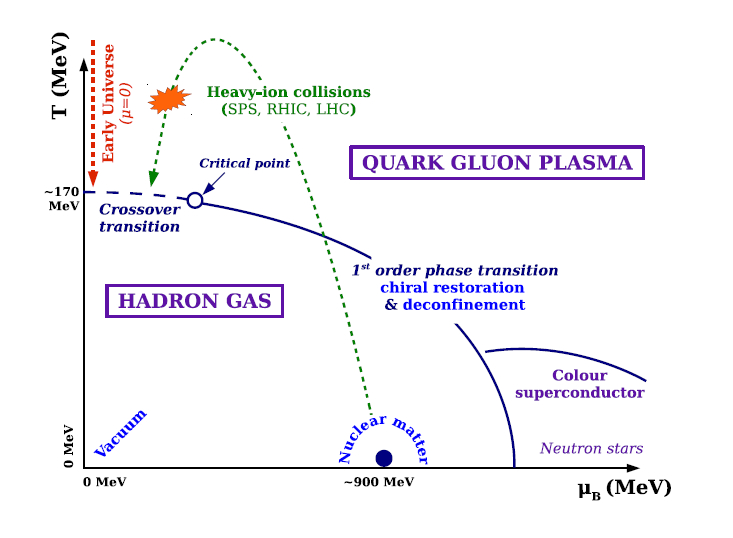
\includegraphics[width=0.8\textwidth] {FigCap1/QCDphase.jpeg}
\caption{Phase diagram of strongly interacting matter.}
\label{fig:QCDphase}
\end{figure}

Although the transformations in the early universe concerned the interactions among quarks,
this phase transition would never happened if not leaded by macroscopic
conditions, like the system temperature and density. The comprehension 
of the evolution of this state of matter 
has the promise to become accessible if we understand the thermodynamics 
laws of the QCD. It is not obvious indeed, nevertheless intriguing, 
to understand whether the QCD thermodynamics applies to the fireball 
created in the heavy-ion collisions in the laboratory, and whether the 
emitted hadrons keep a trace of the thermodynamics processes. \\

After the SPS, the Relativistic Heavy-Ion Collider (RHIC) at BNL 
has conduced experiments to create hot QCD matter through Au-Au 
collisions with the highest collision energy $\sNN = 200$ GeV per nucleon-nucleon
collision, one order of magnitude above the top of SPS energy. 
The Large Hadron Collider (LHC) at CERN is conducing experiments 
along the same line with the highest achievable center-of-mass 
energy of $\sNN = 5.02$ TeV per nucleon-nucleon collision.

\section{Micro bang vs big bang: timescales of expansion, baryonic number}
The system created in the laboratory by colliding
high-relativistic nuclei presents many similarities with 
the matter of the primordial universe, but also some differences. 
A Hubble-like expansion drives the 
evolution of the system after the collisions in the laboratory and the fireball undergoes different phases: 
\begin{itemize}
\item Pre-equilibrium phase: parton scatterings produce a large number of partons; 
they interact among each other leading the fireball to thermalize after a 
time of $\sim$ 0.6-1 fm/c;
% with the creation of high-$\pt$ probes (heavy quarks, photons) and low-$\pt$ particles;
\item QGP phase: with high-energy collisions, if the temperature inside the fireball 
exceeds the critical temperature $T_{\rm c}$, the system is in a deconfined 
phase with partonic degrees of freedom. While the phase of QGP in the early universe lasted
tens of microseconds, due to the interplay of gravity and
radiative pressure of the expanding matter, the plasma created in the laboratory 
has a lifetime of the order of 10$^{-23}$ seconds. During this time, it rapidly expands
and cools down, thus the size and local properties of
the fireball change rapidly, contrary to what happens in the 
early universe.

\item Hadronization phase: while expanding, the temperature 
of the medium drops down and, when the critical temperature $T_{\rm c}$
is reached, quarks and gluons give rise to hadrons (confinement); the hadron
gas continues the expansion and the temperature lowers further.

\item Chemical freeze-out: inelastic processes cease and the relative abundances of the various hadron species are fixed;
\item Kinetic freeze-out: even elastic collisions finish, fixing the momentum distribution of the produced particles. 
\end{itemize} 

\begin{figure}[h!]
\centering
 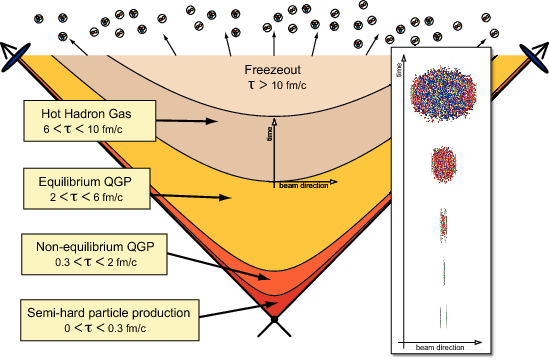
\includegraphics[width=0.8\textwidth] {FigCap1/timescales.png}
\caption{The space-time evolution of a heavy-ion collision. }
\label{fig:QCDphase}
\end{figure}


Unlike in the early universe, we expect in the laboratory a significant matter-antimatter 
asymmetry in the particle abundance, at the lower center-of-mass energies due to the
stopping of the colliding nucleons. 
At the energies of AGS and SPS, colliding nuclei tend to stop each other, forming a 
dense, baryon-rich matter and hence a system with a large $\mu_{B}$. At higher 
energies ($\sNN > 100 \Gevc$), they pass through each other leaving a nearly 
baryon-free matter in the region at central rapidity. In this case the system is closer 
to the conditions of zero baryo-chemical potential of the primordial universe. 
RICH experiments were the first to enter in the  ``baryon free'' domain. Today, ALICE, 
CMS and ATLAS, thanks to unprecedentedly high energy beams at the LHC, are 
exploring this region with even smaller baryo-chemical potential. 
Fig.~\ref{fig:YieldsVsEnergyAndronic} shows the measured yields of identified 
particles and anti-particles at mid-rapidity (rapidity being defined as 
\mbox{$y = 1/2 \; {\rm ln}((E+p_{L})/(E-p_{L}))$}, where $E$ is the particle energy 
and $p_{L}$ its momentum longitudinal to the beam direction) as a function of the 
center-of-mass energy of the collision, covering results by experiments at the 
AGS, SPS, RHIC and LHC~\cite{Andronic:2014zha}. The difference in the production 
of p and $\bar{\rm p}$ at low energies is a clear example of what discussed above. 
Because of the large stopping power in the low-$\sNN$ region, the quark content of
 the fireball is dominated by the quark content of the colliding nucleons. At LHC 
 energies, yields of particles and anti-particles are the same, 
 indicating the increasing transparency in the collision. 
The difference in the production of $\pi^+$ and $\pi^-$ at low $\sNN$ is due to the 
isospin composition of the fireball. Finally, the difference between $K^+$ and $K^-$ 
and between $\Lambda$ and $\bar{\Lambda}$ is again due to their quark content, 
$K^+ (u\bar{s})$, $K^- (\bar{u}s)$, $\Lambda (uds)$, $\bar{\Lambda} (\bar
{u}\bar{d}\bar{s})$: like in the proton case, the quark content of the colliding nucleons
drives the fireball content, whereas in regimes of large stopping power. When the collision energies become 
high enough so that the we enter the ``baryon free'' domain and particle-to-antiparticle ratios $\approx$ 1,
the baryo-chemical potential approaches $\approx 0$ values.


\begin{figure}[!t]
  \centering
  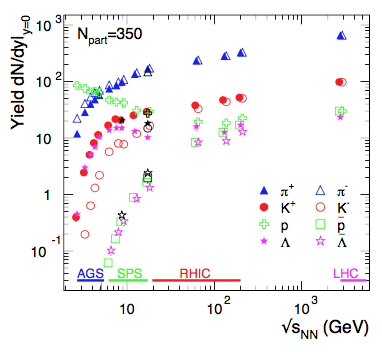
\includegraphics[width=8.5cm]{FigCap1/YieldsVsEnergyAndronic.png}
  \caption{Collision energy dependence of the multiplicities (yield, dN/dy, at mid-rapidity) of pions, kaons, protons and lambda hyperons and their antiparticles, measured in central collisions (corresponding to an average number of 350 participant nucleons in the collision) of Au or Pb nuclei~\cite{Andronic:2014zha}.}
  \label{fig:YieldsVsEnergyAndronic}
\end{figure}

% /* Expansion rates differ by 18 orders of magnitude
% Expansion in 3d, not 4d; driven by pressure gradients, not gravity
% Time scales measured in fm/c rather than billions of years
% % Distances measured in fm rather than light years
% “Heavy-Ion Standard Model” still under constructio
% Similarities: Hubble-like expansion, expansion-driven dynamical freeze-out
% chemical freeze-out (nucleo-/hadrosynthesis) before thermal freeze-out
% (CMB, hadron pT -spectra)
% initial-state quantum fluctuations imprinted on final state*/
\section{What theory tells us}
\label{sec:Lattice}
QCD is the widely accepted theory for the strong interaction. 
Phenomena at high energies, or equivalently, very short distances can be
predicted via a perturbative approach, since the coupling constant is weak. 
How the quarks are bound in the hadrons, however, is controlled by 
the large-scale behaviour of the coupling, which increases with distance. 
For such reason, Lattice Calculation is an indispensable technique. 
Lattice QCD is a non-perturbative treatment of QCD formulated 
on a discrete grid or lattice of points in space and time~\cite{Philipsen:2012nu}. 
Because of the non-perturbative nature of the theory, 
numerical simulations of Lattice QCD are the only tool 
allowing for calculations from first principles. The discretisation of the 
space-time continuum provides two main 
advantages: on one hand the problem of ultraviolet divergences typical 
of the perturbative approach is solved 
as the step of the lattice defines a shortest distance scale and hence a 
cut-off value for the momentum scale. 
On the other hand, we wish to describe a system of particles in a finite 
volume $V$, which is in thermal contact 
with a heat bath at temperature $T$. Associated with the particles, there 
may be a set of conserved charges 
$N_i$, with \textit{i}=1, 2, ... (such as the particle number, electric charge, 
baryon number etc.). In quantum field 
theory, the most direct description is in terms of the grand canonical ensemble, 
defining a density operator $\rho$ and a partition function $Z$ of the system at a temperature $T$:
\begin{equation}
\rho =e^{-\frac{1}{T}(H-\mu_iN_i)},\quad Z=Tr(e^{-\frac{1}{T}(H-\mu_iN_i)})=  \int dx \langle x|e^{-\frac{1}{T}(H-\mu_iN_i)}|x\rangle,
\end{equation}
where $\mu_i$ are the chemical potentials for the conserved charges, and 
the quantum mechanical trace is a sum over 
all energy eigenstates $|x\rangle$ of the Hamiltonian H. 
From the partition function, all other thermodynamic equilibrium quantities are 
calculable. The basic idea behind lattice 
QCD is the possibility to express the grand canonical partition function using the 
path integral representation, going in the 
domain of imaginary time. Actually, the partition function has a very similar 
formulation to the propagator of a quantum 
mechanical system between two space-time points $\langle x_b|e^{-iH(t_b-t_a)}|x_a\rangle$. 
The path integral 
formulation allows the use of Monte-Carlo methods to find the equilibrium states of the system. 
With lattice discretisation, some ``order parameters'' can be defined, which are 
sensitive to certain processes and accessible from lattice calculations. From them, 
estimates of characteristics parameters, like the critical temperature $T_c$ for the transition
to a deconfined starte, can be obtained. Among the order parameters, there are:
\begin{figure}[!t]
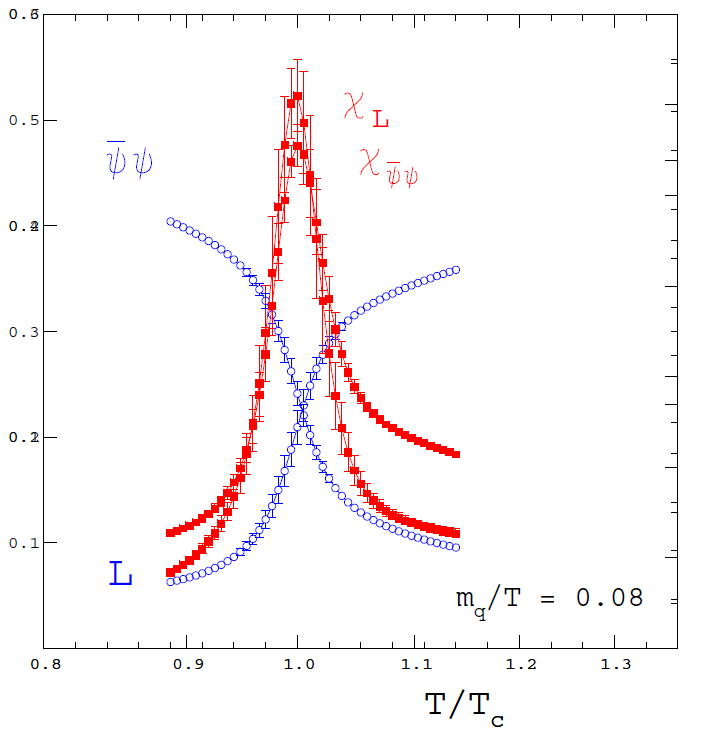
\includegraphics[width=6cm,height=6cm]{FigCap1/Lattice1.png} 
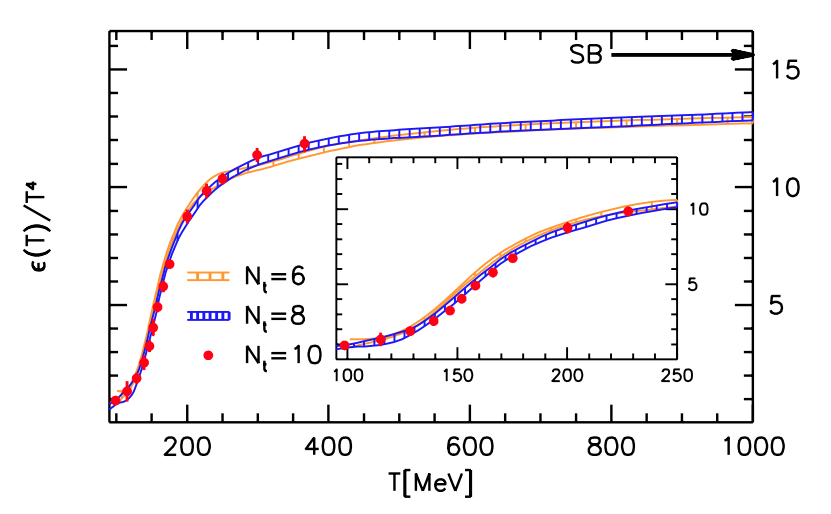
\includegraphics[width=7.5cm,height=5.8cm]{FigCap1/BW_EnDensity.png}
 \caption{(Left) Chiral condensate $\langle \bar{\psi}\psi\rangle$ and free energy function L (blue) as function of temperature. Their susceptibilities are shown in red~\cite{Karsch:2001vs}. (Right) Lattice simulation of energy density as a function of temperature. The arrows indicate the position of the Stefan-Boltzmann limit~\cite{Borsanyi:2010cj}.}
\label{fig:Lattice}
\end{figure}

\begin{itemize}
\item \textbf{Polyakov loop,} defined as:
\begin{equation}
L(T)\sim {\rm exp}\{-V(r)/T\},
\end{equation}
where $V(r)$ is the potential between a static quark-antiquark pair separated by a distance $r$. 
In pure gauge theory $V(r)\sim \sigma r$ where $\sigma$ is the string tension (two color sources 
in a confining gauge theory are bound together by a thin flux tube and this hypothesis is the
core of the effective string description of confinement~\cite{Caselle:2002vq}); hence V($\infty$) = $\infty$, 
and $L = 0$. In a deconfined medium, colour screening among the gluons leads to a melting of the 
string, which makes $V(r)$ finite at large $r$; hence $L$ does not vanish. It thus 
becomes a parameter for estimating the state of deconfinement. 
Fig.~\ref{fig:Lattice} (left) shows lattice results for $L(T)$ and the 
corresponding susceptibility $\chi_L(T)\sim \langle T^2 \rangle - \langle T \rangle ^2$. 
\item \textbf{Chiral condensate: }the effective quark mass is measured by the expectation value 
of the corresponding term in the Lagrangian, $\langle  \bar{\psi}\psi\rangle (T)$. 
The chiral symmetry is the invariance of the Lagrangian under an axial transformation of the fermion field:
\begin{equation}
\Psi \rightarrow e^{-i \gamma_{5} \frac{\vec{\tau} \cdot \vec{\theta}}{2}}\Psi
\end{equation}
where $\vec{\tau}$ are the three Pauli matrices and $\gamma_5$ 
is the chiral operator. In the limit of 
vanishing current quark masses, the Lagrangian becomes 
chirally symmetric. When confined into 
hadrons, the bare quarks ``dress'' themselves with gluons acquiring 
an effective constituent mass. 
Then, after the transition to a deconfined phase, the quarks 
would recover the "bare" mass, and the 
chiral symmetry should be approximately restored. In the calculations, 
the order parameter for the transition is the effective 
quark mass, measured as the expectation value of the corresponding 
term in the Lagrangian, that is the 
chiral condensate $\langle \overline{\psi}\psi \rangle$. In Fig.~\ref{fig:Lattice} 
(left) the behaviour of 
the order parameter as a function of temperature is shown. 
Recent results provide a measure of the critical temperature 
$T_c$ from the results for the chiral condensate, 
and it is estimated as $T_c = (154 \pm 9) $ MeV~\cite{Petreczky:2012rq}.
\item \textbf{Energy density $\epsilon$ and pressure P} at deconfinement: 
in Fig.~\ref{fig:Lattice} (right) it 
is seen that $\epsilon/T^4$ changes quickly at the critical temperature 
$T_c$, increasing from a low 
value typical of an hadron gas to a higher value closer to what expected 
for an ideal gas in the Stefan-Boltzmann limit of 
massless quarks and gluons. N$_{\rm t}$ is the number of points in the temporal
direction of a hypercubic lattice~\cite{Borsanyi:2010cj}. The 
remarkable deviation of $\epsilon/T^4$ from the
Stefan-Boltzmann limit is a clear signal of surviving
correlations in the deconfined phase.
The rapid increase in energy density is expected to occur as consequence of the increased number of degrees of 
freedom in the phase transition. %Recent calculations of Lattice QCD predicts as critical temperature $ \sim 160$ MeV~\cite{Karsch:2001vs}.

\end{itemize}


\begin{figure}[!b]
  \centering
  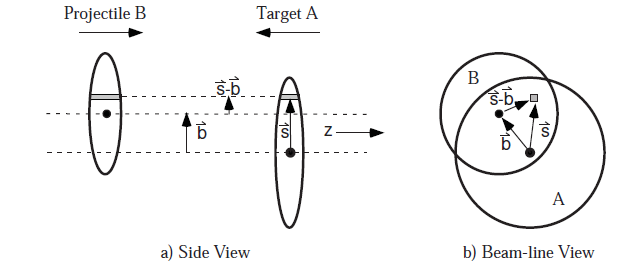
\includegraphics[width=12cm]{FigCap1/glauber.png}
  \caption{Schematic view of a nucleus-nucleus collision described in terms of the impact parameter b in the longitudinal (left) and transverse (right) plane.}
  \label{fig:image10}
\end{figure}

\section{Collision Geometry and the Glauber Model}
In a collision of two nuclei, the impact parameter \textit{b}, i.e. the distance 
between the centers of the nuclei in the transverse plane of the collision, can 
span values from 0 to about $R_1+R_2$, where  $R_1$ and  $R_2$ are the radii of 
the two nuclei if approximated with hard spheres. 
Small values of $b$ ($\lesssim$ 3.5 fm) imply central collisions. 
The impact parameter can not be measured directly, still it is 
possible to relate it to observables as the multiplicity of particles produced in the 
collision, the transverse 
energy or the number of spectator nucleons. 
The Glauber model is used to calculate the geometrical quantities that 
characterize the collision (such as the number of nucleons participating in the collisions,
the number of spectator nucleons), and that can be correlated with some
observables (such as multiplicity, transverse energy) to estimate the centrality of the
collision~\cite{Miller:2007ri}.
The model provides a phenomenological description assuming that the nucleus-nucleus 
collision can be treated as a superposition of independent nucleon-nucleon collisions.
Under the assumptions (optical limit) that, (i) at sufficiently high energies, the nucleons 
inside the nuclei are essentially undeflected after the collision, (ii) the
 nucleons are independent in the nucleus, (iii) protons and neutrons 
 are indistinguishable and (iv) the radius of the nucleus is large compared 
 to the extent of the nucleon-nucleon force, we can define the thickness 
 functions of nuclei A, B for a certain value of impact parameter $b$ (see Fig.~\ref{fig:image10}):
\begin{equation}
T_i(\vec s) = \int\,dz \rho_i(\vec s,z).
\end{equation}
The thickness function is related to the nuclear density function $\rho$. The nuclear 
density is usually parameterized by a Woods-Saxon or 3-parameter Fermi distribution:
\begin{equation}
\rho (r) = \rho_0 \frac{1+w(r/R)^2}{1+{\rm exp}(\frac{r-R}{a})},
\end{equation}
where $\rho_0$ is the nuclear density in the center of the nucleus, 
$R = (6.62 \pm 0.06)$ fm is the radius parameter of the ${}^{208}$Pb, 
$a = (0.546 \pm 0.010)$ is the skin thickness of the Pb nucleus and $w$ 
characterizes deviations from a spherical shape ($w=0$ for Pb). 
The nuclear overlap function is then defined as:
\begin{equation}
T_{AB} = \int \,d^2s T_A(\vec s)T_B(\vec s - \vec b)
\end{equation}
and it gives the probability for two incoming nucleons inside two nuclei colliding 
with impact parameter \textit{b} to be in the same elementary area $d^2s$ in the transverse plane.
By considering the mean of a binomial distribution, the average number of 
binary nucleon-nucleon collisions $\langle N_{coll}\rangle$ as a function 
of the impact parameter \textit{b} can then be written as:
\begin{equation}
\langle N_{coll}\rangle = AB \times T_{AB}(b)\; \sigma^{inel}_{NN},
\end{equation}
where $A$ and $B$ are the mass numbers of the colliding nuclei and $\sigma^{inel}_{NN}$
is the inelastic interaction cross-section of the two nucleons.
The average number of participant nucleons in the collisions (nucleons of target 
and projectile that interact) can be obtained as a function of the impact parameter $b$ as:
\begin{equation}
\begin{aligned}
N_{part} (b) &= \int A \; T_A(\vec{s}) [1- (1- \sigma_{inel} T_B(\vec{b}-\vec{s}))^B]d^2s \\
& + \int B \; T_B(\vec{b}-\vec{s}) [1- (1- \sigma_{inel} T_A(\vec{s}))^A]d^2s.
\end{aligned}
\end{equation}
The inelastic cross-section for a collision between two nuclei (A and B), 
in a certain centrality range ($0 < b < b_c$) 
can be expressed using the Glauber model geometry, as:
\begin{equation}
\label{eq:sigmaABGlauber}
\sigma_{AB}(b_c) = \int_0^{b_c} 2\pi b\,db [1 - (1 - \sigma^{inel}_{NN}T_{AB}(b))^{AB}]. %\simeq \int_0^{b_c} 2\pi b\,db \cdot AB\cdot T_{AB}(b)  \sigma^{inel}_{NN}.
\end{equation}
\begin{figure}[!t]
\centering
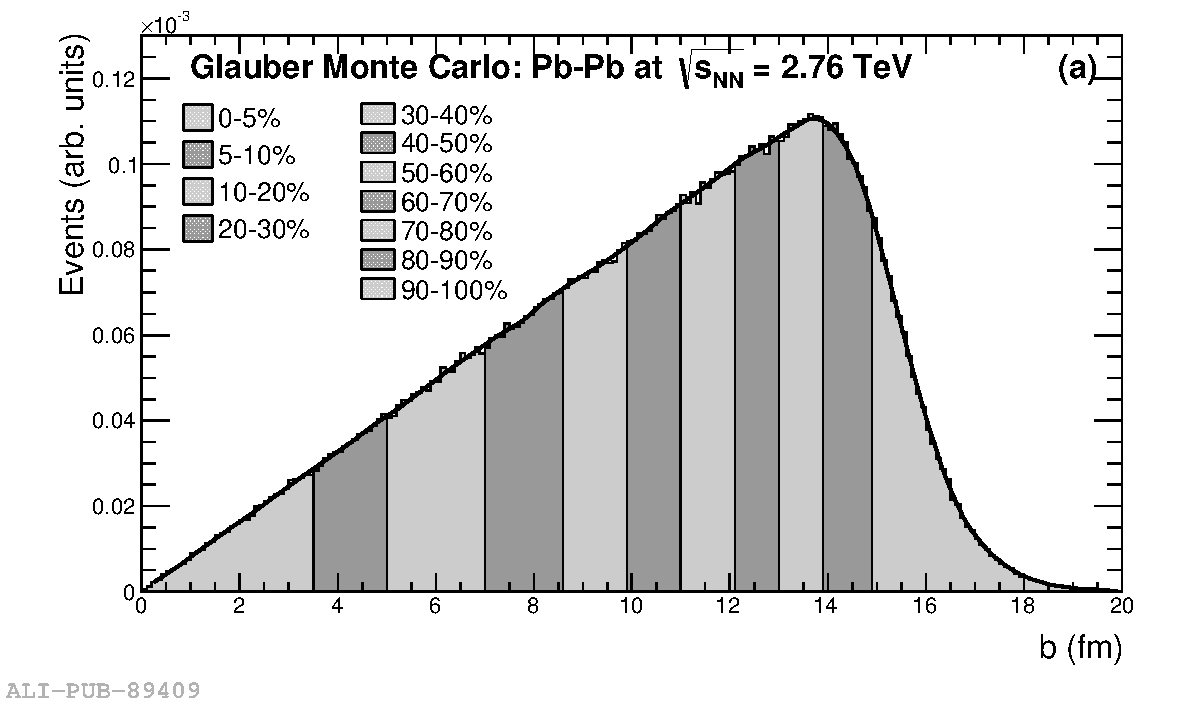
\includegraphics[width=7cm]{FigCap1/Glauberimpactpar.pdf}
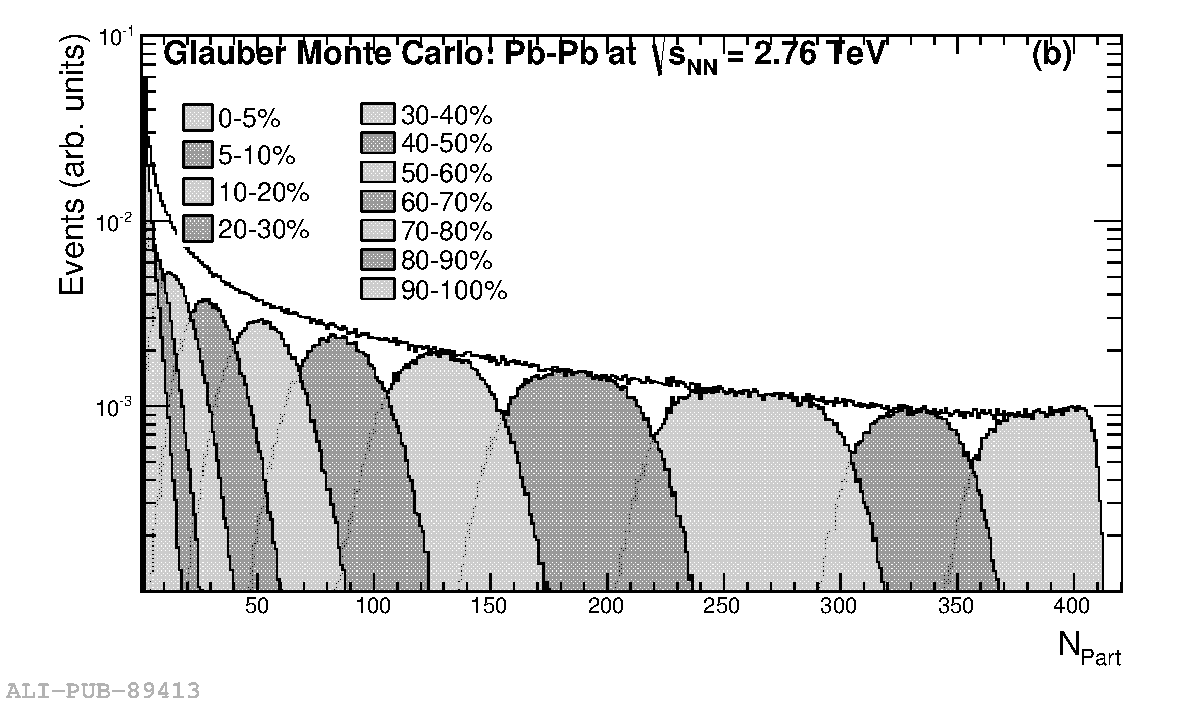
\includegraphics[width=7cm]{FigCap1/GlauberNpart.pdf}
\caption{Left: impact parameter distribution obtained from Glauber MC simulations for Pb-Pb collisions at $\sNN = 2.76$ TeV. Right: the corresponding $N_{\rm part}$ distributions for different intervals of centrality percentiles.}
\label{fig:glaubMC}
\end{figure}
The centrality is usually expressed in terms of percentiles of the total nuclear 
interaction cross section $\sigma_{AB}$ in Eq.~\ref{eq:sigmaABGlauber}.
The percentile of the cross-section for collisions in a given impact parameter
interval $b_{min}<$ b $<b_{max}$ (see Fig.~\ref{fig:glaubMC}) is given by:
\begin{equation}
c=\frac{1}{\sigma_{AB}}\int_{b_{min}}^{b_{max}} \frac{d\sigma_{AB}}{db'}db'.
\end{equation}
A simple approach to utilize the Glauber Model formulation for the
 calculation of geometry related quantities like $N_{part}$ and $N_{coll}$
is a Monte Carlo implementation. 
Furthermore, it is possible to simulate experimental quantities 
like the charged particle multiplicity and to apply similar centrality cuts as in the analysis of real data. 
In the simulation the nucleon distribution in the two colliding nuclei is randomly generated
according to their nuclear density distributions.
A random impact parameter $b$ is also associated to the collision according to the distribution
d$\sigma$/d$b \propto 2\pi b$. The nucleons travel on straight-line
trajectories and the inelastic nucleon-nucleon cross-section is assumed to be independent
of the number of collisions a nucleon underwent before. A nucleon-nucleon collision takes place if
their distance $d$ in the plane orthogonal to the beam axis satisfies:
\begin{equation}
d \leq \sqrt{\sigma^{inel}_{NN}/\pi}.
\end{equation}
Optical Glauber and MC Glauber show good agreement when calculating 
simple geometric quantities like $N_{part}$ and $N_{coll}$ as
a function of impact parameter. Some discrepancies appear at the highest impact parameters.
This is mainly due to the fact that in the Optical Approximation the incoming nucleon sees the incoming nucleus as a smooth density object and does not account for event-by-event density fluctuations.



In Chapter 3, more details will be given about the calculation 
of N\textsubscript{part} and N\textsubscript{coll} and the centrality 
determination in the ALICE experiment.


\section{Heavy-ion physics at the LHC}
Let's now turn into the experiments. The SPS program, with its several experiments, 
was mainly aimed at understanding whether a new state of matter, with the 
characteristics of a Quark-Gluon Plasma, could actually be created in the laboratory.
For a more quantitative study of the properties of this
system, we had to wait for the following research era, with the RHIC and LHC colliders.
However, the first results from the SPS revealed that Pb-Pb collisions 
were not simply a trivial superposition of elementary proton-proton (pp) collisions.
First of all, it was possible to measure quantitatively
the energy density and temperature of the fireball formed after collisions of two Pb nuclei.
A formula derived by Bjorken~\cite{Bjorken} 
revealed the energy density of the system to be around
3 GeV/fm$^{3}$, slightly above the phase transition
that the Lattice QCD predicts to be at about 0.5-0.6 GeV/fm$^3$~\cite{Hands}. At that energy density,
Lattice QCD gives a plasma temperature of about 210 MeV. The main experimental observations at the SPS 
were an abundant production of hadrons
containing strange quarks~\cite{Sandor:2004bg} (``strangeness enhancement"), 
the reduced production of the J/$\psi$ mesons~\cite{Abreu:2000ni} 
(``anomalous J/$\psi$ suppression") and the yields of 
low-mass lepton pairs~\cite{Damjanovic:2005ni} (``$\rho$ melting"). They constituted 
the signals that a new state of matter had been found.
Moreover, the NA49 experiment gave the first indications that the fireball medium 
could be described by QCD hydrodynamics, with the measurement
of the elliptic flow of pion and proton in semi-peripheral Pb-Pb collisions 
at top SPS energy~\cite{Alt:2003ab}. This observable, described in more detail 
in Sec.~\ref{sec:AnisotropicFlow}, is related with the
initial spatial anisotropy of the overlapping area of the two colliding nuclei, that is 
then converted into a final momenta anisotropy. Such a process is only possible 
if the fireball is guided by collective motion effects in a liquid-like medium with  
small viscosity. The initial results from RICH confirmed the picture 
of an extremely strongly interacting and almost perfect liquid QGP, enough opaque 
to quench any fast parton that travels througth.\\
This effect and the experimental observations mentioned before will be deeper 
explored during the LHC phase. We will go now through a revision of some of the most 
important results and open points regarding heavy-ion physics at the higher LHC energies. 

\begin{figure}[!t]
  \centering
  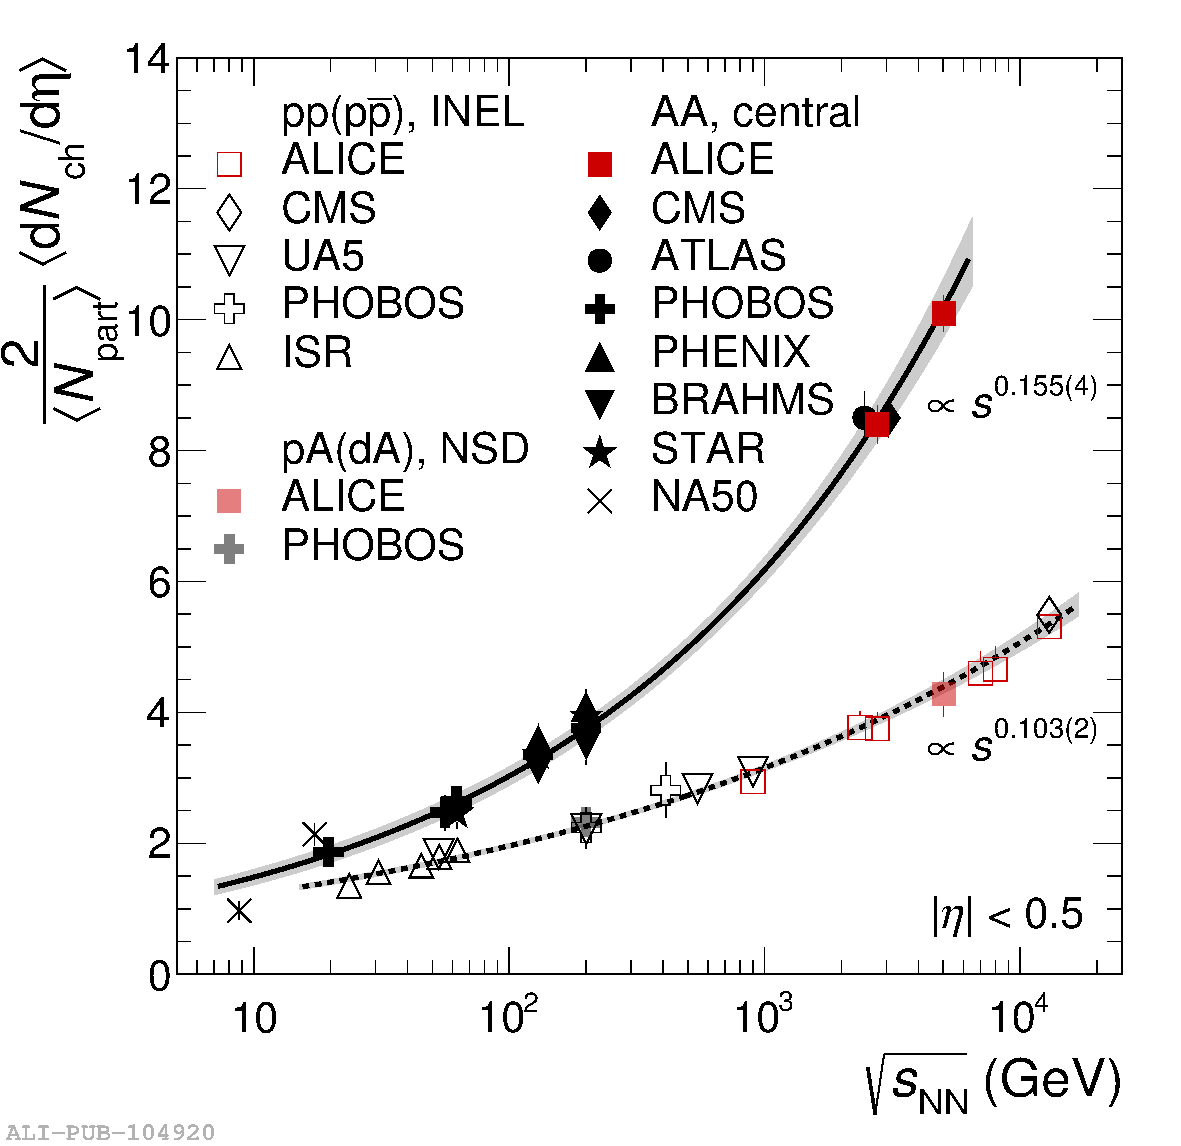
\includegraphics[width=7cm]{FigCap1/dNchdEtaVsEnergy.pdf}
  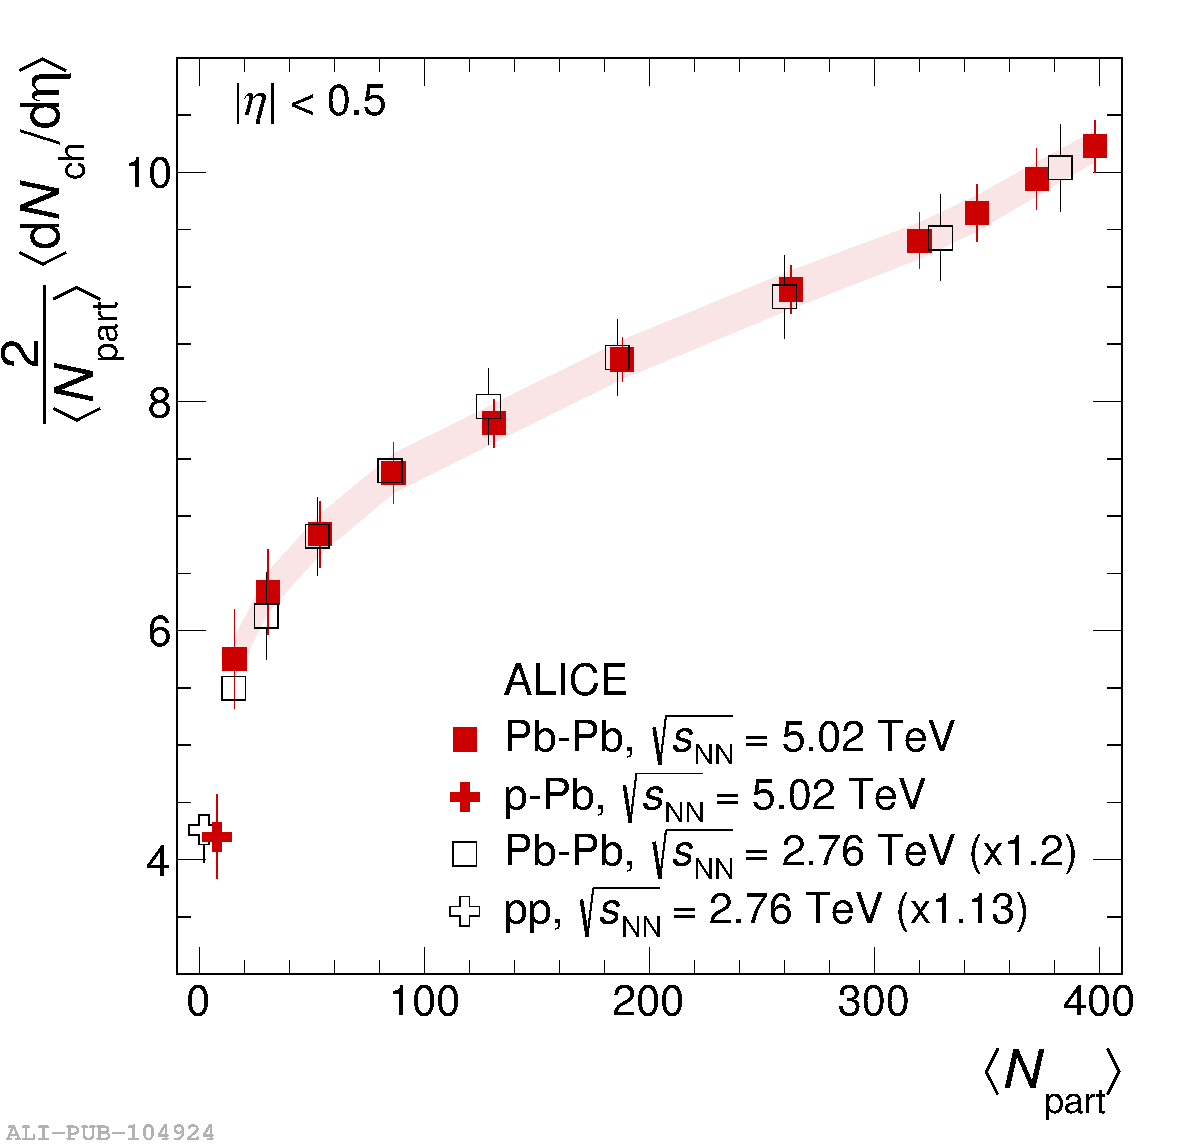
\includegraphics[width=7cm]{FigCap1/dNchdEtaVsNpart.pdf}
  \caption{(Left) Charged particle pseudo-rapidity density per participant pair for pp and central AA collisions as a function of center-of-mass energy per nucleon pair, measured in different colliding systems~\cite{Adam:2015ptt}. The fit to the power law is shown as solid (A-A) and dashed (pp) lines, together with the uncertainties on the dependence (shaded bands). (Right) Centrality dependence of (d$\Nch$/d$\eta$)/($\langle N_{\rm part} \rangle/2$) for p-Pb and Pb-Pb collisions at $\sNN=5.02$ TeV~\cite{ALICE:2012xs,Adam:2015gka}, Pb-Pb collisions at $\sNN=2.76$ TeV~\cite{Aamodt:2010cz} and pp collisions at $\sqrt{s}=7$ TeV measured with ALICE.}
  \label{fig:dNchdEta}
\end{figure}

\subsection{Particle multiplicity and energy density}
The number of particles produced in the collision (multiplicity) is related to the 
density of the created medium. Particle multiplicity depends in fact both on the 
centrality and energy of the collision. This observable is usually presented as 
a pseudo-rapidity ($\eta = - {\rm ln}(\tan(\theta/2))$ density of charged particles at 
mid-rapidity (d$\Nch$/d$\eta |_{\eta=0}$). This is useful to compare experimental 
results with different acceptances. Furthermore, particle density is usually 
divided by the average number of nucleon pairs participating to the collision 
($\langle N_{\rm part}\rangle$/2), to compare results from different 
colliding systems. The measurements by ALICE in the 5\% 
most central Pb-Pb collisions at $\sNN = 5.02$ TeV found a density of charged 
particles at mid-rapidity $\langle $d$\Nch$/d$\eta \rangle = 1943 \pm 54$ 
and, normalised per participant pair, (d$\Nch$/d$\eta$)/($\langle N_{\rm part} \rangle/2$) $ 
= 10.1 \pm 0.3$~\cite{Adam:2015ptt}.  
The left panel of Fig.~\ref{fig:dNchdEta} presents (d$\Nch$/d$\eta$)/($\langle N_{\rm part} \rangle/2$) 
as a function of the center-of-mass energy per nucleon pair. The energy dependence 
of the charged multiplicity for central heavy-ion collisions can be fitted with a power 
law of the form $as^b$, where $b = 0.155 \pm$ 0.004~\cite{Adam:2015ptt}. 
The rise is much stronger than for pp collisions where $b = 0.103 \pm 0.002$, 
obtained from a fit to the same function. It can also be noticed that the values 
of (d$\Nch$/d$\eta$)/($\langle N_{\rm part} \rangle/2$) from p-Pb collisions are included in the figure 
and lays on the pp curve, indicating that the strong rise in A-A collisions is not 
only related to the multiple interactions undergone by the participating nucleons, 
present in p-A collisions as well. The right panel of Fig.~\ref{fig:dNchdEta} 
shows the values of (d$\Nch$/d$\eta$)/($\langle N_{\rm part} \rangle/2$) 
as a function of the average number of participant nucleons 
measured by ALICE in p-Pb~\cite{ALICE:2012xs} and Pb-Pb~\cite{Adam:2015ptt} 
collisions at $\sNN = 5.02$ TeV. The Pb-Pb measurements at 
$\sNN = 2.76 $ TeV~\cite{Aamodt:2010cz} are also shown, scaled by a 
factor of 1.2 (calculated from the observed $s^{0.155}$ dependence), as 
well as the pp measurements at $\sqrt{s}= 7$ TeV~\cite{Adam:2015gka} 
scaled by a factor of 1.13. The charged particle density per participant pair 
shows a strong dependence on $\langle N_{\rm part}\rangle$, decreasing 
by a factor of about 1.8 from most central collisions to peripheral ones. The 
measurement of particle production per participant pair can be used to 
constrain models describing particle production in heavy-ion collisions 
with different mechanisms. Among the others, theoretical calculations that
 are based on gluon saturation 
 (rcBK-MC~\cite{Albacete:2011fw}, Kharzeev, Levin and Nardi~\cite{Kharzeev:2004if} 
 and Armesto, Salgado and Wiedemann~\cite{Armesto:2004ud}) can 
 give a good description of data. They are based on the idea of some 
 transverse momentum scale at which the gluon and quark phase space 
 density saturates, thus limiting the number of produced partons and, 
 hence, of particles produced in heavy-ion collisions with respect to pp collisions.  
 This results also in a centrality dependence of the multiplicity of 
 heavy-ion collisions in the models, as observed in the experimental
data. \\
The simplified Bjorken model~\cite{Bjorken:1982qr} can be used to 
estimate the initial spatial energy density from the measured 
$\langle$d$\Nch$/d$\eta$$\rangle$:
\begin{equation}
\label{Bjorken}
\epsilon_{Bj} = \frac{\langle m_T\rangle}{\tau_f A}\frac{dN_{\rm ch}}{dy}
\end{equation}
where $\tau_f$ is the formation time of the secondary particles, A is the overlap 
area of the two colliding nuclei, $\langle m_T \rangle$ is the average transverse 
mass of the created particles defined as $m_{T} = \sqrt{m^{2}+\pt^2}$ and $y$ 
is the rapidity. Starting from the measured values of d$\Nch$/d$\eta$, it is 
possible to estimate the energy density of the medium created in the collision.
At top RICH energy (200 GeV), for the most central collisions, one obtains 
$\sim 5$ GeV/fm$^3$ at the conservative estimate for the formation time 
$\tau_f$ = 1 fm/c~\cite{Bjorken:1982qr}, well above the critical value predicted 
by lattice QCD for the phase transition to QGP. For central Pb-Pb collisions at the LHC 
at $\sNN$ = 2.76 TeV the value of $\epsilon_{Bj}$ is much higher and is 
around $\sim 14$ GeV/fm$^3$~\cite{Chatrchyan:2012mb}.

\subsection{Hadron multiplicities and chemical freeze-out}
If a chemical and thermal equilibrium governs the medium when it
 undergoes chemical freeze-out, the thermal nature of the medium 
 can be expected to be imprinted in the final hadron abundances. 
 If these conditions occur, the behavior of the system at the 
 equilibrium can be described via a statistical approach, using a description 
 of the final particle yields in terms of thermodynamical quantities. 
 Following the approach described in~\cite{BraunMunzinger:2003zd}, 
 we can introduce the partition function Z($T,V,\mu_{Q}$), that 
 allows for a quantitative description of the statistical properties 
 of the equilibrated system, as a function of temperature $T$, 
 volume $V$ and chemical potentials $\mu_{Q}$. 
\begin{figure}[!ht]
  \centering
  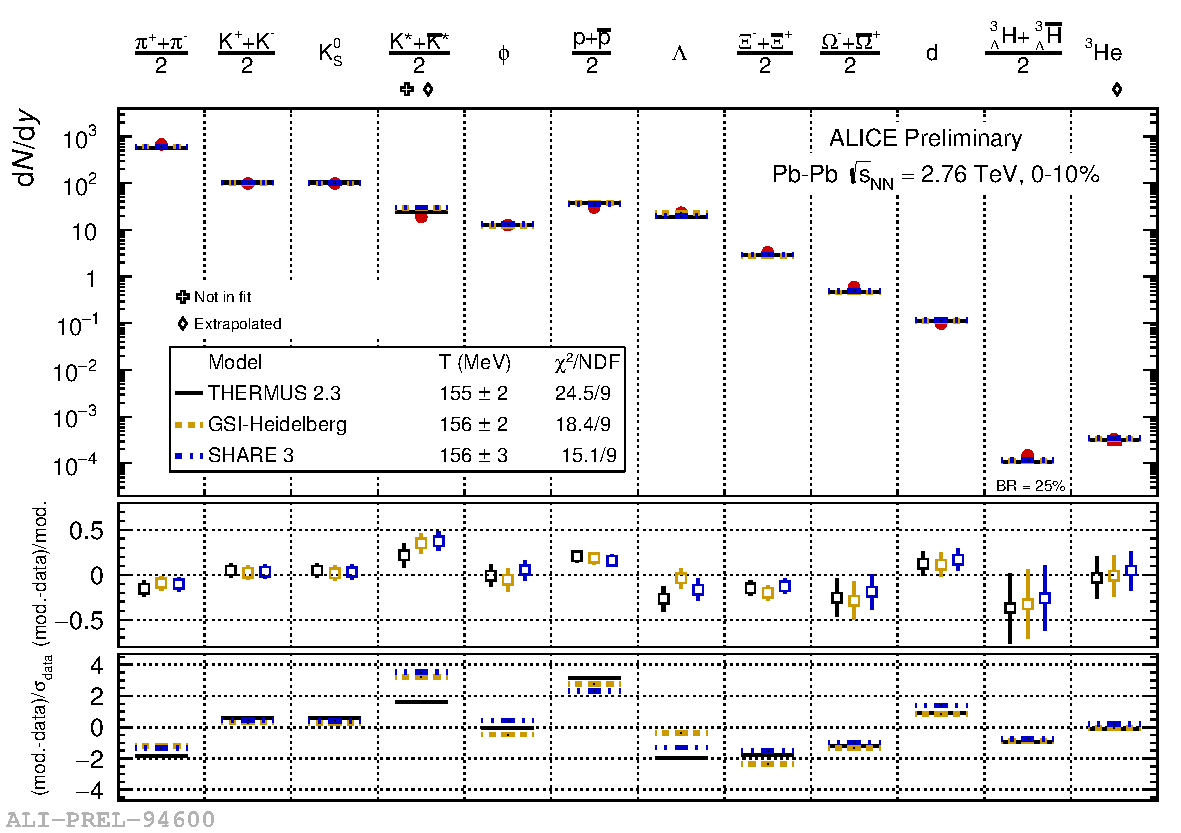
\includegraphics[width=12cm]{FigCap1/GCThermalFit_PbPb010.pdf}
  \caption{Grand Canonical thermal fit to ALICE 0-10\% Pb-Pb data at $\sqrt{s_{\rm NN}} = 2.76$ TeV~\cite{Floris:2014pta}. Excluded volume correction implemented in THERMUS and GSI with r = 0.3 fm, $\mu_{B}$ fixed to 0, $\gamma_{s}$ fixed to 1, $\gamma_{c}$ fixed to 20. }
  \label{fig:GCThermalFit_PbPb010}
\end{figure}

In the Grand Canonical (GC) ensemble, which describes a system in which 
energy and charges are on-average conserved within the full volume, the partition function is:
\begin{equation}
  \label{eq:PartitionFunction}
Z^{\rm GC} (T, V, \mu_{Q}) = {\rm Tr}[e^{-\beta(H - \sum_{i}{\mu_{Q_{i}}Q_{i}})}],
\end{equation}
where $H$ is the Hamiltonian of the system, $Q_{i}$ are the conserved charges, 
$\mu_{Q_{i}}$ are the chemical potentials needed to guarantee charges 
conservation on average in the whole system and $\beta = 1/T$ is 
the inverse temperature. At the leading order, the Hamiltonian of a non-interacting 
hadron-resonance gas contains all the degrees of freedom of a 
confined, strongly interacting medium. Further corrections can be added by 
introducing hadron repulsions, generally Van der Waals-like interactions. 
In the hadron-resonance gas a hadron mass 
spectrum containing mesons with masses below $\sim 1.5 \; \Gevcc$ and 
baryons with masses below $\sim 2\; \Gevcc$ is considered. In this mass interval, the 
hadronic spectrum is well known as well as the decay channels of resonances 
and particles. With these assumptions, the maximum temperature for which
 the model can be considered trustable is $\sim 200$ MeV. The GC partition 
 function of a non-interacting system, like that of our hypothesis, is given by 
 the product of the independent partition functions of all the hadronic species. 
 In the logarithmic form we write:
\begin{equation}
  \label{eq:LnPartFunction}
{\rm ln} Z(T, V \vec{\mu}) = \sum_{i} {\rm ln} Z_{i} (T, V, \vec{\mu}),
\end{equation}
where $\vec{\mu} = (\mu_B, \mu_S, \mu_Q)$ are the chemical potentials 
related to the baryon number, strangeness and 
electric charge, and the sum is over all hadron species $i$.
The density of particles of species $i$ can be obtained from Eq.~\ref{eq:LnPartFunction} as:
\begin{equation}
\label{eq:ParticleDensity}
n_{i} (T, \vec{\mu}) = \frac{\langle N_{i} \rangle}{V} = \frac{1}{V}\frac{\partial (T {\rm ln}Z_i^{GC})}{\partial \mu_i} = \frac{T g_{i}}{2\pi^{2}} \sum_{k=1}^{\infty} \frac{(\pm 1)^{k+1}}{k} \lambda_{i}^{k} m_{i}^{2}K_{2}(\frac{km_{i}}{T}),
\end{equation}
where (+) is for fermions and (-) for bosons, $g_{i}$ is the spin-isospin 
degeneracy factor, $\lambda_{i} = e^{Q_{i}\mu_{i}}$ is the fugacity 
term and finally $K_{2}$ is the modified Bessel function.
Further corrections to the particle density are necessary at high 
temperature ($\gtrsim 100 $ MeV) or density, where the contribution 
to the particle yield $N_{i}$ from resonance decays becomes 
dominant with respect to the thermal production of the species. 
Other deviations from the GC description can be taken into 
account by introducing parameters for strange, charm or 
light quarks ($\gamma_{S}, \gamma_{C}$ and $\gamma_{q}$) 
production. For example, in case there is no thermalisation for 
the strangeness component in the medium, a factor 
$\gamma_{s}<1$ is needed, usually whenever the size of system 
is small (i.e. pp collisions) or at low collision energies. 
The usage of $\gamma_{q}$ is only applied in the so called 
non-equilibrium model SHARE~\cite{Petran:2013lja}. This model 
describes an expanding, super-cooled quark-gluon plasma which 
undergoes a sudden hadronization without further re-interactions.
Among the five parameters of Eq.~\ref{eq:ParticleDensity} 
($T, V, \mu_B, \mu_S, \mu_Q$), up to three can be fixed with
 the knowledge of the conditions of the initial state. 
 The other two parameters can be obtained by fitting the measured
  particle yields. In Fig.~\ref{fig:GCThermalFit_PbPb010}, a 
  Grand-Canonical thermal fit with three different models using 
  T and V as free parameters is performed on the $y$-differential 
  identified particle yields measured by ALICE in the 10\% most 
  central Pb-Pb collisions at $\sqrt{s_{\rm NN}} = 2.76$ TeV~\cite{Floris:2014pta}. 
  The fit quality is not fully satisfactory ($\chi^{2}/ndf \sim 2$), 
  while it used to be of order 1 for RHIC energies~\cite{Andronic:2008gu}. 
  The temperature, as parameter of the fit, results to be of the order of 155 MeV. 
The measured p and $\Xi$ yields have a bad agreement with the fit 
(2.5 $\sigma$ and 2 $\sigma$ respectively). The measurements of resonances 
in central Pb-Pb collisions suggest elastic re-scattering in the late 
hadronic phases, that becomes quite important for pion production. 
If protons are excluded from the fits, the fit quality improves and the 
temperature goes up to $\sim$160 MeV (closer to RHIC results). 
Non-equilibrium models like SHARE describe most hadrons very 
nicely but overestimate the nuclei by almost an order of magnitude, 
while the equilibrium model predicts them very nicely. An other possible
interpretation is that inelastic processes during the hadronic phase may
not be completely negligible, rather affecting baryon production. In 
particular, baryon annihilation in the hadronic phase should lead
to a reduction of the proton yields~\cite{Becattini:2014hla,Becattini:2012xb}. Other models 
suggest that a single freeze-out temperature is not enough to describe
 the data~\cite{Bellwied:2013cta}, but temperature for lighter and heavier
  quarks could be different. So far, the production mechanism is not yet 
  clearly understood as well as how the temperature from the thermal 
  fit relates to the QCD phase transition temperature.
  
\subsection{Strangeness enhancement}
\label{subsec:StrangEnhancSPS}
The original idea of enhanced production of hadrons containing strange quarks 
as a signature of the quark deconfinement was proposed in 1980 by Rafelski 
and Hagedorn \cite{PhysRevLett.48.1066},\cite{Muller:2011tu}. As there are no 
strange quarks in the colliding nuclei, it follows that all strangeness must be 
created in the collision or in the QGP phase. Strange quarks are hard to 
produce at temperatures below $T_c$ since their effective mass is larger 
than $T_c$ when chiral symmetry is broken, but easy to produce at temperatures 
above $T_c$ since the current mass of the strange quark is $m_s \sim 100$ MeV/$c^2$, 
due to chiral symmetry restoration (see Sec.~\ref{sec:Lattice}). 
\begin{figure}[!ht]
  \centering
  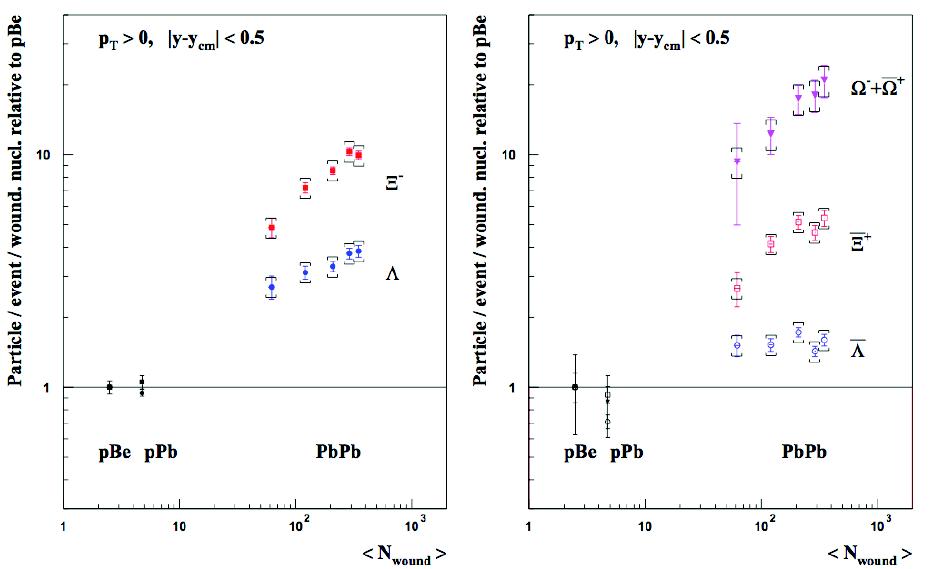
\includegraphics[width=12cm]{FigCap1/strangEnhancSPS.png}
  \caption{ Hyperon enhancement as a function of the number of the wounded nucleons measured by the NA57 experiment in Pb-Pb collisions at $\sNN = 17.2$ GeV~\cite{Sandor:2004bg}.}
  \label{fig:sEnhancSPS}
\end{figure}
For $T > T_c$, also \textit{u} and \textit{d} quark masses 
decreases to $m_q \sim 0$ MeV/$c^2$, but the 
strange quark production becomes important. In a simple hadron gas, 
even if it is possible to produce strange particles from some inelastic 
scattering such as $\pi^0+p \rightarrow K^++\Lambda$, it is less probable 
to produce multi-strange baryons, like $\Xi ^-$ and $\Omega$, as 
they are the result of more than one consecutive reactions. In presence 
of QGP, instead, it is expected an enhancement in the production of 
multi-strange baryons relative to pp reactions of about one order of magnitude.
The abundant strangeness production in QGP is due to the large gluon 
density of the system, which favours gluon-fusion processes
$gg \rightarrow s\bar{s}$. 
The Grand Canonical (GC) formulation is used whenever the conservation law of
a quantum number, for example strangeness, can be on average implemented by using
the corresponding chemical potential. This approach can be used in systems 
with a large number of produced particles. For smaller systems like pp or pA
collisions, this is no longer valid and the Canonical (C) formulation must be used
in turn. The canonical conservation of quantum numbers strictly reduces the phase
space available for particle production~\cite{Beutler:2009cc}, and this is usually referred to as canonical suppression~\cite{Tounsi:2001ck}.
This is the essence of the strangeness enhancement from pp to AA collisions.\\
In experiments the magnitude of strangeness production is usually estimated by measuring 
the enhancement factor, defined as the ratio of the yields of a given particle 
specie per participant nucleon in nucleus-nucleus collisions over the same 
ratio measured in smaller system (pp or pA). The first evidence of 
strangeness enhancement was measured by the NA57 and WA97 
collaborations~\cite{Sandor:2004bg} in fixed-target Pb-Pb collisions at 
$\sqrt{s_{NN}}$= 17.2 GeV. The enhancement factor measured by NA57 
is shown in Fig.~\ref{fig:sEnhancSPS} for $\Lambda$, $\Xi^-$ (left) and 
their anti-particles (right) in p-Pb, p-Be and Pb-Pb collisions as a function 
of the number of participating nucleons. It is observed a hierarchy for these 
enhancement factors in Pb-Pb collisions, depending on the strangeness
 content of the particles and also on the collision centrality. In p-Be and in 
 p-p there is no evidence of strangeness enhancement. 

\subsection{Collective flow and kinetic freeze-out}
The Flow is a collective phenomenon, which is observed as a collective 
motion pattern superimposed to the chaotic thermal motion of the 
particles inside the fireball. Its origin is related to the large pressure gradients 
generated when compressing and heating nuclear matter. It is possible 
to distinguish between different types of flow. In the following, 
the radial and the anisotropic flow in the transverse plane are discussed. 

\subsubsection{Radial flow}
\label{sec:RadialFlow}
For what concerns the particle production in pp collisions, 
following the approach in~\cite{Schnedermann:1993ws} we 
can treat the invariant yield of low $\pt$ particles of a given species as radiated by a
 thermal source with temperature $T$:
\begin{equation}
\label{eq:ThermalSource}
E\frac{d^{3}n}{d^3p} = \frac{dn}{dy \; m_{T} dm_T\;d\varphi} = \frac{gV}{(2\pi)^3}E\;e^{-(E-\mu)/T},
\end{equation}
  where $g$ is the spin-isospin degeneracy factor for the considered particle 
  species, $\mu$ is the grand canonical potential $\mu = n\mu_{B}+ s\mu_S$, 
  originating from the quantum numbers $n$ and $s$ for baryon and 
  strangeness content, $y$ is the rapidity, $m_{T}$ the transverse 
  mass and $\hbar = c = k_B = 1$. By integrating Eq.~\ref{eq:ThermalSource}
   over rapidity using the modified Bessel function $K_1$, we obtain
    the transverse mass distribution $dn/(m_Tdm_T)$, which behaves 
    asymptotically like a decreasing exponential for transverse masses 
    larger than the source temperature: 
\begin{equation}
\label{eq:SpectraBZ}
\frac{dN}{m_T dm_T} = \frac{V}{2\pi^2} m_T K_1 (\frac{m_T}{T}) \xrightarrow{m_T \gg T} V^\prime \sqrt{m_T} e^{-m_T/T}.
\end{equation}
It has been experimentally verified in pp collisions the universality, at low $\pt$,
of the temperature $T$ of the exponential slope of Eq.~\ref{eq:SpectraBZ}. 
In the low-$\pt$ region ($\lesssim 1 \, \Gevc$), indeed, particles originate from soft processes
and their production is governed by a Boltzmann exponential distribution. 
This law does not anymore describe production at higher $\pt$, where hard processes
govern particle emission and the production spectra result better reproduced by power law functions.
 The physical interpretation of $T_{slope}$ is the temperature of the particle
 emitting source. The universality of $T_{slope}$ for different 
 particle species is commonly referred to as $m_{T}$-scaling. When 
 moving to nucleus-nucleus collisions, a breaking of the $m_T$-scaling 
 occurs at low $\pt$ and the slopes of the spectra are observed to 
 decrease with increasing particle mass~\cite{Appelshauser:1998yb,Arnaldi:2007ru}.
  The effect is present at all centralities, but it is stronger for central
   collisions. The slope of the exponential law, at low $\pt$, can be expressed as:
\begin{equation}
\label{eq:Tslope}
T_{slope} = T_{fo} + \frac{1}{2}m \beta_{\rm T}^{2},
\end{equation}
where the second term accounts for the dependence on the mass 
and the velocity is related to the radial flow, i.e. the collective velocity
 arising from the expansion of the fireball. The first term still accounts
  for the Brownian motion of the particles, present in Eq.~\ref{eq:SpectraBZ}.
   This is the idea developed within the Boltzmann-Gibbs blast-wave 
   model~\cite{Schnedermann:1993ws}, where the radial expansion 
   velocity distribution $\beta_{\rm T}(r)$ in the region \mbox{$0 \leq r \leq R$} 
   is parametrized by relating it to the surface velocity $\beta_s$ via:
\begin{equation}
\label{eq:Br}
\beta_{\rm T} (r) = \beta_s \Big(\frac{r}{R}\Big )^n,
\end{equation}
where the exponent $n$ is used to tune the shape of the spectra profile.
\begin{figure}[!t]
  \centering
%   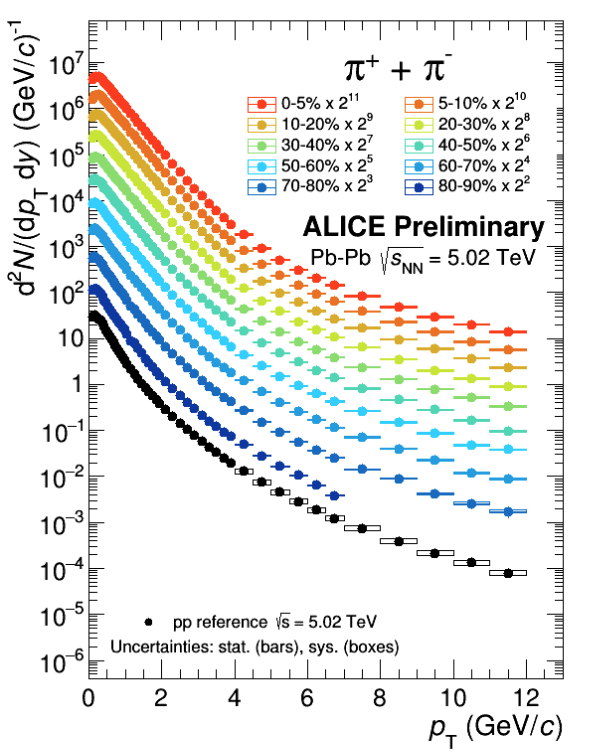
\includegraphics[height=7cm]{FigCap1/PionsPbPb5TeV.png}
   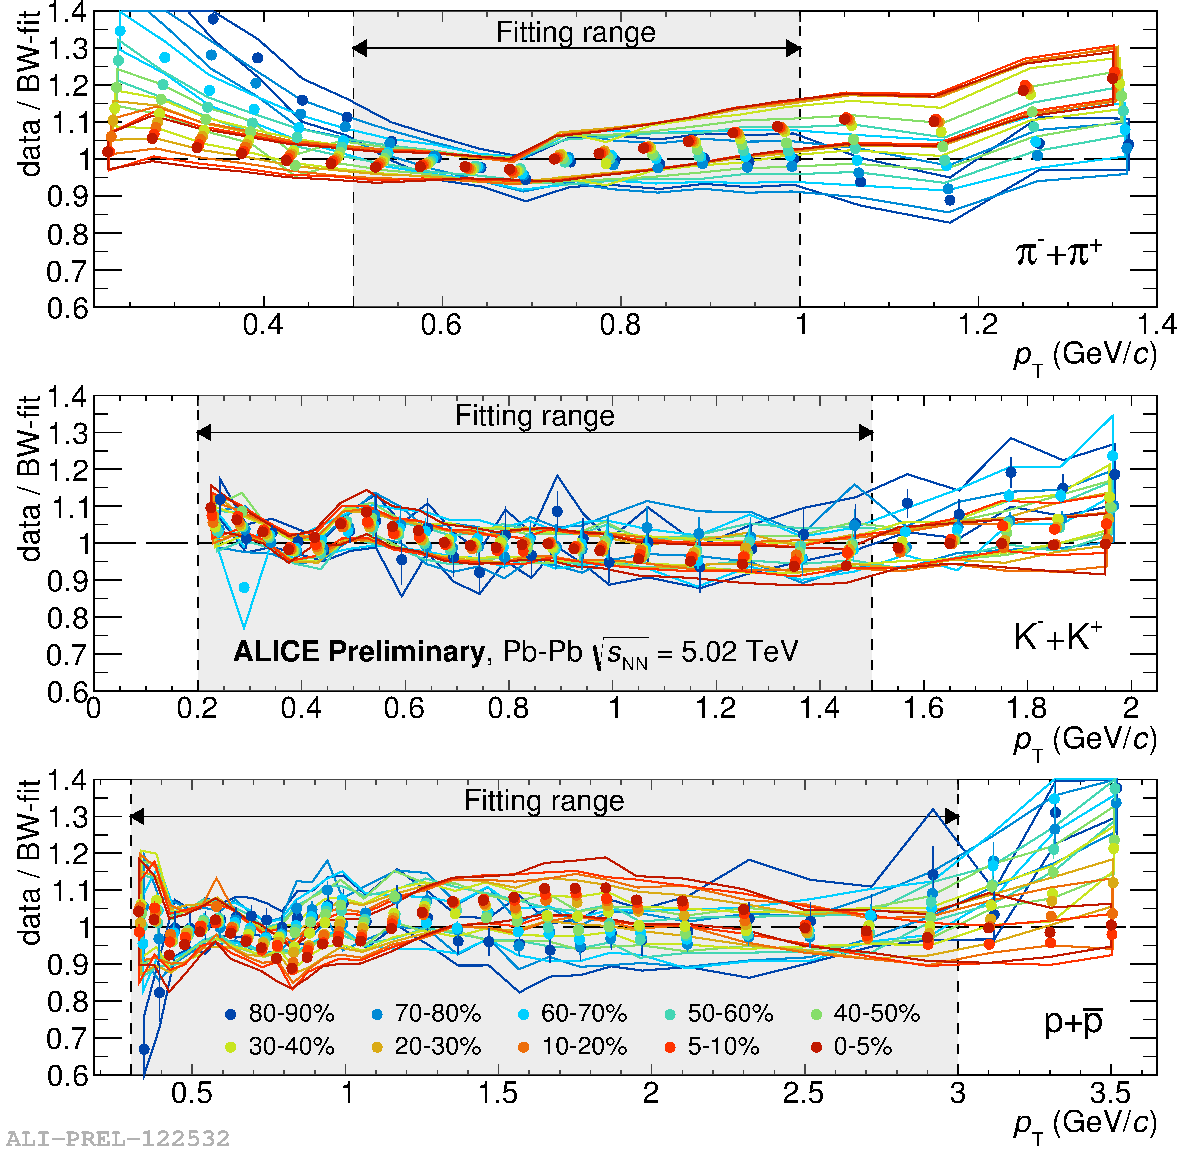
\includegraphics[height=8cm]{FigCap1/BW_5TeV.pdf}
 \caption{Ratio data to blast-wave fit for $\pi, k, p$ spectra as a function of $\pt$ in different centrality classes in Pb-Pb collisions at $\sNN = $ 5.02 TeV~\cite{Jacazio:2017dvy}, measured by ALICE.}
  \label{fig:BWfit}
\end{figure}
\begin{figure}[!t]
  \centering
  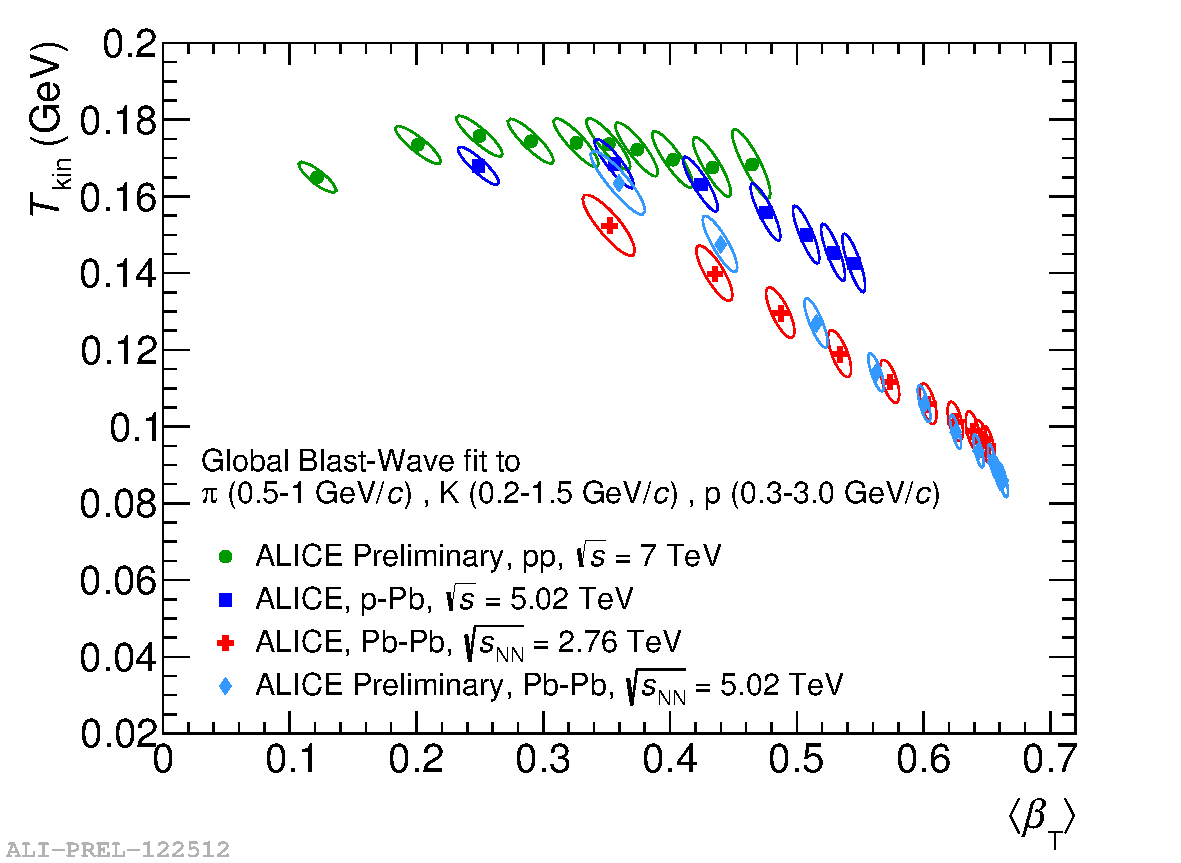
\includegraphics[height=6cm]{FigCap1/BWfit_BetaTplot.pdf}
 \caption{$T_{kin}$ vs $\langle \beta_T \rangle$ from blast-wave fits for different colliding systems and energies~\cite{Jacazio:2017dvy}.}
  \label{fig:BetaTplot}
\end{figure}

The observed particle spectrum results from the sum 
of the spectra of individual thermal sources each boosted with the 
boost angle $\rho = \tanh^{-1}(\beta_{\rm T})$:
\begin{equation}
\label{eq:BlastWave}
\frac{dN}{\pt d\pt d\phi dy}\propto \int_{0}^{R} r dr\;  m_{T}\;  K_{1} \; (\frac{m_{T} \cosh(\rho(r))}{T_{fo}})\;  I_{0}\; (\frac{\pt \sinh(\rho(r))}{T_{fo}}).
\end{equation}
It is a three parameter ($T_{fo}, \beta_s, n$) simplified hydrodynamical model.
The blast-wave fit to the measured spectra allows
  an estimate of the kinetic freeze-out temperature $T_{fo}$ and 
  radial velocity $\beta_{\rm T}$. An example of data to blast-wave fit for the 
  measured spectra of pions, kaons and protons in Pb-Pb collisions at $\sNN = $ 5.02 TeV 
   by ALICE is shown in Fig.~\ref{fig:BWfit}, as a function of $\pt$ (different centrality classes 
   are in different colours).
  
Fig.~\ref{fig:BetaTplot} shows the ALICE results 
for the blast-wave parameters for different colliding systems and energies. Blast-wave parameters
  in Pb-Pb collisions at $\sNN = 5.02$ TeV follow the trends with collision centrality observed at
   lower energy ($\sNN = 2.76$ TeV). The largest expansion velocity 
   is for central Pb-Pb collisions, as well as the lowest temperature
    for the kinetic freeze-out.\\

\subsubsection{Anisotropic flow}
\label{sec:AnisotropicFlow}
The anisotropic flow is characteristic of non-central collisions, where the 
finite impact parameter creates a fireball with a geometrical anisotropy. 
Due to particle rescatterings during the system evolution, the initial spatial 
anisotropy is transferred to a final state momentum-space anisotropy. No
 rescatterings during the system evolution or any delays in time of such 
 interactions would lead to no momentum anisotropy in the final state or
  to a decrease in the elliptic flow signal. Hence, the characterization of 
  anisotropic flow is important as it is sensitive to particle interactions very 
  early in the system evolution. Informations of medium properties, such as Equation of 
  State, sound velocity or shear viscosity can be exctracted by a comparison 
  of the measured anisotropic flow and hydrodynamic model calculations.
\begin{figure}[!ht]
  \centering
  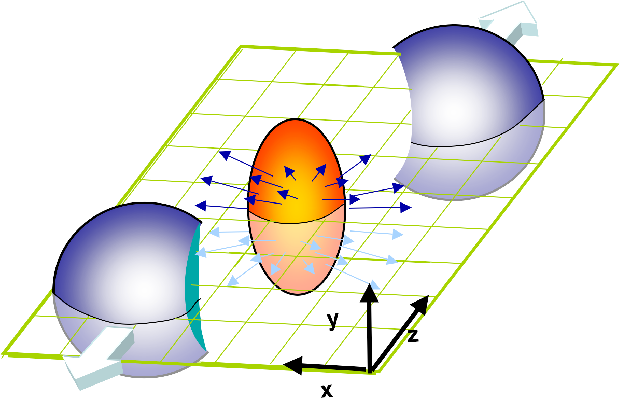
\includegraphics[width=8cm]{FigCap1/elliptic_flow_3D_medium.png}
  \caption{Picture of a semi-peripheral collisions and the pressure gradients arising from a geometrical anisotropy.}
  \label{fig:elliptic_flow_3D_medium}
\end{figure}
In non-central heavy-ion collisions, an almond-shaped interaction 
volume is created (see Fig.~\ref{fig:elliptic_flow_3D_medium}).
The reaction plane is defined by the impact parameter itself and the 
beam line (xz plane in Fig.~\ref{fig:elliptic_flow_3D_medium}). 
A larger pressure gradient in the
 reaction plane than perpendicular to it is expected. This generates an
  anisotropy in azimuthal distributions of the particle momenta with 
  respect to the reaction plane, which can be detected in the measured
   particle azimuthal distributions. This distribution can be parametrized 
   through a Fourier series decomposition:
\begin{equation}
\label{eq:FourierAzimuthExpansion}
E \frac{d^3N}{d^3p} = \frac{1}{2\pi} \frac{d^2N}{\pt d\pt dy} (1 + \sum_{n=1}^\infty 2v_n {\rm cos} (n(\varphi - \Psi_r))),
\end{equation}
where $\varphi$ is the azimuthal direction of the emitted particle and 
$\Psi_r$ denotes the (true) reaction plane angle.
In the formula, {\it v$_n$} are the Fourier coefficients, and they can be 
evaluated as $v_n = \langle cos(n(\varphi - \Psi_r)) \rangle$, where 
$\langle \rangle$ indicates an average over all particles in all events with
 their azimuthal angle $\varphi$ in a given rapidity and $\pt$ momentum at
  a fixed centrality. The sine terms vanish due to the reflection simmetry 
  with respect to the reaction plane. {\it Direct} and {\it elliptic flow} 
  are common terms for the first and the
second order Fourier coefficients respectively in the particle azimuthal 
distribution in Eq.~\ref{eq:FourierAzimuthExpansion}, but coefficients 
up to at least 6th order were measured at the LHC~\cite{ATLAS:2012at}.
With the large amount of data provided by the LHC, in fact, it became accessible
to study not only the on-average anisotropies but the initial space geometries 
fluctuations~\cite{Aad:2013xma,Schukraft:2012ah}, to which first-order and higher-order Fourier 
coefficients were indeed found to be sensitive. 
The positions of the nucleons in the overlap region of the colliding nuclei 
can fluctuate to create matter distributions dipole (n = 1) and
sextupole (n = 3) asymmetries~\cite{Teaney:2010vd,Alver:2010dn,Alver:2010gr}, which are converted into 
non-zero first-order and higher-order harmonic coefficients. 
Fig.~\ref{fig:vnHydro} shows
   comparison to viscous hydrodynamics calculations~\cite{Gale:2012rq} of the 
   Fourier coefficients $v_n$ up to 5$th$ order measured by ATLAS~\cite{ATLAS:2012at}
    (left panel) in Pb-Pb collisions at $\sNN = 2.76$ TeV and 
    PHENIX~\cite{Adare:2011tg} and STAR~\cite{Pandit:2012mq} 
    (right panel) in Au-Au collisions at $\sNN = 200 $ GeV. The value
     of the shear viscosity $\eta/s$ of the medium that allows a good parametrization 
     of hydro calculations for Au-Au collisions at top of RICH energy is 0.12, while the value
      for Pb-Pb collisions at the LHC at $\sNN = 2.76$ TeV is 0.2. 
      This reveals a dependence of the shear viscosity on the temperature of the system.
\begin{figure}[!ht]
  \centering
  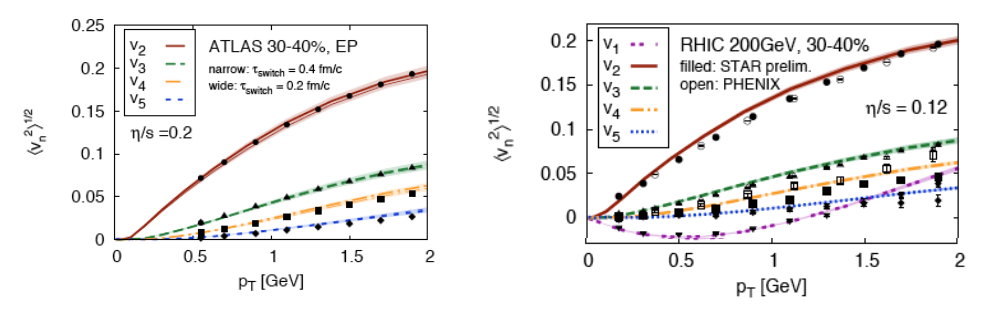
\includegraphics[width=15cm]{FigCap1/RICH_ATLAS_vn.png}
  \caption{Fourier components of anisotropic transverse flow, $v_n(\pt)$, for Pb-Pb collisions at the LHC (left panel) and for Au-Au collisions at RICH (right panel), in comparison with viscous hydrodynamics calculations~\cite{Gale:2012rq}.}
  \label{fig:vnHydro}
\end{figure}
\begin{figure}[!ht]
  \centering
  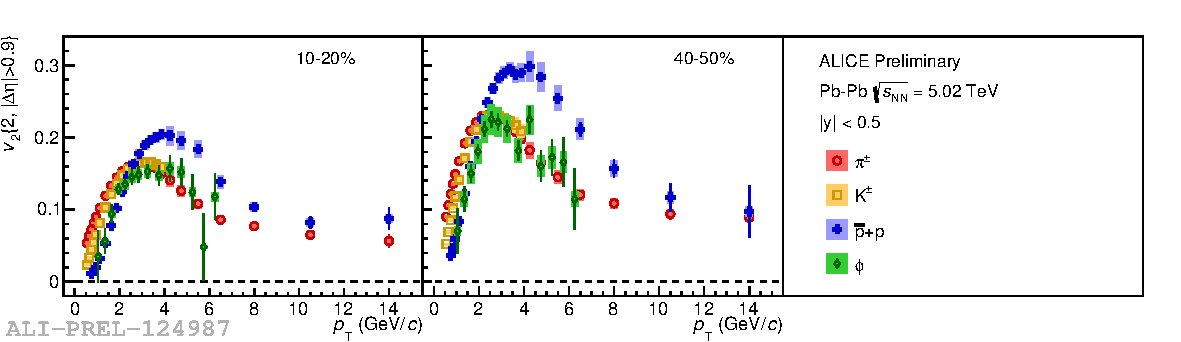
\includegraphics[width=15cm]{FigCap1/v2IdentifiedParticles.pdf}
  \caption{Elliptic flow coefficient $v_2$ of $\pi^{\pm}, K^{\pm}, p(\bar{p})$ and $\Phi$ meson for 10-20\% (left) and 40-50\% (right)
collision centrality as function of $\pt$~\cite{Bertens:2017krr}. Statistical uncertainties are shown as bars and systematic uncertainties as boxes.}
  \label{fig:v2IdentifiedParticles}
\end{figure}
Fig.~\ref{fig:v2IdentifiedParticles} shows the $\pt$-differential 
$v_2$ of $\pi^{\pm}, K^{\pm}, p(\bar{p})$ and $\Phi$ mesons for 10-20\% (left)
and 40-50\% (right) collision centrality~\cite{Bertens:2017krr}, measured by 
ALICE~\cite{Bertens:2017krr} in Pb-Pb collisions at $\sNN = 5.02$ TeV.
For $\pt < 2$ $\Gevc$, one can notice that the $v_2$ of the different species
 follows a mass ordering, which is expected for a hydrodynamically expanding 
 source and is indicative of collective radial flow.
For 3 $< \pt < 8$ $\Gevc$, particles are grouped according to their valence
 quarks, which supports the
hypothesis of particle production via quark coalescence~\cite{Molnar:2003ff}. 
The non-zero $v_2$ at high $\pt$ is attributed to path-length dependent 
in-medium energy loss which is discussed in the next section~\cite{Gyulassy:2000gk}. The $\Phi$ meson, 
with its mass close to proton mass, is a very good probe of quark scaling and 
mass ordering. Indeed, the $\Phi$-meson $v_2$ follows proton $v_2$ at low 
$\pt$, but pion $v_2$ at intermediate $\pt$. \\

\label{sec:ChiralSymm}
\begin{figure}[!ht]
  \centering
  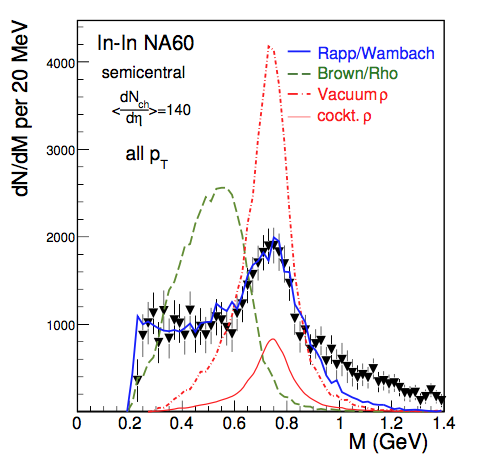
\includegraphics[width=7.2cm]{FigCap1/rhoMelting.png}
  \caption{Di-muon pair invariant mass distribution after 
background subtraction to the $\rho$ meson peak, for In-In collisions at d$N_{ch}$/d$\eta$ = 140, compared to model predictions~\cite{Rapp:2012zq}.}
  \label{fig:JPsiSuppressionNA50}
\end{figure}
\subsection{Chiral symmetry restoration}
If, on one side, chiral symmetry restoration should play a role in the 
observed strangeness enhancement (see Sec.~\ref{subsec:StrangEnhancSPS}),
on the other hand, signatures of this effect could also be found in the line shape of the
invariant mass distribution of thermal low-mass ($< 1$ GeV) dileptons.
Their production is in fact largely carried by light 
vector mesons $\rho, \omega$ and $\phi$. For this reason their are ideal to investigate
changes in the vector-meson mass distributions as the critical temperature for chiral
restoration is approached and surpassed. Changes both in width and in mass of
the mesons were originally advocated as signatures of the chiral transition~\cite{Pisarski:1981mq}. 
Among light vector mesons, the $\rho$ meson was used from the very beginning as the test particle for in-medium 
modifications, due to the abundant production
of $\pi^+ \pi^- \rightarrow \rho$ and subsequent decay $\rho \rightarrow \mu^+ \mu^- $ 
with a lifetime of 1.3 fm/c, shorter than the time between hadronization and the thermal freeze-out. 
Fig.~\ref{fig:JPsiSuppressionNA50} (right) shows NA60 measurement of the 
low-mass di-muon pair invariant mass distribution after 
subtracting the background to the $\rho$ meson peak, 
measured in In-In collisions at top SPS energy~\cite{Damjanovic:2005ni}. The $\rho$ meson is
clearly broadened in the medium as compared to the vacuum case, 
while no sign of mass shift is observed. The measurement
was found to be in good agreement with models describing an in-medium broadening 
scenario (Rapp/Wambach~\cite{Rapp:2012zq}).

\subsection{Jet quenching}
\label{sec:JetQuenching}
Partons produced in the hard scattering processes occurring in the early stages of the 
collisions fragment into collimated cascades of hadrons, that are called jets. 
In heavy-ion collisions partons propagate inside the hot and dense QGP,
 and lose energy because of interactions with the colored medium 
 (jet quenching), primarily via gluon radiation and, to smaller extent, 
 elastic scattering~\cite{Qin:2015srf}. The energy loss ($\Delta E$) carries 
 important information about transport coefficients 
 of the QGP (different for radiative or collisional processes), because it
  is expected to be dependent on the opacity 
 (associated to the medium density and the interaction strength) 
 and on the path length $L$ traversed by the parton inside the medium.
  Different models predict linear and quadratic dependences on $L$ 
  of the energy loss for elastic~\cite{Thoma:1990fm} and radiative~\cite{Baier:1996sk} 
  collisions respectively (a cubic dependence is predicted within the 
  AdS/CFT framework). Furthermore, $\Delta E$ also depends on the 
  color charge (different for quarks and gluons) and on the quark mass, 
  as it will be discussed in Sec.~\ref{sec:HFEnLossinAA} focusing in more detail on the heavy flavour quarks.

\begin{figure}[!ht]
  \centering
  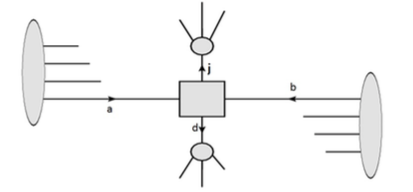
\includegraphics[width=10cm]{FigCap1/Scattering.png}
  \caption{Schematic illustration of high $\pt$ hadron production in high-energy nuclear collisions. }
  \label{fig:Scattering}
\end{figure}

In perturbative QCD, the production cross-section for a hadron $h$ 
from a process involving high-momentum transfer can be described 
using a factorisation approach as a convolution of the incoming parton distribution functions (PDFs) 
inside the nucleons, the hard partonic scattering cross-section and 
the final state fragmentation function (FFs):
\begin{equation}
\label{eq:QCDhardProduction}
\begin{split}
d\sigma_{pp\rightarrow hX} \approx \sum_{abjd}\int dx_a \int dx_b \int dz_j f_{a/p} (x_a, \mu_f) \; \otimes \;f_{b/p} (x_b, \mu_f) \;\otimes \\
d\sigma_{ab \rightarrow jd} (\mu_f,\mu_F,\mu_R) \otimes D_{j\rightarrow h} (z_j,\mu_F), 
\end{split}
\end{equation}
where $x_a$, $x_b$ are the initial nucleon momentum fractions carried by the
 interacting partons, $z_j = p_h/p_j$ is the parton momentum 
 fraction carried by the final observed hadron. Then, $f_{a/p} (x_a, \mu_f)$
  and $f_{b/p} (x_b, \mu_f) $ are the parton distribution functions, 
  $d\sigma_{ab \rightarrow jd} (\mu_f,\mu_F,\mu_R) $ is the differential 
  cross-section for parton scattering process and $D_{j\rightarrow h} (z_j,\mu_F)$
   is the fragmentation function for parton $j$ to hadron $h$, which represents
    the probability for a parton to hadronize into a hadron carrying a fraction $z$ 
    of the parton momentum. Finally, $\mu_f$ and $\mu_F$ are the factorisation 
    scales and $\mu_R$ is the renormalisation scale. The PDFs are measured 
    at a given $Q^2$ in experiments of deep inelastic scattering and evolved
     to different energy scales using DGLAP equations~\cite{Altarelli:1977zs}.
      Fragmentation functions cannot be calculated with pQCD and are usually 
      tuned on measurement in $e^+e^-$ collisions.\\

One of the experimental observables used for the study of energy loss
 inside the QGP is the nuclear modification factor, defined as the ratio 
 between the production of particles in nucleus-nucleus collisions and 
 the one expected according to the binary scaling in nucleon-nucleon collisions:
\begin{equation}
\label{eq:Raa}
\Raa (\pt, y) = \frac{1}{N_{\rm coll}}\frac{d^2N_{\rm AA}/\pt dy}{d^2N_{\rm pp}/\pt dy},
\end{equation}
where $N_{\rm coll}$ is the number of nucleon-nucleon collisions occurring
in the nucleus-nucleus interactions. $\Raa$ is expected to be compatible 
with unity if no medium effects are present. A measurement significantly 
different from the unity implies modifications of the transverse momentum 
distributions of the produced hadrons, that can be related to in-medium 
energy loss effects of quarks.\\


When studying the energy loss of partons inside the QGP, based on
measurements of modification of momentum (energy) distribution of hadrons (jets)
in A-A collisions relative to pp interactions, one 
has to disentangle different effects. The first is that the PDFs of 
bounded nucleons are different from those of the free nucleons. In addition, 
other cold nuclear matter (CNM) effects could affect the measured distributions,
such as $k_{\rm T}$ broadening due to multiple scattering of the
parton in the nucleus or to the hard scattering, energy loss in CNM ... 
Finally, the parton travelling 
  across the QGP experiences energy loss (hot nuclear matter effects) 
  before fragmenting in the final state. Thus taking into account both cold and hot nuclear matter effects, 
Eq.~\ref{eq:QCDhardProduction} becomes:
\begin{equation}
\label{eq:QCDwNuclEffects}
d\sigma_{AB\rightarrow hX} \approx \sum_{abjj\prime d} f_{a/A} (x_a) \; \otimes \;f_{b/B} (x_b) \;\otimes d\sigma_{ab\rightarrow jd} \otimes P_{j\rightarrow j\prime} \otimes D_{h/j\prime}(z_{j\prime}), 
\end{equation}
where the additional piece $P_{j\rightarrow j\prime}$ describes the 
effects of the hard parton $j$ interacting with the colored medium 
before fragmenting into hadrons. \\

It is necessary to disentangle between cold and hot nuclear matter 
effects to have access to the medium transport properties via
 measurements of the $\Raa$. Some of the measurements of $\Raa$
  of high-$\pt$ hadrons and jets at the LHC are presented below.

\subsubsection{High-$\pt$ hadrons}
Measurements of the nuclear modification factors in central heavy-ion 
collisions at four different center-of-mass energies, for neutral pions 
($\pi^0$) (SPS~\cite{Aggarwal:2001gn,dEnterria:2004cly,Alt:2007cd},
 RHIC~\cite{Adare:2012wg}),
 charged hadrons ($h^{\pm}$) (RHIC\cite{Adams:2003kv}), and
  charged particles (LHC~\cite{Abelev:2012hxa,Aad:2015wga,CMS:2012aa}),
   compared to predictions of two models from~\cite{Chien:2015vja,Xu:2015bbz}
    are presented in Fig.~\ref{fig:CMSRaa}. The LHC measurements at
     $\sNN = 2.76$ and 5.02 TeV show stronger suppression than SPS 
     and RHIC measurements. CMS extended the measurement of the 
     $\Raa$ up to 300 $\Gevc$, and the suppression in the high-$\pt$ 
     region is found to be smaller with increasing $\pt$, demonstrating 
     that even very energetic partons suffer energy loss in the medium.
      ALICE complements the picture down to $\pt = 0 \; \Gevc$, 
      showing a perfect agreement with CMS and ATLAS in the medium-$\pt$ region.
\begin{figure}[!ht]
  \centering
  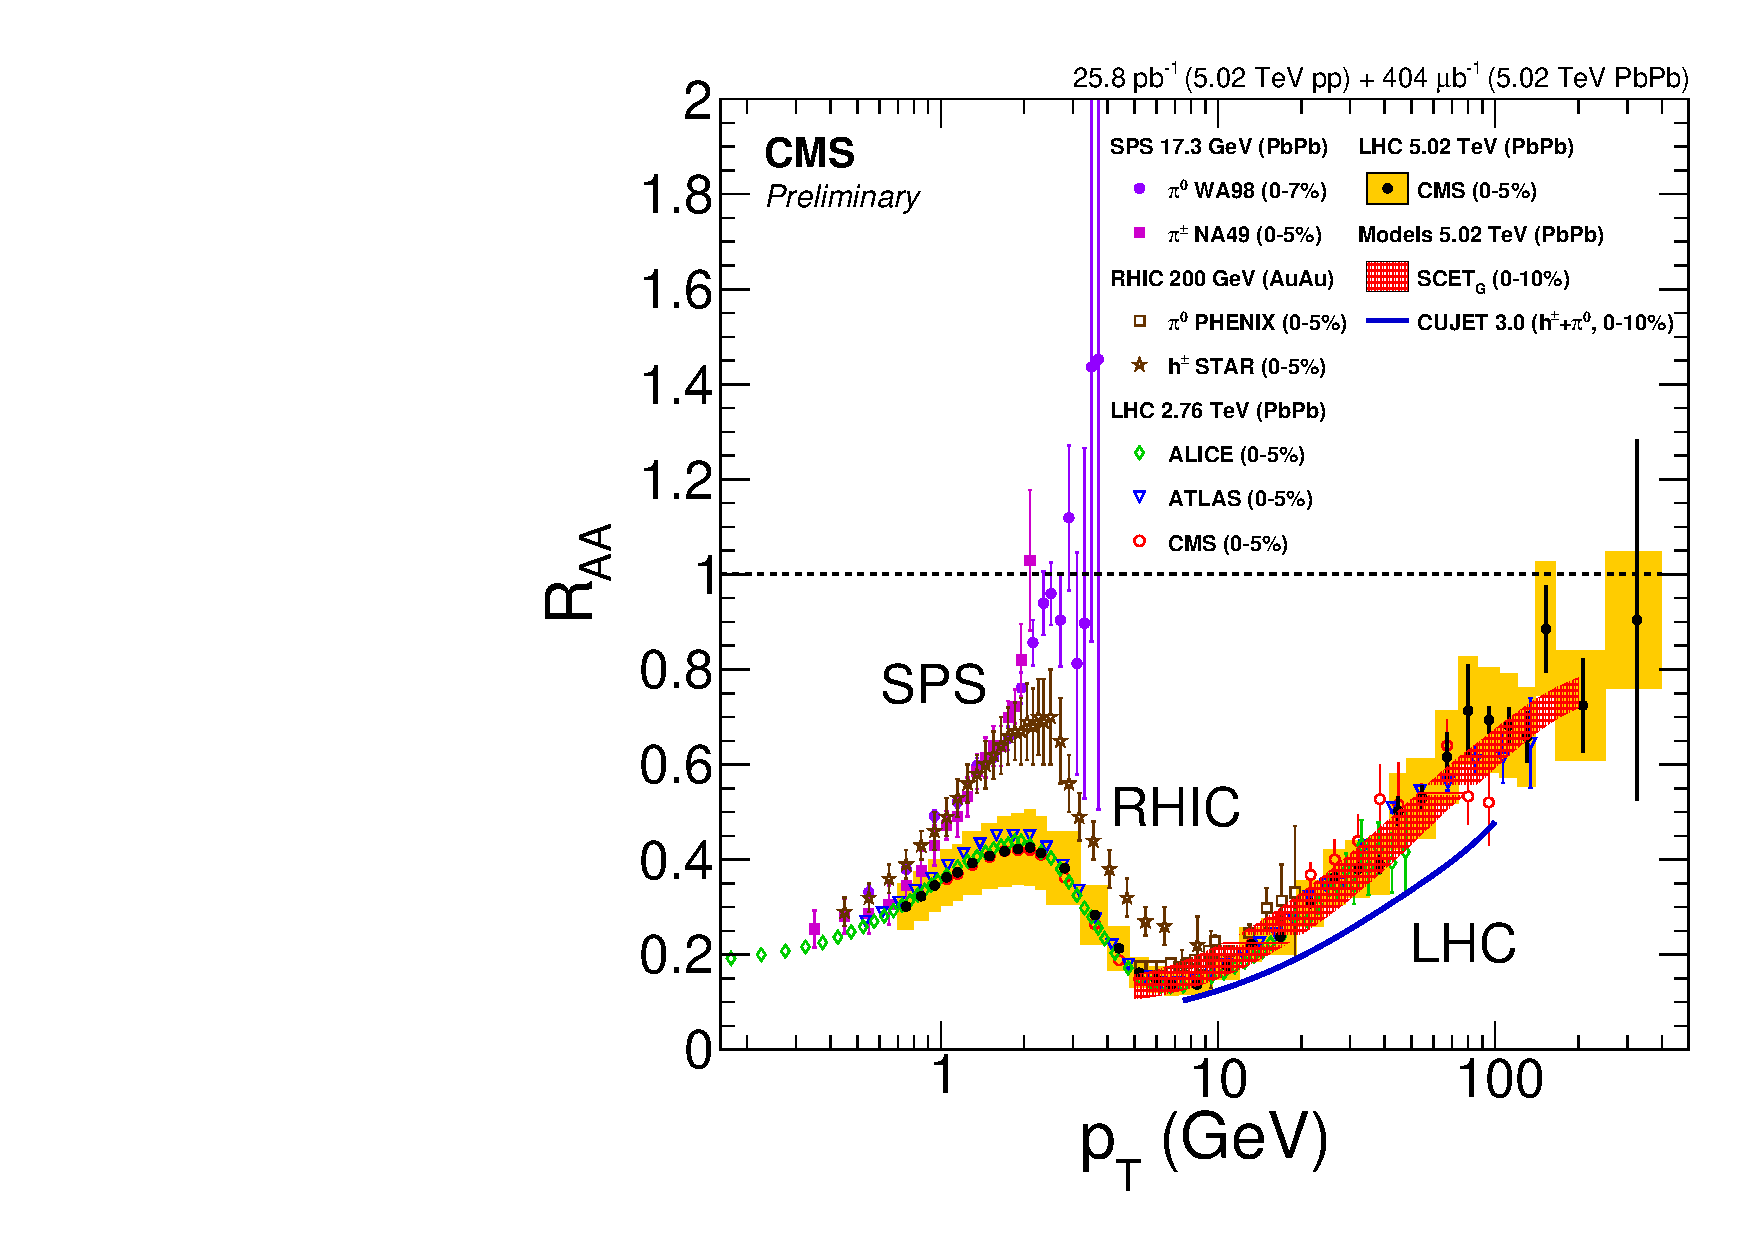
\includegraphics[width=8cm]{FigCap1/CMSRaa.pdf}
  \caption{Measurements of the nuclear modification factors in central heavy-ion collisions at four different center-of-mass energies at SPS~\cite{Aggarwal:2001gn,dEnterria:2004cly,Alt:2007cd}, RHIC~\cite{Adare:2012wg,Adams:2003kv}, and LHC~\cite{Abelev:2012hxa,Aad:2015wga,CMS:2012aa}, compared to predictions of two models from~\cite{Chien:2015vja,Xu:2015bbz}}
  \label{fig:CMSRaa}
\end{figure}
ALICE also measured the nuclear modification factor of identified 
particle species, that can further constrain the models. In Fig.~\ref{fig:PiKPRaa5TeV}
 the $\Raa$ of pions, kaons and protons measured in Pb-Pb collisions 
 at $\sNN = 5.02$ TeV is shown, for different centrality classes. First, it 
 has to be noticed that the suppression has a clear dependence on the 
 collision centrality, since it becomes stronger in more central events, 
 where the medium is more spatially extended, hotter and denser. 
 A second observation from 
  results in Fig.~\ref{fig:PiKPRaa5TeV} is that there is a mass ordering at 
  low $\pt$ that is a direct consequence of the radial flow. In the low-$\pt$
  region, the particle yields in A-A collisions are not governed by the $N_{coll}$ scaling 
  of the yields in pp collisions and the particle spectra are harder in A-A than in pp collisions due to the radial flow. 
  The latter is present at all centralities, but is stronger for central collisions and
  is more pronounced for massive particles.
  
  At high $\pt$
   instead, the suppression is similar for the three species, indicating
    that the medium at high $\pt$ affects the fragmentation of partons in a similar 
    way. Different model calculations were compared to the $\Raa$ 
    measured in different centrality classes by CMS~\cite{CMS:2012aa} 
    and ALICE~\cite{Abelev:2012hxa} and allowed for an extraction of 
    the transport coefficient~\cite{Baier:1996sk} $\hat{q} \approx 1.7-1.9$ 
    GeV$^2/c$ illustrated in~\cite{Burke:2013yra,Liu:2015vna}. 
\begin{figure}[!ht]
  \centering
  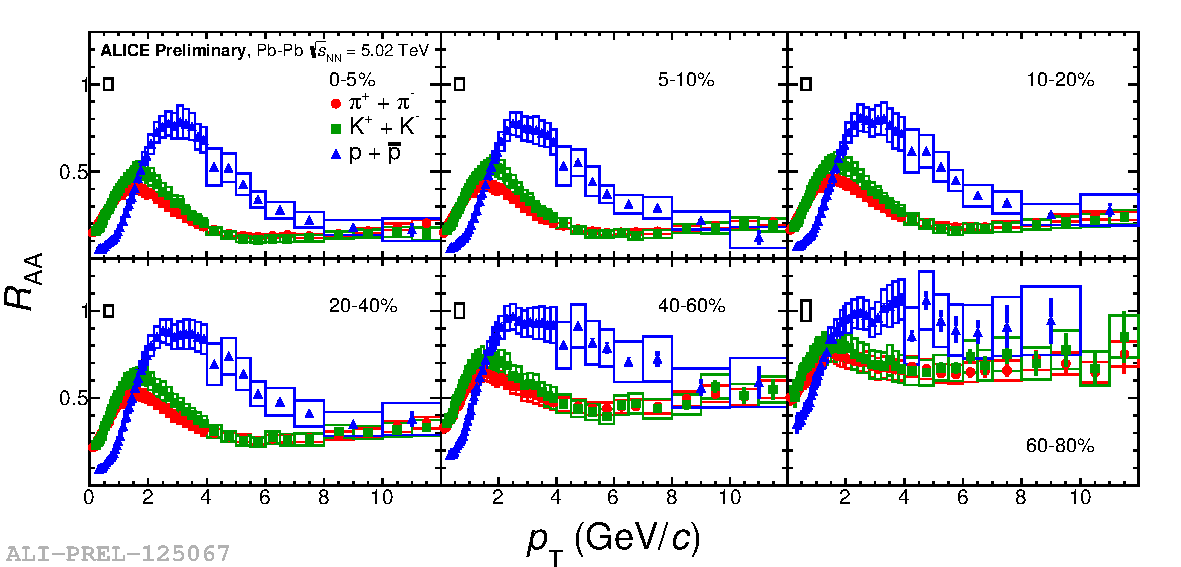
\includegraphics[width=15cm]{FigCap1/KPiPRAA5TeV.pdf}
  \caption{Nuclear modification factor of pions, kaons and protons measured by ALICE in Pb-Pb collisions at $\sNN = 5.02$ TeV in different centrality classes~\cite{Jacazio:2017dvy}.}
  \label{fig:PiKPRaa5TeV}
\end{figure}

\subsubsection{Jets}
The interest in jet measurement with respect to single hadrons is that
the kinematics of the leading parton becomes accessible and we are 
less sensitive to fragmentation effects. Therefore jets are expected to put 
more stringent constraints on assumptions in models for parton energy loss. 
Experimental techniques are now able enough to clearly identify jets 
even in the huge background of high-energy heavy-ion collisions. 
The interaction of the high-$\pt$ partons with the color field of the medium
 induces the radiation of (mostly) soft ($\omega \ll E_{L}$, $E_L$ being the 
 energy of leading parton) and collinear ($k_{\perp} \ll \omega$, $k_{\perp}$ being
 the transverse component of the radiated gluon momentum) gluons. The 
 modeling of a jet emerging from the medium is more complex than that of
  single hadron, since not only the energy loss of the leading parton has to be 
  kept into account, but also the radiated gluons can further re-scatter in the 
  medium inside the jet cone. Thus the total energy inside the jet cone 
  of radius $R$ at the time $t_f$ is:
\begin{equation}
\label{eq:EnergyJet}
E_{jet}(t_f,R) = E_L(t_f) +E_g(t_f,R),
\end{equation}
where $E_g$ is the energy of the radiated gluons, that is defined as:
\begin{equation}
\label{eq:Eg}
E_g(t_f,R) = \int_R d\omega dk^2_\perp \omega f_g(\omega,k^2_\perp,t_f),
\end{equation}
where $f_g(\omega,k_{\perp},t)$ is the double differential distribution of 
the accompanying gluons of the leading parton. It can be obtained after solving 
the following transport equation for the distribution of radiated gluons:
\begin{equation}
\label{eq:RadGluonTransport}
\frac{df_g(w,k_{\perp},t)}{dt} = -\hat{e}\frac{\partial f_g}{\partial \omega} + \frac{1}{4}\hat{q}\nabla^2_{k_{\perp}}f_g + \frac{dN^{rad}_g}{d\omega dk^2_{\perp} dt}.
\end{equation}
The first and the second term in the right-hand side of Eq.~\ref{eq:RadGluonTransport} 
describe the evolution of radiated gluons which can transfer energy 
into the medium via collisional processes (controlled by coefficient 
$\hat{e}$) and accumulate transverse momentum $k_\perp$ 
(coefficient $\hat{q}$). The last term accounts for additional gluon 
radiation coming from emission of the leading parton.\\
\begin{figure}[!ht]
  \centering
  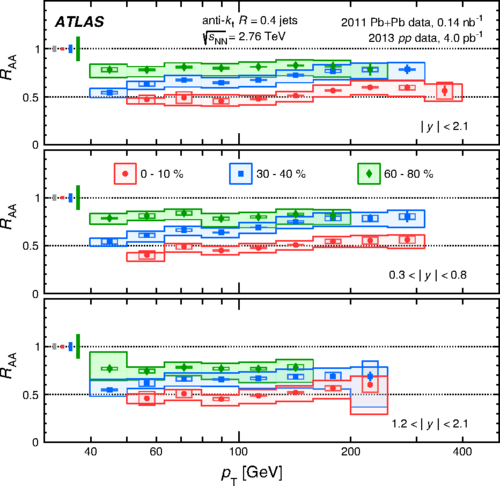
\includegraphics[width=9cm]{FigCap1/ATLASjetsRaa.png}
  \caption{Jet $\RAA$ as a function of $\pt$ in different centrality
intervals in Pb-Pb collisions at $\sNN = 2.76$ TeV~\cite{Aad:2014bxa}. Each panel shows a different range in $|y|$.}
  \label{fig:ATLASjetsRaa}
\end{figure}
\begin{figure}[!ht]
  \centering
  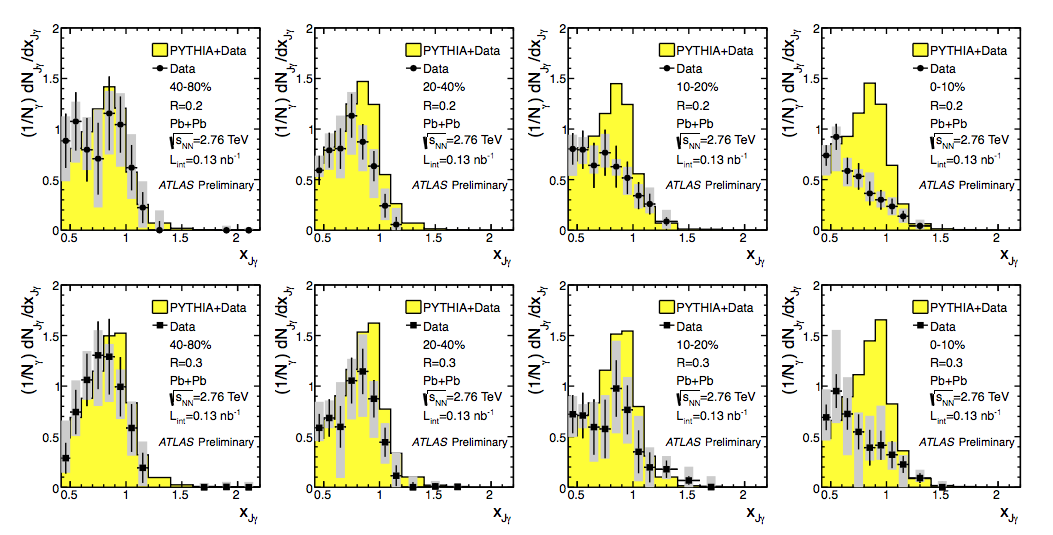
\includegraphics[width=15cm]{FigCap1/ATLASdiijetGammaZ.png}
  \caption{$\frac{1}{N}\frac{dN}{dx_J}$ distribution for reconstructed photon-jet events in Pb-Pb collisions at $\sNN = 2.76$ TeV compared to PYTHIA calculations ($x_J$ is defined in the text)~\cite{ATLAS-CONF-2012-121}. Different centrality classes are shown in each column, while the rows show results for two jet radii, R $= 0.2$ and R $=0.3$.}
  \label{fig:ATLASdijetAsymm}
\end{figure} 
Fig.~\ref{fig:ATLASjetsRaa} shows the jet $\Raa$ measured by ATLAS 
as a function of $\pt$ in different centrality classes and different 
rapidity selections for the three panels~\cite{Aad:2014bxa}. The 
suppression has a clear dependence on the event centrality, while 
is quite flat as a function of $\pt$ in the analysed range from 40 to 400 $\Gevc$. 
This result confirms the strong suppression observed for high-$\pt$ 
charged hadron yield in Pb-Pb relative to pp collisions at LHC energies and reveals that the 
medium is so opaque to quench even the most energetic jets. The 
azimuthal correlations of transverse energy of back-to-back jets 
constitute an other interesting observable to characterize the effect 
of jet-medium interaction. At LHC energies, a large number of dijet 
from back-to-back partons is observed to have an asymmetry in the energy 
of the two reconstructed jets, that can be quantified by 
$x_J = \pt^{jet1}/\pt^{jet2}$. Fig.~\ref{fig:ATLASdijetAsymm} shows the $\frac{1}{N}\frac{dN}{dx_J}$ 
distribution for reconstructed photon-jet events in Pb-Pb collisions at $\sNN = 2.76$ TeV 
compared to PYTHIA calculations~\cite{ATLAS-CONF-2012-121}. 
Each column corresponds to different centrality classes, while the 
rows show results for two jet radii, R $= 0.2$ and R $=0.3$. In more 
peripheral collisions the $x_J$ distribution is peaked towards 1, thus 
meaning that higher $\pt$ dijets tend to be balanced in momentum. 
Moving towards more central events, the $x_J$ distribution appears 
flatter around $0.5 < x_J<1$, to eventually become peaked around 
$x_J \sim 0.5$ in the 10\% more central events.
This is understood in terms of different path 
lengths that the two partons have to traverse in the medium. In general, 
measurements of inclusive jets and dijet suffer from the fact that leading jets 
experience themselves some energy loss, thus the energy of the jet is not 
fully defined. Using weak bosons (Z or W) or photons, that do not interact 
with the medium, to replace one of the two jets allows us to fully calibrate the 
initial energy of the jet, as explained in~\cite{Wang:1996yh}. 

% \begin{figure}[!ht]
%   \centering
%   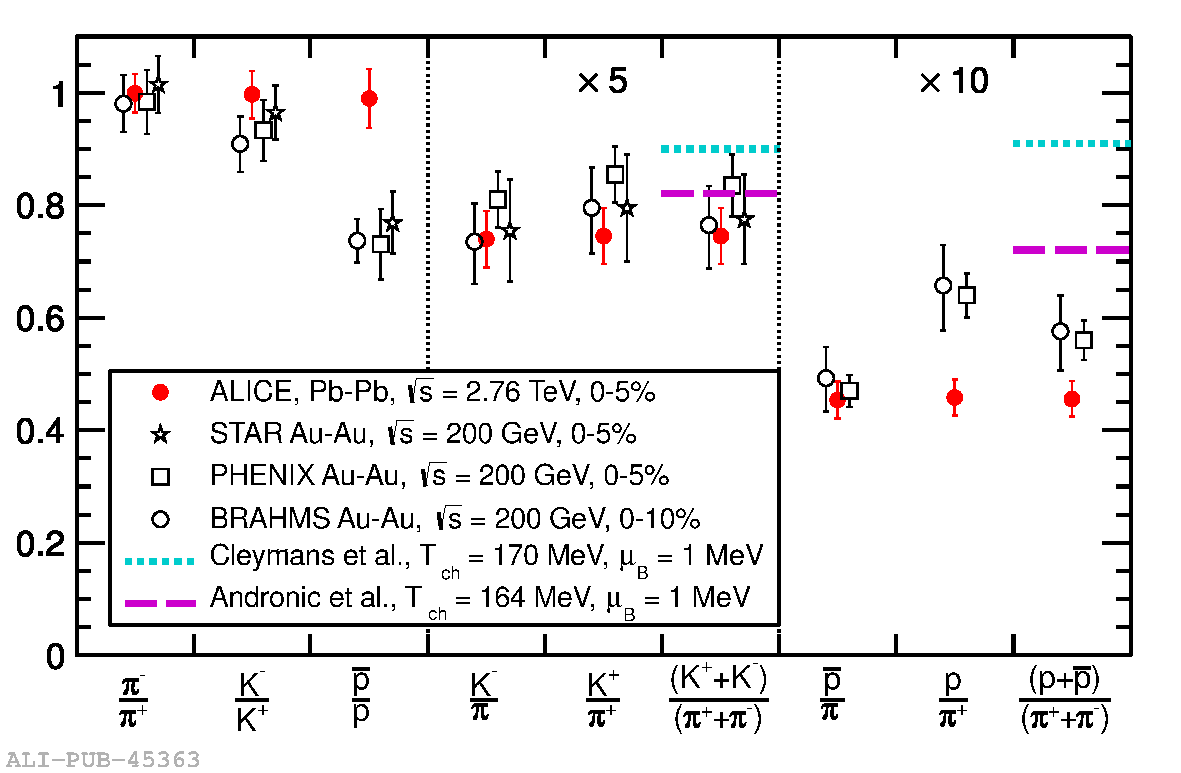
\includegraphics[width=10cm]{FigCap1/CentralPbPbRatiosThermalModels.pdf}
%   \caption{Mid-rapidity particle ratios, compared to RHIC results~\cite{Abelev:2008ab,Adler:2003cb,Arsene:2005mr} and predictions from thermal models~\cite{Andronic:2008gu,Cleymans:2006xj} for central Pb-Pb collisions at the LHC (combined statistical and systematic errors)~\cite{Abelev:2012wca}. }
%   \label{fig:CentralPbPbRatiosThermalModels}
% \end{figure}
\subsection{Quarkonium production}
\label{sec:Quarkonium}
Quarkonium, the bound state of a $c\bar{c}$ (charmonium) or $b\bar{b}$ 
(bottomonium) pair, was proposed from the very beginning as one of the 
most powerful signatures of the QGP formation.
The signature given by the J/$\psi$ vector meson yield is of particular interest
in the view of assessing about the formation of a deconfined medium.
The J/$\psi$ mesons, and more in general the charmonium states, are formed 
by a $c\bar{c}$ quark pair, that can only be produced (due to the large mass) 
in the initial hard parton scatterings, occurring before the formation of the 
Quark-Gluon Plasma. Theoretical calculations based on lattice QCD 
predict a J/$\psi$ suppression to be induced by the screening of the color 
force in a deconfined medium, due to the presence of free 
color charges, which becomes stronger as the temperature 
increases~\cite{Abreu:2000ni,Matsui:1986dk}. 
J/$\psi$ suppression was first observed at the SPS in Pb-Pb collisions, by 
the NA38 and NA50 experiments~\cite{Abreu:2000ni}.
The ratios between the observed J/$\psi$ yield and the expected one 
based on the so-called ``ordinary nuclear absorption" measured in p-A 
collisions are shown in Fig.~\ref{fig:JPsiSuppressionNA50} 
as a function of the energy density $\epsilon$ of the medium traversed by the charmonium state. 
The results showed that for energy densities up to $\epsilon \lesssim 2.5$ GeV/fm$^3$, 
the yield of the J/$\psi$ meson is compatible with measurements in pp 
and p-A collisions, in which only ordinary nuclear absorption is present. In Pb-Pb 
collisions, instead, where $\epsilon$ becomes larger, there is a clear deviation from 
unity of the ratio measured/expected, which was interpreted as a first indication of 
charmonium suppression due to colour screening in the QGP.
\begin{figure}[!ht]
  \centering
  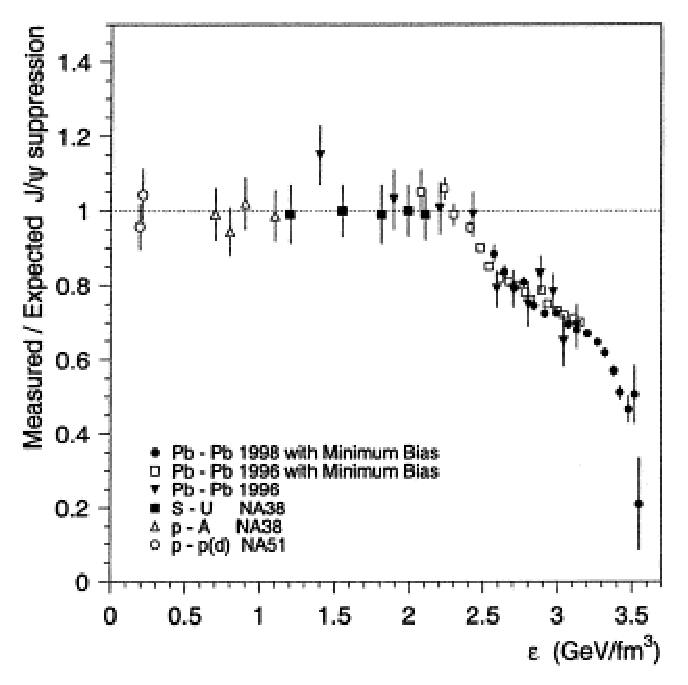
\includegraphics[width=6.6cm]{FigCap1/JPsiSuppressionNA50.eps}
  \caption{Ratio between measured J/$\psi$ production and expected one in pp, p-A and A-A collisions as function of the energy density of the medium ~\cite{Abreu:2000ni}.}
  \label{fig:JPsiSuppressionNA50}
\end{figure}
Clear signs of J$/\psi$ suppression were indeed measured at the SPS, as a 
consequence of the strong color field of the plasma~\cite{Abreu:2000ni}. 
Charmonium states were also expected to melt at different temperatures of 
the plasma, accordingly to their binding energy, giving rise to a sequential melting 
scenario~\cite{Du:2015wha,Digal:2001ue}. What turned 
out to be unexpected when data at higher collision energies became available 
was that the RICH~\cite{Adare:2011yf,Adare:2006ns} J$/\psi$ suppression 
had the same magnitude as the one observed at the SPS~\cite{Scomparin:2007rt}.
At LHC energies, a reduced suppression as compared to lower
collision energies was observed~\cite{Abelev:2013ila}.
In Fig.~\ref{fig:RaaJPsi} the ALICE measurements 
of J$/\psi$ $\Raa$ in Pb-Pb collisions at $\sNN = 2.76$ TeV~\cite{Abelev:2013ila} 
and at $\sNN = 5.02$ TeV~\cite{Adam:2016rdg} are compared to measurements at 
RHIC~\cite{Adare:2011yf} for Au-Au collisions at $\sNN = 200$ GeV. In the left panel of Fig.~\ref{fig:RaaJPsi} 
the $\Raa$ is presented as a function of the centrality and shows smaller J$/\psi$ suppression 
at the higher energies, where the measurement is for J$/\psi$ with $\pt < 8 \Gevc$. 
The centrality dependence is similar at the two LHC energies. 
In the right panel of the same figure, the 
dependence on $\pt$ reveals that the different suppression at different $\sNN$ is mostly
in the low-$\pt$ region.
CMS measured the J$/\psi$ $\Raa$ 
in the high $\pt$ region, up to $\pt = $ 30 $\Gevc$, confirming a stronger suppression
($\RAA \approx 0.3$ for most central events) with respect to 
low $\pt$~\cite{Khachatryan:2016ypw}. All these observations can be 
explained by a (re)generation effect of uncorrelated $c$ and $\bar{c}$ quarks, relevant at LHC energies due to the 
large production cross-section of $c\bar{c}$ quark pairs. 
An other observable that is sensitive to the J$/\psi$ production 
mechanism is the elliptic flow $v_2$. If the J$/\psi$ is produced by coalescence 
of charm quarks, and the charm thermalises in the medium, the J$/\psi$ 
should inherit the flow of the quarks and show a positive $v_2$. 
A non-zero $v_2$ could also be observed due to the path-length dependence of charmonium
in-medium energy loss, thus the final $v_2$ may be an 
interplay of multiple effects. Fig.~\ref{fig:JPsi} presents recent measurements 
by ALICE of J$/\psi$ $v_2$ at forward and mid-rapidity in Pb-Pb collisions at 
$\sNN = 5.02$ TeV for semi-central events (20-40\% centrality class)~\cite{Acharya:2017tgv}, 
compared with some of the available theoretical models. At forward rapidity, 
the maximum $v_2$ is reached in $4 < \pt < 6\; \Gevc$, with a 
significance for non-zero $v_2$ larger than $6.6\sigma$. Model calculations 
that include (re)combination of thermalised charm and beauty quarks as 
source of J$/\psi$ production, together with a path-length dependent in-medium 
energy loss can describe the data at low $\pt$, but fail in 
reproducing the measured shape at higher $\pt$, suggesting a missing mechanism in the 
model ({\it Du et al.} in Fig.~\ref{fig:JPsi}~\cite{Du:2015wha}). The model by 
{\it Zhou et al.}~\cite{Zhou:2014kka} includes, in addition to the cited components, 
a contribution from the modification of quarkonium production in the presence 
of a strong magnetic field in the early stage of the heavy-ion collision~\cite{Guo:2015nsa}. 
The $v_2$ resulting from the different in-plane and out-of-plane survival 
probabilities of primordial J$/\psi$ is shown as dashed red and dash-dotted 
orange lines. At LHC energies also the bottomonium states have been 
measured, opening the way to precision studies for the $\Upsilon$({\it n}S) 
family. Due to smaller production cross-section of $b$ quarks compared to $c$ quarks, 
effects of coalescence are
expected to be of smaller impact with respect to charmonium~\cite{Andronic:2015wma}. 
A sequential suppression pattern is expected also for $b\bar{b}$ states, due to 
different binding energies of the bottomonium states. CMS measured 
the $\Raa$ of $\Upsilon$(1S), $\Upsilon$(2S) and $\Upsilon$(3S) as a 
function of the centrality in Pb-Pb collisions at 
$\sNN = 2.76$ TeV~\cite{Khachatryan:2016xxp} (Fig.~\ref{fig:JPsi}, right) and at 
$\sNN = 5.02$ TeV~	\cite{Sirunyan:2017lzi}. The $\RAA$ in the right panel of Fig.~\ref{fig:JPsi} shows a 
suppression for the $\Upsilon$(2S) state (factor of 8), that is larger with 
respect to the $\Upsilon$(1S) state (factor of $\sim$ 2), while for 
the $\Upsilon$(3S) only an upper limit could be determined.
The measured suppression of the three $\Upsilon$ states is compatible 
with theoretical models of a sequential melting of quarkonium states in a 
hot medium~\cite{Khachatryan:2016xxp}.
%~\cite{Sirunyan:2016znt}
\begin{figure}[!ht]
  \centering
  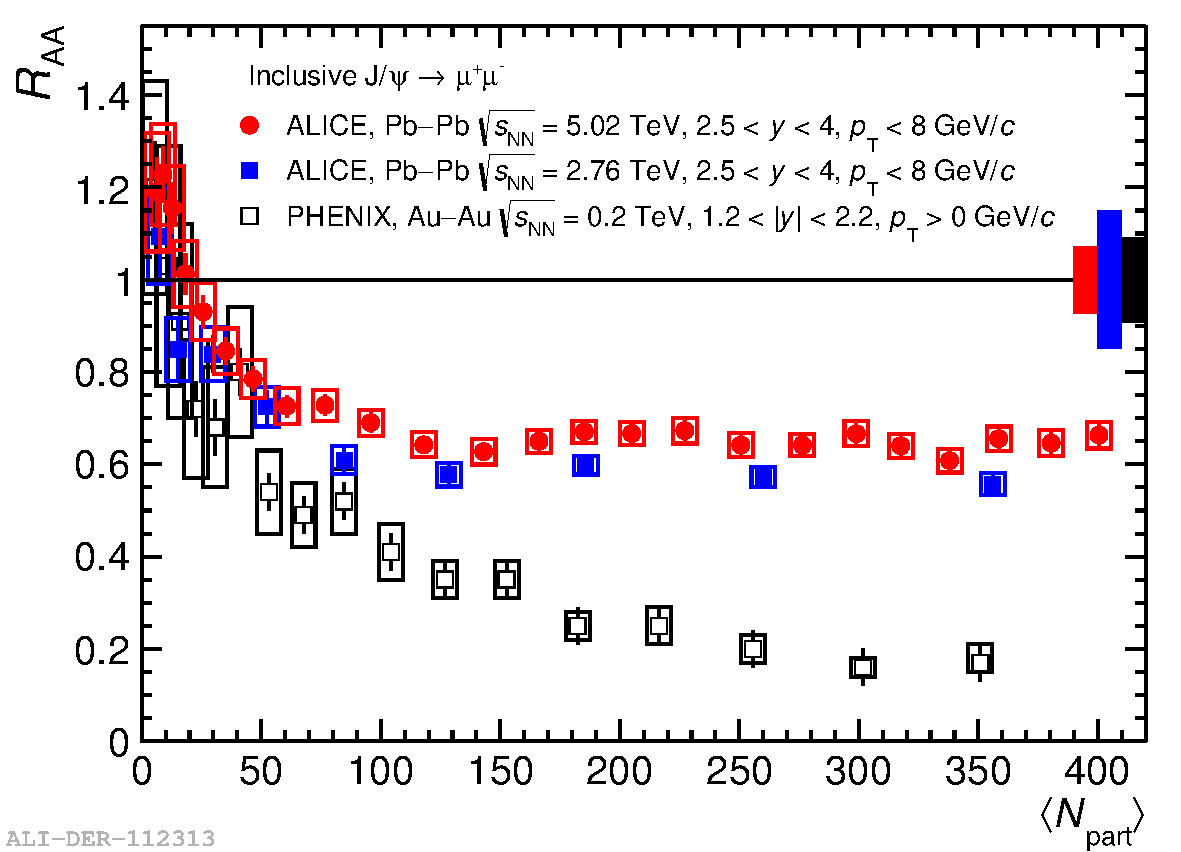
\includegraphics[width=7cm]{FigCap1/RaaJPsiAlicePhenix.pdf}
  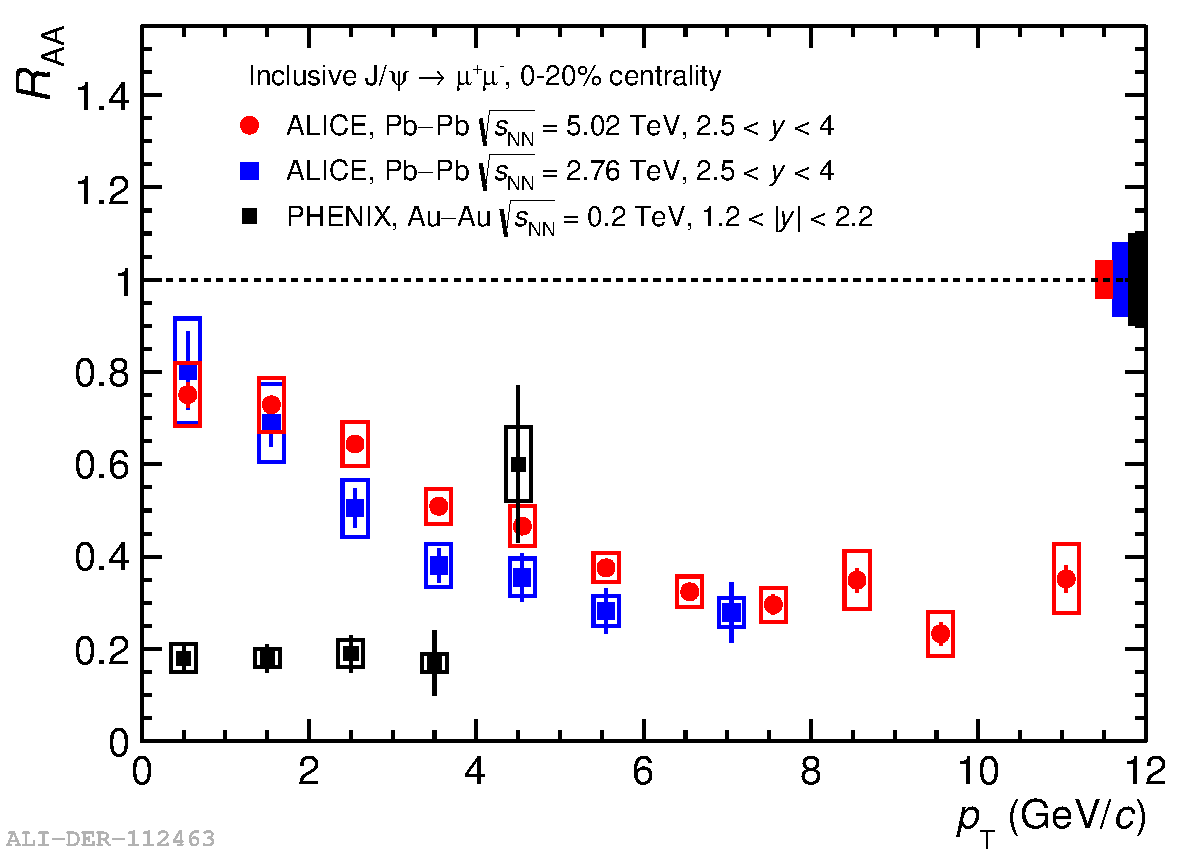
\includegraphics[width=7cm]{FigCap1/RaaJPsiAlicePhenixVsPt.pdf}
  \caption{Centrality (left) and transverse momentum (right) dependence of the J$/\psi$ $\RAA$ measured by ALICE in Pb-Pb collisions at $\sNN = 2.76$ TeV~\cite{Abelev:2013ila} (blue) and at $\sNN = 5.02$ TeV~\cite{Adam:2016rdg} (red) compared to PHENIX~\cite{Adare:2011yf} results Au-Au collisions at $\sNN = 200$ GeV.}
  \label{fig:RaaJPsi}
\end{figure}

\begin{figure}[!ht]
  \centering
  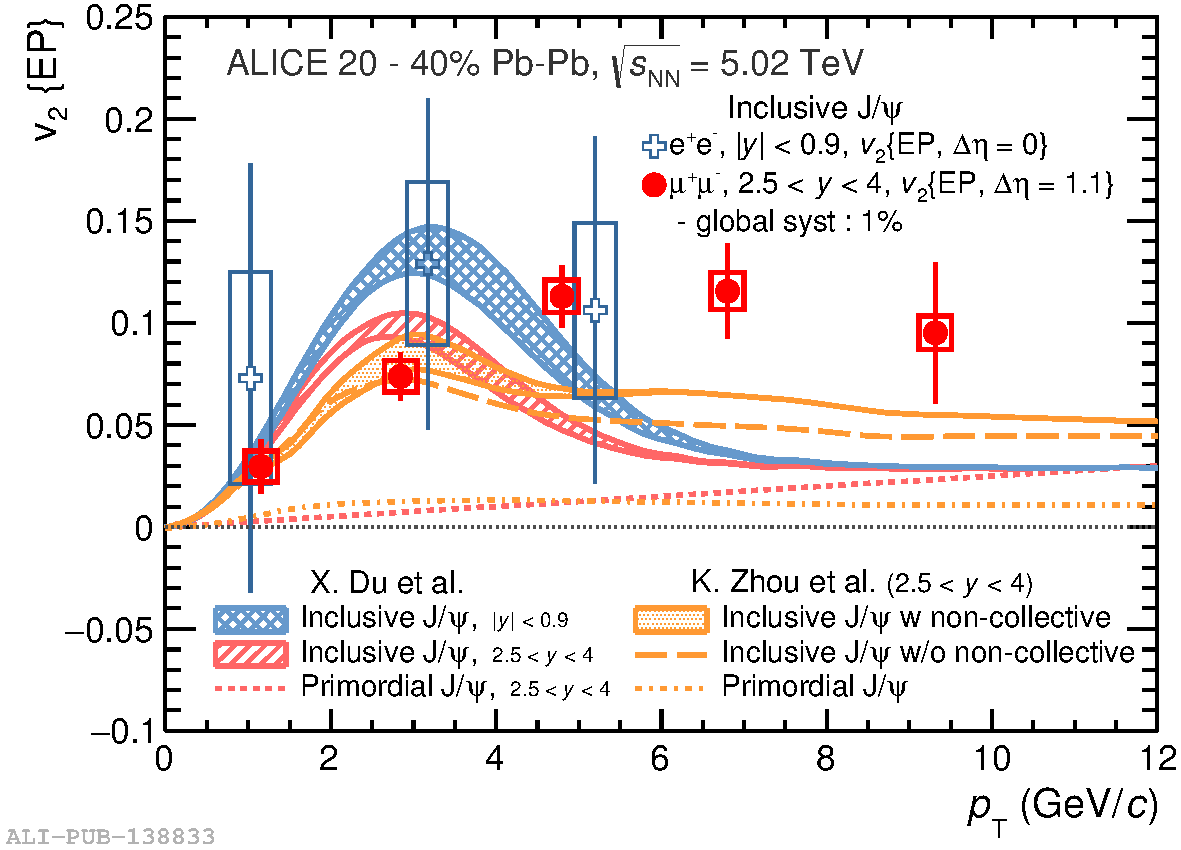
\includegraphics[width=7cm]{FigCap1/JPsiV2Models.pdf}
  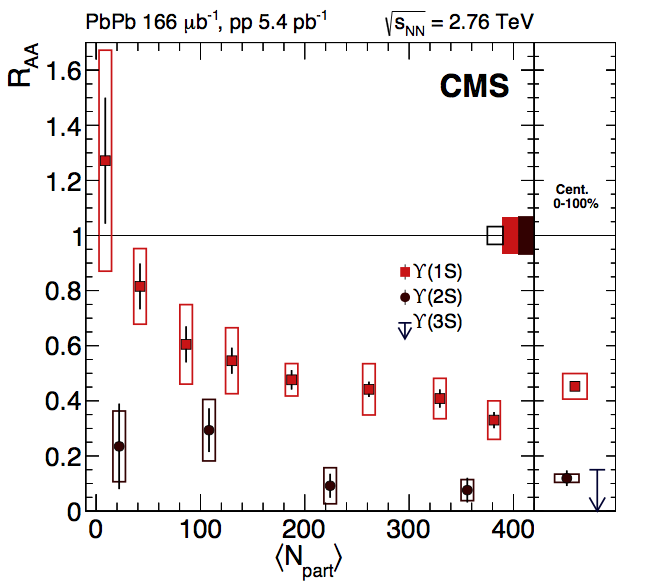
\includegraphics[width=6cm]{FigCap1/RaaUpsilonCMS.png}
  \caption{Left: inclusive J$/\psi$ $v_2(\pt)$ at forward and mid-rapidity for semi-central (20-40\%) Pb-Pb collisions at $\sNN =$ 5.02 TeV~\cite{Acharya:2017tgv}. Calculations from transports model from Refs.~\cite{Du:2015wha} and~\cite{Zhou:2014kka} are also shown. Right: nuclear modification factors of $\Upsilon$(1S) and $\Upsilon$(2S) meson production in Pb-Pb collisions measured by CMS, as a function of centrality.
The upper limit derived on the nuclear modification factor for $\Upsilon$(3S) is represented with an arrow in the centrality integrated panel on the right~\cite{Khachatryan:2016xxp}. }
  \label{fig:JPsi}
\end{figure}

\subsection{Latest discoveries in small systems}
In 2010 CMS discovered first signals of long-range rapidity correlations in 
high-multiplicity pp collisions at $\sqrt{s} = $ 7 TeV~\cite{Khachatryan:2010gv}, an effect that 
resulted quite unexpected to be found in small systems. Such correlations
were already observed in Au-Au collisions at RICH~\cite{Alver:2008aa,Alver:2009id,Abelev:2009jv}
and naturally explained in terms of collective expansion of the medium formed in the collisions.
This observation paved the way to search further signals of collective 
behaviours in small systems. 
The interest in the angular correlations among particles lays in the possibility 
to reveal the underlying mechanisms of particle production. In~\cite{Khachatryan:2010gv}, 
CMS studied the two-dimensional $\Delta \eta$-$\Delta \phi$ correlation 
function, where $\Delta \eta$ is the difference in pseudo-rapidity between 
two particles and $\Delta \phi$ is the difference in their azimuthal angle $\phi$. The $\pt$-inclusive two-particle 
correlation, as a function of $\Delta \eta$ and $\Delta \phi$ is defined as:
\begin{equation}
\label{CorrelationFnc}
R(\Delta \eta,\Delta \phi) = \Big \langle (\langle N \rangle -1) \Big (\frac{S_N(\Delta \eta,\Delta \phi)}{B_N(\Delta \eta,\Delta \phi)} -1\Big )\Big \rangle,
\end{equation}
where (i) $S_N(\Delta \eta,\Delta \phi)$ is the correlation function for the signal distribution,
determined by counting all particle pairs in each event within a multiplicity bin, 
(ii) $B_N(\Delta \eta,\Delta \phi)$ is the correlation function for the background distribution, determined
  by correlating each charged particle of one event with every particle from 
a different event within the same multiplicity bin, (iii) the average is made over all the multiplicity bins of the analysis.
\iffalse
We can define now two correlation functions, the first one, $S_N(\Delta \eta,\Delta \phi)$ for the signal distribution:
\begin{equation}
\label{SignalDistribution}
S_N(\Delta \eta,\Delta \phi) = \frac{1}{N(N-1)}\frac{d^2N^{signal}}{d\Delta \eta d\Delta \phi}
\end{equation}
and the second, $B_N(\Delta \eta,\Delta \phi)$, for the background distribution:
\begin{equation}
\label{BkgDistribution}
B_N(\Delta \eta,\Delta \phi) = \frac{1}{N^2}\frac{d^2N^{mixed}}{d\Delta \eta d\Delta \phi}.
\end{equation}
$S_N(\Delta \eta,\Delta \phi)$ can be determined by counting all particle pairs in each 
event within a multiplicity bin, using the weighting factor $N(N-1)$. $B_N(\Delta \eta,\Delta \phi)$ 
is obtained instead by correlating each charged particle of one event with every particle from 
a different event within the same multiplicity bin. Finally, the $\pt$-inclusive two-particle 
correlation, as a function of $\Delta \eta$ and $\Delta \phi$ is obtained as:
\begin{equation}
\label{CorrelationFnc}
R(\Delta \eta,\Delta \phi) = \Big \langle (\langle N \rangle -1) \Big (\frac{S_N(\Delta \eta,\Delta \phi)}{B_N(\Delta \eta,\Delta \phi)} -1\Big )\Big \rangle,
\end{equation}
where the average is made over all the multiplicity bins of the analysis. 
\fi
By using the ratio of $S_N(\Delta \eta,\Delta \phi)$ and $B_N(\Delta \eta,\Delta \phi)$, 
detector effects such as tracking inefficiencies, non-uniform acceptances, etc, are 
automatically corrected. In Fig.~\ref{fig:CMSLongRangeRidge_pp7TeV}, $R(\Delta \eta,\Delta \phi)$ 
is plotted for high-multiplicity events ($N_{tracks} > 110$) in pp collisions at $\sqrt{s} = $ 7 TeV, 
selecting tracks with $1 <\pt < 3\; \Gevc$. Several correlation structures are present. 
The narrow peak at $(\Delta \eta, \Delta \phi) \approx (0,0)$ is the contribution 
from jet-like particle production (near-side peak). The broad ridge around $\Delta \phi \approx \pi$ 
is due to the fragmentation of back-to-back jets (away-side ridge). The ridge-like 
structure that appears around $\Delta \phi \approx 0$ was unexpected,
 indeed never observed in two-particle correlations in pp data, neither in minimum-bias 
 events nor in high-multiplicity low $\pt$ events. Event generators, such as PYTHIA, did not reproduce the 
 observed structure, that seems to resemble hydrodynamic behaviors of heavy-ion 
 collisions~\cite{Alver:2008aa,Alver:2009id,Abelev:2009jv}, and the physical origin is still not clear.
\begin{figure}[!ht]
  \centering
  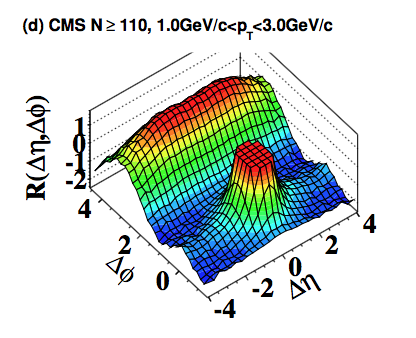
\includegraphics[width=7cm]{FigCap1/CMSLongRangeRidge_pp7TeV.png}
  \caption{Two-particle correlation functions in $\eta$-$\phi$ for 7 TeV pp collisions, in high multiplicity events ($N_{trk}>110$), with 1 $< \pt < 3 \Gevc$~\cite{Khachatryan:2010gv}.}
  \label{fig:CMSLongRangeRidge_pp7TeV}
\end{figure}
From this first observation, many studies have been done to unravel the nature of the 
long-range near side peak. Correlations among several produced particles have been explored, 
since this allows to further suppress short-range particle correlations, 
such as jets or resonance decays, in order to further investigate the collective nature 
of the observed azimuthal correlations. One of the most used methods is the 
Q-cumulants method. Following the approach in~\cite{Bilandzic:2010jr}, the 
correlations of two, four and six particles are evaluated as:
\begin{equation}
\label{correlations}
\begin{aligned}
\langle \langle 2 \rangle \rangle &= \langle \langle e^{in(\phi_1 -\phi_2)} \rangle \rangle &\\
\langle \langle 4 \rangle \rangle &= \langle \langle e^{in(\phi_1 + \phi_2 -\phi_3 - \phi_4)} \rangle \rangle &\\
\langle \langle 6 \rangle \rangle &= \langle \langle e^{in(\phi_1 + \phi_2 +\phi_3 - \phi_4- \phi_5- \phi_6))} \rangle \rangle,&
\end{aligned}
\end{equation}
where $\phi_i$ are the azimuthal angles of the correlated particles in an event, $n$ is the harmonic number and $\langle \langle ... \rangle \rangle$ indicates the average over all combinations from all events in a given multiplicity range. The cumulants are obtained as follows:
\begin{equation}
\label{eq:cumulants}
\begin{aligned}
\begin{split}
c_n\{4\} &= \langle \langle 4 \rangle \rangle - 2 \times  \langle \langle 2 \rangle \rangle^2 \\
c_n\{6\} &= \langle \langle 6 \rangle \rangle - 9 \times  \langle \langle 4 \rangle \rangle \langle \langle 2 \rangle \rangle + 12 \times \langle \langle 2 \rangle \rangle^3.
\end{split}
\end{aligned}
\end{equation}
Finally the Fourier harmonics $v_n$ coefficients are obtained from cumulants in Eq.~\ref{eq:cumulants} as:
\begin{equation}
\begin{aligned}
v_n \{4\} = \sqrt[4]{-c_n\{4\}} \\
v_n \{6\} = \sqrt[6]{\frac{1}{4}c_n\{6\}}.
\end{aligned}
\end{equation}
\begin{figure}[!ht]
  \centering
  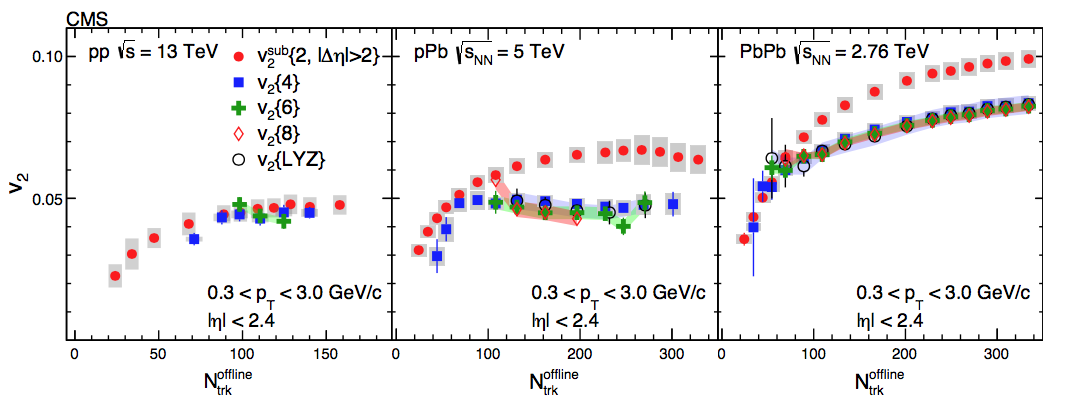
\includegraphics[width=15cm]{FigCap1/v2CumulantsCMS.png}
  \caption{$v_2^{sub} \{2\, |\Delta \eta| > 2\}$, $v_2 \{4\}$, $v_2 \{6\}$, $v_2 \{8\}$ 
  and $v_2 \{LYZ\}$ as a function of the multiplicity, 
  in the interval $0.3 < \pt < 3 \Gevc$ and $|\eta| < 2.4$~\cite{Khachatryan:2016txc} measured by CMS, in pp, p-Pb and Pb-Pb collisions.}
  \label{fig:CumulantsCMS}
\end{figure}
In the left panel of Fig.~\ref{fig:CumulantsCMS}, the $v_2 \{4\}$, $v_2 \{6\}$
measured by CMS in pp collisions at $\sqrt{s} = 13$ TeV are shown as a 
function of the particle multiplicity, in the interval $0.3 < \pt < 3 \; \Gevc$ and 
$|\eta| < 2.4$. In the middle and right panels of the same figure, also the $v_2 \{8\}$ and $v_2 \{ {\rm LYZ} \}$ 
(from Lee-Yang zeros method~\cite{Bhalerao:2003yq}) coefficients are shown, for p-Pb and Pb-Pb collisions
at $\sNN = $ 5 TeV and $\sNN = $ 2.76 TeV respectively.
$v_2 \{8\}$ and $v_2 \{ {\rm LYZ} \}$ are less affected by non-flow correlations, 
thus are expected to give the 
cleanest values of the genuine collective flow.
The values of $v_2 \{4\}$, $v_2 \{6\}$ and of $v_2 \{8\}$ and  $v_2 \{ {\rm LYZ} \}$, where present, are compatible among 
them in each of the three colliding system. This supports the idea 
of a collective behaviour behind the long-range correlations observed in pp 
collisions. In alternative to the classical scenario of position-space
anisotropy that must be transposed into final observed momentum-space anisotropies, other theoretical 
calculations, such as the color glass condensate glasma model~\cite{Schenke:2016ksl}, 
interpret the collective behaviour as due to momentum space-anisotropies that are
already present before the collision via initial interactions of gluons inside the projectile proton or
nucleus. Besides, in Fig.~\ref{fig:CumulantsCMS} the 
$v_2^{sub} \{2$, $|\Delta \eta| > 2\}$, defined from two-particle 
$\Delta \eta$, $\Delta \phi$ correlation after subtraction of jet correlations from low-multiplicity events, 
is also shown. Some hydrodynamical models interpret the similar magnitude 
of $v_2 \{4\}$ and $v_2^{sub} \{2$, $|\Delta \eta| > 2\}$ in pp collisions as the 
consequence of smaller number of initial fluctuating source than in p-Pb and 
Pb-Pb collisions.\\
Recently, ALICE reported about the first observation of strangeness production
 enhancement in high-multiplicity pp collisions~\cite{ALICE:2017jyt}. As 
 anticipated in~\ref{subsec:StrangEnhancSPS}, strangeness enhancement 
 was originally proposed as a signature of the Quark-Gluon Plasma and 
 verified to be even more pronounced for multi-strange baryons. The production 
 of strange hadrons in heavy-ion collisions can be described using a 
 grand-canonical statistical model and does not show a significant dependence 
 on the collision centrality, if one excludes the very peripheral events. For the latter,
  the relative yield of strange particles to pions becomes very similar to what 
  observed in pp and in p-Pb~\cite{Abelev:2013haa,Adam:2015vsf} collisions, and this is understood
  in terms of canonical suppression~\cite{Tounsi:2001ck}. In~\cite{ALICE:2017jyt}, ALICE presented the
   measurement of the production of primary strange ($K^0_S,\; \Lambda,\; \bar{\Lambda}$) 
   and multi-strange ($\Xi^-,\; \Xi^+,\; \Omega^-,\; \Omega^+$) hadrons in pp 
   collisions at $\sqrt{s} = 7$ TeV. Fig.~\ref{fig:StrangenessALICEpp} (left panel) 
   shows the $\pt$-differential yields of 
   $K^0_S,\; \Lambda + \bar{\Lambda},\; \Xi^- + \Xi^+,\; \Omega^- + \Omega^+$ 
   at mid-rapidity, for a selection of classes of events with progressively lower 
   multiplicity, indicated by roman numbers in bracket in the figure. It can be 
   noticed that the $\pt$ spectra become harder as the multiplicity increases, 
   and the hardening becomes stronger with increasing particle mass. This is
    a feature already observed in p-Pb collisions~\cite{Abelev:2013haa} and 
    typically characterizing Pb-Pb collisions, where they are described in terms 
    of relativistic hydrodynamical expansion. A simultaneous fit with the 
    blast-wave model to all $\pt$ spectra in the common highest multiplicity class 
    (I in Fig.~\ref{fig:StrangenessALICEpp} left) and in defined $\pt$ ranges allowed the 
    extraction of the chemical freeze-out temperature $T_{fo} = 163 \pm 10$ 
    MeV and the transverse velocity of the bulk 
    $\langle \beta_{\perp} \rangle = 0.49 \pm 0.02$. The $\pt$ distribution were
     then fitted in their full $\pt$ range using a Tsallis-Lèvy function to obtain the 
     $\pt$-integrated yields. Finally, the right panel of Fig.~\ref{fig:StrangenessALICEpp}
      shows the ratio of $\pt$-integrated hadron yields to the pion yields, as a 
      function of the charged-particle multiplicity, together with the measurements
       in p-Pb ($\sNN = 5.02$ TeV) and Pb-Pb ($\sNN = 2.76$ TeV) collisions. 
       Despite the different energy of the collisions, the ratios show a smooth 
       increase from pp to most central Pb-Pb collisions, with the highest multiplicity 
       points in pp being fully compatible with the magnitude of the enhancement in 
       p-Pb at same multiplicity values or in most peripheral Pb-Pb collisions. At higher multiplicities,
       the ratios in Pb-Pb collisions do not show particular dependence on the collision centrality. This 
       suggests that the mechanism of strangeness enhancement is rather related
        with the characteristics of the final state produced in the collisions, than the
         characteristics of the collision itself. Still, the physical mechanism remains 
         unclear, since the available models fail in reproducing at the same time both
          the ratios in Fig.~\ref{fig:StrangenessALICEpp} and the $\pt$-integrated 
          proton to pion ratios at mid-rapidity~\cite{ALICE:2017jyt}.
\begin{figure}[!ht]
  \centering
  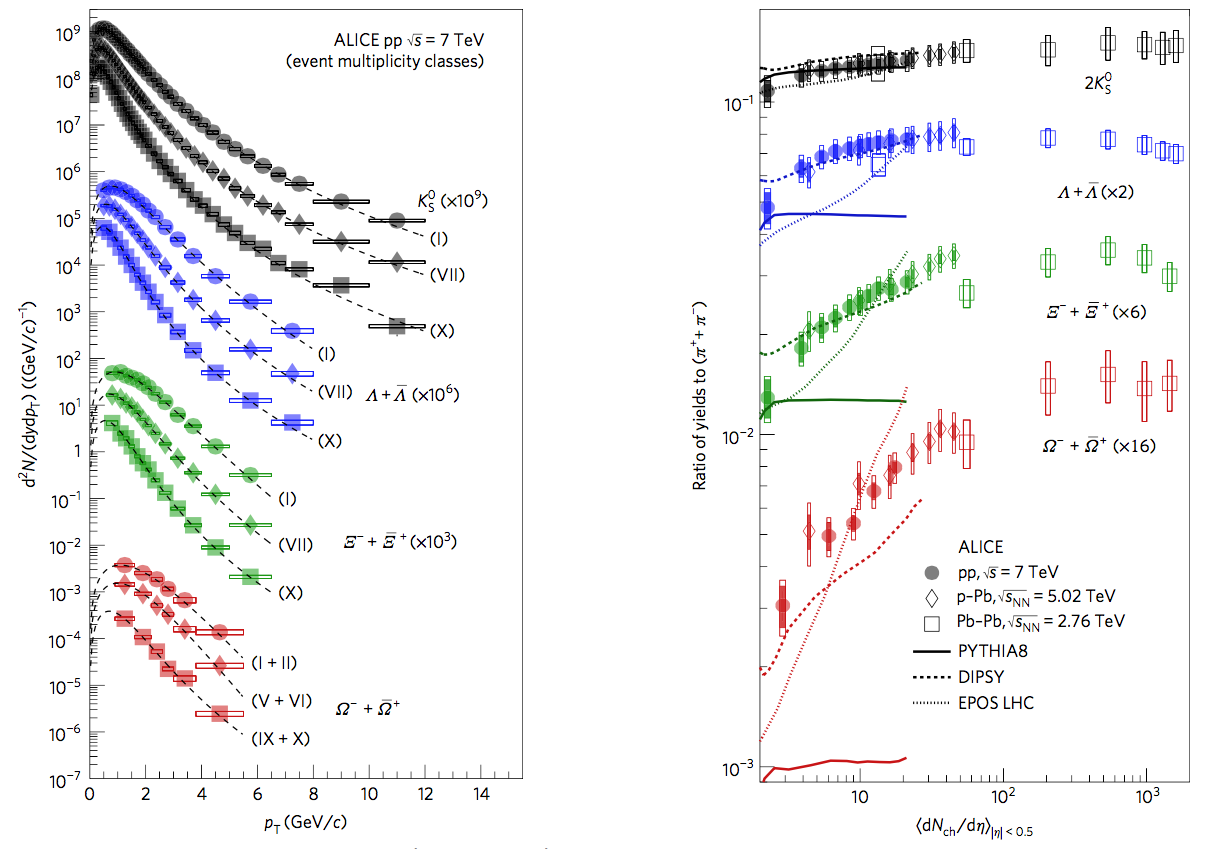
\includegraphics[width=14cm]{FigCap1/StrangenessALICEpp.png}
  \caption{Left: $\pt$-differential yields of $K^0_S,\; \Lambda + \bar{\Lambda}, \Xi^- + \Xi^+,\; \Omega^- + \Omega^+$ at mid-rapidity, for a selection of classes of events with progressively lower multiplicity. The Tsallis-Lèvy fit is shown as dashed line. Right: $\pt$-integrated ratios of $K^0_S,\; \Lambda + \bar{\Lambda},\; \Xi^- + \Xi^+,\; \Omega^- + \Omega^+$ to pion yield ($\pi^- + \pi^+$) as a function of $\langle dN_{ch}/d\eta \rangle$ at mid-rapidity~\cite{ALICE:2017jyt}.}
  \label{fig:StrangenessALICEpp}
\end{figure}














\chapter{Heavy flavours} % Main chapter title
\label{Chapter2} % For referencing the chapter elsewhere, use \ref{Chapter1} 

\section{The importance of being heavy}
\label{sec:introChap2}
Hadrons carrying heavy flavour (charm or beauty quarks) 
constitute a powerful probe to study 
the properties of the Quark-Gluon Plasma created in high-energy 
heavy-ion collisions. Heavy quarks are produced in initial hard parton-scattering processes
of the nucleon-nucleon collisions and on short time scales compared 
to the QGP formation time~\cite{Liu:2012ax},
$\tau_0 \sim 1/Q \sim 0.1-1$ fm/c, where $Q$ is the virtuality of the process. 
The minimum virtuality in the production of $c\overline{c}, b\overline{b}$ pair 
corresponds indeed to $2\, m_{c,b}$
implying a space-time scale of $\sim 0.07$ fm for charm and 
$\sim 0.02$ fm for beauty. Furthermore, in contrast with light quarks and gluons, that can be produced or annihilated 
during QGP evolution, heavy quarks have negligible annihilation 
rate~\cite{BraunMunzinger:2007tn} and secondary "thermal" 
charm production from processes like $gg \rightarrow c\overline{c}$ is 
expected to be negligible in the QGP~\cite{Zhang:2007dm}, 
unless the iniial QGP temperatures occur to be much larger than 
those currently reachable at colliders. Therefore,
heavy quarks preserve their identity when traversing 
the fireball and can be used as a probe
to study the interaction with the medium
 constituents, in particular getting access to the 
transport coefficients of the QGP.\\
There are different ways to experimentally detect hadrons 
containing heavy flavours:
\begin{itemize}
\item full reconstruction of exclusive decay channels, 
like $\DtoKpi$ or $B^0 \rightarrow J/\psi K^0_S$;
\item detection of leptons from heavy-flavour hadron decays, for example 
$D, B \rightarrow e, \mu + X$;
\item selection of semi-inclusive decays, 
for example $J/\psi$ mesons displaced 
from the primary vertex (thus, coming from beauty decay) or $\Lambda_c$ and
$\Xi_c$ reconstruction from $e\, \Lambda$ and $e\, \Xi$ pairs;
\item reconstruction of $c-$ and $b-$jets.
\end{itemize}
\section{Heavy-quark production in pp collisions}
\label{sec:HFpp}
The study of heavy flavours in pp collisions is an 
important benchmark of perturbative QCD calculations. 
The large mass of these quarks acts as a cut off; it prevents 
indeed from divergencies in calculation that arise
from collinear gluon radiation and that are suppressed 
in case of massive quarks due to the
so-called dead-cone effect~\cite{Dokshitzer:1991fd}. 
For this reason, perturbative calculations are applicable down to low $\pt$ 
as well as the computation of the total cross-section. 
The two processes responsible for heavy-quark production 
at the leading order in perturbative theory are 
$q \overline{q} \rightarrow Q \overline{Q}$ and $gg \rightarrow Q \overline{Q}$, 
whose corresponding diagrams are
shown in Fig.~\ref{fig:LOdiagrams}. The relative production 
rates for heavy quarks of mass 
$m_1$ and $m_2$ behave, at high energy, as~\cite{Mangano:1997ri}:
\begin{equation}
\begin{aligned}
\frac{\sigma (gg \rightarrow Q_1 \overline{Q}_1)}{\sigma (gg \rightarrow Q_2 \overline{Q}_2)} & \rightarrow 1 - \frac{{\rm log}(m_1^2/m_2^2)}{{\rm log}(s/m_2^2)}, \\
\frac{\sigma (q \overline{q} \rightarrow Q_1 \overline{Q}_1)}{\sigma (q \overline{q} \rightarrow Q_2 \overline{Q}_2)} & \rightarrow 1 - \mathcal{O} (m_1^4/s^2),
\end{aligned}
\end{equation}
hence, at large center-of-mass energy $s$, the 
$q \overline{q} \rightarrow Q \overline{Q}$ process
vanishes more quickly. In the left panel of Fig.~\ref{fig:HQxsecPPcoll}
 the inclusive production cross-section in pp collisions,
as a function of center-of-mass energy, for charm, bottom, 
top quark pairs is shown~\cite{Mangano:1997ri}.
\begin{figure}[!ht]
  \centering
  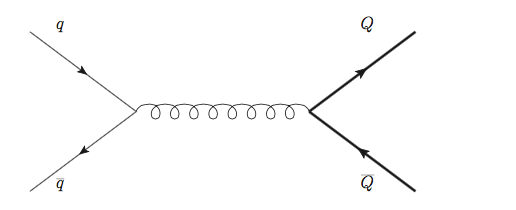
\includegraphics[width=8cm]{FigCap2/Feymann1.png}
  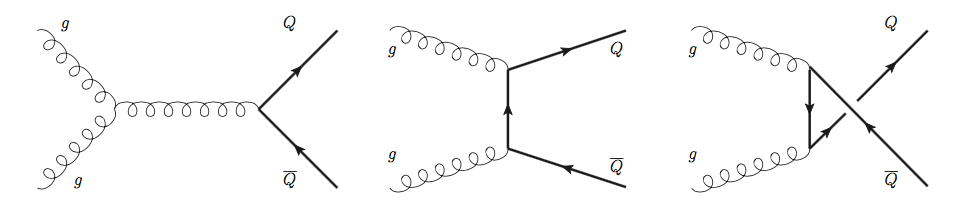
\includegraphics[width=15cm]{FigCap2/Feymann2.png}
  \caption{Leading-order diagrams for heavy-quark pair production.}
  \label{fig:LOdiagrams}
\end{figure}
Analytic calculations that provide a description for inclusive 
heavy-hadron production or their decay products
in pp collisions utilising the collinear factorisation approach 
are FONLL~\cite{Cacciari:1998it,Cacciari:2001td} 
and GM-VFNS~\cite{Kniehl:2004fy}. 
FONLL is a Fixed-Order calculation with Next-to-Leading-Logarithms 
resummation and provides calculations in the full kinematic range 
($\pt \ll m_Q, \pt \sim m_Q, \pt \gg m_Q$),
giving description of bottom and charm production at Tevatron, RHIC and LHC. 
GM-VFNS was originally performed in the massless limit 
and subsequently improved with finite mass terms.
Within both approaches, the single inclusive distribution of a 
heavy-flavour hadron $H_q$ is obtained as a convolution of a
perturbative cross section $d\sigma$ at the partonic level with 
parton distribution functions $f(x, Q^2)$ and non-perturbative 
fragmentation function $D^{NP}_{q->H_q}$.
Possibly a decay function $g^{weak}_{H_q \rightarrow l}$ 
describing, for instance, the hadron weak decay into a lepton can be included:
\begin{equation}
d\sigma_l = f(x, Q^2) \otimes d\sigma_{q} \otimes D^{NP}_{q->H_q} \otimes g^{weak}_{H_q \rightarrow l}.
\end{equation}
The functional form of the non-perturbative fragmentation 
function (FF) $D^{NP}_{q->H_q}$ 
is generally chosen as result of fit on $e^+e^-$ data for 
heavy-hadron production. For example, FONLL uses
a Kartvelishvili et al.~distribution~\cite{Kartvelishvili:1977pi} 
for the FF of bottom quarks:
\begin{equation}
D^{NP}_{b->H_b}= (\alpha +1 )(\alpha +2)z^{\alpha} (1-z),
\end{equation}
where the fragmentation parameter $\alpha$ was chosen as a 
result of the fit on the LEP data concerning production
of a mixture of $b$-hadrons~\cite{Cacciari:2005uk,Heister:2001jg,Abbiendi:2002vt}, 
since no data are available for individual hadrons like $B^0$ or $B^+$.
\begin{figure}[!ht]
  \centering
  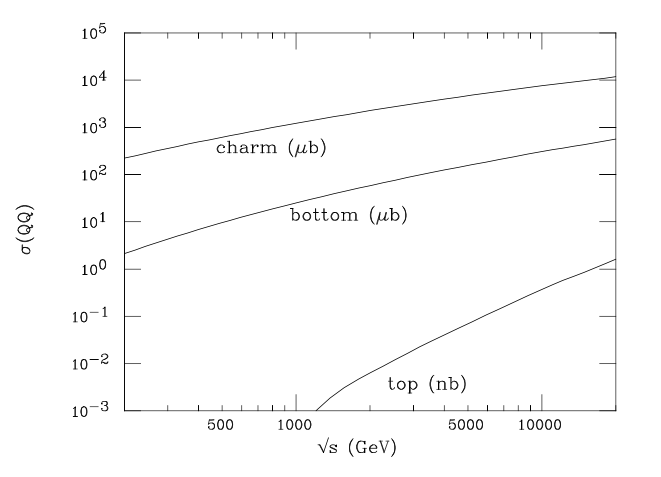
\includegraphics[width=7.6cm]{FigCap2/HQxsecPPcoll.png}
      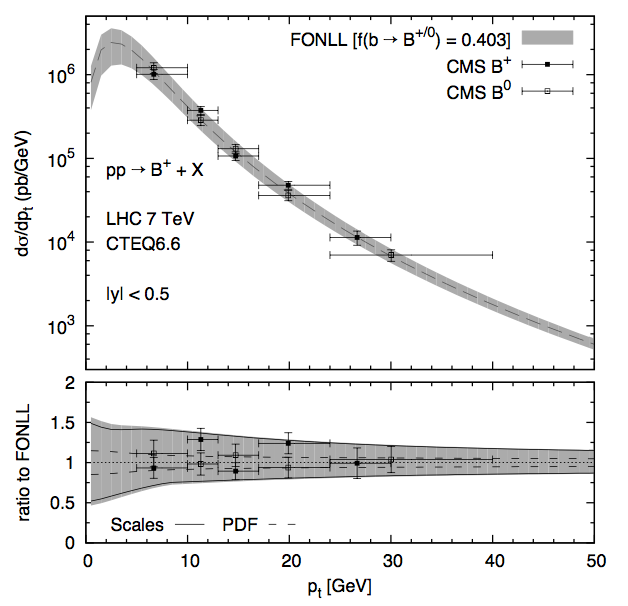
\includegraphics[width=6.4cm]{FigCap2/FONLLBmeson.png}
  \caption{Left: total production cross-sections for charm, bottom and top quark pairs, in pp collisions as a function of the center-of-mass energy~\cite{Mangano:1997ri}. Right: FONLL calculation and systematics band~\cite{Cacciari:2012ny} for beauty-hadron production, rescaled to the $|y| <$ 0.5 region, and comparison with CMS data~\cite{Khachatryan:2011mk,Chatrchyan:2011pw}.}
  \label{fig:HQxsecPPcoll}
\end{figure}
For charm quarks, experimental data for individual D-meson species exist.
Since from the theoretical point of view some differencies are 
expected in the quark fragmentation into 
pseudo-scalar ($\Dzero, \Dplus$) and vector ($\Dstar$) mesons, 
one needs to define two different FF. The functional forms used for
the FF of charm quarks in FONLL are taken from~\cite{Cacciari:2003zu}
and have one single non-perturbative parameter
common to the pseudo-scalar and vector FF. This parameter is adjusted on
ALEPH data~\cite{Barate:1999bg} for $\Dstar$ production.
Fig.~\ref{fig:HQxsecPPcoll} (right) shows the CMS measurement 
of $\pt$-differential cross-section for $B^+$ and $B^0$ mesons
as a function of $\pt$ in the rapidity interval $|y| < 0.5$ in pp collision 
at $\sqrt{s} = 7$ TeV~\cite{Khachatryan:2011mk,Chatrchyan:2011pw}, 
compared to FONLL predictions.
The FONLL uncertainty band is obtained from variations of 
renormalisation scale $\mu$ and common factorisation
scale $\mu_f$ as well as of the heavy-quark mass.
Similar comparison, but for charmed hadrons, is shown in Fig.~\ref{fig:CharmXsec} 
for $\Dzero$-meson production
in pp collision at $\sqrt{s} = 7$ TeV measured by 
ALICE~\cite{Acharya:2017jgo}, as a function of $\pt$. FONLL 
predictions are displayed in the left panel and GM-VFNS in the right one. 
Calculations are in agreement with bottom and charm production 
at the LHC, within their
uncertainties. FONLL central values tend to underestimate charm production, 
that systematically lays on the upper edge of FONLL uncertainty band, 
whereas GM-VFNS tends to slightly overestimate the production 
at high $\pt$ but agrees very well at intermediate-low $\pt$. \\



In contrast to FONLL and GM-VFNS, that are based on NLO 
pQCD calculations and are limited to inclusive production
of heavy quarks and mesons, general-purpose Monte Carlo 
generators, such as PYTHIA~\cite{Sjostrand:2006za}, provide a more complete description 
of the final state, including decay kinematics. They simulate the 
final states of high-energy collisions in full detail, including hard and 
soft interactions, parton distributions, initial- and final-state parton 
showers, multiparton interactions, fragmentation and decay. They contain a large 
list of hard Standard Model and Beyond Standard Model processes, 
which are interfaced with parton emission, different models of hadronisation and particle decays. 
The processes are treated at leading order (LO). The higher order 
calculations are included only in an
approximate approach. However, the next-to-leading order (NLO) 
is needed to compare results with experimental data.
PYTHIA generator, for example, contains 
theoretical perturbative QCD calculations that are exact only
at leading order, where only the pair creation processes 
$q\overline{q} \rightarrow Q\overline{Q}$ and $gg \rightarrow Q\overline{Q}$
are included. Higher-order contributions at the NLO to account 
for flavour excitation processes like $qQ \rightarrow qQ$, $gQ \rightarrow gQ$
and the gluon splitting $g \rightarrow Q\overline{Q}$ are also accounted. 
The cross-section of these processes 
diverges as the transverse momentum of the outgoing quarks of the 
hard interaction ($\pt^{hard}$) goes to zero. 
The divergences can be controlled by a lower cut 
on the value of  $\pt^{hard}$, that has a large influence in the 
heavy-flavour production 
in the low-$\pt$ region, which is of the prime interest for ALICE. 
To compare PYTHIA to data, $\pt^{hard}$ and
other PYTHIA parameters must be tuned to reproduce as well 
as possible NLO predictions.
The first generator of heavy-quark production that did the effort of matching NLO calculations 
with LO calculations was MC@NLO~\cite{Frixione:2002ik}.
It proposed a first solution to the double counting of NLO events, 
by subtracting the approximated 
NLO cross section (which were implemented in the general generators)
 from the exact NLO cross section.
The NLO calculations for the hard processes in heavy-flavour production are obtained within the 
POWHEG~\cite{Frixione:2007nw} (Positive Weight Hardest Emission Generator) method. 

\begin{figure}[!ht]
  \centering
  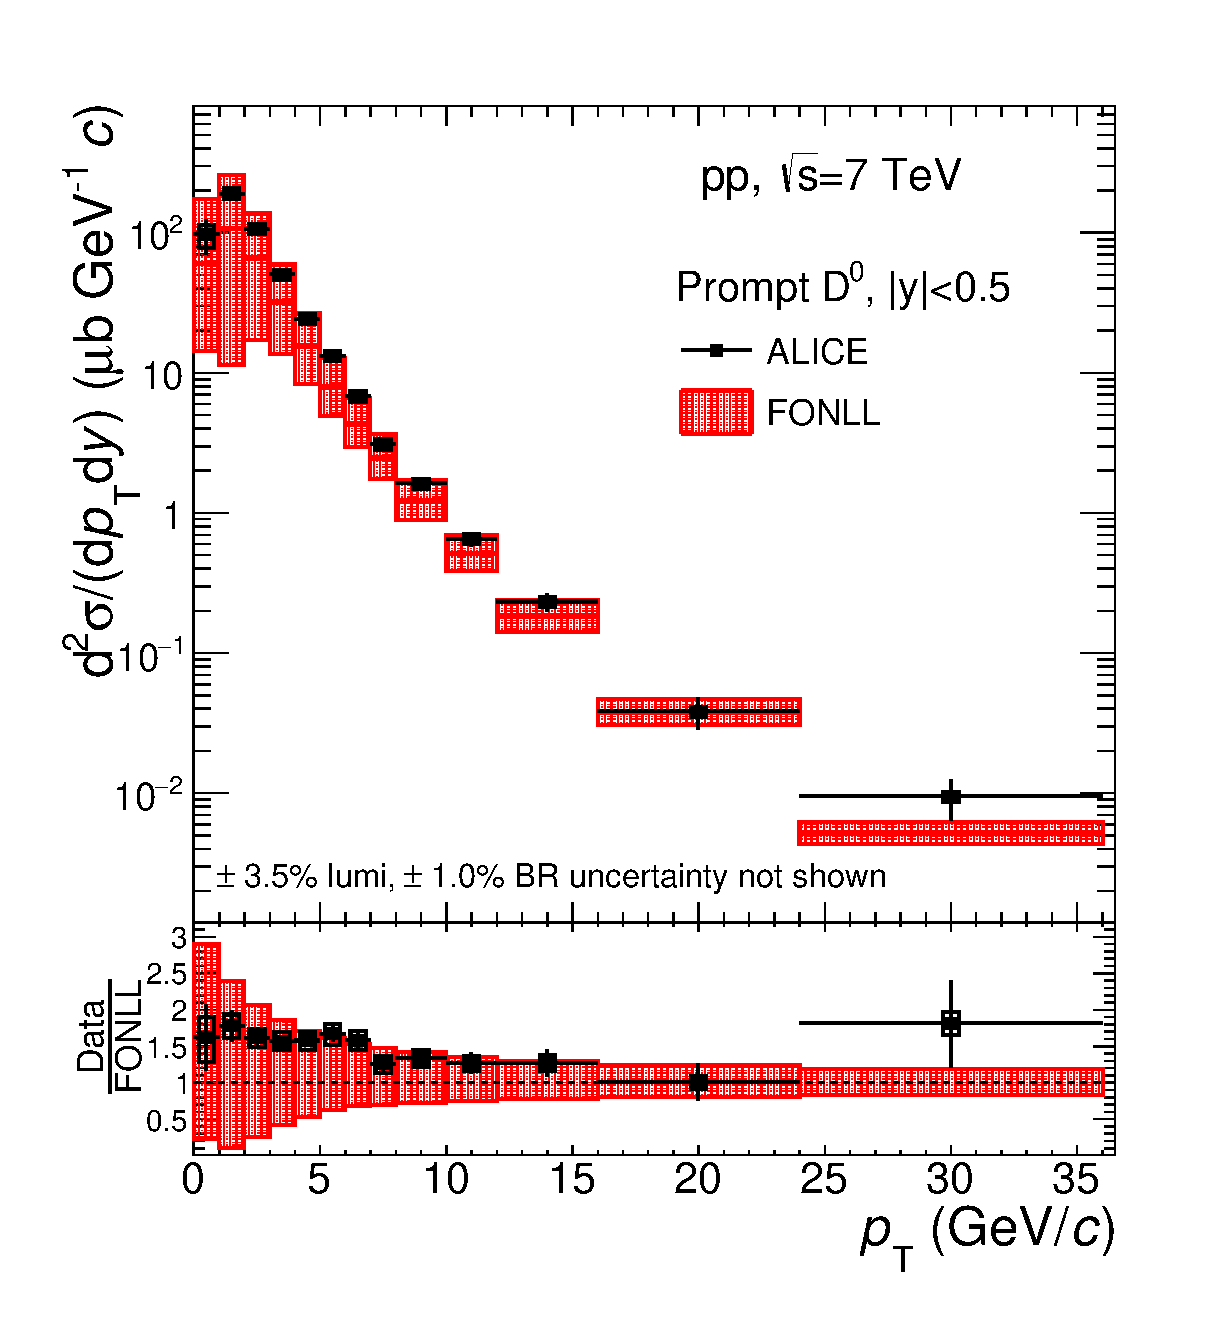
\includegraphics[width=7cm]{FigCap2/DzeroppCrossSecVsFONLLAndRatio.eps}
  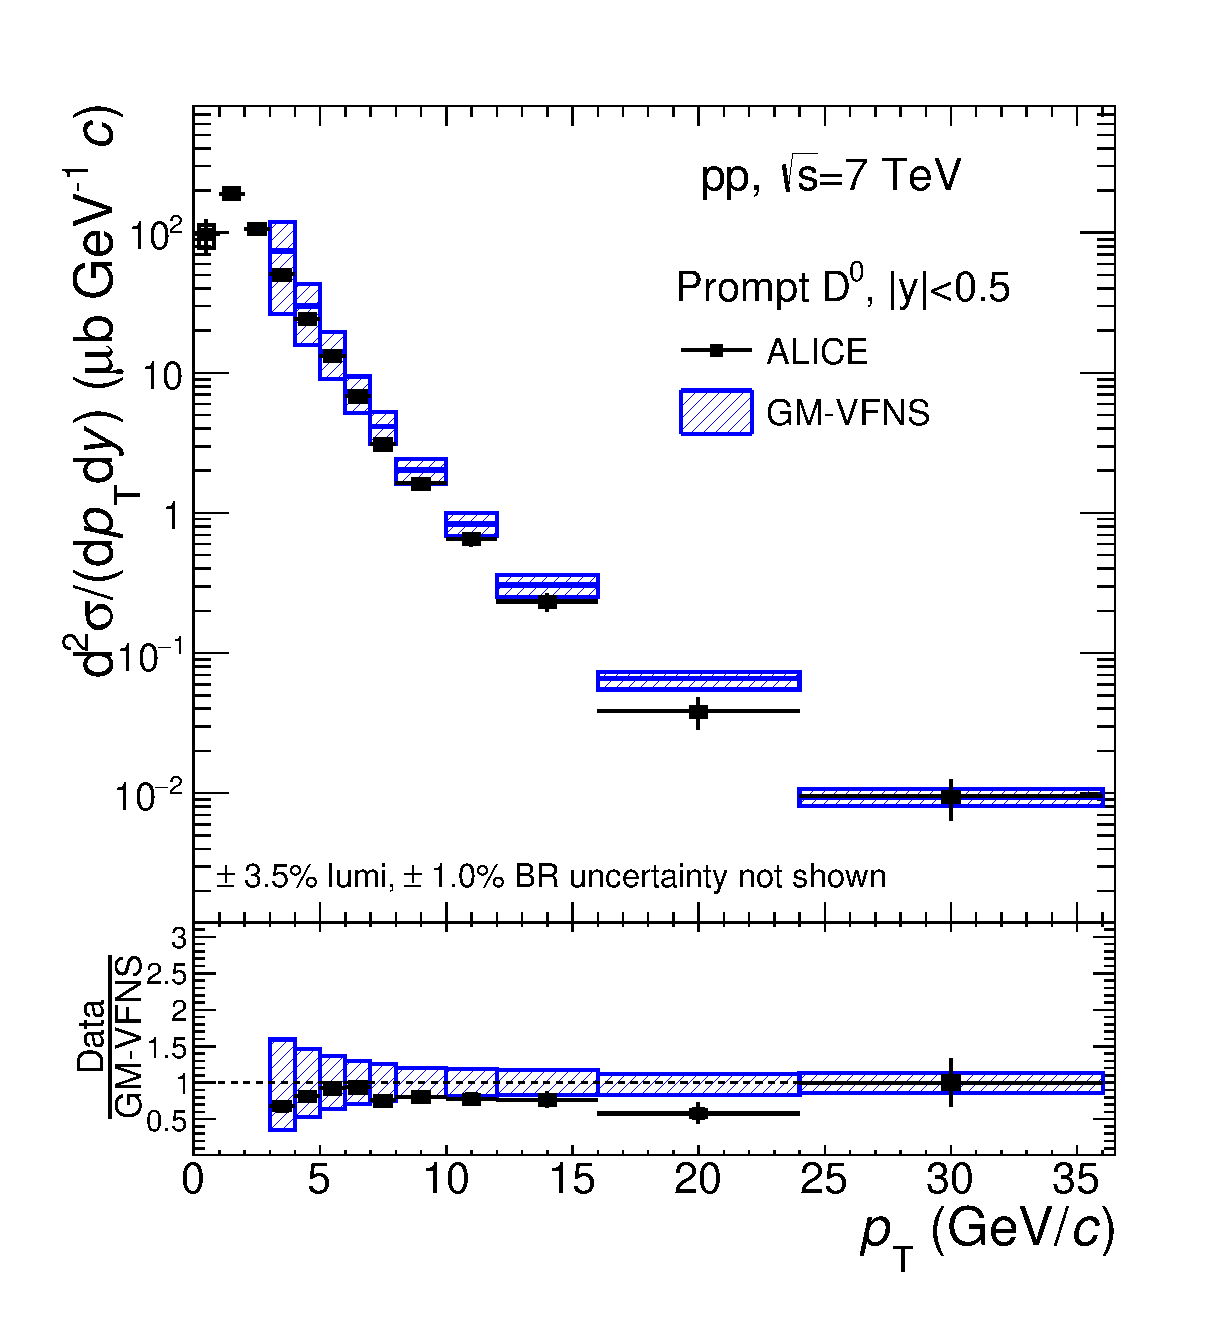
\includegraphics[width=7cm]{FigCap2/DzeroppCrossSecVsGMVFNSAndRatio.eps}
  \caption{$\pt$-differential production cross section of prompt $\Dzero$ mesons with $|y| < $ 0.5 in the interval $0 < \pt < 36 ~\Gevc$, in pp collisions at $\sqrt{s} = 7$ TeV~\cite{Acharya:2017jgo}. The cross section is compared to pQCD calculations: FONLL~\cite{Cacciari:1998it,Cacciari:2001td} (left panel) and GM-VFNS~\cite{Kniehl:2004fy} (right panel).}
  \label{fig:CharmXsec}
\end{figure}

\section{Heavy quarks in p-A collisions}
\label{sec:HFpA}
\subsection{Cold nuclear matter effects}
\label{sec:CNM}
The importance of studying heavy-flavour production in p-A collisions relies on the possibility to
characterise a class of phenomena that are expected to break the binary scaling in 
nucleus-nucleus collisions but are not a consequence of the presence of a 
deconfined plasma. Such effects can in fact be present both in p-A and in A-A collisions and
their origin is mainly related to modification of the PDFs for nucleons bound in nuclei and
multiple soft scatterings of the partons in the nuclei prior to the
hard interaction energy loss in cold nuclear matter. 
They are usually called Cold Nuclear Matter (CNM) effects and
can affect the partons that undergo the hard 
scattering process (initial-state effects) as well as
the produced heavy quarks and hadrons (final-state effects).
Furthermore, recent interest in p-A collisions
is focused on revealing possible effects that could indicate the 
formation of a QGP droplet in small collision systems~\cite{Beraudo:2015wsd,Bozek:2014era,Bzdak:2013zma}.

\subsection{Nuclear Parton Distribution Functions}
\label{sec:nPDFs}
One can quantify the nuclear modification for the parton distribution function via the ratio:
\begin{equation}
\label{eq:RA}
R_i^A(x,Q^2) = f_{i/A}(x,Q^2) / f_{i/p}(x,Q^2)
\end{equation}
\begin{figure}[!ht]
  \centering
  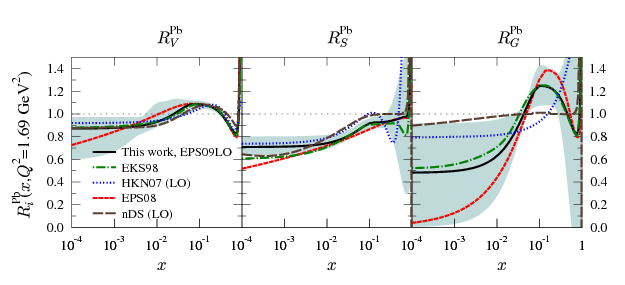
\includegraphics[width=15cm]{FigCap1/PartonNMF.png}
  \caption{The nuclear modification factor (Eq.~\ref{eq:RA}) in a Pb nucleus $R_i^A(x,Q^2)$ for three different flavours as given by the available nPDF parameterizations at LO~\cite{Eskola:2009uj}.}
  \label{fig:nPDF}
\end{figure}
where $f_{i/A}(x,Q^2)$ and $f_{i/p}(x,Q^2)$ are the parton distribution functions in the 
nucleus and in the proton respectively, and the variable $x$ represents the fraction of 
the nucleon momentum carried by a parton. Fig.~\ref{fig:nPDF} 
shows the ratios $R_i^A(x,Q^2)$ for the valence quarks, sea quarks and 
gluons inside a Pb nucleus as obtained from LO global DGLAP 
calculations with EKS98~\cite{Eskola:1998df,Eskola:1998iy}, 
EKPS~\cite{Eskola:2007my},
nDS~\cite{Eskola:2008ca}, HKN07~\cite{Hirai:2007sx} and EPS09LO~\cite{Eskola:2009uj}
parameterisations of the nuclear PDFs which are tuned on measurements
of DIS, Drell-Yan and hadron and dijet production in p-A collisions. 
In general, four different regions are visible in the trend of $R_i^A(x,Q^2)$ versus $x$,
which correspond to four $x$-regimes in which different 
effects influence the PDFs of bound nucleons:
\begin{itemize}
\item {\bf Fermi motion:} this effect is due to the 
thermal momentum that nucleons have inside the nucleus. 
Thus the structure function $F^A_2(x)$ of the bound nucleons
is the convolution of the structure function of the free nucleon 
$F^N_2(x/z)$ (where $z$ is the momentum fraction
of the nucleons times the atomic number of the nucleus) 
with the momentum distribution
of nucleons $f_N(z)$ inside the nucleus: 
$F^A_2(x) = \int_x^A dz f_N(z) F_2^N(x/z)$.
This is the dominant effect for $x > 0.7$.
\item {\bf EMC effect:} first observed in 1982 by EMC collaboration~\cite{Aubert:1983xm},
this effect appears as $R_i^A(x,Q^2)<1$, especially affecting the region 
of valence quarks $0.2 < x < 1$. Fig.~\ref{fig:EMC} left shows the ratio of the structure functions 
of iron $F^{iron}_2(x)$ and deuterium $F^D_2(x)$, that one would expect to be at 1 (except for 
some corrections at high $x$ from Fermi motion). From further
experimental investigations, it was clear that the effect is almost independent from the 
squared momentum transfer, it increases with nuclear mass 
number A and scales approximately with the average nuclear density. 
Many phenomenological models tried to explain such behaviour. 
In the $Q^2$-rescaling models, 
quarks in nuclei move in a larger confinement volume and, 
because of the uncertainty principle, 
they carry less momentum than quarks in free nucleons. 
Some models proposed that 
quarks in nuclei move in quark bags with $n$ quarks, 
other proposed an enhancement 
of pion-cloud effects and a nuclear pionic field, 
but no models so far are universally accepted. 
\iffalse
 In 2009 other pieces of information were added with the
discovery of a strong correlation between the slope of the ratio $R_i^A(x,Q^2)$ in 
the region of EMC effect and the magnitude of the scaling plateau 
at $x > 1$ (see Fig.~\ref{fig:EMC}, right panel)~\cite{Seely:2009gt}.
\fi
\item {\bf Nuclear shadowing and anti-shadowing:} a second depletion region
is observed in the ratio of parton distribution functions $f_{i/A}(x,Q^2) / f_{i/p}(x,Q^2)$ 
at very low $x<0.01$ (typical region of sea quarks). This is commonly denoted 
by shadowing region and is accompanied by
an anti-shadowing region at $0.01 < x < 0.2$ in which the ratio $R_i^A(x,Q^2)$
is above unity.~Different models were
proposed to explain the nuclear shadowing. Some models are based on virtual 
photon fluctuations into vector meson states (GVMD); others
invoke superposition ad fusion of partons of different nucleons at very low $x$, that should deplete the 
region, thus favouring the population of the anti-shadowing region.

\end{itemize}


\begin{figure}[!ht]
  \centering
  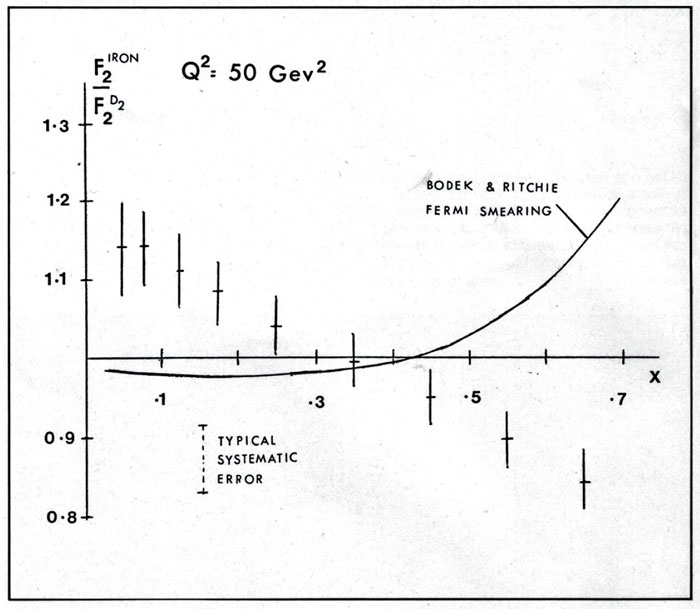
\includegraphics[width=7cm]{FigCap2/EMC.jpg}
%  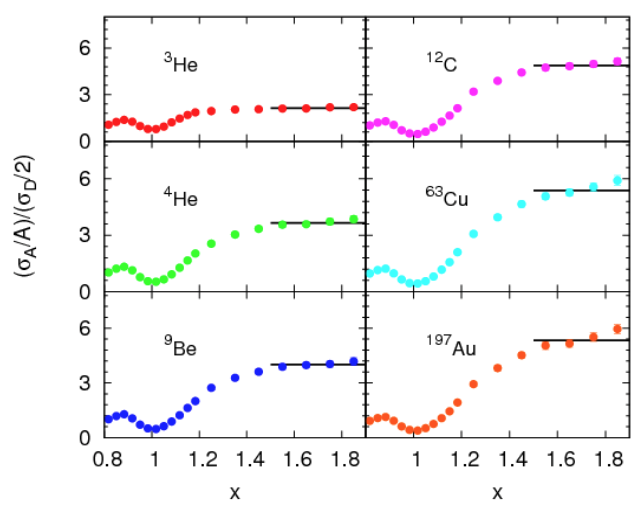
\includegraphics[width=7.5cm]{FigCap2/EMC2.png}
  \caption{Ratio of iron $F^{iron}_2(x)$ and deuterium $F^D_2(x)$ structure function as a function of Bjorken-$x$~\cite{Aubert:1983xm}.% Right: ratio of nucleus $F^{A}_2(x)$ and deuterium $F^D_2(x)$ for different nuclei as a function of Bjorken-$x$~\cite{Seely:2009gt}.
  }
  \label{fig:EMC}
\end{figure}



An other CNM effect is the so-called Cronin Effect~\cite{Cronin:1974zm}, 
discovered in the '70s at FermiLab. It consists in an observed 
enhancement in the nuclear modification factor for $\pt$ 
values between 2 and 5 $\Gevc$. This is commonly understood as due to 
the fact that, in p-A collisions, the 
partons of the projectile nucleon undergo several elastic 
scatterings with the partons of the target nucleus before the hard scattering process 
occurs. The multiple scatterings give the parton an extra 
momentum component in the transverse plane ($k_{\rm T}$ broadening), 
which causes a broadening of the $\pt$ spectra of the heavy 
quarks produced in the hard scattering processes,  
resulting in an enhancement of the nuclear modification factor at 
low and intermediate $\pt$. Going towards 
larger values of transverse momentum, the extra-$k_{\rm T}$ 
from the elastic collisions becomes negligible and the nuclear 
modification factor gets close to unity.\\
%The x regime relevant for charm production at the LHC ($\sim 10^{-4}$ ) is about 2 orders of magnitude lower than at RHIC and 3 orders of magnitude lower than at the SPS [43]. In this region with low x-values, modifications of the nuclear PDFs are mainly related to the shadowing effect.
\begin{figure}[!ht]
  \centering
  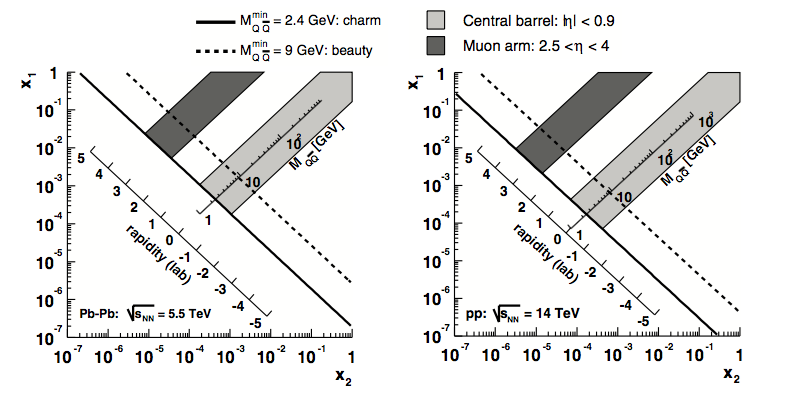
\includegraphics[width=15cm]{FigCap2/xBjork.png}
  \caption{ALICE acceptance in the ($x_1, x_2$) plane for heavy flavours in Pb-Pb at $\sNN = 5$ TeV on the left panel and pp collisions at $\sqrt{s} = 14$ TeV on the right~\cite{Alessandro:2006yt}. }
  \label{fig:xBjork}
\end{figure}



Let's turn now to understand which are the ranges of Bjorken $x$
at play when producing $c\overline{c}$ and $b\overline{b}$ pairs at the LHC. 
The probed $x$ value depends on the center-of-mass energy
of the collision, on the invariant mass $M_{Q\overline{Q}}$ of the 
$Q\overline{Q}$ pair produced in the hard scattering
and on its rapidity $y_{Q\overline{Q}}$. Under the hypothesis 
that the transverse momentum of the parton 
in the nucleon is negligible, the four-momenta of the two 
incoming gluons are $(x_1,0,0,x_1)\cdot(Z_1/A_1)\sqrt{s_{\rm pp}}/2$
and $(x_2,0,0,-x_2)\cdot(Z_2/A_2)\sqrt{s_{\rm pp}}/2$, where 
$x_1$ and $x_2$ are the momentum fractions 
carried by the gluons, and $\sqrt{s_{\rm pp}}$ is the c.m.s. energy for pp collisions,
that differs from the c.m.s $\sNN$ energy of colliding nuclei by the factor $Z/A$. 
The square of the invariant mass of the produced $Q\overline{Q}$ pair is given by:
\begin{equation}
\label{eq:Mqq}
M_{Q\overline{Q}}^2 =  x_1 x_2 s_{\rm NN} = x_1 \frac{Z_1}{A_1} x_2 \frac{Z_2}{A_2} s_{\rm pp},
\end{equation}
and the rapidity in the laboratory is:
\begin{equation}
\label{eq:yqq}
y_{Q\overline{Q}} = \frac{1}{2} {\rm ln} {\Big [ } \frac{E +p_z}{E-p_z}  {\Big ] }= \frac{1}{2} {\rm ln} {\Big [ } \frac{x_1}{x_2} \cdot \frac{Z_1 A_2}{Z_2 A_1} {\Big ] }.    
\end{equation}
From Eq.~\ref{eq:Mqq} and~\ref{eq:yqq} and for a symmetric colliding system $(A_1 = A_2, Z_1 = Z_2)$
one obtains:
\begin{equation}
\label{eq:x1x2}
x_1 = \frac{M_{Q\overline{Q}}}{\sqrt{s_{\rm NN}}} {\rm exp} (+y_{Q\overline{Q}} ), \; \; \; \; \; \;
x_2 = \frac{M_{Q\overline{Q}}}{\sqrt{s_{\rm NN}}} {\rm exp} (-y_{Q\overline{Q}} ). 
\end{equation}\\




Because of its lower mass, charm allows to probe lower $x$ values than beauty. 
The $x$ regime relevant for charm production at the LHC ($\approx 10^{-4}$) is about 
2 orders of magnitude lower than at RHIC and 3 orders of magnitude lower than at the SPS.
Measurements of charm and beauty particles in the forward (or backward) rapidity region ($|y| \sim 4 $) 
gives access to $x$ regimes about 2 orders of magnitude lower, down to $x \approx 10^{-6}$.
Fig.~\ref{fig:xBjork}~\cite{Alessandro:2006yt} shows the ($x_1, x_2$) 
plane for charm and bottom production at the LHC
covered by the ALICE acceptance, for Pb-Pb
collisions at $\sNN = 5$ TeV on the left panel and pp collisions 
at $\sqrt{s} = 14$ TeV on the right.
The shadowed regions correspond to the rapidity region covered 
by the ALICE central barrel ($|\eta| < 0.9$) and by the 
muon arm ($-4 < \eta < -2.5$).
The points with equal invariant mass ($c\overline{c}$ and $b\overline{b}$ pairs) lie on hyperbolae (straight lines in the log-log scale).\\


\subsection{Experimental results in p-A collisions}
\label{sec:HFresultspA}
The nuclear modification of the PDFs can significantly affect final hadrons yields,
especially at low $\pt$ due to shadowing, which is the most relevant effect at LHC energies.
One can define the nuclear modification factor for p-Pb collisions as:
\begin{equation}
R_{\rm pPb} = \frac{1}{A}\frac{d^2\sigma_{pPb}^{\rm prompt D}/d\pt dy}{d^2\sigma_{pp}^{\rm prompt D}/d\pt dy},
\end{equation}
where A is the Pb mass number $A = 208$. \\
\begin{figure}[!ht]
  \centering
  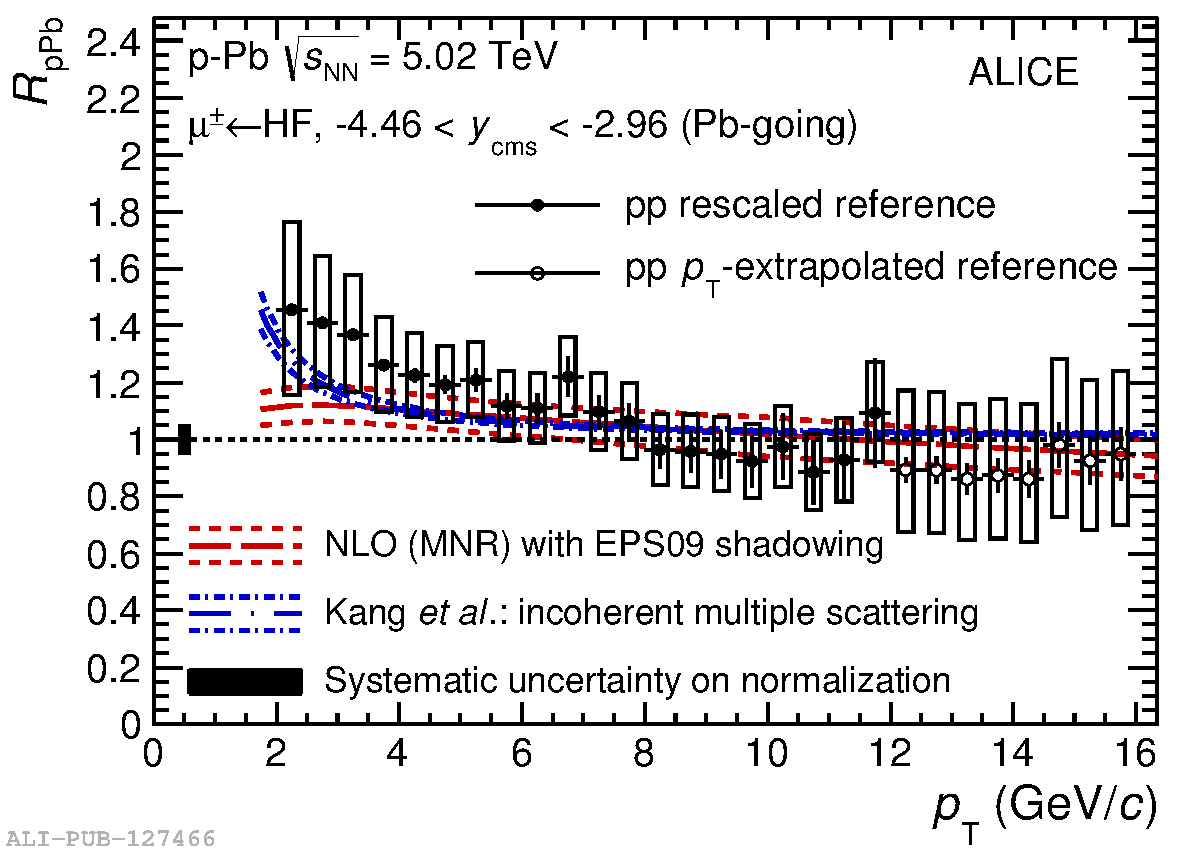
\includegraphics[width=7cm]{FigCap2/2017-Feb-05-Fig2b.pdf}
  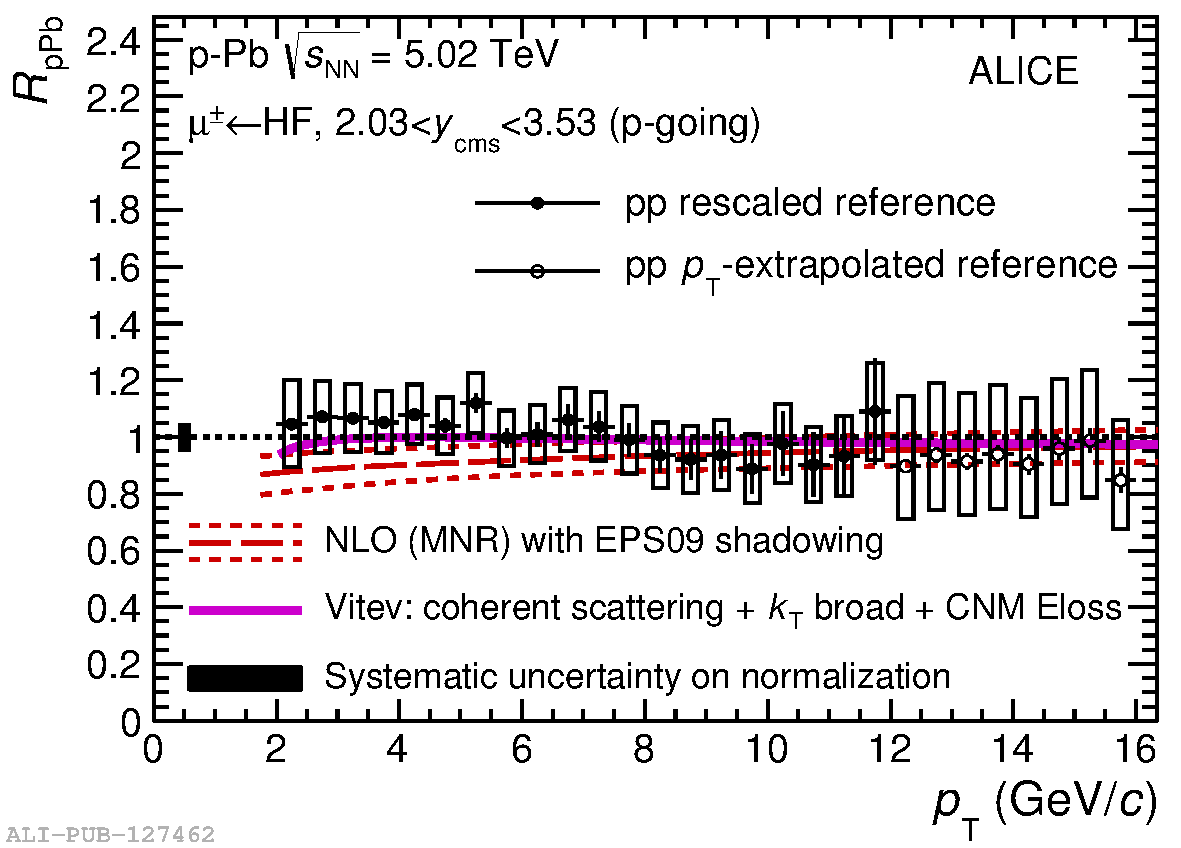
\includegraphics[width=7cm]{FigCap2/2017-Feb-05-Fig2a.pdf}
  \caption{Nuclear modification factor of muons from heavy-flavour hadron decays as a function of $\pt$ for p-Pb collisions at $\sNN = 5.02$ TeV at backward rapidity ($4.46 < y_{\rm cms} < 2.96$, left) and forward rapidity ($2.03 < y_{\rm cms} < 3.53$, right)~\cite{Acharya:2017hdv} compared to model predictions~\cite{Kang:2014hha,Mangano:1991jk}. }
  \label{fig:muons}
\end{figure}
\begin{figure}[!ht]
  \centering
    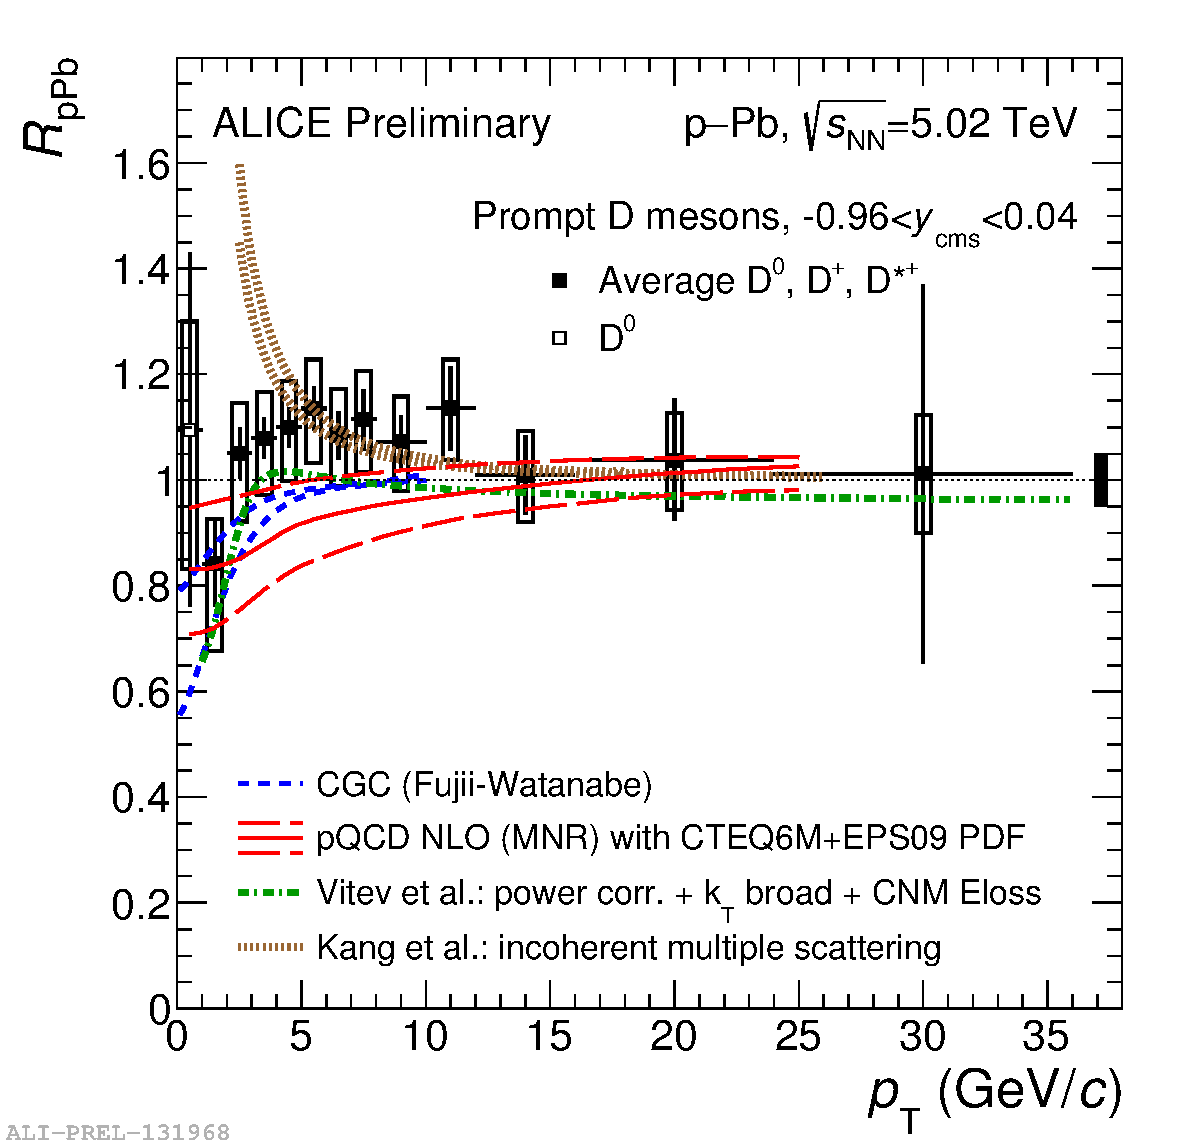
\includegraphics[width=7cm]{FigCap2/2017-Jul-05-pPbWithModelsCNM.pdf}
    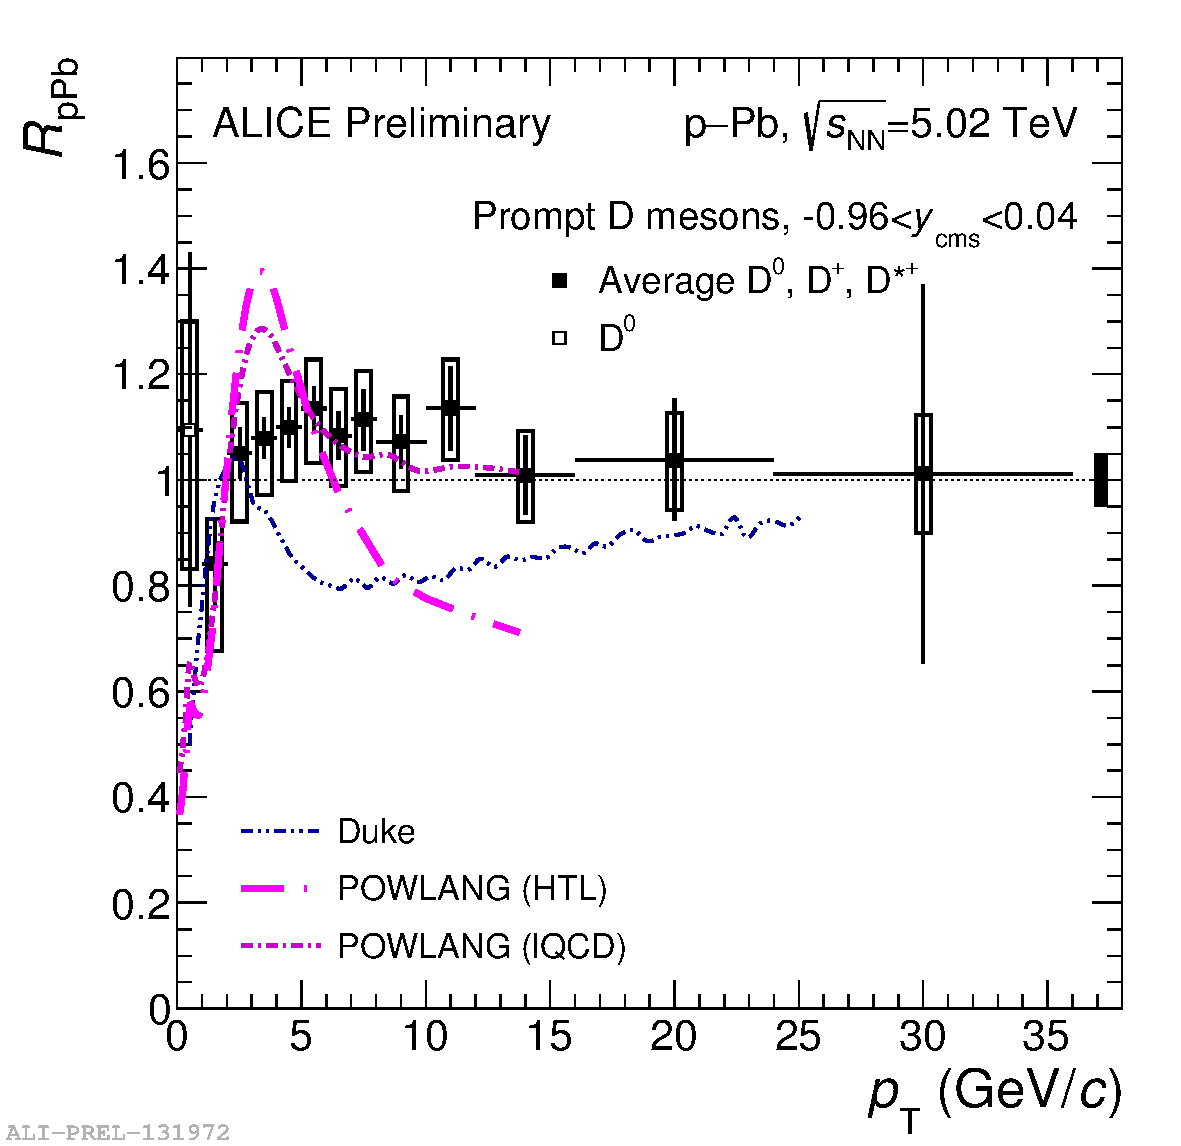
\includegraphics[width=7cm]{FigCap2/pPbWithModelsMedium.pdf}
  \caption{Left: nuclear modification factor $R_{\rm pPb}$ of prompt D mesons in p-Pb collisions at $\sNN = 5.02$ TeV. Data are compared with results of theoretical calculations including only CNM effects~\cite{Fujii:2017rqa,Cacciari:2012ny,Eskola:2016oht,Sharma:2009hn,Kang:2014hha}. Right: the results of the Duke~\cite{Xu:2015iha} and POWLANG~\cite{Beraudo:2015wsd} transport models are compared with the measured D-meson $\RpPb$.}
  \label{fig:RpA}
\end{figure}


ALICE measured the $\pt$-differential nuclear modification factor 
$R_{\rm pPb}$ of muons from heavy-flavour hadron decays in p-Pb collisions at $\sNN = 5.02$ TeV
at forward and backward rapidity~\cite{Acharya:2017hdv} (Fig.~\ref{fig:muons}).
While at forward rapidity muon $R_{\rm pPb}$ is compatible 
with unity in the full $\pt$ range ($2 <\pt < 16 \, \Gevc$) in which the 
measurement was carried out, 
at backward rapidity, it is larger than unity at low $\pt$ with a maximum 
deviation of $R_{\rm pPb}=1$ of 2.2$\sigma$ of the combined statistical and 
systematic uncertainties in the interval $2.5 < \pt < 3.5 \;\Gevc$. 
At higher $\pt$, it is compatible with unity. The results indicate
that CNM effects are small and that the strong suppression of the
yields of muons from heavy-flavour hadron decays observed in the
10\% most central Pb-Pb collisions~\cite{Abelev:2012qh} should result from final-state
effects, i.e. the heavy-quark in-medium energy loss. 
ALICE also measured the $R_{\rm pPb}$ of prompt 
D mesons in p-Pb collisions at $\sNN = 5.02$ TeV
as a function of $\pt$ and the results are shown in 
Fig.~\ref{fig:RpA} (left panel)~\cite{ALICEPAS2017008}. 
Data are compared to theoretical models that include CNM effects: 
a calculation based on the Color Glass Condensate
formalism~\cite{Fujii:2013yja,Fujii:2017rqa}, a FONLL 
calculation~\cite{Cacciari:2012ny} with CTEQ6M PDFs~\cite{Pumplin:2002vw} 
and EPPS16 NLO nuclear modification~\cite{Eskola:2016oht}, 
a LO pQCD calculation with intrinsic $k_{\rm T}$ broadening, 
nuclear shadowing and energy loss of the charm quarks 
in cold nuclear matter (Vitev et al.)~\cite{Sharma:2009hn}, 
and a higher-twist calculation based on incoherent multiple 
scatterings (Kang et al.)~\cite{Kang:2014hha}. 
The three former calculations describe the data within 
uncertainties in the entire $\pt$ range, although for the CGC 
calculation the compatibility with the data 
in 3-12 $\Gevc$ is at the limit of the uncertainties of the data 
and of the calculations. The calculation by Kang et al., which has 
a different trend with respect to the others, is disfavoured by the 
data for $\pt<3$--$4~\gev/c$.
CNM effects are expected to be largest for small $\pt$, where, in 
addition, the predictions of the different theoretical approaches differ 
and the statistical uncertainty of the present measurement for the 
lowest $\pt$ interval is about 30\% and does not 
discriminate the different models.
In the right-hand panel of Fig.~\ref{fig:RpA}, the data are 
compared with the results of two transport model 
calculations, Duke~\cite{Xu:2015iha} and 
POWLANG~\cite{Beraudo:2015wsd}, both of them assuming that a 
Quark--Gluon Plasma is formed in p--Pb collisions.
Both models are based on the Langevin approach for the transport of heavy 
quarks through an expanding deconfined medium described by relativistic viscous 
hydrodynamics. In both the Duke and POWLANG results the D-meson nuclear modification
factor shows  a structure with a 
maximum at $\pt \approx 2.5~\Gevc$, possibly followed by a moderate 
($<20$-30\%) suppression at higher $\pt$,
resulting from the interplay of CNM effects and interactions of charm quarks with the
radially expanding medium.
The trend predicted by these models is disfavoured by the data, which in particular 
disfavour a suppression 
larger than 10-15\% in the interval $3<\pt<12~\Gevc$.\\
\begin{figure}[!ht]
  \centering
    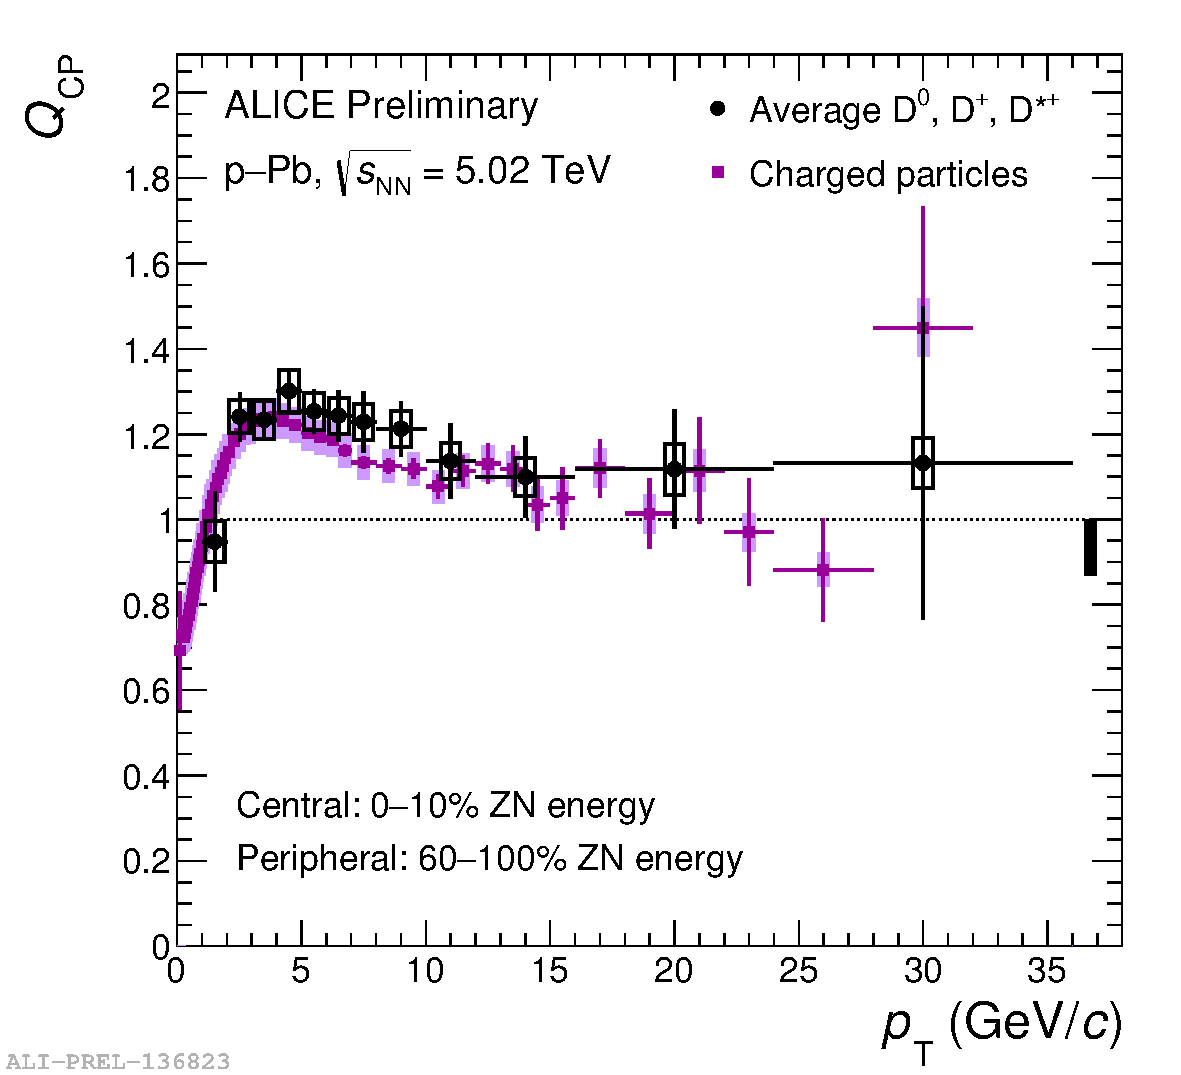
\includegraphics[width=8cm]{FigCap2/2017-Sep-12-QCP-Daverage-ChargedHadrons.pdf}
  \caption{D-meson (black) and charged-particle (magenta) central-to-peripheral nuclear modification factor~\cite{ALICEPAS2017008}.}
  \label{fig:RpA}
\end{figure}




The nuclear modification factor in p-Pb collisions can be also measured in given centrality classes.
Its definition is:
\begin{equation}
Q_{\rm pPb}^{\rm mult} = \frac{({\rm d}^2 N/{\rm d} \pt {\rm d} y)^{\rm mult}_{\rm pPb}}{\langle T_{\rm pPb} \rangle ^{\rm mult}({\rm d}^2 \sigma_{pp}/{\rm d} \pt {\rm d} y)},
\end{equation}
where $({\rm d}^2 N/{\rm d} \pt {\rm d} y)^{\rm mult}_{\rm pPb}$ 
is the yield of a given species in p-Pb collisions 
in a given centrality class, and $\langle T_{\rm pPb} \rangle ^{\rm mult}$ is the average nuclear 
overlap function in the same centrality class.
In order to achieve better precision on the yields, the ratio of the nuclear 
modification factor in central to peripheral events, $Q_{\rm CP}$, 
can be defined as:
\begin{equation}
Q_{\rm CP} = \frac{({\rm d}^2 N/{\rm d} \pt {\rm d} y)^{\rm central}_{\rm pPb}/ \langle T_{\rm pPb} \rangle^{\rm central}}{({\rm d}^2 N/{\rm d} \pt {\rm d} y)^{\rm peripheral}_{\rm pPb}/ \langle T_{\rm pPb} \rangle^{\rm peripheral}}.
\label{eq:QCP}
\end{equation}
The $Q_{\rm CP}$ of D mesons in the 0-10\% and 60-80\% 
centrality classes was measured by 
ALICE~\cite{ALICEPAS2017008} (Fig.~\ref{fig:RpA}, right panel) 
and it increases in the interval 1-4 $\Gevc$, 
up to values of about 1.25 and then tends to decrease. The 
average value of the D-meson $Q_{\rm CP}$ 
in the interval $3 < \pt < 8 \; \Gevc$ is larger than unity by 1.5 
standard deviations of the combined statistical and systematic uncertainty.
It is an open question whether the observed bump of $Q_{\rm CP}$, whose magnitude is similar 
for D mesons and charged particles, is related to initial state effects 
or to collectivity effects in the final state.
\iffalse
\begin{figure}[!ht]
  \centering
  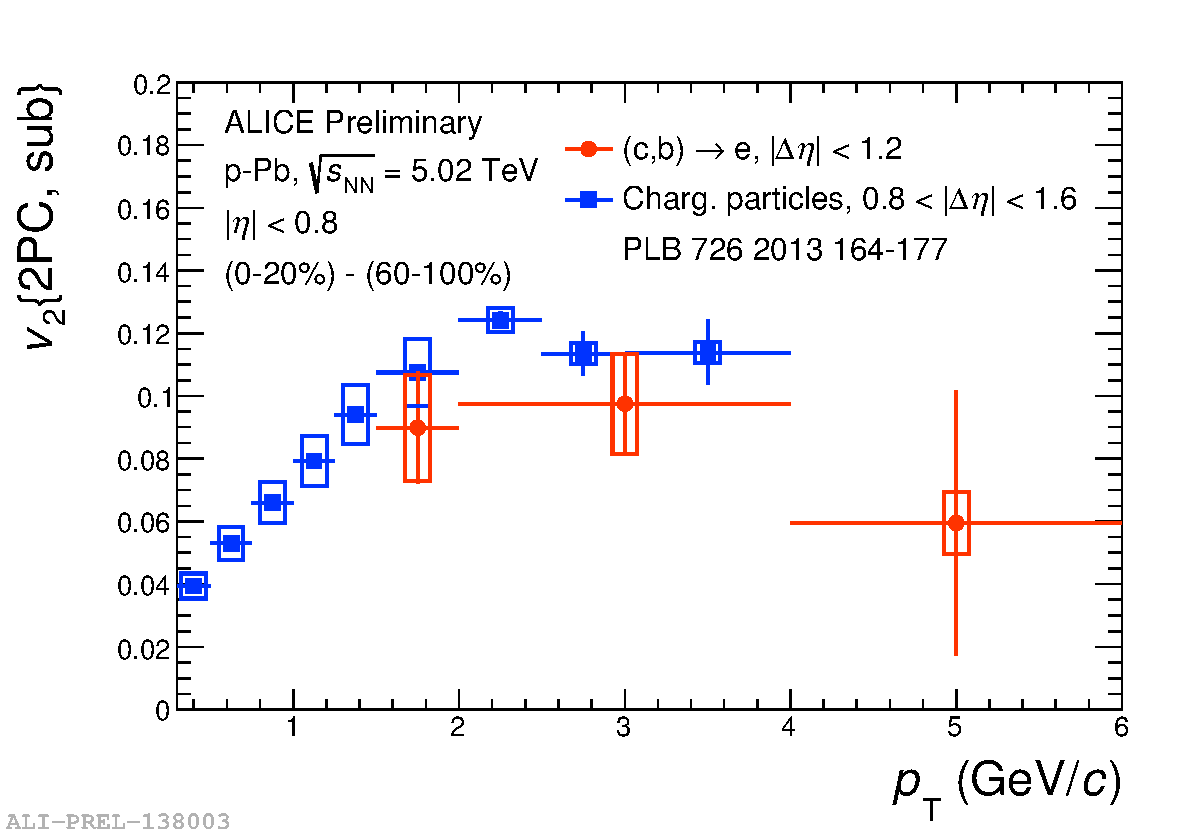
\includegraphics[width=7cm]{FigCap2/v2HFE.pdf}
  \caption{~\cite{Acharya:2017hdv}}
  \label{fig:}
\end{figure}
\fi
\section{Heavy quarks in A-A collisions}
\label{sec:HFEnLossinAA}
High-momentum partons traversing the QGP are expected 
to lose energy because of interactions 
with the medium constituents. One of the experimental observables 
used for the study of energy loss is the 
nuclear modification factor, defined in Sec.~\ref{sec:JetQuenching}. 
The possibility to disentangle
effects of cold nuclear matter from the ones related to in-medium 
energy loss paves the way to characterise the 
hot and dense medium properties. In fact, the magnitude of energy lost in the medium is
determined by the properties of the fireball like the transport coefficients,
that encode the momentum transfers with the medium, or the mean free 
path, closely related to the medium density $\rho$
and the cross section $\sigma$ of the parton-medium interaction. 
A colour charge can lose energy in a plasma at a temperature $T$ by two mechanisms: 
radiative and collisional energy losses, which originate, respectively, from elastic
and inelastic interactions with the medium constituents.
\subsection{Collisional processes}
\label{sec:coll}
Collisional processes are $2 \rightarrow 2$ elastic scatterings off thermal 
gluons (Fig.~\ref{fig:LoopCollScatt}, first to third diagrams) and quarks 
(Fig.~\ref{fig:LoopCollScatt}, fourth diagram). It is possible to calculate,
 in the limit $E \gg M^2/T$, the heavy-quark collisional energy loss 
 ${\rm d} E/{\rm d} x$ in a QGP, by summing all contributions of 
 Fig.~\ref{fig:LoopCollScatt}~\cite{Peigne:2008nd}:
\begin{equation}
\label{eq:QCDenLossColl}
\begin{split}
\frac{{\rm d} E}{{\rm d} x} = \; & \frac{4 \pi T^2}{3}\;  \alpha_s (m^2_D)\;  \alpha_s(ET) {\Big [} {\Big (}  1 + \frac{n_f}{6}{\Big )} {\rm ln} \frac{ET}{m^2_D} + \frac{2}{9} \frac{\alpha_s(M^2)}{\alpha_s(m^2_D)} \times {\rm ln} \frac{ET}{M^2}  \\+\;  &c(n_f) + \mathcal{O}{\Big (}\alpha_s (m^2_D) \; {\rm ln}\frac{ET}{m^2_D}{\Big )}{\Big ]},
\end{split}
\end{equation}
where $\alpha_s$ is the QCD running coupling constant, $n_f$ is the number of flavours 
considered in the scattering diagrams of Fig.~\ref{fig:LoopCollScatt} and $m_D$ is the 
Debye screening mass of the plasma $m_D = 4\pi \alpha_s T^2 (1 + n_f/6)$. 
\begin{figure}[!ht]
  \centering
  \includegraphics[width=14cm]{FigCap2/LO_HQscattering.png}
  \caption{Feynman diagrams for leading-order perturbative HQ scattering off light partons.}
  \label{fig:LoopCollScatt}
\end{figure}

The multiple scatterings of the heavy quark with the medium 
partons can also be treated as Brownian motion and is typically
be described by the Boltzmann equation. In the limit of small 
momentum transfer, the latter can be reduced to the 
Fokker-Planck equation, which is often further reduced into the
Langevin equation. These
partial-differential equations can be used as transport equations, 
to describe the evolution of the momentum distribution
of heavy quarks along time. The Langevin equation for heavy-quark 
collisional energy loss presents itself as~\cite{Cao:2013ita}:
\begin{equation}
\label{eq:Langevin}
\frac{{\rm d} {\vec{p}}}{{\rm d} t} = - \eta_D (p) \vec{p} + \vec{\xi}.
\end{equation}
In Eq.~\ref{eq:Langevin}, the first right-hand side term is the 
deterministic friction force, while the second one is the thermal random noise,
satisfying the properties:
\begin{equation}
\label{eq:Langevin2}
\langle {\xi^i (\pt)} {\xi^j (p_{\rm T'})} \rangle = b^{ij} (\pt) \frac{\delta_{tt'}}{{\rm d} t}, \; \; \; \; b^{ij} (\pt) = k_{\parallel}(p)\hat{p}^i\hat{p}^j + k_{\perp} (\delta^{ij} - \hat{p}^i\hat{p}^j).
\end{equation}
In Eq.~\ref{eq:Langevin2}, $k$ represents the momentum-space 
diffusion coefficient of heavy quarks;
the coefficient $\eta_D$ of Eq.~\ref{eq:Langevin2} is involved in the definition of the spatial 
diffusion coefficient $D_s$, which is related to the momentum-space 
diffusion coefficient via: 
\begin{equation}
\label{eq:Langevin3}
D_s = \frac{T}{M \eta_D} = \frac{2 T^2}{k}.
\end{equation}
To simulate the evolution of heavy quarks, one needs to discretise terms and calculate the increment 
$\vec{p}(t + \Delta t) -  \vec{p}(t)$ at a given time $t$. 

\subsection{Gluon-radiation processes}
\label{sec:rad}
While a parton is traversing the medium, it picks up some transverse 
momentum $k_{\perp}$ due to multiple scatterings. 
If we consider a gluon in the hard parton wave function, when the 
accumulated $k_{\perp}$ is enough, it can decohere from the partonic projectile and be emitted.
These are $1 \rightarrow 2$ processes, like $Q \rightarrow g\, Q$, 
where $Q$ is the heavy quark and $g$ the gluon.
The average phase $\phi$ of the gluon is approximately:
\begin{equation}
\label{eq:gluonPhase}
\phi = {\Big \langle} \frac{k_{\perp}^2}{2\omega} \Delta z {\Big \rangle} \sim \frac{\hat{q} L}{2 \omega} L = \frac{\omega_c}{\omega},
\end{equation}
where $\hat{q}$ is the transport coefficient of the medium, 
defined as the average squared transverse 
momentum transferred to the projectile per average unit path 
length $L$: $\hat{q} = \langle k_{\perp}^2 \rangle / L$ \cite{Salgado:2003gb,}.
Hence, gluons are emitted from the parton traversing a finite path 
length $L$ with a characteristic gluon frequency $\omega_c$:
\begin{equation}
\label{eq:gluonPhase}
\omega_c = \frac{1}{2} \hat{q} L^2.
\end{equation}
The distribution of energy $\omega$ of the radiated gluons, 
for small energies $\omega < \omega_c$ is of the form:
\begin{equation}
\label{eq:gluonEnDistrb}
\omega \frac{{\rm d} I}{{\rm d} \omega} \sim \frac{2 \alpha_s C_R}{\pi} \sqrt{ \frac{\omega_c}{2 \omega}},
\end{equation}
where $C_R$ is the Casimir factor for the QCD coupling, 
equal to 4/3 for quark-gluon coupling and to 3 for gluon-gluon coupling.
The $\omega$-integrated average parton energy loss results then:
\begin{equation}
\label{eq:RadEnLoss}
\langle \Delta E \rangle \propto \alpha_s \, C_R \, \hat{q} \, L^2. 
\end{equation}
We can then summarise the main properties of average parton 
energy loss via radiative processes:
\begin{itemize}
\item it grows with the path length like: $\Delta E \propto L^2$;
\item is proportional to $\alpha_s C_R$, thus it is larger by a factor 
9/4 $ = 2.25$ for a gluon traversing the medium than for a quark;
\item it is independent of the initial parton energy $E$.
\end{itemize}
Furthermore, while in the limit of massless partons the probability of 
gluon emission is maximum for collinear radiation,
in the massive limit the soft-gluon emission probability, for small 
emission angles $\Theta \ll 1$, is~\cite{Dokshitzer:1991fd}:
\begin{equation}
\label{eq:DeadCone}
{\rm d} \sigma_{Q \rightarrow gQ } \sim \frac{\Theta^2 {\rm d} \Theta^2}{[\Theta^2+ \Theta^2_0]} \frac{{\rm d} \omega}{\omega},
\end{equation}
with $\Theta_0 = M_Q/E_Q$.
Therefore, in the kinematical region $\Theta < \Theta_0$ the yield of radiated gluons
in the forward direction provides a small contribution to the total multiplicity. 
The depleted forward region is called the {\it dead cone}.
Since $\Theta_0 = M_Q/E_Q$, the effect is expected to be more 
relevant with increasing parton mass. A hierarchy in 
the energy loss is hence expected:
\begin{equation}
\label{eq:HierachyRaa}
\Delta E_{gluon} < \Delta E_{light\, quark} < \Delta E_{heavy\, quark},
\end{equation}
where the first inequality comes from the different couplings in $gg$ and $gq$ 
processes due to the Casimir factor in Eq.~\ref{eq:gluonEnDistrb} 
and the second from the dead-cone effect. The hierarchy, if present, 
should consequently affect the $\RAA$ values of hadrons originating from
gluon, light and heavy-quark fragmentation.\\


\begin{figure}[!ht]
  \centering
  \includegraphics[width=7cm]{FigCap2/HFEnLoss1.png}
  \includegraphics[width=7cm]{FigCap2/HFEnLoss2.png}
  \caption{Comparison of radiative and collisional energy losses for charm (left) and for bottom (right) quarks from calculations in~\cite{Cao:2013ita}.}
  \label{fig:HFEnLoss}
\end{figure}
In Fig.~\ref{fig:HFEnLoss}, an example of calculations from~\cite{Cao:2013ita}
for the energy loss of charm (left) and beauty (right) quarks 
in central Pb-Pb collisions at the LHC is shown as a function of the initial energy of the quark.
In the model~\cite{Cao:2013ita}, quarks evolve in a static medium at a temperature
$T = 300$ MeV according to a Langevin equation (like that in Eq.~\ref{eq:Langevin}) with 
an additional term for radiative contribution. 
Both the contributions from collisional and radiative energy loss 
are displayed in Fig.~\ref{fig:HFEnLoss}. Elastic interactions
dominate the low-$\pt$ region, up to $\sim 6\; \Gevc$ for charm and $\sim 16 \;\Gevc$ for beauty quarks.
At higher $\pt$, the contribution from radiative processes is the dominant one and must be considered when 
performing calculations at LHC energies.
It is also interesting to look at Fig.~\ref{fig:HFEnLoss2} (left), always from the
same calculations~\cite{Cao:2013ita}, that shows the 
thermalisation process of charm quarks in the medium as a function of time.
The initial energy of the charm quarks is 10 GeV. Depending on the different implementation for energy
loss, the thermalisation of the charm quarks occurs at different times.\\
\begin{figure}[!ht]
  \centering
  \includegraphics[width=7cm]{FigCap2/HFEnLoss3.png}
  \includegraphics[width=7cm]{FigCap2/FragHQ.png}
  \caption{Left: thermalization process of charm quarks in a static medium~\cite{Cao:2013ita}. Right: relative contributions from different hadronisation mechanisms to D-meson production  from charm quarks, as a function of the transverse momentum, from calculations in~\cite{Cao:2013ita}.}
  \label{fig:HFEnLoss2}
\end{figure}

\subsection{Heavy flavour hadronisation in the medium}
\label{sec:HFhadro}

The final hadron yields and momentum distributions depend not only on the energy loss 
mechanisms of the partons inside the medium,
but also on the way parton hadronisation occurs. There are basically 
two mechanisms for heavy quarks 
to produce heavy-flavour hadrons: fragmentation of a high-momentum 
heavy quark into a jet of lower-momentum
hadrons, or coalescence (re-combination) of low-momentum 
quarks with partons from the 
medium. Fig.~\ref{fig:HFEnLoss2} (right) illustrates the 
contributions of coalescence and fragmentation 
mechanisms into the final D-meson yields from charm-quark 
hadronisation in central Pb-Pb collisions at the LHC. The recombination mechanism
gives an important contribution at low $\pt$, while the independent 
fragmentation dominates at higher $\pt$.
Since the coalescence with partons from the medium gives rise to a 
hadron with momentum larger than that of the 
heavy quark, the $\pt$ distribution of the final hadrons produced via coalescence will be slightly 
harder than that of the initial quarks,
i.e. shifted towards higher momenta. A remarkable example
for the study of heavy-quark hadronisation processes is the production of J/$\psi$ meson,
discussed in Sec.~\ref{sec:Quarkonium}.\\



The measurement of $\Ds$-meson production in A-A collisions can provide 
crucial additional information for understanding the 
interactions of charm quarks with the strongly-interacting 
medium formed in heavy-ion collisions at high energies.
In particular, the $\Ds$-meson yield is sensitive to strangeness production 
and to the hadronisation mechanism of charm quarks.
The enhancement of strange particle production in presence of QGP was already discussed in
Sec.~\ref{subsec:StrangEnhancSPS} and a pattern of strangeness 
enhancement increasing with the hadron strangeness 
content when going from pp to p-A and then to heavy-ion collisions was observed at 
the SPS~\cite{NA57_158,NA57_40,NA49_Kpi,NA49_LambdaXi}, at
RHIC~\cite{STAR_hyperons} and at the LHC~\cite{ALICE:2017jyt}.
This strangeness enhancement effect could also affect the production of 
charmed hadrons if the dominant mechanism for D-meson formation at 
low and intermediate momenta is in-medium hadronisation of charm quarks via 
recombination with light quarks.
Under these conditions, the relative yield 
of $\Ds$ mesons with respect to non-strange charmed mesons at low $\pt$ is predicted to be enhanced
in nucleus-nucleus collisions as compared to pp 
interactions~\cite{Andronic2003,RafelskiKuznetsova,HeFriesRapp}.
The comparison of the $\pt$-differential production yields 
of non-strange D mesons and of $\Ds$ mesons in A-A and pp 
collisions is therefore sensitive to the role of recombination in charm-quark 
hadronisation.
\begin{figure}[!h]
  \centering
  \includegraphics[width=7cm]{FigCap2/RaaDsRapp.png}
  \includegraphics[width=7cm]{FigCap2/v2DsRapp.png}
  \caption{Results for the $\RAA$ (left panel) and $v_2$ (right) of $\Ds$ (red bands) and D (purple dashed-dotted lines) mesons in semi-central Au-Au collisions at RHIC~\cite{He:2012df},. Also results for charm quarks at pseudo-critical temperature $T_c$ (green dashed lines), the equilibrium limit for $\Ds$ meson mesons in the hydrodynamic medium at $T_{c}$ (blue dashed-double-dotted line) and STAR data for the D-meson $\RAA$ in in 0-80\% Au-Au~\cite{Zhang:2011uva}.}
  \label{fig:Rapp}
\end{figure}
Fig.~\ref{fig:Rapp} shows D- and $\Ds$-meson $\RAA$ (left-hand panel)
and $v_2$ (right), in semi-central Au-Au collisions at 
RHIC, from the TAMU model calculations~\cite{He:2012df}, also
compared to STAR measurements of D-meson $\RAA$ in 0-80\% Au-Au 
collisions~\cite{Zhang:2011uva}.
The model predicts the maximum $\RAA$ to be more 
pronounced for the $\Ds$, reaching values larger than 1.5 due 
to $c$-quark coalescence with the enhanced strangeness in Au-Au.
In the calculations of the model, the elliptic flow coefficient results to be sensitive both 
to the collectivity of the medium and to hadronization. Thanks to the coalescence of charm quarks with 
thermal light and strange quarks, the flow coefficients of non-strange D and $\Ds$ mesons reach
values larger by $\sim$50\% than the $v_2$ of charm quarks. Furthermore, interactions of non-strange D mesons
with the medium constituents during the hadronic phase create a further 30\%
difference between strange and non-strange D-meson $v_2$.

\iffalse
A consequence of the possibly enhanced production of $\Ds$ mesons in heavy-ion 
collisions would be a slight reduction of the fraction of charm quarks 
hadronising into non-strange meson species.
Therefore, the measurement of the $\Ds$-meson production is also relevant
for the interpretation of the comparison of the nuclear modification
factors of non-strange D mesons and light-flavour 
hadrons (pions)~\cite{ALICEDRAA,Adam:2015sza}, which is predicted 
to be sensitive to the quark-mass and colour-charge dependence of parton 
in-medium energy loss~\cite{ADSW,WHDG,Djordjevic}.
Furthermore, due to this possible modification of the relative abundances
of D-meson species, measuring the $\Ds$ yield at low $\pt$ is needed 
also to determine the total charm production cross section in Pb--Pb 
collisions.
\fi

\begin{figure}[!ht]
  \centering
    \includegraphics[width=7cm]{FigCap2/AverageDmesonRaa_010_DzeroSTAR_010.pdf}
    \includegraphics[width=7cm]{FigCap2/2017-Jul-05-DmesonAverage_010_3050_6080_comparison_04July2017.pdf}
  \caption{Left: average non-strange D-meson $\Raa$ as a function of $\pt$ in the 10\% most central Pb-Pb collisions at
 $\sNN=2.76$ TeVmeasured by ALICE~\cite{Adam:2015sza}, compared to $\Dzero$ $\Raa$ measured by the STAR Collaboration in Au-Au collisions at RHIC at
$\sNN=200$ GeV~\cite{Adamczyk:2014uip}. A zoomed-in plot of the interval $0 < \pt < 8\, \Gevc$ is shown in the inset. Right: average $\RAA$ 
  of prompt $\Dzero$, $\Dplus$ and $\Dstar$ mesons in the 0--10\% (red), 30--50\% (blue) and 60--80\% (black) centrality classes at $\sqrtsNN=5.02~\tev$~\cite{ALICE-PUBLIC-2017-003}.  }
  \label{fig:Raa}
\end{figure}

\subsection{Experimental results in A-A collisions}
\label{sec:resAAcap2}
In the left-hand panel of Fig.~\ref{fig:Raa}, the average D-meson $\RAA$ 
for the 10\% most central Pb-Pb collisions at $\sNN = 2.76$ TeV 
measured by ALICE~\cite{Adam:2015sza} is compared to the $\Dzero$ 
nuclear modification factor measured by the STAR Collaboration
for the 10\% most central Au-Au collisions at $\sNN = 200$ GeV~\cite{Adamczyk:2014uip}. 
The nuclear modification factors measured at the two energies are compatible within uncertainties for $\pt > 2\, \Gevc$.
Similar $\RAA$ of D mesons for $\pt > 5 \,\Gevc$ does not necessarily imply a similar charm-quark
energy loss at the two collision energies. A combined effect of a denser medium
and of the harder $\pt$ spectra at the LHC could result in similar values of $\RAA$ as at lower
collision energies~\cite{Baier:2002tc}. In the interval $1 < \pt < 2\, \Gevc$, the $\RAA$ 
measured by STAR shows a maximum. This effect can be described 
by models including parton energy loss, collective
radial flow and the contribution of the recombination mechanism to 
charm-quark hadronisation~\cite{Abelev:2006db}. The ALICE results at higher energy 
do not show a maximum. Several effects can explain differences at the two energies, 
due to the different role of initial-state effects or of radial flow at the 
two collision energies. In the initial state, the modification
of the parton distribution functions in a nuclear environment is predicted to lead
to a stronger suppression of the heavy-quark production yields at low $\pt$ with increasing
$\sNN$~\cite{Eskola:2009uj}, because of the smaller values of Bjorken-x probed. In addition, the 
$k_{\rm T}$-broadening effect, which gives rise to an enhancement of the $\RAA$ at low-intermediate
$\pt$ (Cronin peak), is known to be more pronounced at lower collision energies~\cite{Wang:1998ww,Vogt:2001nh}.
In the final state, in addition to energy loss, the collective expansion of the medium is
also predicted to affect the momentum distribution of charmed hadrons in heavy-ion collisions.
This effect could be enhanced by hadronisation via recombination.
The stronger radial flow at the LHC than at RHIC~\cite{Abelev:2008ab,Abelev:2013vea,Abelev:2012wca} does not necessarily give rise
to a more pronounced bump-like structure in the $\RAA$ at low $\pt$ with increasing collision
energy. Its effect can in fact be counterbalanced by the different shape of the momentum
spectra in pp collisions at different energies. Reduced uncertainties
on the measurements are needed to draw firmer conclusions.\\
Preliminaries results of the average nuclear modification factors 
of $\Dzero$, $\Dplus$ and $\Dstar$ as a function of
$\pt$ measured in Pb-Pb collisions at $\sNN = 5.02 $ TeV 
are shown in Fig.~\ref{fig:Raa} (left), 
for the 0--10\%, 30--50\% and 60--80\% centrality classes~\cite{ALICE-PUBLIC-2017-003}. 
The D-meson nuclear modification factors at $\sNN = 5.02$ TeV 
exhibit a suppression which is compatible within uncertainties 
with that measured at lower energy $\sNN = 2.76$ TeV~\cite{Adam:2015sza}. 
They show a suppression that is
maximal at $\pt=6$--$10~\gev/c$ for central and semi-central events, 
where a reduction of the yields by
a factor of about 5 and 2.5 with respect to the binary-scaled pp reference is observed 
in the two centrality classes, respectively.
The suppression decreases with decreasing $\pt$ for $\pt<6~\GeV/c$, and 
$\RAA$ is compatible with unity  in the interval $1<\pt<3~\gev/c$.
The average $\RAA$ in the 60--80\% centrality class shows a suppression 
by about 20--30\%, without a pronounced dependence on $\pt$. 
Recent studies proposed that event selections and geometry determination 
of the collision can affect $\RAA$ with a bias, causing
an artificial suppression for $\RAA$ in peripheral collisions even in absence
of jet quenching and shadowing~\cite{Morsch:2017brb}.\\


The $\RAA$ of prompt $\Ds$ mesons in the 10\% most central Pb-Pb collisions 
at $\sNN =  2.76$ TeV is compared in the right-hand panel
of Fig.~\ref{fig:Raa} to the average nuclear modification factor of 
$\Dzero$, $\Dplus$ and $\Dstar$ mesons measured in the same
centrality class~\cite{Adam:2015sza}. This comparison is meant to 
address the expected effect of hadronisation via quark
recombination in the partonic medium on the relative abundances 
of strange and non-strange D-meson
species. In the three $\pt$ intervals, the values of the $\Ds$-meson $\RAA$ 
are higher than those of non-strange D mesons, although 
compatible within the large uncertainties. More precise measurements are 
expected with the data sample from LHC Run 2 at $\sNN = 5.02$ TeV.\\
\begin{figure}[!ht]
  \centering
    \includegraphics[width=7.1cm]{FigCap2/RAADsD_276.pdf}
    \includegraphics[width=6.9cm]{FigCap2/2017-May-22-RaavsNpart_Dmes8to16_Pions8to16_FinalNonPromptJpsi2017_CC_25042017.pdf}
  \caption{Left: $\RAA$ of prompt $\Ds$ mesons~\cite{Adam:2015jda} compared to non-strange D mesons~\cite{Adam:2015sza} in the 0-10\% centrality class at $\sNN = 2.76$ TeV. Right: Comparison of the D-meson~\cite{Adam:2015nna} and charged-pion~\cite{Abelev:2014laa} $\RAA$ as a function of centrality expressed in terms of $\langle N_{\rm part} \rangle $ in 8 $< \pt < 16$ $\Gevc$~\cite{Adam:2015nna} 
and of the $\RAA$ of non-prompt J$/\psi$ mesons in 6.5 $< \pt < 30$ $\Gevc$ measured by CMS~\cite{Khachatryan:2016ypw}. 
}
  \label{fig:ColorMassDep}
\end{figure}

\begin{figure}[!ht]
  \centering
    \includegraphics[width=7.5cm]{FigCap2/2017-Jan-28-rParAAbeautyincl.pdf}
  \caption{Right: $\RAA$ of electrons from beauty-hadron decays as a function of $\pt$ together with
the corresponding result for beauty- and charm-hadron decays~\cite{Adam:2016khe} for the 20\% most central Pb-Pb collisions.}
  \label{fig:ColorMassDep}
\end{figure}

Fig.~\ref{fig:ColorMassDep} (left) shows the average of the $\Dzero$, $\Dplus$ and $\Dstar$ 
nuclear modification factors as a function of centrality measured by ALICE in
Pb-Pb collisions at $\sNN =  2.76$ TeV, for the interval 8 $< \pt < 16$ $\Gevc$~\cite{Adam:2015nna}, 
compared to the $\RAA$ of charged pions~\cite{Abelev:2014laa} in $|y| < 0.8$ for the same $\pt$ interval, 
and to non-prompt J$/\psi$ meson $\RAA$ measured by the CMS Collaboration for 6.5 $< \pt < 30$ $\Gevc$ 
in $|y| < 1.2$~\cite{Khachatryan:2016ypw}. The different width of the rapidity interval for D and non-prompt
J$/\psi$ mesons ($|y| < 0.5$ and $|y| < 1.2$, respectively) is not expected to play a big role, since
the intervals are partially overlapping and there is no significant $y$ dependence of the $\RAA$ of 
non-prompt J$/\psi$ mesons in $|y| < 1.2$~\cite{Khachatryan:2016ypw}. 
The $\pt$ interval 8-16 $\Gevc$ for D mesons was chosen 
in order to obtain a significant overlap with the $\pt$ distribution 
of B mesons decaying to J/$\psi$ particles with $6.5 < \pt < 30\, \Gevc$.
The nuclear modification 
factors of charged pions and D mesons are compatible within uncertainties
in all centrality classes. A possible interpretation of the similar $\RAA$ of D mesons and pions is 
related to a mixture of competitive effects which affect the nuclear modification
factor in addition to the parton in-medium energy loss. In particular,
in the presence of a colour-charge and quark-mass dependent 
energy loss, the harder $\pt$ distribution and the harder fragmentation function of 
charm quarks compared to those of light quarks and gluons could lead to similar 
values of D-meson and pion $\RAA$, as discussed in~\cite{Djordjevic:2013pba}. 
The value of the D-meson $\RAA$ in all the centrality
classes, except the most peripheral one, is lower than that of non-prompt J$/\psi$ mesons. 
The $\RAA$ of electrons from beauty-hadron decays~\cite{Adam:2016wyz} 
is compared with the one of heavy-flavour decay electrons, i.e. originating from both charm- and
beauty-hadron decays, in Fig.~\ref{fig:ColorMassDep} (right) 
for the 20\% most central Pb-Pb collisions
~\cite{Adam:2016khe}. The measurements agree within 
uncertainties at high $\pt$, while, in the $\pt$ 
interval 3 $< \pt < 6$ $\Gevc$, the $\RAA$ 
of electrons from beauty-hadron decays 
is about 1.2$\sigma$ higher than that of heavy-flavour decay 
electrons. The observation of different 
suppression for particles originating from
charm or beauty quarks like those presented in left- and 
right-hand panels of Fig.~\ref{fig:ColorMassDep} 
is consistent with a scenario of decreasing in-medium 
parton energy loss with increasing quark mass.

\begin{figure}[!ht]
  \centering
        \includegraphics[width=14cm]{FigCap2/D0v2_CMS_5TeV.png}
  \caption{Prompt $\Dzero$ meson $v_2$ (upper) and $v_3$ (lower) coefficients at midrapidity ($|y| < 1.0$) for
the centrality classes 0-10\% (left), 10-30\% (middle), and 30-50\% (right)~\cite{Sirunyan:2017plt}.}
  \label{fig:D0v2CMS}
\end{figure}

The measurement of the elliptic flow $v_2$ provides further 
insight into the interactions of charm quarks with the medium. 
At low $\pt$, D-meson $v_2$ offers the unique opportunity 
to test whether also charm quarks participate in the collective 
expansion dynamics and possibly thermalize in the medium~\cite{Greco:2003vf,Ollitrault:1992bk}. 
At low and intermediate $\pt$, the elliptic flow is also expected to 
be sensitive to the hadronization mechanism~\cite{Greco:2003vf}, while at high $\pt$, 
it can constrain the path-length dependence of parton energy loss~\cite{Gyulassy:2000gk}.
First measurements of a positive D-meson $v_2$ were done by ALICE
in Pb-Pb collisions at $\sNN = 2.76$ TeV~\cite{Abelev:2014ipa}.
The $v_2$ and $v_3$ of prompt $\Dzero$ meson measured by CMS 
in Pb-Pb collisions at $\sNN = 5.02 $ TeV are presented in 
Fig.~	\ref{fig:D0v2CMS}, for the 0-10\%, 
10-30\% and 30-50\% centrality classes ~\cite{Sirunyan:2017plt}. 
The measured $v_2$ and $v_3$ are larger than 0 
at low $\pt$ and then decrease at higher $\pt$.
The result suggests that charm quarks take part in 
the collective motion of the medium and that collisional interaction processes as well as quark 
recombination may contribute to the observed elliptic flow. 
For $\pt > 6\, \Gevc$, the $\Dzero$ meson $v_2 >0$ suggests a 
path-length dependence of the charm-quark energy loss. \\


\begin{figure}[!ht]
  \centering
    \includegraphics[width=7cm]{FigCap2/2017-Jul-07-DmesonAverage_010_All_Models_04July2017.pdf}
    \includegraphics[width=7cm]{FigCap2/DmesonAverage_3050_AllModels_18May2017.pdf}
    \includegraphics[width=7cm]{FigCap2/DmesonAverage_6080_All_Mod04July2017.pdf}
  \caption{Average D-meson $\RAA$~\cite{ALICE-PUBLIC-2017-003} in 0-10\%, 30-50\% and 60-80\% centrality classes as a function of $\pt$ at $\sNN = 5.02$ TeV, compared with models.}
  \label{fig:RAAandv2}
\end{figure}



\begin{figure}[!ht]
  \centering
    \includegraphics[width=11cm]{FigCap2/2017-Jul-04-DmesonComparisonWithModels.pdf}
%    \includegraphics[width=7cm]{FigCap2/2017-Sep-13-v2ESE_Daverage_PbPb3050_VZERO_q2TPCFullSmall60Perc_q2TPCFullLarge20perc.pdf}
  \caption{Average D-meson $v_2$~\cite{Acharya:2017qps} in the 30-50\% centrality class as a function of $\pt$ at $\sNN = 5.02$ TeV, compared with models.}
  \label{fig:RAAandv2}
\end{figure}

The simultaneous comparison of $\RAA$ and elliptic flow $v_2$ measurements 
with theoretical calculations can provide more stringent constraints to the 
charm-quark in-medium interactions and hadronisation processes.
A comparison is shown in Fig.~\ref{fig:RAAandv2} for the 
D-meson $\RAA$~\cite{ALICE-PUBLIC-2017-003} (left panel) 
and $v_2$~\cite{Acharya:2017qps} (right panel) measured
by ALICE in Pb-Pb collisions at $\sNN = 5.02$ TeV, in the 0-10\% and 30--50\% 
centrality classes respectively.
Transport models in Fig.~\ref{fig:RAAandv2} include: 
POWLANG~\cite{Beraudo:2014boa} and TAMU~\cite{He:2014cla}, 
in which the interactions only include collisional processes; 
BAMPS-el+rad~\cite{Uphoff:2014hza}, LBT~\cite{Cao:2017hhk} and 
PHSD~\cite{Song:2015ykw}, in which also energy loss from medium-induced gluon radiation
is considered, in addition to collisional process.
Models based on perturbative QCD calculations of parton energy loss 
are: CUJET3.0~\cite{Xu:2015bbz}, Djordjevic~\cite{Djordjevic:2015hra} 
and MC@sHQ+EPOS2~\cite{Nahrgang:2013xaa}, that include both radiative 
and collisional energy loss processes, and SCET~\cite{Kang:2016ofv} model, that includes 
medium-induced gluon radiation and a mechanism of formation and dissociation of 
heavy-flavour hadrons in the QGP. All models, with the exception of BAMPS and CUJET3.0, 
include a nuclear modification of the parton distribution functions.
The LBT, MC@sHQ, PHSD, POWLANG and TAMU
models include a contribution of hadronisation via quark recombination, 
in addition to independent fragmentation. 
Most of the models provide a fair description of the measured $\RAA$ in the region 
$\pt<10~\gev/c$ in central collisions, 
but many of them (LBT, PHSD, POWLANG and SCET) provide a worse 
description of non-central collisions.
%In the high-$\pt$ region above $10~\gev/c$ only the BAMPS, CUJET3.0, 
%Djordjevic and SCET models can describe the data. 
The CUJET3.0 and Djordjevic models provide a fair description of the $\RAA$ in all three 
centrality classes for $\pt > 5-10~\gev/c$, where radiative energy loss 
is expected to be the dominant interaction mechanism, suggesting that 
the dependence of radiative energy loss on the path length of charm 
quarks in the hot and dense medium is well understood. 
The TAMU model overestimates $\RAA$ at high $\pt$ in central events and describes 
the magnitude of the elliptic flow, but fails in reproducing the shape. This
may be due to missing radiative term for the energy loss. 
BAMPS-el overestimates the $v_2$ at low $\pt$ while underestimating the 
suppression at high $\pt$. The radiative term in BAMPS-el+rad improves the 
description of the $\RAA$ but gives a smaller than observed low $\pt$ 
$v_2$. POWLANG overestimates suppression at hight $\pt$ in all the centrality classes,
while gives a good description of the $v_2$.
~PHSD, LBT and MC@sHQ provide instead a fair 
description of both $v_2$ magnitude and shape
as well as of energy loss.\\





More quantitative comparisons between measurements and model
calculations towards an estimate of the heavy-quark transport coefficients
was proposed in a recent Bayesian model-to-data analysis~\cite{Xu:2017hgt}. 
The dependence of the charm quark diffusion coefficient 2$\pi T D_s(T)$ on the temperature 
(see Fig.~\ref{fig:DiffCoeff}) was extracted.
The spacial diffusion coefficient is better constrained in the region (1.3 - 1.5) $T_c$, that is indeed a 
temperature range where charm quarks spend most of their time in the medium.
Furthermore, the coefficient, extracted from model-to-data comparison, 
is found to be compatible to lattice QCD calculations and some results 
from the latter are displayed in Fig.~\ref{fig:DiffCoeff}.

\begin{figure}[!ht]
  \centering
    \includegraphics[width=10cm]{FigCap2/DiffCoeff.png}
  \caption{Estimated temperature dependence of the spatial diffusion coefficient  2$\pi T D_s(T)$, compared with other models calculations.}
  \label{fig:DiffCoeff}
\end{figure}



\chapter{The ALICE experiment at the LHC}
\label{chap:chap3}

\section{The Large Hadron Collider}
\label{sec:LHC}
The Large Hadron Collider (LHC), with a circumference of 27 km, 
is the world largest and most powerful particle collider, built by the 
European Organisation for Nuclear Research (CERN) from 1998 to 2008. 
It is placed in the tunnel of the previous Large Electron Positron collider, at a depth between 50 and 175 m underground.
The LHC accelerator chain is shown in Fig.~\ref{fig:imageLHC}. The first stage 
of the acceleration takes place on the Linac2, a linear accelerator with an 
output proton energy of 50 MeV. The proton-booster synchrotron (PSB) increases 
the energy to 1.4 GeV, injecting into the proton synchrotron (PS). This accelerates the
 beam to 26 GeV and injects it into the super proton synchrotron (SPS), out of which 
 450 GeV protons are eventually injected into the LHC for the start of the ramp up to 
 the energy of 7 TeV. At the nominal configuration, LHC accelerates protons grouped in 2808 bunches per beam, each bunch 
 containing up to $1.15^{11}$ protons. The beam is bent along the circular LHC 
 path by 1232 superconducting dipoles and controlled and focused by other 
 600 smaller magnets. The design and construction of the dipoles was the most 
 technologically challenging part of the accelerator. To achieve the required bending power, 
 the dipole field should be on average B $\sim$ 8.3 Tesla. The coils are made of 
 NiTi superconducting cable, kept at T = 1.9 K by superfluid liquid He. They are 
 15 m long, weigh 35 tonnes and store in their magnetic field 7 MJ of energy, for a total of 10 GJ in the full ring.\\
The nominal instantaneous luminosity for pp collisions, with a bunch crossing every 25 ns, is of $10^{34} {\rm s}^{-1} {\rm cm}^{-2}$; for 
Pb-Pb collisions it is about $10^{27} {\rm s}^{-1} {\rm cm}^{-2}$. Since September 2008, 
the four main experiments (ALICE, ATLAS, CMS and LHCb) collected data with pp
 collisions at $\s=900, 2.36, 2.76, 5, 7, 8$ and 13 TeV, 
 Pb-Pb collisions at $\sNN=2.76$ and 5.02 TeV, Xe-Xe collisions at $\sNN=5.44$ TeV and p-Pb collisions at $\sNN=5.02$ TeV.

\begin{figure}[!t]
\centering
\includegraphics[width=12cm]{FigCap3/CERN_Accl_Complex.png}
\caption{Layout of the full CERN accelerator complex, including all elements of the LHC injector chain.}
\label{fig:imageLHC}
\end{figure} 
\section{The ALICE experiment}
\label{sec:ALICE}
ALICE (A Large Ion Collider Experiment)~\cite{Abelev:2014ffa} is an experiment 
at the LHC optimised for the study of QCD matter
created in high-energy collisions between heavy nuclei.
The aim of ALICE is the study of the behaviour of matter at high densities and temperatures 
and at nearly zero baryo-chemical potential. 
The major challenge that the detector project had faced was the large number of 
particles created in Pb-Pb collisions. Moreover, the study of the QGP requires to reconstruct tracks down to
low momenta and identify them on a wide momentum range.
For this reason, ALICE detectors were designed to have a 
high granularity, a low transverse momentum threshold $\pt^{\rm min} \sim 0.15 $ 
$\Gevc$ and good particle identification capabilities up to 20 $\Gevc$.
The apparatus consists of three main parts: 
\begin{itemize}
\item \textbf{central barrel}, contained within the large magnet producing a moderate solenoidal 
field of B = 0.5 T in nominal running conditions and composed of detectors devoted to the reconstruction of charged particles, photons
and jets and covering the pseudo-rapidity range -0.9 $< \eta <$ 0.9 over the 
full azimuth. They are the Inner Tracking System (ITS), optimised for vertex 
reconstruction and tracking; a cylindrical Time Projection Chamber (TPC),
 surrounding the ITS, that is the main detector for tracking and provides also particle identification; a 
 Transition Radiation Detector (TRD), designed for electron identification; 
 a Time Of Flight (TOF) detector, that provides pion, proton and kaon 
 identification; a Photon Spectrometer (PHOS); an Electromagnetic 
 Calorimeter (EMCal) and a Di-Jet Calorimeter (DCal), a High-Momentum Particle IDentification (HMPID) 
 and the ALICE Cosmic Ray Detector (ACORDE);
\item \textbf{forward muon spectrometer}, dedicated to the study of 
muons in the pseudo-rapidity range $2.5< \eta < 4.0$;
\item \textbf{the forward detectors}, which include the Photon Multiplicity Detector 
(PMD) and the silicon Forward Multiplicity Detector (FMD), dedicated to the 
measurement of photons and charged particles around $|\eta| \sim 3$, respectively; 
the quartz Cherenkov T0 detector, which delivers the time and the longitudinal
 position of the interaction; the plastic scintillator V0 detector, which measures 
 charged particles at -3.7 $< \eta <$ -1.7 and 2.8 $< \eta <$ 5.1, and is mainly used
  for triggering and for the determination of centrality and event plane angle in 
  Pb-Pb collisions; the Zero Degree Calorimeter (ZDC) also used for determination of centrality.
\end{itemize}
The layout of ALICE set-up is shown in Fig.~\ref{fig:imageALICE}. 
\begin{figure}[!t]
\centering
\includegraphics[width=12cm]{FigCap3/alice.png}
\caption{Picture of the ALICE experiment detectors.}
\label{fig:imageALICE}
\end{figure}
ALICE apparatus has overall dimensions of 16 x 16 x 26 m$^3$ and a total 
weight of $\sim$10000 t. The maximum pp interaction rate at which all ALICE 
detectors can be safely operated is around 700 kHz. Typical luminosity values 
for the ALICE pp data taking range from \textit{L} $\sim 10^{29}{\rm s}^{-1}{\rm cm}^{-2}$ 
to \textit{L} $\sim 10^{31}{\rm s}^{-1}{\rm cm}^{-2}$.
In the following sections, the detectors of ALICE used in the analyses presented in this thesis and their 
performance will be described. For information on the other detectors more details can be found in~\cite{Aamodt:2008zz}.

\subsection{Magnet}
\label{sec:Magnet}
The magnet used in ALICE was constructed for the L3 experiment at LEP and 
it produces a moderate solenoidal magnetic field (B $<$ 0.5 T). In the choice 
of the magnetic field two aspects must be considered: the magnet has to be intense 
enough to bend the particle trajectory and allow a good track-momentum resolution, 
but has to permit the reconstruction of low 
momentum particles. The lower momentum that allows reconstruction of the track 
with the ALICE magnet is given by $p_{\rm cutoff}=$ 0.3$\,$B$\,$R $\sim 0.2\,\Gevc$, 
where B is the magnetic field in Tesla and R is the minimum radius for a particle to 
traverse the entire TPC, whose external radius is R$_{\rm ext}=$ 2.5 m.
Tracks with lower momentum can be reconstructed using the Inner tracking System, as discussed
in the next sections.

\begin{figure}[!t]
\centering
\includegraphics[width=8cm]{FigCap3/figures_its-rf-2.png}
\caption{View of the six silicon layers of the Inner Tracking System}
\label{fig:image2}
\end{figure}

\subsection{Inner Tracking System (ITS)}
\label{sec:ITS}
The Inner Tracking System is one of the central barrel detectors used for track 
reconstruction, primary and secondary vertex finding and Particle Identification (PID).
It is composed by six cylindrical layers of silicon detectors placed 
coaxially around the beam vacuum tube (Fig.~\ref{fig:image2}). The layers are located 
at radii between 39 mm and 430 mm and cover the pseudo-rapidity range 
$|\eta|<0.9$. The two innermost layers are made of Silicon Pixel Detectors (SPD). 
The pseudo-rapidity coverage of the SPD inner layer is $|\eta|<1.95$ for particles produced at $\zVtx=0$. 
The two middle layers are made of Silicon Drift Detectors (SDD) 
and two outer layers of Silicon micro-Strip Detectors (SSD).
Its basic functions are~\cite{ITS-TDR}:
\begin{itemize}
\item determination with high precision of primary vertex position (interaction point) and reconstruction of secondary vertices 
of charm, beauty and hyperon decays,
\item improvement of the momentum and angle measurements of the TPC,
\item recover particles that are not tracked in the TPC due to acceptance limitation (very low momentum particles
not reaching the TPC and high momentum particles crossing the inactive areas between adjacent TPC chambers).
\end{itemize}
All the ITS detectors were carefully optimised to minimise their radiation 
 length, achieving 1.1\% per layer, the lowest value among all the current LHC experiments~\cite{ITS-TDR}. 
The resolution of the track impact parameter is determined by the spatial resolution of 
the ITS detectors. The ITS detectors have a spatial resolution of a few tens of 
$\mu$m in the $r\varphi$ plane, with the best precision (12  $\mu$m) for the 
innermost detectors equipped with SPD. The left and the right panels of Fig.~\ref{fig:VtxResolDCAResol}, that will be discussed
 in Sec.~\ref{sec:tracking}, show respectively the resolution on the final vertex position in transverse coordinates and on the impact parameter
in the transverse plane. \\
 
 \begin{figure}[!h]
\centering
\includegraphics[width=.65\textwidth]{FigCap3/ITSpid.png}
\caption{Distribution of the energy-loss signal in the ITS as a function of momentum. The lines show the parameterisations of the expected mean energy loss.}
\label{fig:imagePIDITS}
\end{figure}

 The four outer layers provide analogue read-out and for this reason they 
 can be used for particle identification (PID) via d$E$/d$x$ measurements for 
 low-$\pt$ particles. The measured cluster charge in each of the four layers with PID capabilities is normalised to the path length
 in the silicon active volume, 
 which is calculated from the reconstructed track parameters, to obtain a d$E$/d$x$ 
 value for each layer. A single d$E$/d$x$ value is then calculated with a truncated mean of
 the values from the four layers, to assure that
 the d$E$/d$x$ peak shape is Gaussian. 
  The resolution $\sigma$ on the d$E$/$x$ is of about 10\% and it provides kaon-pion
 separation at 1$\sigma$ level for $\pt \lesssim 0.7 \, \Gevc$ and proton/pion separation 
 for $\pt \lesssim 1.2 \, \Gevc$.
 An example of the distribution of the measured truncated mean values of energy loss 
 per path unit as a function of track momentum in the ITS is shown 
 in Fig.~\ref{fig:imagePIDITS}. 
 \begin{figure}[!h]
\centering
\includegraphics[width=.6\textwidth]{FigCap3/TPC.png}
\caption{A view of the ALICE Time-Projection Chamber detector.}
\label{fig:imageTPC}
\end{figure}

\subsection{Time Projection Chamber (TPC)}
\label{sec:TPC}
The TPC is the only device which can provide good tracking
performance up to track densities of 8000 charged particles per unit of rapidity, 
which were foreseen to be produced in Pb-Pb collisions at the LHC at the time when
ALICE was designed~\cite{Dellacasa:451098}. 
It has a cylindrical shape with inner and outer radius of 80 and 250 cm, 
respectively, and an overall length in the beam direction of 500 cm. The minimum  
inner radius of the TPC was determined by the maximum acceptable hit density. 
The outer radius was defined by the minimum length required for a d$E$/d$x$ resolution 
better than 10\%. At smaller radii (and larger track densities), tracking is taken over 
by the ITS. The TPC covers an acceptance of $|\eta|<0.9$. The TPC is a chamber full of 
high-purity gas to transport ionisation electrons over long distances (2.5 m) towards the read-out end-plates. 
It is composed by a central high-voltage (HV) electrode which divides the 
gas volume into two symmetric drift regions, and two opposite axial potential degraders to
create a highly uniform electrostatic field of up to 400 V/cm (Fig.~\ref{fig:imageTPC}).
Charged particles traversing the gas form a ionisation trace that will move at constant 
velocity towards one of the two end-plates. The density of ionisation depends on the velocity and mass of the particle.
Once on the end-plate, readout chambers allow to amplify and register the signals 
of particle tracks. The end-plates are segmented into 18 trapezoidal sectors 
and equipped with multi-wire proportional chambers covering an overall active area of 32.5 $m^2$.
The original mixture of gas was composed by 90\% Ne, 10\% ${\rm CO}_2$; successively a further 5\% of N$_2$
was added. During 2015-2016, the Ar replaced the Ne in the mixture.
 \begin{figure}[!h]
\centering
\includegraphics[width=.65\textwidth]{FigCap3/TPCpid.png}
\caption{Distribution of the energy-loss signal in the TPC as a function of momentum. The lines show the parameterisations of the expected mean energy loss.}
\label{fig:imagePIDTPC}
\end{figure}
The TPC is the main detector for track reconstruction (see Sec.~\ref{sec:tracking}). 
It is used for measurements of the charged-particle 
momenta, with a resolution better than 2.5\% for electrons with momentum 
of about 4 $\Gevc$, and for particle identification via d$E$/d$x$.\\


Particle Identification is performed over a wide momentum range. It is made by 
simultaneously measuring the specific energy loss, the charge and the momentum of the 
particles traversing the detector gas. The maximum number of clusters associated to a track in the TPC 
is 159 and the d$E$/d$x$ value of the track is determined using a truncated mean.
The d$E$/d$x$, described by the Bethe Block formula,
is parameterised by a function proposed by ALEPH Collaboration~\cite{Rolandi:2008qla}:
\begin{equation}
f(\beta_\gamma) = \frac{P_1}{\beta^{P_4}} \Big ( P_2 - \beta^{P_4} - {\rm ln}\Big (   P_3 + \frac{1}{(\beta_\gamma)^{P_5}} \Big )   \Big ),
\end{equation}
where $\beta$ is the particle velocity, $\gamma$ is the Lorentz factor, and $P_{1-5}$ are fit parameters. 
The measured d$E$/d$x$ as a function of the track momentum measured in TPC is
shown in Fig.~\ref{fig:imagePIDTPC}. The lines correspond to the parametrisation. 
A clear separation among the different particle species
is observed for $\pt \lesssim 1 \, \Gevc$, which allows for a PID on a track-by-track basis. At higher $\pt$ the separation of the species is still feasible 
on a statistical basis via multi-Gaussian fits. The PID resolution is about 5.2\% in 
pp collisions and 6.5\% in the 5\% most central Pb-Pb collisions. Thanks to the d$E$/d$x$ resolution, 
particle ratios can be measured in the relativistic rise region at $\pt$ up to $\approx 20\, \Gevc$.
 \begin{figure}[!h]
\centering
\includegraphics[width=.5\textwidth]{FigCap3/TOFCylinder.png}
\caption{A view of the ALICE Time-Of-Flight detector.}
\label{fig:imageTOF}
\end{figure}

\subsection{Time-Of-Flight (TOF)}
\label{sec:TOF}
The TOF detector is a large area array of Multigap Resistive Plate Chambers (MRPC), 
positioned at radial distance of 370-399 cm from the beam axis. It has a cylindrical 
shape, covering polar angles between 45 and 135 degrees over the full azimuth. 
The TOF has a modular structure with 18 sectors in $\varphi$ (Fig.~\ref{fig:imageTOF}); each 
of these sectors is divided into 5 modules along the beam direction. 
This detector is entirely devoted to particle identification. 
The ionisation produced by any particle crossing the MRPCs starts a gas avalanche 
which generates the observed signal. The TOF identifies the particle species via a measure of the time of flight 
inside the chambers. Let us consider the following relation:
\[
m = p \sqrt{\frac{t^2_{\rm TOF}}{L^2}-1}
\]
where $m$ is the mass of the particle, $p$ the momentum, $t_{\rm TOF}$ the time-of-flight and 
$L$  the track length. It can be shown that the $\sigma_m/m$ resolution, at relatively high
 momenta, it is influenced much more by the errors on the time-of-flight and track length 
 measurements than by error on the momentum determination.
 The time of collision, which constitutes the start time for the time-of-flight measurement,
 is obtained on an event-by-event basis either using the particle arrival times
 at the TOF, or the information from the T0 detector, or a combination of the two~\cite{Adam:2016ilk}. 
 The T0 detector is composed by two arrays of
Cherenkov counters, T0A and T0C, located at apposite sides of the interaction point at 
$-3.28 < \eta < - 2.97$ and $4.61 < \eta < 4.92$. It has a time resolution of 20-25 ps
 in Pb-Pb collisions and $\sim 40$ ps in pp collisions.
 The TOF resolution is 80 ps for pions with a momentum around 1 $\Gevc$, in 0-70\% Pb-Pb collisions.
This values includes the detector resolution, the contribution from electronics and the uncertainty
on the start time of the event.
It provides PID in the intermediate momentum range, allowing for pion/kaon separation at 3$\sigma$ level
up to $\pt \approx 2.5 \,\Gevc$  and kaon/pion separation up to $\pt \approx 4 \,\Gevc$.
Figure \ref{fig:TOFpid} shows the distribution of the measured velocity $\beta$ as a function of momentum (measured by TPC). 
The background is due to tracks that are incorrectly matched to TOF hits in high-multiplicity Pb-Pb collisions.
\begin{figure}[!h]
\centering
\includegraphics[width=.7\textwidth]{FigCap3/TOFpid.png}
\caption{Distribution of $\beta$ velocity measured by the TOF detector as a function of momentum for particles reaching the
TOF in Pb-Pb interactions.}
\label{fig:TOFpid}
\end{figure}


\subsection{V0 Detector} 
\label{sec:V0}
The V0 detector is made of two arrays of scintillator counters, V0A and V0C, positioned on both sides of 
the interaction point. The V0A detector is located at 340 cm distance from the nominal interaction point position, 
along the beam axis, on the side opposite to the muon spectrometer,
whereas V0C is fixed to the front face of the hadronic absorber, 90 cm from the nominal interaction point. They cover
the pseudo-rapidity ranges $2.8 < \eta < 5.1$ (V0A) and $-3.7 < \eta < -1.7$ (V0C) and are segmented
into 32 individual counters each distributed in four radial rings and 8 azimuthal sectors. 
The V0 provides a minimum bias trigger as well as high-multiplicity triggers for the central barrel detectors and
  can be used to estimate the centrality of the collision based on the energy deposited in the V0 scintillator tiles.
Furthermore, it is used for beam-gas background rejection (see Sec.~\ref{sec:BkgRejection}).


\subsection{Zero Degree Calorimeter (ZDC) Detector} 
\label{sec:ZDC}
The ZDC provides a measure of the energy carried in the forward direction (at 0$^\circ$ relative
to the beam direction) by non-interacting (spectator) nucleons. This quantity is
useful to estimate the centrality of the event. Typically the beams are deflected by means 
of two separation dipoles located at about 65 m distance from the interaction point (IP). These magnets will also deflect the spectator
 protons, separating them from the spectator neutrons, which fly away at 0$^\circ$. 
Two sets of ZDCs are placed at about 115 m distance from the 
 interaction point on both sides of the interaction point. Each set is constituted by one 
 calorimeter for neutron detection (ZN), positioned between the two 
 beam vacuum tubes to intercept the spectator neutrons, and one for proton detection (ZP), placed externally 
 to the outgoing beam, to collect the spectator protons. 
  The hadronic ZDCs are quartz-fibre sampling calorimeters. The shower generated by incident
particles in a dense absorber (tungsten for ZN and brass for ZP) produces 
Cherenkov radiation in quartz fibres (the active material) interspersed in the absorber.
The two sets of ZDCs are complemented by the information of two small 
electromagnetic calorimeters (ZEM), located at 7.5 m from the interaction
 point, to detect the  energy of particles emitted at forward rapidity (mainly photons generated from $\pi^0$ decays).




\section{The ALICE Trigger System and Data Aquisition}
\label{sec:trigger}
ALICE has a two-layer trigger architecture~\cite{Fabjan:684651}. The low-level trigger is a 
hardware trigger called Central Trigger Processor (CTP). The High-Level trigger (HLT)
 is implemented as a pure software trigger. 
The ALICE Central Trigger Processor (CTP) is designed to combine and synchronise 
information from all the triggering detectors in ALICE and informations about the LHC filling scheme and
bunch crossing, and to send the correct sequences
 of trigger signals to all detectors. Since the ALICE 
 experiment has to collect data in pp (p-Pb) and Pb-Pb collisions, the trigger system was optimised 
 for these two types of collisions. The HLT allows the implementation of sophisticated 
 logic for the triggering. While the CTP governs the readout of the sub-detectors, the 
 HLT receives a copy of the data read out from the sub-detectors and processes it.

\subsection{The Central Trigger Processor (CTP)}
\label{sec:CTP}
The hardware trigger combines informations from sub-detectors to decide whether or 
not to write an event on disk. The CTP evaluates trigger inputs from the trigger detectors every machine clock cycle ($\sim25$ ns). 

The trigger inputs are divided into three different levels:
\begin{itemize}
\item L0 level: the Level 0 trigger decision (L0) is made $\sim 0.9\, \mu$s after the 
collision using V0, T0, EMCal, PHOS, and MTR. The trigger requirement can be 
simply the input of one detector or a logical condition based on the trigger 
inputs of different trigger detectors.
\item L1 level: the events accepted at L0 are further evaluated by the Level 1 (L1) 
trigger algorithm in the CTP. The L1 trigger decision is made $\sim 6.5\, \mu$s after L0. 
The latency is caused by the computation time (TRD and EMCal) and propagation times 
(ZDC, 113 m from IP2). The L0 and L1 decisions, delivered to the detectors with a 
latency of about 300 ns, trigger the buffering of the event data in the detector front-end electronics. 
\item L2 level: the Level 2 (L2) decision, taken after about 100 $\mu$s corresponding to the 
drift time of the TPC, triggers the sending of the event data to DAQ and, in parallel, to the High Level Trigger system (HLT). 
L2 can be used to reject events with multiple collisions (pile-up) in different bunch crossings occurring
in the TPC readout time.
\end{itemize}
Information about the LHC bunch filling scheme is used by CTP to suppress the background. 
The information about the bunch crossing, regarding the arrival of bunches from both A-side and C-side,
or one of them, or neither, is provided to the CTP by the bunch crossing mask at a resolution of 25 ns. 
The beam-gas interaction background, can be studied by triggering on bunches without a collision partner, and can be 
subtracted from the physics data taken with the requirement of the presence of both bunches.
ALICE operates with minimum-bias (MB) triggers, mainly based on V0 and SPD, 
and with rare triggers that are optimised to select particular classes of events such as 
events containing jets or muons or high-multiplicity events. By definition MB triggers 
have the highest rate of inputs signals, while the rare triggers have much lower rate. 
In general, several types of triggers during the data taking at the same time keep busy a 
very large fraction of the total data acquisition bandwidth. To prevent losing precious events due to the fact that no 
space is available on the temporary memory, the trigger system follows an event prioritisation scheme. 
In the case that the utilisation of the temporary storage is above a certain 
value, only rare triggers are accepted. This scheme significantly increases the acceptance of rare events.

\subsection{The Data AcQuisition System (DAQ)}
\label{sec:DAQ}
The DAQ manages the data flow from the sub-detector electronics to the archiving
 on tape. Once the CTP decides to register a specific event, raw data are sent to 
 the Local Data Concentrators (LDCs) via the optical Detector Data Links (DDLs). 
 LDCs are sets of computers that perform sub-event reconstruction. In this step of 
 the acquisition, raw data are processed. The size of a single central event processed 
 by LDCs can be $\approx$70 MB. In order to optimise the usage of the recording bandwidth available, 
 an additional event selection and compression is done by the High-Level Trigger (HLT).
The events processed by LDCs are then transferred to a second layer of computers, the Global Data Collectors 
 (GDCs), which perform the event building.
  
 \subsection{The High Level Trigger (HLT)}
\label{sec:HLT}
The ALICE software trigger, called HLT, is a farm of multiprocessor computers. 
It is composed by about 1000 PCs processing the data in parallel allowing an 
online analysis of the events. The HLT receives a copy of the raw data for events passing the L2 trigger level
and performs per-detector reconstructions. The trigger decision is based on 
the global reconstructed event, hence from a much more complete 
information than that available for the hardware trigger. Therefore, the HLT allows for more 
sophisticated triggers. Examples include triggers on high-energy jets or on muon pairs. 
Data rate reduction is achieved by reducing the event rate by selecting interesting events 
(software trigger) and by reducing the event size by selecting sub-events (e.g. pile-up 
removal in pp interactions) and by advanced data compression. In particular,
the data volume produced by the TPC is reduced via the HLT by reconstructing 
clusters or hits and by storing cluster information instead of the raw data.
The trigger decision, partial readout information, compressed data, and the reconstruction output is sent to LDCs and 
subsequently processed by the DAQ. 

\section{Machine-induced background}
\label{sec:BkgRejection}
The operation of detectors at the LHC can be affected by machine-induced
background (MIB), that scales with the beam intensity. The sources of this background can be: (i) beam-gas interactions,
caused by nucleons in the beams interacting with residual gas in the beam pipe;
(ii) interactions of the beam halo with mechanical structures in the machine; (iii)
collisions of bunches in the main radio-frequency buckets with satellite bunches located at short 
distance from the main bunches. 
The background from sources (i) and (ii) can be rejected by exploiting the arrival time of the signal in the two V0 module detectors.
The background caused by one of the LHC beams produces in fact an early
signal on one of the two V0 (depending on the side from where the beam arrives) 
compared to the collision time at the nominal interaction point.
The difference between the expected beam and background signals 
is about 22.6 ns in the A side and 6 ns in the C side. As shown in the left panel of Fig.~\ref{fig:V0sumdiff}, 
background events accumulate mainly in two peaks at (-14.3 ns, -8.3 ns)
and at (14.3 ns, 8.3 ns) in the V0 time sum-difference plane, 
well separated from the main (collision) peak at (8.3 ns, 14.3 ns). 
\begin{figure}[!h]
\centering
\includegraphics[width=.49\textwidth]{FigCap3//V0sumdiff.png}
\includegraphics[width=.49\textwidth]{FigCap3//SPDcltsVsTcklts.png}
\caption{Left: correlation between the sum and difference of signal times in 
V0A and V0C. Right: correlation between reconstructed SPD clusters and tracklets. The green dashed line is used to separate
the populations of collisions and MIB.}
\label{fig:V0sumdiff}
\end{figure}
The V0 time information is 
used to set the trigger conditions on collision or background events. 
The collected events are further selected offline to remove any residual
contamination from MIB and satellite collisions.
The V0 trigger logic is re-applied at the offline level using a V0 arrival time 
computed offline as a weighted average of all detector elements.
For pp collisions, an additional selection on the correlation
between number of hits and track segments (tracklets) in SPD detector is used.
In fact, background particles usually cross the pixel layers in a 
direction parallel to the beam axis, producing hits that are not associated 
to any tracklet in the reconstruction (right panel of Fig.~\ref{fig:V0sumdiff}).
The dashed green line represents the cut used in the offline selection: 
events lying in the region above the line are tagged as background and rejected.
The fraction of background events that survives the above cuts was determined
by control triggers with only one of the beams crossing the ALICE 
interaction point and was found to be about 0.3\% in the pp data taking 
during the 2010 run, but it strongly depends 
on the running conditions and on the specific trigger configuration under study. 
In Pb-Pb collisions the fraction was found to be smaller than 0.02\%.
Collisions of main bunches and satellite bunches located at short 
distance from the main bunch are also a source of background. 
They are rejected using the correlation between the sum and the difference 
of times measured in the ZDC, as shown in Fig.~\ref{fig:ZNAselection} for Pb-Pb collisions.
The large cluster in the middle corresponds to collisions between ions 
in the main bunches, while the small clusters along the diagonals (spaced by 
2.5 ns in time difference) correspond to collisions in which one of the ions belongs
to satellite bunches.
\begin{figure}[!h]
\centering
\includegraphics[width=.49\textwidth]{FigCap3/ZNAselection.png}
\caption{Correlation between the sum and the difference of times recorded by the neutron ZDCs on either side (ZNA and ZNC) in Pb-Pb collisions. }
\label{fig:ZNAselection}
\end{figure}

\section{Electromagnetic interactions}
\label{sec:EMB}
The study of the properties of QGP requires to focus on the hadronic interactions in heavy-ion collisions.
At LHC energies, the cross sections for electromagnetic (EM) processes are very large ($\mathcal{O}$(kbarn)).
They are due to ultra-peripheral collisions between the EM clouds of the two colliding ions that can occur via 
(i) ultra-peripheral $\gamma \gamma$ collisions, (ii) photo-nuclear interactions.
The first process generally results in the creation of an $e^+e^-$ pair.
Photo-nuclear interactions are generated by one photon from the EM field of one of the nuclei
that interacts with the other nucleus, possibly fluctuating into a vector meson. 
In particular, among photo-nuclear processes, there is the electromagnetic dissociation (EMD), in which the sudden EM pulse
produced by the crossing ions leads to the dissociation of one (single) or both (mutual) nuclei
with the emission of at least one nucleon (neutron).
The single EMD events can be rejected by correlating the response of ZNA and ZNC.
In general, the selection of events with multiplicity larger than a certain threshold (see Sec.~\ref{sec:centr})
allows the rejection of EM processes.

\section{Track and vertex reconstruction}
\label{sec:tracking}
The track reconstruction and vertex finding are performed offline using information of the central
barrel detectors (ITS and TPC). The track reconstruction is based on the Kalman filter~\cite{Fruhwirth:1987fm}, which performs
simultaneously the track recognition (track finding) and reconstruction (track fitting). The main steps are described below.
\begin{itemize}
\item {\bf Clusterisation step:} the detector data are converted into ''clusters'' (i.e. groups of hits produced by the 
same particle crossing the considered detector element) characterised 
by positions, signal amplitudes, signal times, etc., and their associated errors. The clusterisation 
is performed separately for each detector. 
\item {\bf First interaction vertex reconstruction with SPD:} the clusters found in the SPD detector are used to determine the tracklets,
i.e. segments of tracks build by associating pairs of reconstructed points close in azimuthal angle ($\Delta \varphi <$ 0.01 rad) and 
pseudo-rapidity in the two SPD layers.
The preliminary vertex is defined as a space point where the maximum number of tracklets converge.
In pp collisions, where interaction pileup is expected, the algorithm is repeated several times, discarding at 
each iteration those clusters which contributed to already-found vertices. When a primary vertex is not found 
(particularly in low-multiplicity events) or in Pb-Pb collisions, the algorithm performs a one-dimensional 
search in the $z$-distribution of the points of closest approach of tracklets to the nominal beam axis.
\item {\bf TPC track finding and inward propagation:} track finding and fitting is performed in three stages, following an inward-outward-inward scheme.
The first inward stage starts with track finding in the TPC. The TPC can produce a maximum of 159 clusters per track
(corresponding to its 159 tangential pad rows). The track finding procedure starts at large TPC radius.
Track seeds are built with two TPC clusters and the interaction point reconstructed from the SPD tracklets, then with three clusters 
and without the vertex constraint. The track seeds are propagated inward with the Kalman filter algorithm and, at each step, 
the nearest cluster is added. A special algorithm is used to reject tracks with a fraction of common clusters
larger than a certain limit (between 20\% and 50\%). Only tracks that have at least 20 clusters (out of the maximum 159)
and that miss no more than 50\% of the clusters expected for a given track position are accepted. 
The contamination from tracks with more than 10\% wrongly associated clusters does not exceed 3\%
even in most central Pb-Pb collisions.
The efficiency of tracking in TPC is defined as the ratio between the reconstructed tracks 
and the generated primary particles in the simulation, and is shown in Fig.~\ref{fig:TPCtrackEffAndME} (left) as a function of 
the transverse momentum of the track. The tracking efficiency steeply drops below $\pt \sim 0.5 \, \Gevc$
due to the interaction of the particles with the detector material. The efficiency is almost 
independent of the occupancy in the detector. 
\begin{figure}[!h]
\centering
\includegraphics[width=.49\textwidth]{FigCap3/TPCtrackEff.png}
\includegraphics[width=.49\textwidth]{FigCap3/ITSTPCmatchEff.png}
\caption{Left: TPC track finding efficiency for primary particles in pp collisions at $\s=8$ TeV and Pb-Pb collisions at $\sNN=2.76$ TeV(simulation)~\cite{Abelev:2014ffa}. Right: track prolongation efficiency from TPC to ITS as a function of $\pt$ for data and Monte Carlo in Pb-Pb collisions at $\sNN=2.76$ TeV~\cite{Abelev:2014ffa}.}
\label{fig:TPCtrackEffAndME}
\end{figure}
\item{\bf Track inward propagation to ITS:} the reconstructed tracks in the TPC are propagated inward towards the ITS,
matching them to clusters in the outermost ITS layers. They are then propagated inwards and updated at each ITS layer attaching 
all clusters that satisfy a proximity cut. Each TPC track is hence associated to a tree of tracks in the ITS.
The track candidates in ITS are then selected with quality cuts (reduced $\chi^2$ and number of shared clusters with
other tracks). The tracks are then extrapolated to their point of closest approach to the IP reconstructed with SPD 
tracklets. The track prolongation efficiency from TPC to ITS, also called matching efficiency, in Pb-Pb collisions is shown in Fig.~\ref{fig:TPCtrackEffAndME} (right),
as a function of $\pt$ of the tracks for different requests on ITS points. 
The prolongation efficiencies from data and Monte Carlo (MC) simulations are shown by solid and open symbols, respectively. 
\item{\bf Standalone ITS track finding:} since the track efficiency in TPC allows to reconstruct tracks down to $\pt \sim 200$ MeV/$c$ for pions 
and $\pt \sim 400$ MeV/$c$ for protons, a standalone ITS reconstruction is performed with those clusters 
that were not used in the ITS-TPC tracks. The used algorithm allows to track low-momentum particles 
down to e.g. $\pt \sim 80$ MeV/$c$ for pions. The standalone ITS tracking allows also to recover
high-$\pt$ particles crossing the TPC in the active regions between adjacent chambers.
\item{\bf Track outward propagation:} the Kalman filter is used to propagate the tracks 
in the outward direction using the clusters found at the previous stage. 
The tracks are matched to TRD tracklets
in each of the six TRD layers, if possible, and to TOF clusters. The track length integral 
and the time of flight expected for various particle species are updated for 
subsequent particle identification with TOF. The matching with outer detectors (EMCal, PHOS and HMPID)
is also attempted. Only the TPC and the ITS points are used to update the measured track kinematics.
\item{\bf Final inward propagation (refit):} in the last step of the track reconstruction procedure, 
the tracks are propagated inwards starting from the outer radius of the TPC. 
The tracks are refitted in TPC and ITS with the previously found clusters and finally are propagated
to their distance of closest approach to the interaction point determined from SPD tracklets. 
The position, direction, curvature of the track (proportional to the inverse of transverse momentum)
and its associated covariance matrix are determined.  
\item{\bf Interaction vertex reconstruction with tracks:} ITS-TPC tracks are used to find the interaction vertex position 
with a higher precision than with SPD tracklets. The resolution on the transverse ($x,y$) position of the interaction vertices 
found with SPD and with global tracks are shown in the left panel of Fig.~\ref{fig:VtxResolDCAResol}. 
Both resolutions scale with the square root of the number of contributing tracks (tracklets).
The resolution of the distance of closest approach to the 
primary vertex in the transverse plane for charged-particle ITS-TPC tracks in pp, p-Pb and Pb-Pb collisions is shown in Fig.~\ref{fig:VtxResolDCAResol} (right). 
The resolution improves in heavier systems thanks to large multiplicities that allow a more precise 
determination of the primary vertex. The relative transverse-momentum resolution of the tracks is related to the
resolution on the track curvature via:
\begin{equation}
\label{eq:ptResol}
\frac{\sigma_{p_{\rm T}}}{\pt} = \pt \, \sigma_{1/p_{\rm T}}.
\end{equation}
The inverse-$\pt$ resolution for TPC standalone tracks and ITS-TPC combined tracks 
is shown in Fig.~\ref{fig:PtResolAndSecVtxResol} (left), for p-Pb collisions as a function of the inverse $\pt$.
In central Pb-Pb collisions, the $\pt$ resolution deteriorates by $\sim 10-15\%$ at high $\pt$.
\begin{figure}[!h]
\centering
\includegraphics[width=.49\textwidth]{FigCap3/VtxReso.png}
\includegraphics[width=.49\textwidth]{FigCap3/DCAxyResol.png}
\caption{Left: resolution on the transverse coordinate of the vertex position from tracks (solid points) and SPD tracklets (open points) as a function of multiplicity~\cite{Abelev:2014ffa}. Right: resolution of the distance of closest approach to the primary vertex in the transverse plane for charged ITS-TPC tracks. The contribution from the vertex resolution is not subtracted~\cite{Abelev:2014ffa}. }
\label{fig:VtxResolDCAResol}
\end{figure}
\end{itemize}
\begin{figure}[!h]
\centering
\includegraphics[width=.49\textwidth]{FigCap3/ptResol.png}
\includegraphics[width=.49\textwidth]{FigCap3/vertexSec.pdf}
\caption{Left: $\pt$ resolution for TPC standalone and ITS-TPC tracks with and without the constraint to the vertex~\cite{Abelev:2014ffa}. Right: resolution of the position of the reconstructed secondary vertex of $\DplustoKpipi$ decays along $\Dplus$ $\pt$ direction (black), 
orthogonal to $\Dplus$ $\pt$ direction (red), and along $z$-axis (blue).}
\label{fig:PtResolAndSecVtxResol}
\end{figure}

\section{Secondary vertex reconstruction}
\label{sec:secVertex}
For the reconstruction of heavy-flavour hadron decays, the reconstruction of decay vertices 
is done during the analysis phase. Tracks are grouped in pairs (e.g. for the $\DtoKpi$ decays) or in triplets (for the $\Dplus$ and $\Dsplus$ cases), 
defining objects called ``candidates''. 
The algorithm used for the secondary vertex reconstruction is based on a straight 
line approximation of the tracks (which are helices) in the vicinity of the primary vertex, by calculating the tangent line.
The algorithm finds the point of minimum distance between the two (or three) tracks by minimising the quantity:
\begin{equation}
D^2= \sum_{i=1}^N d_i^2,
\end{equation}
where N is the number of decay particles (3 in case of $\DstoKKpi$ decays) and $d_i$ is the distance between the track $i$ and the vertex 
($x_0$, $y_0$, $z_0$), weighted with the errors from the track covariance matrix:
\begin{equation}
d^2_i=\left(\frac{x_i-x_0}{\sigma_{x_i}}\right)^2+
\left(\frac{y_i-y_0}{\sigma_{y_i}}\right)^2+\left(\frac{z_i-z_0}{\sigma_{z_i}}\right)^2.
\end{equation}
The resolution of the reconstructed secondary vertex is shown in Fig.~\ref{fig:PtResolAndSecVtxResol} (right) 
(right) as example for the $\DplustoKpipi$ meson. The 
resolution improves with increasing $\Dplus$ meson $\pt$ and is better in the plane perpendicular to the $\Dplus$ $\pt$ direction.
The resolution of the secondary vertex for the $\DstoKKpi$ meson is similar to that of $\Dplus$.
Resolutions of about 100 $\mu$m allow to resolve the $\Ds$ decay vertices, which are
displaced from the interaction point by $\approx 150-300\,\mu$m.


\section{Simulations}
\label{sec:simu}
Simulations are used in the analysis to calculate the reconstructed efficiencies and to study the detector
performance.
Event generators are used to simulate pp, p-Pb and Pb-Pb collisions. In particular, PYTHIA 6 and
PYHTIA 8 were used for pp collisions, DPMJET, HIJING and EPOS-LHC for Pb-Pb and p-Pb collisions
for the studies presented in this thesis.
The physics processes at partonic level and informations such as type, momentum, 
charge, mother/daughter relationships... are stored in the kinematics tree. The GEANT package
is then used to simulate the transport of the particles through the
  detectors. During the transport, the energy deposition in the various detectors is stored 
  as ''hits''. The hits are subsequently converted into ''digits'', which represent 
  the real detector response and take into account instrumental effects, such as the presence of inactive channels, the noise 
  due to the front-end electronics ... The digits correspond to the raw data coming from the 
  Data Acquisition System in a real data taking. The same reconstruction procedure used for real data is applied to the simulated
  digits.

\section{Centrality determination}
\label{sec:centr}
The geometrical Glauber model~\cite{Miller:2007ri} introduced in Sec.~\ref{sec:glauber} describes
nuclear collisions as a superposition of binary nucleon-nucleon interactions. 
A participant nucleon of one nucleus is defined as a nucleon that undergoes one or more 
 collisions with nucleons of the other nucleus. The number of participants nucleons $N_{\rm part}$
 can be calculated as a function of the impact parameter $b$ of the collision using the Glauber
 model, the nucleon-nucleon inelastic cross section and the nucleon density profiles of the projectile and target
 nucleus. The number of spectator nucleons can be computed from the number of participant nucleons 
$N_{\rm part}$ as $N_{\rm spec}$ = $A_{\rm proj}$ + $A_{\rm target}$ - $N_{\rm part}$, where $A_{\rm proj}$ and $A_{\rm target}$
are the mass numbers of the colliding nuclei. The number of binary 
collisions $N_{\rm coll}$ can be calculated for a given value of the impact parameter. 
The impact parameter $b$ and other geometry-related quantities ($N_{\rm part}$, 
$N_{\rm spec}$, $N_{\rm coll}$) are not directly measurable. The determination of the collision centrality is based 
measurements of multiplicity (energy) produced in the collision, which can be described utilising
the Glauber model convoluted with a model for particle production based on a negative binomial distribution (NBD):
\begin{equation}
\label{eq:NBD}
P_{\mu, k} (n) = \frac{\Gamma(n+k)}{\Gamma(n+1)\Gamma(k)}\frac{(\mu/k)^n}{(\mu/k+1)^{n+k}},
\end{equation}
which gives the probability of measuring $n$ hits per independent emitting source of particles (called ancestor),
 where $\mu$ is the mean multiplicity per ancestor and $k$ controls the width of the distribution. 
The number of ancestors is parameterised as: $N_{\rm ancestors} = fN_{\rm part} + (1- f) N_{\rm coll}$.
This is inspired by two-component models~\cite{Deng:2010mv,Kharzeev:2004if}, which decompose particle production in nucleus-nucleus 
collisions into the contributions due to soft and hard interactions, where the soft interactions produce particles with 
an average multiplicity proportional to $N_{\rm part}$, and the probability for hard interactions to occur is proportional to $N_{\rm coll}$. 
\begin{figure}[!h]
\centering
\includegraphics[width=.52\textwidth]{FigCap3/v0glau_276.pdf}
\includegraphics[width=.46\textwidth]{FigCap3/zdczem.pdf}
\caption{Left: distribution of the sum of amplitudes in the V0 scintillators for events in Pb-Pb collisions at $\sNN=2.76$ TeV~\cite{Abelev:2013qoq}. The distribution is fitted with the NBD-Glauber fit, shown as a red line. The centrality classes used in the analysis are indicated in the figure. The inset shows a zoom of the most peripheral region. Right: spectator energy deposited in the ZDC calorimeters as a function of ZEM amplitude~\cite{Abelev:2013qoq}. The lines are a fit to the boundaries of the centrality classes with linear functions.}
\label{fig:centrality}
\end{figure}
%Two experimental observables related to the collision geometry are the average charged-particle 
%multiplicity $\Nch$ and the energy carried by particles close to the beam direction and 
%deposited in zero-degree calorimeters (ZDC). The average charged-particle multiplicity decreases
%monotonically with the impact parameter. 
With the Glauber Monte Carlo approach, the collision processes are simulated  
and the $N_{\rm part}$, $N_{\rm coll}$ and the number of ancestors are computed event by event. 
This allows to extract multiplicity distributions which can be compared to the measured ones and to extract the values of the parameters
$\mu, n $ and $k$.
The standard method typically used in ALICE is to define 
the centrality classes in Pb-Pb collisions based on the NBD-Glauber fit to the sum of V0A and V0C amplitudes. 
Other methods are used to asses the systematic uncertainty on the centrality determination~\cite{Abelev:2013qoq}.
In Fig.~\ref{fig:centrality} (left panel) the distribution of the V0 amplitudes for Pb-Pb collisions 
at $\sNN=2.76$ TeV~\cite{Abelev:2013qoq} is shown. The events were triggered with a signal in both V0A
and V0C and at least two hits in the outer SPD layer. The beam background was removed,
as well as part of the EM background with a ZDC cut and a $z$-vertex cut ($|\zVtx|<10$ cm).
The V0 amplitude obtained with the NBD-Glauber model fitted to the data is shown as a red curve
 in Fig.~\ref{fig:centrality} (left). The centrality is expressed as a percentage of the total nuclear interaction cross section
$\sigma$ obtained by integrating the V0
amplitude distribution. The normalisation is performed utilising the integral up to a threshold value V0$_{\rm THR}$ (anchor point), which corresponds
to the 90\% of the total hadronic cross section. For example, if we define V as the VZERO amplitude, 
the top 10\% central class is defined by the boundary V0$_{10}$ which satisfies:
\begin{equation}
\label{eq:percentileV0}
\frac{\int_{{\rm V0}_{\rm 10}}^\infty ({\rm d }N_{\rm ev} / {\rm d}V) {\rm d}V}{\int_{{\rm V0}_{\rm THR}}^\infty ({\rm d }N_{\rm ev} / {\rm d}V) {\rm d}V} = \frac{1}{9}.
\end{equation}
 Events with lower multiplicity than that of the anchor point
suffer from contamination of EM background and trigger inefficiencies, therefore are not used
in the determination of the centrality percentiles. The experimental distribution can be divided into classes by defining intervals on the measured distribution, 
which correspond to defined percentile intervals of the hadronic cross section. 
Another detector that can be used to determine the centrality of an event is the ZDC.
The energy deposited by the spectator nucleons in the ZDC has a monotonic dependence
on the multiplicity only for relatively small impact parameter values. For peripheral collisions, in particular,
it is possible that the nuclei fragments resulting from the collision have a magnetic rigidity (ratio
of their charge and mass) similar to that of beam particles, thus they are not bent away from the beam vacuum tube 
by the magnets and their energy is not
collected by the ZDCs. For this reason, the ZDC information needs to be correlated with the signals measured
by the two EM calorimeters (ZEM), as shown in the right panel of Fig.~\ref{fig:centrality}~\cite{Abelev:2013qoq}. 
The centrality classes previously determined 
by using the V0 are used to individuate the centrality classes in the ZDC-ZEM plane, since the ZEM
amplitude has unknown dependence on $N_{\rm part}$ and $N_{\rm coll}$. Then, the centrality classes 
are defined by cutting the plane into regions defined by straight lines from linear fits to the boundary regions
between two adjacent classes. This allows to define centrality intervals up to the 30\% of the hadronic cross section,
but not for more peripheral collisions.


\section{The ALICE Offline Software Framework}
\label{sec:offline}
In ALICE, pp and Pb-Pb events recorded with MB trigger have an average size of about 1.1MB and 13.75 MB respectively. 
For the Pb-Pb data sample at $\sNN=5.02$ TeV in 2015, a total raw data volume of 2.4 PB was collected; volumes of 500 TB and 2.7 PB
of raw data were collected for the p-Pb (2016, $\sNN=5.02$ TeV) and pp (2017, $\s=13$ TeV) data samples, respectively.
 The processing and analysis of these data necessitate 
unprecedented amount of computing and storage resources. Grid computing provides 
the answer to these needs. Grid computing consists of a coordinated use of large sets 
of different, geographically distributed resources in order to allow high-performance 
computation. It is organised in different levels or Tiers. Data coming from LHC experiments 
are stored in the CERN computing centre, the Tier-0. Copies of the collected data are then 
replicated in large regional computing centres (Tier-1), which also contribute in the event 
reconstruction and Monte Carlo simulation. Tier-2 centres are computing centres located
 in different institutions which do not have large storage capabilities but provide a large 
 fraction of the computing resources for Monte Carlo simulations and 
 data analysis. ALICE uses the ALICE Environment (AliEn) system~\cite{Saiz:2003wi} as a 
 user interface to connect to a Grid composed of ALICE specific services that are part 
 of the AliEn framework and basic services of the Grid middleware installed at the different sites.

\subsection{The AliRoot Framework}
\label{subsec:AliRoot}
The ALICE offline framework, AliRoot~\cite{Aamodt:2008zz} is based on Object-Oriented techniques
 for programming and, as a supporting framework, on the ROOT system~\cite{Brun:1997pa}, 
 complemented by the AliEn system which gives access to the computing Grid. The 
 AliRoot framework was developed as an extension of ROOT and is used for simulation, 
 alignment, calibration, reconstruction, visualisation and analysis of the experimental data.
\begin{figure}[h]
\centering
\includegraphics[width=10cm]{FigCap3/aliroot.png}
\caption{Schematic view of the AliRoot framework.}
\label{fig:aliroot}
\end{figure}
The AliRoot framework is schematically shown in Fig.~\ref{fig:aliroot}. The STEER module 
provides steering, run management, interface classes, and base classes. The detector related software is divided in 
independent modules that contain the code for simulation and reconstruction. Detector response simulation can be performed 
via different transport  packages like GEANT3~\cite{Brun:1082634} 
written in FORTRAN and GEANT4~\cite{Agostinelli:2002hh} written in C++. In these packages 
the detector material budget is simulated in detail, including support structures and 
the beam pipe. The transport code can hence simulate the decays of unstable 
particles and the trajectory of the daughter particles, the interactions of the 
particles with the detectors material and the production of secondary particles.
The reconstruction results are stored in ESDs (Event Summary Data), from which 
the AODs (Analysis Object Data) are extracted. The AODs contain the relevant information
for physics analyses. Additional information, used only for some specific analysis, is stored in additional
files, usually called delta-AODs. For example, specific AOD are produced for the 
reconstruction of open-charm meson with two or three body decays.
The analysis code, which contain the tasks utilised by the user to read the AOD files on the GRID and
to produce quantities, histograms and trees for final analysis, calculations of efficiencies and quality and
stability checks, is contained in the AliPhysics framework, which is built on the AliRoot and ROOT
frameworks and is progressively developed by the data analysis groups.

\chapter{$\Dsplus$ production in pp collisions at $\s$ = 7 TeV}
\label{chap:pp}
The 7 TeV sample is the one providing up to now the most precise pp reference for
the nuclear modification factors $\RAA$ and $\RpPb$. 
Furthermore, it constitutes a benchmark for pQCD predictions
at this energy.
In comparison to previous ALICE publications based on the same data 
sample~\cite{ALICE:2011aa,Abelev:2012tca,Adam:2016ich}, the present 
results~\cite{Acharya:2017jgo} have total uncertainties reduced by a factor of about two. This improvement 
has several sources: 
\begin{itemize}
\item changes in the detector calibration, alignment and track reconstruction 
algorithm, which resulted in better $\pt$ resolution, thus higher signal-to-background ratio; 
\item optimization of the D-meson selection procedure; 
\item refinements in the estimation of the systematic uncertainties, which is now more data-driven;
\item a data sample with 20\% larger integrated luminosity.
\end{itemize} 
Events are selected requiring a primary vertex reconstructed from ITS+TPC tracks with 
$z$-vertex coordinate $|z_{\rm RecoVert}|<~10$~cm, 
and pile-up events are rejected.  
The number of analysed events is 370M, while it was 300M for the previous reconstruction.

\section{$\Dsplus$ reconstruction and strategy}
\label{sec:DsRecoStrategy}
The transverse momentum spectra of prompt charm-strange $\Dsplus$ meson 
was measured in the rapidity range $|y| < $0.5 in pp collisions at 
$\sqrt{s}$ = 7 TeV with the ALICE detector.\\
The $\Dsplus$ mesons can not be directly detected because of 
their mean proper decay length $c\tau = 150\pm 2$ $ \mu$m~\cite{Olive:2016xmw} 
that prevent them from reaching the detectors. Hence, the analysis is 
based on the reconstruction of the full decay chain.
$\Dsplus$ mesons and their antiparticles were 
 reconstructed in the decay channel $\Dstophipi$ 
 (and its charge conjugate) followed by $\PhitoKK$ 
 (Fig.~\ref{fig:DsDecayTopology}). The branching ratio (BR) of this decay channel 
 is 2.27 $\pm$ 0.08 \%~\cite{Olive:2016xmw}.
Other $\Dsplus$ decay channels can give rise to the same final products
 $\KKpi$, such as $\Dsplus\rightarrow {\rm  K^{*0} K^+}$ and 
 $\Dsplus\rightarrow f_o(980) \pi^+$ with BR  2.63 $\pm$ 0.13 \% and 
 1.16 $\pm$ 0.32 \%, respectively. It was verified that the selection efficiency for 
 these decay modes is strongly suppressed by the cuts applied 
 to select the signal candidates of $\DstophipitoKKpi$, that include 
 a selection exploiting the mass of the intermediate resonant state. 
 Since the width of the $\phi$ peak is narrower than those of the 
 K$^{*0}$ and the $f_o(980)$, the decay channel through the 
 $\phi$ resonance, being the one that provides the best discrimination 
 between signal and background, was used in this analysis. 
 The $\Dsplus$ signal is extracted from 
 the invariant-mass\footnote{The invariant mass equation is \\ 
 \begin{align*} m^2 =& E^2 -\vec{p}^{\, 2} = (E_1 + E_2)^2 -(\vec{p_1} + \vec{p_2})^2 \\ m^2 =& m_1^2 +m_2^2 + 2(E_1E_2 -p_1p_2cos\theta) \end{align*}} 
 distribution of the candidates, which are obtained by 
 combinatorial association of three reconstructed tracks with the correct 
 charge-sign combination. Hence, 
 the invariant-mass distribution will have a contribution from real 
 $\Dsplus$ decays ($\DstoKKpi$) and an other 
 from combinatorial background of uncorrelated tracks. In order to have a reduction of the
  background, specific cuts were applied on the decay topology, on
   the invariant mass of $\KK$ pair and on the particle identification, 
   as explained in the following sections. 
$\Dsplus$ meson mean proper decay length of $\sim 150\, \mu$m  
makes it possible to separate their decay vertex from the primary vertex
of the pp interaction. 
This gives a fundamental contribution in rejecting tracks which do not come from a displaced vertex.
\begin{figure}[!t]
\centering
\includegraphics[width=12cm]{FigCap4/Ds.png}
\caption{Schematic view of the $\Dsplus\rightarrow \phi \pi^+ \rightarrow K^+K^-\pi^+$ decay.}
\label{fig:DsDecayTopology}
\end{figure}
Before the candidates go through specific selections of the decay
topology and particle identification, they have to pass single-track 
quality cuts. In the following, details of each selection step will
be illustrated. 



\section{Single-track selections}
Reconstructed tracks were selected by requiring:
\begin{itemize}
\item pseudo-rapidity $|\eta| < 0.8$
\item minimum $\pt > 0.3~\GeV/c$
\item at least 70 (out of a maximum of 159, i.e. number of TPC pad rows) 
associated space points in the TPC
\item $\chi^2/\mathrm{ndf} < 2$ in the TPC (where ndf is the number of degrees of 
freedom involved in the tracking procedure)
\item at least two (out of six) hits in the ITS, out of which at least one 
in either of the two SPD layers
\item ratio of crossed rows (total number of hit TPC pad rows, i.e. corrected 
for pad rows with missing signal) over findable clusters (pad rows which, 
based on the geometry of the track, are possible clusters) in the TPC larger than 0.8
\end{itemize}
For tracks that satisfy the above selection criteria, the transverse momentum 
resolution is better than 1$\%$ at $\pt = 1\, \Gevc$ and about 2\% at $\pt = 10 \, \Gevc$. 
The resolution on the track impact parameter, which is the distance of closest 
approach of the track to the primary vertex, is better than 75 $\mu$m for 
$\pt >$ 1 $\Gevc$ for the projection on the bending plane ($r\phi$, normal to 
the beam direction) in pp collisions.
In order to have unbiased determination of the primary vertex, for each 
$\Dsplus$ candidate the interaction point was recalculated from the reconstructed 
tracks after excluding the candidate decay tracks.
\begin{figure}[!htbp]
\begin{center}
\includegraphics[width=.5\textwidth]{FigCap4/YvsPt.png}
\label{fig:singtrafter}
\caption{Rapidity versus $\pt$ distribution of the reconstructed $\Dsplus$ mesons. The fiducial acceptance region is defined by $|y| < y_{fid}(\pt)$.}
\end{center}
\end{figure}

The single-track selection criteria reduce the $\Dsplus$-meson acceptance, which drops 
steeply to zero for $|y| > 0.5$ at low $\pt$ and for $|y| > 0.8$ 
at $\pt > 5~\Gevc$. A $\pt$-dependent fiducial acceptance region was therefore defined as 
$|y| < y_{\mathrm{fid}}(\pt)$, with $y_{\mathrm{fid}}(\pt)$ increasing 
from 0.5 to 0.8 in the transverse momentum range $0 < \pt < 5~\Gevc$ 
according to a second-order polynomial function, and $y_{\mathrm{fid}}=0.8$ 
for $\pt > 5~\Gevc$.

\section{Decay-chain and topology selection}

The single-track selection provids a certain number of candidate
 decay tracks. Then, $\Dspm$ candidates are build from combinatorial 
 association of three candidate tracks, with the correct combination of charge 
 sign. In this way, a huge number of candidates is created, most of them 
 being combinatorial background. The goal is to separate background from
  $\Dspm$ signals (i.e. corresponding to real  $\Dspm$ decays). Candidates 
  are thus selected by applying topological cuts, specific to the meson and its 
  decay channel and varying as a function of the D-meson $\pt$.
The main feature of the $\Dsplus$-decay topology is the presence of three tracks displaced from 
the primary vertex and compatible with the hypothesis of being originated from 
a common point. 
The variable that allows one to evaluate the displacement of a track is the 
impact parameter. The two most important detectors for the measurement
 of the impact parameter are the two SPD inner layers of the Inner Tracking System. \\
Below, the topological cuts used for $\Dspm$ signal selection
 are explained in detail. Fig.~\ref{fig:var1},~\ref{fig:var2} and~\ref{fig:var3} complement
 the description, showing distributions of some of the below listed variables
 for signal and background candidates, in the interval $2 < \pt < 16 \, \Gevc$, 
 extracted from Monte Carlo production (PYTHIA~\cite{Sjostrand:2006za}) and data, respectively.
  New topological variables were introduced with respect to the 
  previous analysis of this sample. They are the projections of the cosine of 
the Pointing angle and of the (normalised) decay length in the $xy$ plane 
 and the single-track normalised impact parameter residual.
\begin{itemize}
\item \textbf{Decay length $D_{len}$}, defined as the distance between
 primary and secondary vertex. $\Dspm$ decay vertexes are displaced by
  a few hundred $\mu$m from the interaction vertex. Since real $\Dspm$ 
  decay vertices have, on average, larger values of decay length than the
   background, as can be seen in Fig.~\ref{fig:var1} (left), 
   this allows one to discriminate signal from background. 
   Likely cut values are $D_{len} > 300-400\, \mu $m. 
   To be noted that candidates coming from weak decays of beauty hadrons have larger $D_{len}$
   with respect to prompt $\Ds$ from charm decay, due to more displaced decay vertices.
\item \textbf{Normalized decay length $L$}, defined as the decay length 
divided by its uncertainty (Fig.~\ref{fig:var1} right).
\item \textbf{Cos$\theta_{point}$}, where $\theta_{point}$ is the angle
 between the momentum of the reconstructed $\Dspm$ meson and the 
 $\Dspm$ flight line (line connecting primary and secondary vertex, see
  left panel in Fig.~\ref{fig:var2}). The pointing angle is expected to be small for signal 
  candidates, resulting in a distribution of cos$\theta_{point}$ peaking at 1 for 
  signal and being broader for background candidates. Hence, cuts like 
  cos$\theta_{point} >$ 0.93 or tighter were usually applied to reject background.
\begin{figure}[!t]
\centering
\includegraphics[width=6.5cm]{FigCap4/DL.eps}
\includegraphics[width=6.5cm]{FigCap4/NDLxy.eps}
\caption{Left: distributions of decay length for prompt (red), feed-down (green) signal and background (blue) $\Ds$ candidates. Right: distributions of normalised decay length in the transverse plane signal (red) and background (blue) $\Ds$ candidates.}
\label{fig:var1}
\end{figure}
\begin{figure}[!h]
\centering
\includegraphics[width=6.5cm]{FigCap4/cosP.eps}
\includegraphics[width=6.5cm]{FigCap4/sigVert.eps}
\caption{Distributions of cos$\theta_{point}$ (left) and track dispersion around secondary vertex $\sigma_{vertex}$ (right) for signal (red) and background (blue) $\Ds$ candidates.}
\label{fig:var2}
\end{figure}
\begin{figure}[!h]
\centering
\includegraphics[width=6.5cm]{FigCap4/CosPiKPhi3.eps}
\includegraphics[width=6.5cm]{FigCap4/normIP.eps}
\caption{Left: distributions of $|cos^3(\theta'(K))|$ for signal (red) and background (blue) $\Ds$ candidates. Right: distributions of normalised decay length in the transverse plane for prompt (red), feed-down (green) signal and background (blue) $\Ds$ candidates.}
\label{fig:var3}
\end{figure}

\item \textbf{Track dispersion $\sigma_{vertex}$} around the decay vertex, defined as:
\[
\sigma_{vertex}=\sqrt{d^2_1+d^2_2+d^2_3}
\]
where $d_i$ is the distance of minimal approach between the decay 
track \textit{i} and the decay vertex. All tracks should originate from 
the secondary vertex, and $\sigma_{vertex}$ should be $\sim$ 0; in 
real cases, as a consequence of the tracking and vertexing resolution, 
the $\sigma_{vertex}$ has non-zero values and an upper cut is needed 
to exclude vertices made of random combination of tracks. Typical cut
 values on the track dispersion were between 0.02 $< \sigma_{vertex}<$ 0.05 cm 
 (see Fig.~\ref{fig:var2} right).
\item \textbf{$\theta^*(\pi)$ angle}, it is the angle between the pion 
in the KK$\pi$ rest frame and the KK$\pi$ flight line. Cuts were applied
 on the distribution of the cos$\theta^*(\pi)$, with typical values 
 between 0.95 $<cos\theta^*(\pi)  <$ 1.0.
\item \textbf{$\theta'$(K) angle}, it is defined as the angle between
 one of the kaons and the pion in the KK rest frame. Cuts were 
 applied on the distribution of the $|cos^3(\theta'(K))|$ (Fig.~\ref{fig:var3}, left), with typical 
 values between 0.0 $<|cos^3(\theta'(K))| <$ 0.05.
\item \textbf{Single-track normalised impact parameter residual $IP$} : it is defined 
as the difference between the expected 
impact parameter value $d^{exp}_{0,r,\phi} \approx D_{len}^{xy} \cdot sin(\theta_{xy})$
 ($D_{len}^{xy}$ is the decay length on $xy$ plane and $\theta_{xy}$ is the angle 
between the reconstructed D meson and the $i$-th daughter track on $xy$ plane) 
and the reconstructed one $d^{reco}_{0,r,\phi}$ for the $i$-th daughter
track, then normalised by the square 
root of their respective uncertainties summed in quadrature. 
In Fig.~\ref{fig:var3} (right) the distributions of the maximum $IP$ among 
the three daughter tracks of $\Ds$ candidates are shown, in different colours for
background and true candidates, distinguished between prompt and beauty 
feed-down components. Since the distributions of the normalised $IP$ residuals 
are quite different for prompt and feed-down D mesons, 
a selection based on this variable can reduce the feed-down D-meson efficiency while keeping 
higher that of prompt D mesons. In this analysis selections on the single-track $IP \sim 2$
were applied.
\end{itemize}

The selections on $\theta^*(\pi)$ and $\theta'$(K) angles have already 
been used in various experiments which measured $\Dsplus$ production 
like ZEUS \cite{Chekanov:2005mm} and ATLAS \cite{ATLAS:2011fea} as well as 
in previous ALICE analyses~\cite{ALICE:2011aa,Abelev:2012tca,Adam:2016ich,Adam:2015jda}
 and are based on kinematical 
considerations on the decay chain with a $\phi$ in the intermediate state.
Further selections were applied on the projections of the decay length, 
the normalized decay length and the cos$\theta_{point}$ in the transverse 
plane $xy$. The projections of the variables in the $xy$ plane are instead justified by 
the improving of the impact parameter resolution with respect to $z$-direction.\\


A further parameter which allowed to reduce the background is the
 \textbf{invariant mass of the reconstructed $K^+K^-$ pair}. This is not a topological 
 cut (i.e. a cut exploiting the displacement of the decay vertex), 
 but rather a selection on the decay chain. It is required that at least 
 one of the two pairs of tracks with opposite charge has an invariant
  mass compatible with the $\phi$ mass. The selection is done on 
  the absolute value of the difference between the $\phi$ 
   invariant mass from PDG and the reconstructed one:
\[
\Delta M = |M^{inv}_{rec}-M_{\phi}|.
\]
Typical values for cuts on $\Delta M$ are between 3 $<\Delta M<$ 15 MeV$/c^2$.

\section{Particle identification}
\label{Sec:PID}
The Particle IDentification (PID) selection is based on the specific energy loss 
d$E$/d$x$ in the TPC and the time-of-flight from the interaction vertex to the 
TOF detector. This is used in the D-meson analysis to reduce the background, 
but it is essential for $\Dsplus$ studies because low values of signal-over-background
 ratios (S/B).
A track is  considered compatible with a certain particle species 
($\pi$, K or p) if the measured signal has a difference 
within $n\sigma$ from the expected one for the various mass hypotheses
  with the theoretical predictions:
\[
|S_{meas}-S^{\pi,k,p}_{expected}| < n^{\pi,k,p}\sigma ,
\]
where $\sigma$ is the RMS of the Gaussian fit of the theoretical 
curve to the energy-loss or time-of-flight signals for each species.
Candidate triplets were required to have two tracks compatible with 
the kaon hypothesis and one with the pion hypothesis. In addition, 
since the decay particle with opposite charge sign has to be a kaon, 
a triplet was rejected if the opposite-sign track was not compatible 
with the kaon hypothesis. 
The criterion used to classify tracks on the basis of their PID
information in TPC and TOF detectors is 
illustrated in Fig.~\ref{fig:strongPID}, where $n\sigma^{\rm max,TPC} = 1$ for
$0.6 < \pt < 0.8 \, \Gevc$ and 2 elsewhere and $n\sigma^{\rm max,TOF} = 3$ at all $\pt$.  
To combine PID information in the two detectors,
the response values in TPC and TOF (green values in Fig.~\ref{fig:strongPID}) 
are summed linearly together 
and the track is considered
compatible with a species hypothesis if the combined response value is 1 or 2. This
PID selection preserves $\sim$85-90\% of the signal depending on the $\pt$.

 
\begin{figure}[!h]
\centering
\includegraphics[width=11cm]{FigCap4/strongPID.png}
\caption{PID selection criteria in TPC and TOF for a specific mass hypothesis.}
\label{fig:strongPID}
\end{figure}


\section{Invariant mass spectra and signal extraction}
For each candidate, two values of invariant mass can be computed, 
corresponding to the two possible assignments of the kaon and the 
pion mass to the two same-sign track. In fact, considering the $\Dsplus$
 decay, the charge configuration of the tracks (+, -, +) can be interpreted
  both as to ($K^+,K^-,\pi^+$) and ($\pi^+,K^-,K^+$). Signal candidates with 
  wrong mass assignement to the same-sign tracks would give rise to 
  a contribution to the invariant mass distributions that could introduce
   a bias in the raw yield of $\Dsplus$ mesons. It was verified, both in 
   data and in simulations, that this contribution is reduced to a negligible 
   level by particle identification selection and by the requirement that the
    invariant mass of the two tracks identified as kaons is compatible with 
    the $\phi$ PDG mass.

Once that $\Dsplus$ candidates pass the selections they are 
used to fill invariant mass histograms in different $\pt$ intervals.
The histograms are fitted by a function consisting of a sum of 
a Gaussian and an exponential function to describe the signal peak and 
the background shape respectively:
\begin{equation}
f(x)= Ae^{-B\cdot x}+Ce^{-\frac{(x-\mu)^2}{2\sigma^2}}.
\end{equation}
The selected criterion for the yield extraction is a particle selection 
 strategy that preserves high selection efficiency and high statistical 
 significance for the D meson signal, defined as:
\[
Signif = \frac{S}{\sqrt{S+B}},
\]
where S and B are the extracted signal and background obtained 
from the fit procedure integrated within 3$\sigma$ 
around the peak of the Gaussian shape ($\sigma$ being the
RMS of the peak from the fit). The statistical significance is related to the 
relative statistical uncertainty on the extracted signal, so higher 
significance means lower statistical uncertainty on the raw yield. 
A second variable which is used in the cut optimisation procedure
 is the signal-over-background ratio S/B, as 
 an estimator of the powerfulness of the selection strategy. 
 The maximisation of the significance was required together
  with the request that the position of the peak and the width 
  of the Gaussian shape were compatible with the values
   obtained in simulated events, with the same selection strategy.
Since the topological variables have a certain degree of correlation among them, 
for each $\pt$ interval, different variables 
were simultaneously varied in wide ranges to consider all possible combinations. 
The selection values depend on the $\pt$ of the $\Ds$-meson candidate and 
are detailed in Table~\ref{tab:cutsDs}.
\begin{table}[tbh!]
\centering
\begin{tabular}{|l|c|c|c|c|} 
\hline 
 $\Ds$ meson& \multicolumn{4}{c|}{pt interval (GeV/$c$)}\\
\hline
 & 2--4  & 4--6 & 6--8 & 8--12\\
\hline
Decay length ($\mum$)        & $>$300 & $>$350 & $>$350 & $>$400\\
Decay length XY ($\mum$)     & $>$0 & $>$200 & $>$200 & $>$200\\
Norm Decay length XY          & $>$2.0& $>$0.0 & $>$2.0 & $>$2.0\\
Cosine pointing              & $>$0.94 & $>$0.95 & $>$0.95 & $>$0.97\\
$\sigma_{vertex}$  (cm)          & $<$0.02 & $<$0.03 & $<$0.03 & $<$0.06\\
$\Delta M$ (MeV/$c^{2}$) & $<$8.0 & $<$10.0 & $<$4.5 & $<$9.0\\
$\cos \theta^*(\pi)$    & $<$1.0 & $<$1.0 & $<$1.0 & $<$0.95\\
$|\cos^3 \theta^\prime({\rm K})|$        & $>$0.10 & $>$0.05 & $>$0.05 & $>$0.05\\
Norm. IP residual Kaon  & $<$2.5 & $<$2.0 & $<$2.0 & $<$2.0 \\
Norm. IP residual Pion  & $<$2.5 & $<$2.0 & $<$2.0 & $<$2.0 \\[1ex]
\hline
\end{tabular}
\caption{Selections used for the $\Dspm$ meson in the four transverse momentum intervals considered.} 
\label{tab:cutsDs}
\end{table}
In Fig.~\ref{fig:invmassDs} the invariant mass distributions 
of $\Dspm$ mesons in four $\pt$ intervals from 2 to 12 $\Gevc$ are shown 
and in Tabletab:signalDs the values of S/B, statistical significance and extracted yields are reported.
\begin{figure}[!htb]
\begin{center}
 \includegraphics[width=.99\textwidth]{FigCap4/DsMassHistos_ppPass4.eps}
\caption{Invariant mass distributions of $\Dspm$ candidates and charge
conjugates in the four considered $\pt$ intervals.}             
\label{fig:invmassDs}
\end{center}
\end{figure}
\begin{table}[tbh!]
\centering
\begin{tabular}{|l|c|c|c|} 
\hline
 $\pt$ ($\Gevc$) & S/B  & Signif. & S(3$\sigma$)\\
\hline
2-4   & 0.18 & 3.8 & 97 $\pm$  25\\
4-6    & 0.30 & 6.9 & 207 $\pm$ 31\\
6-8    & 1.10 & 6.4 & 78 $\pm$ 12\\
8-12  & 1.78 & 6.8 & 73 $\pm$ 10\\
\hline
\end{tabular}
\caption{S/B, statistical significance and yield for $\Dspm$ signal peak in the four transverse momentum intervals considered.} 
\label{tab:signalDs}
\end{table}

An indication of the improved resolution provided by the new 
reconstruction of the sample is shown in Fig.~\ref{fig:sigma4vs2}, where the 
Gaussian sigmas of the invariant mass fits are shown in comparison to 
results of the previous reconstruction, for both data and MC. 
\begin{figure}[!hb]
\begin{center}
\includegraphics[width=.48\textwidth]{FigCap4/Resolutions_pass2_pass4.eps}
\includegraphics[width=.48\textwidth]{FigCap4/AccEff_Ds_Pass4.eps}
\caption{Left: Gaussian widths of $\Ds$ peak as a function of $\pt$, for current (red) and previous (blue) reconstruction, in data (solid) and MC (dashed). Right: acceptance-times-efficiency of prompt and feed-down $\Ds$ mesons.}
\label{fig:sigma4vs2}
\end{center}
\end{figure}

\section{Corrections}

The $\Dspm$ raw yields extracted from the fits to the invariant-mass distributions
were corrected to obtain the $\pt$-differential production cross sections of prompt
 D mesons. The production cross section was calculated as:
\begin{equation}
  \label{eq:dsdpt}
  \left.\frac{{\rm d} \sigma^{\rm D^{+}_{\rm s}}}{{\rm d}\pt}\right|_{|y|<0.5}=
  \frac{1}{ \Delta \pt}\frac{1}{{\rm BR} \cdot L_{\rm int}}\frac{\left.f_{\rm prompt}(\pt)\cdot \frac{1}{2} N^{\rm D^\pm_{\rm s}~raw}(\pt)\right|_{|y|<y_{\rm fid}}}{ 2 y_{\rm fid}(\pt) \,({\rm Acc}\times\epsilon)_{\rm prompt}(\pt)}\,,
\end{equation}
where $N^{\rm D^\pm_{\rm s}~raw}(\pt)$ is the value of the raw yield 
(sum of particles and antiparticles),
 which needs to be corrected for the B-meson decay feed-down contribution 
(i.e.\ multiplied by the prompt fraction $f_{\rm{prompt}}$), divided by the 
acceptance-times-efficiency term for prompt $\Ds$ mesons 
$(\rm Acc \times \epsilon)_{\rm{prompt}}$, and divided by a factor of two to 
obtain the charge (particle and antiparticle) averaged yields.
The corrected yields were further divided by the decay channel branching ratio (BR), 
the $\pt$ interval width ($\Delta \pt$), the rapidity coverage 
($2 y_{\rm fid}$) and the integrated luminosity $L_{\rm int}$.
The rapidity acceptance correction factor $\Delta y=2\,y_{\rm fid}$ assumes
a uniform rapidity  distribution for D mesons in the measured $y$ range.
This assumption was verified to the $1\%$ level with PYTHIA proton-proton simulations 
with the Perugia-0 tuning.
The integrated luminosity was computed as $L_{\rm int} = N_{ev}/\sigma_{pp,MB}$,
where $N_{ev}$ is the number of analysed events and 
$\sigma_{pp,MB} = 62.2$ mb~\cite{Abelev:2012sea}
is the cross-section for the minimum-bias trigger condition, derived from
a van der Meer scan measurement~\cite{vanderMeer:296752}.

\subsection{Reconstruction and selection efficiency}
The acceptance-times-efficiency correction factor, 
$(\rm Acc \times \epsilon)$, was determined for the $\Ds$-meson
hadronic decay considered in this analysis using Monte Carlo simulations 
of pp collisions generated with the PYTHIA 6.4.21 event generator~\cite{Sjostrand:2006za} with the 
Perugia-0 tune~\cite{Skands:2010ak} and particle transport through the apparatus 
using GEANT3~\cite{Brun:1994aa}.
The luminous region distribution and the conditions (active channels, gain, 
noise level and alignment) of all the ALICE detectors were included in the 
simulations, considering also their evolution over time during the 2010 LHC 
data taking period.
In the production, only events containing a $c\bar{c}$ or a $b\bar{b}$ pair 
were transported through the apparatus and reconstructed and
D mesons were forced to decay hadronically via the decay channel relevant to
the specific analysis.
The efficiency was extracted separately for prompt and feed-down D-mesons and 
is shown in the right panel of Fig.~\ref{fig:sigma4vs2}.
D mesons from beauty decay have higher efficiency than
the prompt ones in all the $\pt$ intervals, due to the more displaced 
decay vertex from interaction point.
In general, with the chosen topological selections, efficiencies in this analysis
are on average 15\% lower than those used in the previous reconstruction. 
The present analysis uses more powerful selection variables 
(projections on $xy$ plane and impact parameter residual) that
enhance the signal-over-background ratio for $\Ds$ meson by a factor 
from 2 to 5 depending on the $\pt$ interval, with an acceptable worsening
of the global efficiency. Large signal-over-background ratios are indeed essential 
to assure a good stability of the extracted yield.

\subsection{Beauty feed-down subtraction}

The $f_{\rm prompt}$ fraction was calculated using the beauty production cross sections from  
FONLL calculations~\cite{Cacciari:1998it, Cacciari:2001td}, the 
$\mathrm{B} \rightarrow \mathrm{D} + X$ decay kinematics from the EvtGen package~\cite{Lange:2001uf} 
and the efficiencies for feed-down D mesons reported in 
Fig.~\ref{fig:sigma4vs2} (right):
\begin{equation}
\label{eq:fpr}
\begin{split}
f_{\mathrm{prompt}} = \, & 1- \frac{N^{\text{D~feed-down}}_{\mathrm{raw}}}{N^{\mathrm{D}}_{\mathrm{raw}}}=\\
& 1- \left (\frac{\rm d^2 \sigma}{\mathrm d\pt \mathrm d y} \right)^{\rm FONLL}_{\text{feed-down}} \cdot \frac{(\mathrm{Acc} \times \epsilon)_\text{feed-down} \cdot \Delta y \Delta \pt \cdot \mathrm{BR} \cdot L_{\rm int}}{N^{\rm D +\overline{D},raw}/2}\,,
\end{split}
\end{equation}
where the $\pt$ dependence of $f_{\rm prompt}$, $N^{\rm D +\overline{D},raw}$ and
$(\mathrm{Acc} \times \epsilon)_\text{feed-down}$ is omitted for brevity.
The values of $f_{\rm prompt}$ of $\Ds$ meson are shown in Fig.~\ref{fig:fprompt} as a function of $\pt$.
\begin{figure}[!t]
\begin{center}
\includegraphics[width=.48\textwidth]{FigCap4/promptFraction_pass4.eps}
\caption{Prompt fraction values for $\Ds$ meson with the final selections as a function of $\pt$ in pp collisions at $\s = 7$ TeV.}
\label{fig:fprompt}
\end{center}
\end{figure}



\section{Systematic uncertainties}
\label{sec:systPP}
In this section the study of the systematic uncertainties for the
 measurement of the $\Dsplus$ cross section as a function of $\pt$ is presented. 
 The contributions to the systematic uncertainty from different 
 sources were studied separately and described in detail in the following.

\subsection{Raw yield extraction}
\label{sec:RawYieldSyst}
Fluctuations of the extracted yields are observed when varying fit 
configurations. 
In order to keep under control variations of the raw yields, a possible
approach is to explore all the possible fit configurations and build
a distribution of the yields. The fits to the invariant-mass 
distributions were repeated several times varying
i) the invariant-mass bin width, ii) lower and upper limit of the fit, 
iii) background fit function (3 cases: exponential, linear and second 
order polynomial), iv) Gaussian mean and width of the signal line shape 
free of fixed to MC
values. The fits which did not converge or had $\chi^2$/ndf $>$ 2.0 
were rejected and not considered in the evaluation of the 
systematic uncertainty. It was verified that the yields extracted with the
default fit parameters had similar values to the mean of
the distribution of yields from multiple trial fits. 
The RMS of such distributions can be used as an estimator of
the systematic uncertainty on the extraction and, with the above
selection criteria, their values result $\sim$6\%.
In addition, the results obtained with 
the fitting technique were compared to those obtained by 
counting the entries in the invariant mass histogram after 
subtracting the background counts calculated from the 
background fit function and their relative difference resulted
to be smaller than 6\%. 
To further investigate whether the estimate of the systematic uncertainty
derived from this approach is not to much conservative, a slightly
different approach was tested. We assume that 
possible systematics on the yield extraction via fit procedure 
arise only from variations in the line shape of the signal and 
in the fitting function for the 
background. Let's examine these two contributions separately.\\

\emph{Signal line shape}
The uncertainty from signal line shape was calculated by 
considering the combinations among these fit
configurations: (i) free Gaussian width parameter, (ii) width parameter 
fixed to MC value, (iii) width parameter varied by 20\% with 
respect to MC value,  (iv) free mean parameter, (v) mean parameter fixed to MC value.
The error was extracted as the maximum error (max. value - min. value) divided by $\sqrt{12}$.
It resulted in a $\sim$5\% systematic uncertainty in all the $\pt$ intervals.

\begin{table}[!t]
\centering
\vspace{0.5cm}
\begin{tabular}{|c|c|c|c|c|} 
\hline \rule{0pt}{2.7ex}
 & $\pt$ interval & Exponential & Linear & Pol2 \\ 
 &(GeV/$c$) & & &  \\ 
\hline \rule{0pt}{2.7ex}
           &\phantom{0}2--4\phantom{0} & 1.21 & 1.21 & 1.09\\
           $\chi^2/ndf$ &\phantom{0}4--6\phantom{0} & 1.15 & 1.18 & 1.16\\
          &\phantom{0}6--8\phantom{0} & 1.03 & 1.02 & 1.03\\
           &\phantom{0}8--12 & 0.99 & 0.99  & 1.03\\
\hline
\end{tabular}
\caption{Reduced $\chi^2$ values for the fit of the background (peak region excluded) in the
considered $\pt$ intervals of the $\Ds$ meson.} 
\label{tab:chi2bkg}
\end{table}

\begin{figure}[!hb]
\begin{center}
 \includegraphics[width=.70\textwidth]{FigCap4/studyBkg_Free_pt0.png}
\caption{Relative difference of signal yield with exponential and first (left) and second (right) 
order polynomial functions for background, in $2 < \pt < 4 ~\Gevc$.}             
\label{fig:diffBkgPt0}
\end{center}
\end{figure}


\emph{Background fit function}
Using different functions to fit the background could in 
principle introduce some systematic difference in the extracted yields.
The default shape used to give the central yield is an 
exponential function, but first and second 
order polynomial shapes were also tested. In Table~\ref{tab:chi2bkg} 
the values of reduced chi square referred to the compatibility 
of the background function with data (excluding peak region) are 
reported. One can see that all the three shapes 
give a good description of data, but in general no improvements 
are visible when adding more parameters in the fit
with respect to exponential shape, so the latter confirms itself as a good choice.
Neverthless, it is important to look also at the values of the 
extracted yield to assess about possible biases.
 In order to do this, 50 simulated samples were generated via 
 Poissonian smearing of the fit function with the exponential background.
 For each sample, yields extracted with exponential 
 background were compared with those using linear and 
 polynomial functions with the same
configuration for pole, sigma, mass range and bin width, and their
difference, normalised to the yield extracted using a fit with exponential background, 
was used to fill a histogram. The procedure was repeated for different
configurations of lower and upper limits for the fit and 
invariant-mass bin widths for each of the
50 samples. 
A potential shift from zero of the mean of the resultant distribution 
 should reveal the bias from the change of background. The
  spread of the distribution is related to statistical fluctuations. 
  In Fig.~\ref{fig:diffBkgPt0} an example of the above 
  described distribution is presented, in the interval $2 < \pt < 4\, \Gevc$.
  Left and right panels show respectively the distribution of the difference
  of yields extracted with first or second order polynomial shapes to those extracted with exponential
  background. The shift in the distribution is not statistically significant 
 since $\mu < 3\,$RMS.\\
 
 
 
 
The systematic of yield extraction from the second approach is hence $\sim$5\%, which
is consistent with the $\sim 6$\% found with the first approach. 
It results reduced by a factor 3-4 with respect to the analysis of the old reconstrunction,
where it was around 15-20\% depending on the $\pt$ interval. 

\subsection{Selection efficiency}
\label{sec:CutVariation}
The systematics on the selection efficiency accounts for 
possible imperfections in the MC description ($\pt$, 
impact parameter resolution) which could 
impact the raw yield correction via the efficiency term.
A possible test to quantify the effect of imperfections in the 
description of topological variables in the MC is to exploit different sets of cuts
that have different selection efficiencies and to compare the corrected
yields. In this analysis, twelve sets of cuts with 
medium-high statistical significance of the extracted yields were compared, 
their respective efficiencies spanning a variation of
a factor from 2 to 6, depending on the $\pt$ interval, between minimum 
and maximum efficiency considered. We take the RMS 
of the corrected yield distribution in each $\pt$ interval as an estimator of 
the systematic uncertainty. The uncertainty resulted in a 7\% in all $\pt$ bins.
\begin{figure}[!b]
\begin{center}
 \includegraphics[width=1\textwidth]{FigCap4/DCAxyReso_Pions.eps}
\caption{DCA$_{\rm xy}$ resolution curves of pion tracks as a function of $\pt$ in data and in MC (left panel) and their ratio (right panel) in pp collisions at $\s = 7 $ TeV.}             
\label{fig:DCAxyReso}
\end{center}
\end{figure}
The effect of a variation of the impact parameter resolution in the transverse plane
was also investigated. Fig.~\ref{fig:DCAxyReso} (left) shows, as an example for pion tracks, distributions of
DCA$_{\rm xy}$ resolution as a function of $\pt$ in data and in simulation 
in pp collisions at $\s = 7 $ TeV. The values were extracted via fits to the DCA$_{\rm xy}$ distributions
of tracks in data and in MC, in different $\pt$ intervals, and resulted from the RMS of
such fits. The right panel of the Fig.~\ref{fig:DCAxyReso} shows the 
MC-to-data ratio of DCA$_{\rm xy}$ resolutions. 
The agreement is overall good. To estimate the effect of the residual discrepancy at hight $\pt$,
the resolution values in MC were reduced up to 10\% and the
DCA$_{\rm xy}$ of tracks in MC smeared according to the new resolution.
The variation of the efficiencies resulted less than 3\%, hence
already included in the quoted 7\% from the cut variation study.
\iffalse
\begin{figure}[!htb]
\begin{center}
 \includegraphics[width=.44\textwidth]{FigCap4/rms_cutvariation.eps}
 \includegraphics[width=.44\textwidth]{FigCap4/rms_smearp10.eps}
\caption{Left: $\Ds$ corrected yield measured with 12 different sets of
cuts and compared to the yield from the best set of cuts (chosen for the central yield value). Right: ratio for $\Ds$ efficiencies w/o a 
10\% smearing on the xy impact parameter resolution.}             
\label{fig:cutVariation}
\end{center}
\end{figure}
\fi

\subsection{PID efficiency}
\label{sec:PIDsystPP}
To test the efficiency correction of PID selections, a looser PID cut
was used with respect to the default selection described in Sec.~\ref{Sec:PID}. 
In fact, in the $\Ds$ case, the rare signal and the large background 
do not allow for a signal extraction without 
particle identification. The looser PID selection accepts those cases 
reported in Fig.~\ref{fig:strongPID} where combined response values from TPC and TOF 
detectors are 0,1 or 2.
In Fig.~\ref{fig:rmsPID} the ratio
of the corrected yields obtained with looser-to-default PID selection is shown, 
for the twelve different sets of cuts discussed in Sec.~\ref{sec:CutVariation}.
The evaluation of the systematic uncertainty, estimated as the RMS of the distributions in each $\pt$ 
interval, was made considering only the region $\pt > 4 \, \Gevc$, since at lower $\pt$ 
yield extraction with looser PID does not guarantee a statistical significance
of the signal peak larger than 3. The RMS of the yield distributions for the considered
$\pt$ intervals is around 7\% and this value is attributed as uncertainty at all $\pt$.

\begin{figure}[!htb]
\begin{center}
 \includegraphics[width=.7\textwidth]{FigCap4/PIDrms4x4}
\caption{Ratio of $\Ds$ corrected yields with looser and default PID selections (for twelve different sets of
topological selections).}
\label{fig:rmsPID}
\end{center}
\end{figure}

\subsection{Track reconstruction efficiency}
\label{sec:TrackEffSystPP}
The systematic uncertainty related to the tracking efficiency includes the 
effects arising from track finding in the TPC, from track prolongation  
from the TPC to the ITS, and from track quality selections.
It was estimated with the following tests:
\begin{itemize}
\item comparison of the D-meson cross sections obtained with different track selection cuts;
\item comparison of the TPC-ITS track matching efficiency in data and simulations.
\end{itemize}
These checks are discussed in the following subsections.

\subsubsection{Variation of track selections}
For this purpose, $\Dzero$ and $\Dplus$ mesons were used due to their
higher statistical significance of the extracted yields.
The D-meson raw yields and efficiencies were evaluated with 
different sets of track selection cuts.
The following selections were tested:
\begin{enumerate}
\item additional cut on number TPC crossed rows $> 120-(5/\pt)$;
\item additional number of TPC clusters $>0.65 \times$ number of TPC crossed rows;
\item ratio of crossed rows over findable clusters in the TPC $>0.9$.
\end{enumerate}
The systematic uncertainty was assigned based on the observed variation of
the prompt $\Dzero$ and $\Dplus$ cross sections with respect to the default selections.
Based on this check systematic uncertainties of 2\% and 3\% were 
respectively estimated for $\Dzero$ (two-body decay) and $\Dplus$ (three-body decay) 
due to variation of track cuts. The values are consistent with a 1\% per-track systematic
uncertainty.

\subsubsection{ITS-TPC matching efficiency}

Matching efficiency, i.e. efficiency of track prolongation from TPC to ITS, 
is defined as the fraction of tracks with 
clusters in both ITS and TPC over the number of tracks with clusters in TPC.
Systematic uncertainty on its determination arises from discrepancies 
in efficiency between data and Monte Carlo.
Matching efficiency for primary tracks is expected to be higher than 
for secondary tracks (originating from strangeness decay, thus 
with secondary vertices likely to be out of SPD or for tracks arising
 from interaction with material).
If the fractions of primary and secondary tracks are different in data 
and in Monte Carlo, this could lead to a wrong estimation of the systematic 
uncertainty in the matching. Hence, the idea of this study is to 
use data-driven corrections of primary and secondary fractions to weight the MC
and obtain a corrected inclusive MC efficiency. The latter will be compared 
with efficiency on data to extract the systematic uncertainty.\\
The ingredients are:
\begin{itemize}
\item matching efficiencies for different particle types: 
Eff$^{\rm MC}_{\rm primaries}$, Eff$^{\rm MC}_{\rm secondaries}$, Eff$^{\rm Data}_{\rm inclusive}$
\item fraction of primary tracks in data: f'$_{\rm primaries}$
\item corrected MC-inclusive efficiency: 
Eff$^{\rm MC}_{\rm inclusive}$ = f'$_{\rm primaries}$ x Eff$^{\rm MC}_{\rm primaries}$ + (1- f'$_{\rm primaries}$) x Eff$^{\rm MC}_{\rm secondaries}$
\item systematic uncertainty: 
(Eff$^{\rm Data}_{\rm inclusive}$ - Eff$^{\rm MC}_{\rm inclusive}$)/Eff$^{\rm Data}_{\rm inclusive}$.
\end{itemize}
A minimum-bias Monte Carlo production anchored to 2010 pp data taking at 
$\s = 7$ TeV was used. Charm-enriched productions were not used in this study 
since the shape of DCA distribution of tracks (used to extract data-driven 
primary track fraction) is affected by the heavy-flavour enhancement
and may bias the fit.
Efficiency was studied as a function of:
\begin{itemize}
\item $\pt$, from 0.5 to 15 $\Gevc$
\item $\phi$, between (0,2$\pi$)
\item $\eta$, between (-0.8,0.8)
\end{itemize}

Let's examine below more in detail the steps needed to 
calculate the systematic uncertainty.
\begin{enumerate}
\item {\bf ITS-TPC matching efficiency:} calculated separately for 
primary and secondary tracks in MC, inclusively on data. For 
the numerator of the efficiency, tracks were selected requiring 
to have a hit in one of the two SPD layers, 
$|$DCAxy$|<$ 2.4 cm and $|$DCAz$|<$ 3.2 cm.
\begin{figure}[!htb]
\centering
\includegraphics[width=1\textwidth]{FigCap4/ITSTPC_matchEff_vsPt_LowFullpt.eps}
\caption{Matching efficiency for primaries and secondaries tracks as a function of $\pt$ in MC for $\pt$ interval from 0.1 to 1 $\Gevc$ (left) and up to 20 $\Gevc$ (righ). }
\label{fig:matcheff_pt}
\end{figure}

In Fig.~\ref{fig:matcheff_pt}, ITS-TPC matching efficiency 
of charged tracks in MC as a function of 
$\pt$ is shown. The left panel is referred to the low $\pt$ region (0.1-1 $\Gevc$), 
the right one up to 20 $\Gevc$. 

\item {\bf Fractions of primary tracks:} extracted from a fit to
 the track impact parameter distribution in data using MC templates for 
 DCA$_{\rm xy}$ distributions of primary and secondary tracks. The ROOT TFractionFitter 
 package was used to perform the fit. The fit could be resolved 
 using three templates describing primary tracks, secondaries tracks
 from strangeness decay and tracks from interaction with material. 
 A selection on tracks requiring at least one hit in the two SPD layers 
 was used, to assure enough resolution to distinguish primary and 
 secondary DCA$_{\rm xy}$ distributions.
\begin{figure}[!htb]
\begin{center}
\includegraphics[width=.99\textwidth]{FigCap4/FitComponents.eps}
\caption{DCA$_{\rm xy}$ distributions in data and in MC for primary and secondary tracks in different colours, in $\pt$ intervals from 0.5 to 15 $\Gevc$.}
\label{fig:DCAxyDataMCVsPt}
\end{center}
\end{figure}
\begin{figure}[!hb]
\begin{center}
\includegraphics[width=.99\textwidth]{FigCap4/DataOverFit.eps}
\caption{Ratio of DCAxy distributions in data and in the fit result histograms, in $\pt$ intervals from 0.5 to 15 $\Gevc$.}
\label{fig:DCAxyRatioDataFitVsPt}
\end{center}
\end{figure}
Fits were performed on the DCA$_{\rm xy}$ distributions of charged particles 
in the range [-1,1] cm, in different intervals of $\pt$, $\phi$, $\eta$ 
and constraining the three fractions within reasonable minimum and maximum values.
The fractions were then calculated by integrating the histogram 
resulting from the fit in the range $|$DCA$_{\rm xy}|<$ 2.4 cm, for
consistency with what done for matching efficiency calculation. 
As a closure test, it was verified that the MC values for fractions of primary and secondary tracks 
were in agreement with the values extracted when performing the fit with TFractionFitter 
on the inclusive MC distribution (instead of data), with the three MC templates.  
In Fig.~\ref{fig:DCAxyDataMCVsPt} the distributions of DCA$_{\rm xy}$ 
in data and in MC for the different components are
shown in different colours, in $\pt$ intervals from 0.5 to 15 $\Gevc$. 
In Fig.~\ref{fig:DCAxyRatioDataFitVsPt} the ratio of DCA$_{\rm xy}$ distributions 
in data to the distribution resulting from the fit are plotted. 
Finally, in Fig.~\ref{fig:Fractions}, the data-driven values of primary and secondary
 fractions are shown and compared to 
 the ones obtained from original values in MC (empty markers). 
The fraction of secondaries in the figure already includes contribution 
from material. We conclude that the fraction of secondaries is underestimated in MC.
\begin{figure}[!hb]
\begin{center}
\includegraphics[width=.6\textwidth]{FigCap4/MEfractions.png}
\caption{Data-driven (solid lines) and MC original (dashed lines) fractions of primary (red) and secondary (blue) tracks as a function of $\pt$ in pp collisions at $\s = $ 7 TeV.}
\label{fig:Fractions}
\end{center}
\end{figure}

\item {\bf Correction to the primary fraction:} since the fraction of primary
 particles was calculated using tracks with the request of a hit in one of the SPD layers, 
the primary fraction of this sample 
needs to be rescaled to the primary fraction of the sample of tracks in the TPC. 
The correction factor is based on MC information and obtained as 
the ratio of the fraction of primary tracks in TPC to the fraction of primary
 tracks with TPC-ITS matching. The final fraction of primary tracks is hence
  f'$_{\rm primaries}$ = f$_{\rm primaries}$ x correction factor, 
  where f$_{\rm primaries}$ is the fraction obtained at step 2. 
  Typical values of correction factor for primary tracks are around $\sim$ 0.95-0.98. 
  In Fig.~\ref{fig:MCfractions} an example of fractions of primary 
  and secondary tracks in MC requiring ITS-TPC matching or points in the TPC detector only are 
  shown in different colours as a function of $\pt$.
\begin{figure}[!htb]
\begin{center}
\includegraphics[width=.50\textwidth]{FigCap4/MCfractions_ESDTrOnly_VsPt_PiK.eps}
\caption{Example of fractions of primary and secondary tracks in MC requiring ITS-TPC or TPC only in different colours as a function of $\pt$.}
\label{fig:MCfractions}
\end{center}
\end{figure}

\item {\bf ITS-TPC corrected matching efficiency:} calculated 
as  Eff$^{\rm MC}_{\rm inclusive}$ = f'$_{\rm primaries}$ x Eff$^{\rm MC}_{\rm primaries}$ + (1- f'$_{\rm primaries}$) x Eff$^{\rm MC}_{\rm secondaries}$. The corrected matching efficiency 
is shown in Fig.~\ref{fig:CorrMatchEffVsPt},~\ref{fig:CorrMatchEffVsPhi} 
(left) and~\ref{fig:CorrMatchEffVsEta} (left)
as a function of $\pt$, $\phi$, $\eta$ respectively, for kaons and 
pions (requiring a 3$\sigma$ PID cut in TPC). 
It was verified that no substantial changes are obtained if 
considering all the species ($\pi, {\rm K}, p, e, \mu$). 
The drops in efficiency at some $\phi$ regions are due to SPD
inefficiencies during the data taking.
Finally, the ratios of MC inclusive corrected efficiencies to
efficiency in data are shown in Fig.~\ref{fig:MatchEffSystVsPt},~\ref{fig:CorrMatchEffVsPhi} 
(right) and~\ref{fig:CorrMatchEffVsEta} (right) as a function of 
$\pt$, $\phi$, $\eta$ respectively. The data driven weighting procedure 
in MC allows to quote a truthful and reduced systematic uncertainty
especially as a function of $\pt$. 
\begin{figure}[!htb]
\begin{center}
\includegraphics[height=7cm]{FigCap4/ITSTPCmatchEff_10bpass4_vsPt.eps}
\caption{ITS-TPC matching efficiency as a function of $\pt$ for 2010 pp data taking at $\s = 7$ TeV. The matching efficiency is shown for data (blu), for MC primary (green) and secondary (from strangeness decay and material interaction, in red) tracks, for inclusive MC tracks with (black) and without (magenta) data-driven correction. }
\label{fig:CorrMatchEffVsPt}
\end{center}
\end{figure}
\begin{figure}[!htb]
\begin{center}
\includegraphics[height=7cm]{FigCap4/ITSTPCmatchEffSyst_10bpass4_vsPt.eps}
\caption{ITS-TPC matching efficiency systematics as a function of $\pt$ before (red) and after (blue) data-driven correction.}
\label{fig:MatchEffSystVsPt}
\end{center}
\end{figure}
A final systematic uncertainty of 2\% per track was assigned for particles 
between 2-6 $\Gevc$, and of 1\% at lower and higher $\pt$.
This per-track uncertainty is then summed in quadrature with the 
1\% per-track systematic uncertainty on track selection. 
{\bf Qui devo ricontrollare: con gli output che ho per il 10bpass4, non riesco ad ottenere
gli stessi valori (leggeremente piu' piccoli) per la ME che avevamo usato per il paper. Mi ricordo che ad un certo punto avevamo rigirato sul pass4 dopo che avevamo scoperto un baco: non e' molta la differenza appunto, ma non torna con i plot 4.21 specialmente ad alto pt... Non so se val la pena rimandare dei jobs per rifare il plot 4.21 ed essere coerenti qui.}
\end{enumerate}
Finally, a MC simulation was used to propagate the uncertainty at the 
track level to the D-meson level through the daughter's 
kinematic. In the simulation the same topological and PID cuts used in data were 
applied. In the left column of Fig.~\ref{fig:SysMatchEffDmeson}, the scatter plots of 
$\pt$  of daughter tracks versus 
D-meson $\pt$ (for $\Dplus$, $\Ds$, $\Dzero$ and $\Dstar$ from top to bottom) are presented. 
The right column shows the final systematic uncertainty of tracking 
efficiency for 2- and 3-prong D mesons as a function of $\pt$, propagated via
daughter track kinematics.

\begin{figure}[!htb]
\begin{center}
\includegraphics[width=.49\textwidth]{FigCap4/ITSTPCmatchEff_10bpass4_vsPhi.eps}
\includegraphics[width=.49\textwidth]{FigCap4/ITSTPCmatchEffSyst_10bpass4_vsPhi.eps}
\caption{Left: ITS-TPC matching efficiency as a function of $\phi$ for 2010 pp data taking at $\s = 7$ TeV. The matching efficiency is shown for data (blu), for MC primary (green) and secondary (from strangeness decay and material interaction, in red) tracks, for inclusive MC tracks with (black) and without (magenta) data-driven correction. Right: ITS-TPC matching efficiency systematics as a function of $\phi$ before (red) and after (blue) data-driven correction.}
\label{fig:CorrMatchEffVsPhi}
\end{center}
\end{figure}

\begin{figure}[!htb]
\begin{center}
\includegraphics[width=.49\textwidth]{FigCap4/ITSTPCmatchEff_10bpass4_vsEta.eps}
\includegraphics[width=.49\textwidth]{FigCap4/ITSTPCmatchEffSyst_10bpass4_vsEta.eps}
\caption{Left: ITS-TPC matching efficiency as a function of $\eta$ for 2010 pp data taking at $\s = 7$ TeV. The matching efficiency is shown for data (blu), for MC primary (green) and secondary (from strangeness decay and material interaction, in red) tracks, for inclusive MC tracks with (black) and without (magenta) data-driven correction. Right: ITS-TPC matching efficiency systematics as a function of $\eta$ before (red) and after (blue) data-driven correction.}
\label{fig:CorrMatchEffVsEta}
\end{center}
\end{figure}


\begin{figure}[!htb]
\begin{center}
\includegraphics[width=1\textwidth]{FigCap4/FinalSystMEDmesons_ppPass4.eps}
\caption{Left column: scatter plot of daughter's $\pt$ versus D-meson $\pt$ for $\Dplus$, $\Ds$, $\Dzero$ and $\Dstar$ from top to bottom. Right column: final systematic uncertainties propagated at D-meson level after weighting for daughter's kinematics, as a function of $\pt$.}
\label{fig:SysMatchEffDmeson}
\end{center}
\end{figure}

\subsection{B feed-down}
\label{sec:BfdSub}
The systematic uncertainty on the subtraction of feed-down component from 
beauty-hadron decay was estimated by varying the $\pt$-differential 
cross section of feed-down D mesons within the theoretical uncertainties
of the FONLL calculation. The procedure for the variation of the $b$-quark mass, 
of the perturbative scales and of the parton distribution functions is described 
in~\cite{Cacciari:2012ny}. The uncertainty related to the B decay 
kinematics was disregarded, after verifying that the difference resulting 
from using the PYTHIA~\cite{Sjostrand:2006za} decayer instead of 
EvtGen~\cite{Lange:2001uf} is negligible 
with respect to the FONLL B-meson cross-section uncertainty.
Previous D-meson analyses in 
ALICE~\cite{ALICE:2011aa,Abelev:2012tca,Adam:2016ich,Adam:2015jda} 
used to compare two different methods for the subtraction of the beauty feed-down component 
and include their difference in this systematic uncertainty. 
The first method, used to give the central value for $f_{\rm prompt}$, 
is presented in Eq.~\ref{eq:fpr} and needs as inputs FONLL predictions
of B-meson cross-sections and selection efficiency for B feed-down 
D mesons. The alternative method takes as inputs FONLL predictions for both 
feed-down and prompt D mesons and their respective Monte Carlo efficiencies, 
as follows:
\begin{equation}
f^\prime_{\rm prompt} = \left( 	1 + 	\frac{({\rm Acc}\times\epsilon)_{{\rm feed-down}}}{({\rm Acc}\times\epsilon)_{{\rm prompt}}}	\cdot
		 \frac{ \left(\frac{{\rm d}^2 \sigma}{{\rm d}y \, {\rm d} \pt } \right)^{{\sf FONLL}}_{{\rm feed-down}} }{ \left(\frac{{\rm d}^2 \sigma}{{\rm d}y \, {\rm d} \pt } \right)^{{\sf FONLL}}_{ {\rm prompt} } } 
\right)^{-1} \, .
\label{eq:fc}
\end{equation}
A review of currently available measurements of beauty and 
charmed meson cross-sections at the LHC was carried out. The measurements 
were compared to FONLL predictions for heavy-flavoured hadrons 
for the specific center-of-mass energy and rapidity interval.
In Fig.~\ref{fig:Bmesons}, B$^{+}$-, B$^{0}$-, B$^0_{\rm s}$-meson and 
$\Lambda_{\rm b}$-baryon cross sections measured by CMS in pp collisions 
at $\s = $ 7 TeV~\cite{Khachatryan:2011mk,Chatrchyan:2011pw,Chatrchyan:2011vh,Chatrchyan:2012xg},
in the rapidity interval $|y| <$ 2.4, are compared to FONLL predictions. 
The latter were rescaled for the fragmentation fractions of $b$ quark into 
B hadrons from PDG~\cite{Agashe:2014kda}.
The measurements lay within FONLL uncertainty bands in the case 
of non-strange B mesons. A worse agreement for FONLL is found to B$^0_{\rm s}$-meson
and $\Lambda_{\rm b}$-baryon cross sections.
In Fig.~\ref{fig:LHCbBmesons}, measurements of B$^{+}$-, B$^0_{\rm s}$-meson
and $\Lambda_{\rm b}$-baryon cross sections from
LHCb in pp collisions at $\s =$ 7 TeV at forward rapidity 
\mbox{2.0 $< y_{\rm cm} <$ 4.5} are shown~\cite{Aaij:2013noa,Aaij:2015fea}.
FONLL predictions were scaled by the fragmentation fraction values 
of $b$ quarks into B hadrons measured by LHCb in the rapidity interval 
2.0 $< y_{\rm cm} <$ 4.5~\cite{Aaij:2011jp}. The latter indicate an 
enhancement of baryon production from $b$-quark fragmentation at forward rapidity with respect to 
mid-rapidity and a consequent decrease of non-strange B-meson production. 
In Fig.~\ref{fig:LHCbBmesons}, starting from top left panel, the 
comparison between LHCb B$^{+}$-meson cross-section and FONLL
 curve shows good agreement. As regards $\Lambda_{\rm b}$ cross section 
(top right plot), FONLL describes the shape of data 
but needs a rescaling of a factor 2 (which may account 
for large uncertainties on the determination of the BR of the channel ($\Lambda_{b} \rightarrow J/\psi \,{\rm p\, K}$) 
used by LHCb to provide the cross section) to match the measurement. 
 A better agreement is found for 
LHCb B$^0_{\rm s}$-meson cross-section with FONLL (left bottom panel), measured in a wider 
$p_{T}$ range than CMS. The CMS and LHCb B$^0_{\rm s}$-meson cross-sections in 
8 $< p_{\rm T} <$ 50 GeV/$c$ are shown in 
the bottom right panel as a function of $y$, together with FONLL predictions in the 
two different rapidity intervals. For the CMS data, two cases are 
reported, one obtained using the 2015 PDG~\cite{Agashe:2014kda} value for 
BR(B$_{\rm s} \rightarrow J/{\rm \psi} ~\phi$),
the other obtained using the 2010 PDG~\cite{Nakamura:2010zzi} value, 
referenced in the CMS paper. 
In Fig.~\ref{fig:Dmesons} beauty feed-down $J/\psi$-meson 
cross-section in pp collisions at $\s = $ 7 TeV measured by LHCb~\cite{Aaij:2011jh} and 
D$^{+}$-, D$^{0}$-, D$^{*+}$-meson cross-sections at $\s = $ 7 TeV by ALICE~\cite{ALICE:2011aa}
are presented. For $J/\psi$ meson, FONLL provides a good description of 
the 7 TeV data, as well as for the 8 TeV ones~\cite{Aaij:2013yaa} (not shown here). 
The D-meson results show that the measurements 
systematically lay on the upper edge of FONLL uncertainty 
band, thus charm production being underestimated by FONLL.\\
\begin{figure}[!b]
\begin{center}
\includegraphics[width=0.5\textwidth]{FigCap4/DsParents.png}
\caption{Fraction of $\Ds$ from $b$-hadron decays.}
\label{fig:DsParents}
\end{center}
\end{figure}
Considering that:
\begin{itemize}
\item FONLL provides a good description of B$^{+}$- and B$^{0}$-meson 
cross-sections at $\s =$ 7 TeV both at mid- and forward rapidity and of 
B feed-down $J/{\rm \psi}$-meson cross-section at forward rapidity at  $\s =$ 7, 8 TeV;
\item FONLL provides a good description also for the 
B$^0_{\rm s}$-meson cross-section at forward rapidity where data are available in a wider $p_{T}$ range 
than at mid-rapidity, allowing for a safer comparison; FONLL also describes 
$\Lambda_{\rm b}$-baryon cross-section, provided 
a rescaling of a factor 2, that may account for 
the large uncertainty of the branching ratio of the channel used in the LHCb analysis;
\end{itemize}
the calculation of $f_{\rm prompt}$ with the method in Eq.~\ref{eq:fpr} is then fully justified.
In fact, as Fig.~\ref{fig:DsParents} shows, around half of B feed-down 
$\Ds$ originates from B$^0$- and B$^+$-meson decays 
and half from B$^0_{\rm s}$-meson decays.
The method in Eq.~\ref{eq:fc}, instead, would suffer from the 
underestimation of charm production at the LHC energies. 
It is reasonable to conclude that, on the basis of the current 
measurements, Eq.~\ref{eq:fc} would artificially introduce a bias if 
used to subtract the beauty feed-down component, thus artificially enhancing 
the systematics uncertainty.


\subsection{Generated $\pt$ shape}

The influence of the shape of the generated $\Ds$ $\pt$ spectrum used in 
Monte Carlo simulations on the efficiency corrections was also evaluated. 
To estimate this contribution, the reconstruction and selection 
efficiency computed with PYTHIA with Perugia-0 tune
were compared to the ones obtained with FONLL calculations. 
This resulted in a systematic effect on the $\Ds$ selection efficiency of $\sim$ 3\% 
in the two lowest $\pt$ intervals and of $\sim$ 2\% at higher transverse momenta.\\

\begin{table}[!tb]
\centering
\begin{tabular}{l|ccccc}
 \hline 
 & \multicolumn{4}{c}{$\pt$ interval ($\GeV/c$)}\\
 & 2--4 & 4--6 & 6--8 & 8--12\\
\hline
Raw yield extraction & 5\%& 5\%& 5\%& 5\%\\
Topol. sel. efficiency & 7\%& 7\%& 7\%& 7\%\\
Tracking efficiency & 5\%& 5.5\% & 6\% & 6\%\\
PID efficiency & 7\%& 7\%& 7\%& 7\%\\
MC $\pt$ shape   &3\%&3\%&2\%&2\%\\
Feed-down from B & $^{+4.1\%}_{-4.6\%}$& $^{+3.7\%}_{-4.7\%}$& $^{+3.8\%}_{-4.8\%}$& $^{+4.0\%}_{-4.8\%}$\\
Luminosity  & \multicolumn{4}{c}{3.5\%} \\
BR  & \multicolumn{4}{c}{3.5\%} \\
\hline 
\end{tabular}
\caption{Relative systematic uncertainties on the $\pt$-differential production
cross section of prompt $\Ds$ mesons.}
\label{tab:SystDs}
\end{table}

\begin{figure}[!b]
\begin{center}
\includegraphics[width=.99\textwidth]{FigCap4/uncertainties_pass2_pass4.eps}
\caption{Comparison of statistical and global systematic uncertainty on $\Dsplus$-meson
cross section in the old reconstruction-based publication and the new analysis~\cite{Acharya:2017jgo}.}
\label{fig:UncNewVsOld}
\end{center}
\end{figure}


The values of the systematic uncertainties above discussed are summarised
in Table~\ref{tab:SystDs}. The uncertainty on the $\Dsplus$-meson production 
cross-section normalisation has a further contribution from the 3.5\%
uncertainty on the minimum-bias trigger cross section~\cite{Abelev:2012sea} 
and a contribution from the uncertainties on the branching ratio (2.27 $\pm$ 0.08 \%)
of the considered decay channel. The systematic uncertainty 
on minimum-bias cross section originates from the uncertainty 
in the determination of the cross section of collisions 
which give signals in both sides of the V0 scintillator detector and 
that was measured by means of van der Meer scan technique~\cite{vanderMeer:296752}.
In Fig.~\ref{fig:UncNewVsOld} the values of statistical and global
systematic uncertainties are shown as a function of $\pt$ and compared to values from 
the analysis of previous reconstruction of this sample.  



\section{Results}
The $\pt$-differential cross sections for prompt $\Ds$ 
production in $|y|<0.5$ are shown in black data points in 
Fig.~\ref{fig:CrossSecDsvsGMVFNS}~\cite{Acharya:2017jgo}.
The error bars represent the statistical uncertainties, while the systematic 
uncertainties are shown as boxes around the data points. 
The symbols are positioned horizontally at the centre of each $\pt$ interval,
with the horizontal bars representing the width of the $\pt$ interval. 
\begin{figure}[!b]
\begin{center}
%\includegraphics[width=.48\textwidth]{FigCap4/DsCrossModel.eps}
\includegraphics[width=.48\textwidth]{FigCap4/DsppCrossSecVsGMVFNSAndRatio.pdf}
\includegraphics[width=.48\textwidth]{FigCap4/DsppCrossSecVsKtFactAndRatio.pdf}
\caption{$\pt$-differential production cross section of prompt $\Dsplus$ mesons 
with $|y|<0.5$ in the interval \mbox{$2<\pt<12~\gev/c$}, in pp collisions at 
$\s  =$ 7 TeV~\cite{Acharya:2017jgo}. 
The cross section is compared to two pQCD calculations: 
GM-VFNS~\cite{Kniehl:2012ti} (left panel) and a leading order (LO) calculation 
based on $k_{\rm T}$-factorisation~\cite{Maciula:2013wg} (right panel).
}
\label{fig:CrossSecDsvsGMVFNS}
\end{center}
\end{figure}

The results are consistent within uncertainties with 
those reported in the previous publication on charmed-meson 
cross sections in pp collisions at $\s=$ 7 TeV~\cite{ALICE:2011aa,Abelev:2012tca},
but the total uncertainties (sum in quadrature of statistical and systematic
errors) are reduced by a factor 1.5-2, depending on the the $\pt$ interval.
The measured $\pt$-differential cross section is also compared with results from 
perturbative QCD calculations GM-VFNS~\cite{Kniehl:2004fy,Kniehl:2005mk,Kniehl:2012ti}
and $k_{\rm T}$-factorisation~\cite{Maciula:2013wg}.
The results of these calculations, performed in the same $\pt$ intervals of the 
measurement, are shown as filled boxes spanning the theoretical uncertainties
and a solid line representing the values obtained with the central values of 
the pQCD parameters.
The theoretical uncertainties are estimated in the two frameworks
by varying the renormalisation and factorisation scales. 
In $k_{\rm T}$-factorisation calculations also the effect of the 
charm-quark mass uncertainty is considered.
In the GM-VFNS calculations, the CTEQ6.6 PDFs~\cite{Pumplin:2002vw}
were used. The LO $k_{\rm T}$-factorisation calculations were performed
with an updated set of unintegrated gluon-distribution functions computed 
from the recent MMHT2014-LO PDFs~\cite{Harland-Lang:2014zoa}.
The central value of the LO $k_{\rm T}$-factorisation predictions lies systematically 
below the data.
The GM-VFNS calculations describe the data within 
uncertainties for $\pt>4~\gev/c$, while in the interval
$2<\pt<4~\gev/c$ the predictions overestimate the measured production
cross sections.\\


\begin{figure}[!htb]
\begin{center}
\includegraphics[width=1\textwidth]{FigCap4/DmesonRatiosVsModels.pdf}
\caption{Ratios of D-meson production cross sections as a function of $\pt$~\cite{Acharya:2017jgo}.
Predictions from FONLL, GM-VFNS and LO $\kt$-factorisation calculations
are also shown. For the pQCD calculations the line shows the ratio of
the central values of the theoretical cross sections, while the shaded area is 
defined by the ratios computed from the upper and lower limits of the 
theoretical uncertainty band.}
\label{fig:DratiosVsPt}
\end{center}
\end{figure}



The ratios of the $\pt$-differential cross sections of $\Dzero$, $\Dplus$, 
$\Dstar$ and $\Ds$ mesons are reported in Fig.~\ref{fig:DratiosVsPt}~\cite{Acharya:2017jgo}.
In the evaluation of the systematic uncertainties on these ratios, 
the sources of correlated and uncorrelated systematic effects were treated 
separately. In particular, the contributions of the yield extraction and cut efficiency 
were considered as uncorrelated, while those of the feed-down from 
beauty-hadron decays and the tracking efficiency were treated as fully 
correlated among the different D-meson species.
The measured D-meson ratios do not show a significant $\pt$ dependence within 
the experimental uncertainties, thus suggesting a small difference 
between the fragmentation functions of charm quarks to pseudoscalar 
($\Dzero$, $\Dplus$ and $\Ds$) and vector ($\Dstar$) mesons and to strange and 
non-strange mesons.
The data are compared to the ratios of the D-meson cross sections from FONLL 
(only for $\Dzero$, $\Dplus$ and $\Dstar$ mesons), GM-VFNS and LO 
$\kt$-factorisation pQCD calculations.
The ratios of the theoretical predictions were computed assuming their 
uncertainties to be fully correlated among the D-meson species, which 
results in an almost complete cancellation of the uncertainties in the ratio. 
Note that in all these pQCD calculations, the relative abundances of the 
different D-meson species are not predicted by the theory, but 
the fragmentation fractions, $f({\rm c\rightarrow D})$, are taken from 
the experimental measurements~\cite{Kneesch:2007ey,Cacciari:2012ny,Cacciari:2003zu,Maciula:2013wg,Barate:1999bg,Gladilin:2014tba}.
In the FONLL and GM-VFNS frameworks, the $\pt$ dependence 
of the ratios of the D-meson production cross sections arises from the 
different fragmentation functions used to model the transfer of energy from 
the charm quark to a specific D-meson 
species~\cite{Cacciari:2003zu,Kneesch:2007ey,Kniehl:2006mw}, 
and from the different contribution from decays of higher excited states.
The parton fragmentation models used in the calculations provide
an adequate description of the measured data.
In the LO $\kt$-factorisation calculations, the same fragmentation function 
(Peterson~\cite{Peterson:1982ak}) is used for $\Dzero$, $\Dplus$ and $\Ds$ 
mesons, resulting in the same shape of the $\pt$ distributions of these three 
meson species, while 
the fragmentation functions for vector mesons from Ref.~\cite{Braaten:1994bz} 
are used for $\Dstar$ mesons~\cite{Maciula:2013wg}.


\chapter{$\Dsplus$ production in Pb-Pb collisions at $\s$ = 5.02 TeV}
\label{chap:PbPb}
In this Chapter the measurements of the $\pt$-differential yield,
the nuclear modification factor and the elliptic flow of $\Dsplus$ mesons
in Pb-Pb collisions at $\sNN = 5.02$ TeV will be presented. Data were
collected during the LHC Run2 in 2015 and recorded with a 
minimum-bias interaction trigger that required coincident signals in 
both scintillator arrays of the V0 detector. Events produced by 
the interaction of the beams with residual gas in the
vacuum pipe were rejected offline using the V0 and the ZDC 
timing information. Only events with a reconstructed primary vertex 
within $\pm 10$ cm from the centre of the ITS detector along
the beam line were analysed. The centrality classes 
used in the analysis, the corresponding 
average nuclear overlap functions $\av{\TAA}$~\cite{ALICE-PUBLIC-2015-008} 
and the number of events ($N_{\rm events}$) in each class 
are summarised in Table~\ref{tab:Nevents}. The corresponding 
integrated luminosity is $L_{\rm int}=13.04\pm0.4~\mub^{-1}$.\\
\begin{table}[!h]
	\centering
	\begin{tabular}{ccc}
	\hline
	Centrality class & $\langle\TAA\rangle$ (mb$^{-1}$)& $N_{\rm events}$\\
	\hline
	\phantom{0}0--10\% & $23.4\pm0.8$ & $10.4 \times 10^6$ \\
	30--50\% & $3.76\pm0.13$ & $20.8 \times 10^6$\\
	60--80\% & $0.417 \pm 0.026$ & $20.8 \times 10^6$\\
	\hline
	\end{tabular}		
	\caption{Average nuclear overlap function and number of events  for the three centrality classes used in the analysis.}
	\label{tab:Nevents}
\end{table}

For sake of clarity, we will start with the description of $\pt$-differential yields and $\RAA$ 
analyses and move to the analysis of elliptic flow in the second part of the Chapter. 
The results of the measurements will be discussed together in Sec.~\ref{sec:PbPbResults}.

\section{$\Dsplus$ $\pt$-differential yields}
\label{sec:YieldsAndRaa}
\subsection{Signal extraction}
\label{sec:SelectionPbPb}
$\Dspm$ mesons in Pb-Pb collisions were reconstructed 
and selected with the same strategy adopted in the analysis of pp 
collisions (see Sec.~\ref{sec:DsRecoStrategy}). The differences with respect to
the analysis performed in proton-proton collisions are due to the much larger
combinatorial background that is a consequence of the very 
high particle multiplicity in heavy-ion collisions. In particular, 
in the Pb-Pb analysis, stricter selections on the tracks 
used to build the $\Dspm$ candidates and on the geometrical selections
on the displaced decay vertex topology were applied. 
The stricter selections on the decay tracks contributed also to reduce the computing resources 
needed to build and store the candidates. \\



In Tables~\ref{tab:topologicalselections_ds_010},~\ref{tab:topologicalselections_ds_3050} 
and~\ref{tab:topologicalselections_ds_6080}, the topological selections applied 
in the 0-10$\%$, 30-50\% and 60-80$\%$ centrality classes
to extract the raw yields in different $\pt$ intervals are reported. Tighter cuts 
are needed for most central events due the larger amount of background.\\



The PID selection is the same used in the analysis of pp collisions and 
is described in Sec.~\ref{Sec:PID}. It considers a track to be 
compatible with the kaon or pion hypothesis 
if both its d$E$/d$x$ and time-of-flight are within 3$\sigma$ from the expected values. 
Tracks without a TOF signal (mostly at low momentum) are 
identified using only the TPC information and requiring a 2$\sigma$ 
compatibility with the expected d$E$/d$x$. This selection was used 
for $\pt < 8 \, \Gevc$ in the 0-10\% and 30-50\% centrality classes. 
and for the most peripheral 60-80\% class at all $\pt$. For the high $\pt$ regions
in the 0-10\% and 30-50\% classes, the looser PID selection introduced in Sec.~\ref{sec:PIDsystPP}
was applied since it provided good values of statistical significance of the extracted yields.


%Ds

\begin{table}[!h]
 \begin{center}
  \begin{tabular}{|c|c|c|c|c|}
\hline
$\pt$ (GeV/c)/variable &  [4,6] & [6,8] & [8,12] & [12,16] \\
\hline
\hline
Decay length ($\mum$)        & $>$500 & $>$500 & $>$400 & $>$400\\
\hline
Decay length XY ($\mum$)     & $>$500 & $>$500 & $>$400 & $>$400\\
\hline
Norm Decay length XY          & $>$9.0 & $>$9.0 & $>$6.0 & $>$8.0\\
\hline
Cosine pointing              & $>$0.995 & $>$0.99 & $>$0.98 & $>$0.99\\
\hline
Cosine pointing XY        & $>$0.995 & $>$0.99 & $>$0.98 & $>$0.99\\
\hline
$\sigma_{vertex}$  (cm)          &  $<$0.025 & $<$0.030 & $<$0.025 & $<$0.025\\
\hline
$\Delta M$ (MeV/$c^{2}$) & $<$6.0 & $<$5.0 & $<$4.0 & $<$4.0\\
\hline
$\cos \theta^*(\pi)$    &$<$0.80 & $<$1.00 & $<$0.80 & $<$0.90\\
\hline
$|\cos^3 \theta^\prime({\rm K})|$        & $>$0.20 & $>$0.10 & $>$0.20 & $>$0.10\\
\hline
Norm. IP residual   & $<$1.0 & $<$2.0 & $<$2.0 & $<$2.5 \\
\hline
  \end{tabular}
 \caption{List of the topological selections applied for the
   $\Ds$ analysis in 0-10\% centrality class.}
 \label{tab:topologicalselections_ds_010}
 \end{center}
\end{table} 

%Ds
\begin{table}[!h]
 \begin{center}
  \begin{tabular}{|c|c|c|c|c|c|}
\hline
$\pt$ (GeV/c)/variable & [2,4] & [4,6] & [6,8] & [8,12] & [12,16] \\
\hline
\hline
Decay length ($\mum$)        & $>$400 & $>$500 & $>$500 & $>$500 & $>$400\\
\hline
Decay length XY ($\mum$)     & $>$300 & $>$500 & $>$500 & $>$500 & $>$300\\
\hline
Norm Decay length XY          & $>$9.0& $>$8.0 & $>$7.0 & $>$6.0 & $>$5.0\\
\hline
Cosine pointing              & $>$0.997 & $>$0.99 & $>$0.98 & $>$0.98 & $>$0.98\\
\hline
Cosine pointing XY        & $>$0.997 & $>$0.99 & $>$0.98 & $>$0.98 & $>$0.98\\
\hline
$\sigma_{vertex}$  (cm)          & $<$0.020 & $<$0.020 & $<$0.02 & $<$0.025 & $<$0.020\\
\hline
$\Delta M$ (MeV/$c^{2}$) & $<$4.0 & $<$5.0 & $<$5.0 & $<$5.0 & $<$5.0\\
\hline
$\cos \theta^*(\pi)$    & $<$0.80 & $<$0.70 & $<$0.85 & $<$0.85 & $<$0.75\\
\hline
$|\cos^3 \theta^\prime({\rm K})|$        & $>$0.20 & $>$0.15 & $>$0.10 & $>$0.15 & $>$0.00\\
\hline
Norm. IP residual   & $<$1.5 & $<$1.5 & $<$2.5 & $<$2.5 & $<$2.5 \\
\hline
  \end{tabular}
 \caption{List of the topological selections applied for the
   $\Ds$ analysis in 30-50\% centrality class.}
 \label{tab:topologicalselections_ds_3050}
 \end{center}
\end{table} 

\begin{table}[!h]
 \begin{center}
  \begin{tabular}{|c|c|c|c|c|c|}
\hline
$\pt$ (GeV/c)/variable & [2,4] & [4,6] & [6,8] & [8,12] & [12,16] \\
\hline
\hline
Decay length ($\mum$)                 & $>$300 & $>$400 & $>$400 & $>$500 & $>$400\\
\hline
Decay length XY ($\mum$)            & $>$300 & $>$400 & $>$400 & $>$500 & $>$400\\
\hline
Norm Decay length XY                   & $>$7.0& $>$6.0 & $>$8.0 & $>$4.0 & $>$1.0\\
\hline
Cosine pointing                               & $>$0.99 & $>$0.98 & $>$0.98 & $>$0.97 & $>$0.995\\
\hline
Cosine pointing XY                          & $>$0.99 & $>$0.98 & $>$0.98 & $>$0.97 & $>$0.995\\
\hline
$\sigma_{vertex}$  (cm)                   & $<$0.030 & $<$0.030 & $<$0.025 & $<$0.015 & $<$0.030\\
\hline
$\Delta M$ (MeV/$c^{2}$) & $<$5.0 & $<$10.0 & $<$7.0 & $<$10.0 & $<$5.0\\
\hline
$\cos \theta^*(\pi)$                             & $<$0.70 & $<$0.80 & $<$1.00 & $<$1.00 & $<$1.00\\
\hline
$|\cos^3 \theta^\prime({\rm K})|$        & $>$0.05 & $>$0.00 & $>$0.00 & $>$0.00 & $>$0.00\\
\hline
Norm. IP residual                               & $<$3.0 & $<$3.0 & $<$3.0 & $<$5.0 & $<$2.5 \\[1ex]
\hline
  \end{tabular}
 \caption{List of the topological selections applied for the
   $\Ds$ analysis in 60-80\% centrality class.}
 \label{tab:topologicalselections_ds_6080}
 \end{center}
\end{table}

 The $\Ds$ signal in the 0-10$\%$ and 30-50\% centrality classes was extracted in four $\pt$ 
 intervals in the transverse momentum region $4 < \pt <16 \, \Gevc$, while the lower limit was extended down to 2 GeV/$c$
for the 60-80\% class. Fig.~\ref{fig:FigInvMassDs_pbpb010}, ~\ref{fig:FigInvMassDs_pbpb3050} and ~\ref{fig:FigInvMassDs_pbpb6080} show the signal extraction
from fits to the invariant-mass histograms, in the analysed $\pt$ intervals
for the 0-10\%, 30-50\% and 60-80\% centrality classes respectively.
The distributions were fitted with two Gaussian functions to model
the $\Ds$ peak and that of $\DplustoKKpi$ decays, with BR = ($0.264 \pm 0.011\%$),
which gives rise to a bump in the background shape around 1.870 $\Gevcc$. 
An exponential function was used to model the background.
The $\Ds$ raw yield (sum of particles and anti-particles) is defined as the integral of the $\Ds$ Gaussian 
after subtracting the background calculated from the 
background fit function. 
The values of raw yields and signal over background are reported in
Tab.~\ref{tab:signalDs_010_3050_6080} for the analysed $\pt$ intervals and in the three centrality classes.
In Fig.~\ref{fig:MCsigmacheckDs} the values of the Gaussian mean and width of $\Ds$ 
peak line shape are compared to the values obtained from the simulation, as a function of $\pt$, in the 
three considered centrality classes.

 
\begin{figure}[!h]
 \begin{center}
  \includegraphics[width=.9\textwidth]{FigCap5/DsMassHistos_010.eps}
\end{center}
 \caption{Fits to the invariant-mass distribution of $\DstoKKpi$ candidates (and charge conjugates) in the four $\pt$ intervals between $4 < \pt < 16 \, \Gevc$ in the 0-10\% centrality class. }
 \label{fig:FigInvMassDs_pbpb010} 
\end{figure} 
\begin{figure}[!h]
 \begin{center}
  \includegraphics[width=.9\textwidth]{FigCap5/DsMassHistos_3050.eps}
\end{center}
 \caption{Fits to the invariant-mass distribution of $\DstoKKpi$ candidates (and charge conjugates) in the four $\pt$ intervals between $4 < \pt < 16 \, \Gevc$ in the 30-50\% centrality class. }
 \label{fig:FigInvMassDs_pbpb3050} 
\end{figure} 
\begin{figure}[!ht]
 \begin{center}
  \includegraphics[width=.9\textwidth]{FigCap5/DsMassHistos_6080.eps}
\end{center}
 \caption{Fits to the invariant-mass distribution of $\DstoKKpi$ candidates (and charge conjugates) in the five $\pt$ intervals between $2 < \pt < 16 \, \Gevc$ in the 60-80\% centrality class. }
 \label{fig:FigInvMassDs_pbpb6080} 
\end{figure} 
 

\begin{figure}[!ht]
 \begin{center}
  \includegraphics[width=15cm]{./FigCap5/DsMeanSigma_DataMC_010.eps}
  \includegraphics[width=15cm]{./FigCap5/DsMeanSigma_DataMC_3050.eps}
  \includegraphics[width=15cm]{./FigCap5/DsMeanSigma_DataMC_6080.eps}
 \end{center}
 \caption{Gaussian width (left) and mean (right) of the $\Ds$ signal peak and as a function of $\pt$: values in data (red) are compared to values in MC (blue). For the peak position, also the PDG value of $\Dsplus$ meson mass (green) is shown. }
 \label{fig:MCsigmacheckDs} 
\end{figure} 


 \begin{table}[!h]
 \begin{center}
  \begin{tabular}{|c|c|c|c|c|c|c|}
\hline
\multirow{2}{*}{$\pt$ bin (GeV$/c$)}& \multicolumn{2}{c|}{0-10$\%$} & \multicolumn{2}{c|}{30-50$\%$} & \multicolumn{2}{c|}{60-80$\%$} \\
\cline{2-7}
& raw yield & S/B & raw yield & S/B & raw yield & S/B \\
\hline
\hline
[2,4] & -  & - & -  & - & 42 $\pm$ 12 & 0.47 \\
\hline
[4,6] &  175 $\pm$ 32  & 0.20 & 141 $\pm$ 26  & 0.35 & 113 $\pm$ 17 & 0.63\\
\hline
[6,8] &  195 $\pm$ 36  & 0.16 & 162 $\pm$ 30 & 0.28 & 33 $\pm$ 7 & 3.08 \\
\hline
[8,12] & 137 $\pm$ 28 & 0.23 & 137 $\pm$ 18 & 0.86 & 40 $\pm$ 7 & 2.95 \\
\hline
[12,16] & 40 $\pm$ 8  & 1.90 & 56 $\pm$ 11 & 1.57 & 16 $\pm$ 5 & 2.10 \\
\hline
  \end{tabular}
 \caption{$\Ds$ raw yields (sum of particles and anti-particles) and signal over background per $\pt$ interval for the three analysed centrality classes.}
  \label{tab:signalDs_010_3050_6080}
\end{center}
\end{table} 

\subsection{Corrections}
\label{sec:CorrectionsAA}
The $\Dspm$-meson raw yields were corrected in order to obtain the
$\pt$-differential yields of prompt $\Dsplus$ mesons: 
\begin{equation}
  \label{eq:dNdpt}
  \left.\frac{{\rm d} N^{\Dsplus}}{{\rm d}\pt}\right|_{|y|<0.5}=
  \frac{\left.f_{\rm prompt}(\pt)\cdot \frac{1}{2} N_{\rm raw}^{\rm
        \Dspm}(\pt)\right|_{|y|<y_{\rm fid}}}{\Delta\pt \cdot
   C_{\Delta y} \cdot ({\rm Acc}\times\epsilon)_{\rm prompt}(\pt)
    \cdot{\rm BR} \cdot N_{\rm events}}\,.
\end{equation}
The difference with respect to Eq.~\ref{sec:corrPP} is that the raw yields $N_{\rm raw}^{\rm \Dspm}$ were divided
by the number of events ($N_{\rm events}$) instead of the integrated luminosity.
The raw yields $N_{\rm raw}^{\rm \Dspm}$ were also divided by 
a factor of two to obtain the charge-averaged (particle and antiparticle) 
yields. To correct for the contribution of feed-down from B-meson decays,
 the raw yields were multiplied by the fraction of promptly produced D 
 mesons, $f_{\rm prompt}$. Furthermore, they were divided by the product 
 of prompt D-meson acceptance and efficiency 
 $({\rm Acc}\times\epsilon)_{\rm prompt}$, by the branching ratio {\rm BR} 
 of the decay channel and by the transverse momentum interval width 
 ($\Delta \pt$). The rapidity acceptance 
 correction factor $C_{\Delta y}= 2 y_{\rm fid}(\pt)$ was calculated as described in Sec.~\ref{sec:corrPP}.

The correction for acceptance and efficiency $({\rm Acc}\times\epsilon)_{\rm prompt}$ 
was determined using Monte Carlo simulations with a detailed description 
of the detector and its response, based on the GEANT3 transport 
package~\cite{Brun:1994aa}. 
The underlying Pb--Pb events at $\sqrtsNN = 5.02$~TeV were simulated 
using the HIJING v1.383 generator~\cite{Wang:1991hta} and D-meson 
signals were added with the PYTHIA v6.421 generator~\cite{Sjostrand:2006za} 
with Perugia-2011 tune. Each simulated PYTHIA event contained a 
$\rm c\overline c$ or $\rm b\overline b$ pair. Only the particles originating from the 
fragmentation of $c$ ($\bar{c}$) and $b$ ($\bar{b}$) quarks were
injected in the event. D mesons were forced to 
decay into the hadronic channels of interest for the analysis. 
\begin{figure}[!b]
\includegraphics[width=.49\textwidth]{FigCap5/AccEff_Ds_010.pdf}
\includegraphics[width=.49\textwidth]{FigCap5/AccEff_Ds_3050.pdf}
\includegraphics[width=.49\textwidth]{FigCap5/AccEff_Ds_6080.pdf}
\caption{Acceptance times efficiency for $\Ds$ mesons in the three centrality classes, as a function of $\pt$, for prompt (red) and feed-down (blue) components.}
\label{fig:DsAccEff}
\end{figure}
The number of $c\bar{c}$ pairs added to each Pb-Pb 
event was adjusted according to the Pb-Pb collision centrality. 
The efficiencies were evaluated in a centrality class 
corresponding to the one used in 
data in terms of charged particle 
multiplicity in the mid-rapidity region, hence of the detector occupancy.
In the most central event class, the generated $\pt$ distribution 
of $\Ds$ mesons was tuned utilising a re-weighting procedure in order to match the 
shape measured for \mbox{$\rm D^0$ mesons} in finer 
$\pt$ intervals. In the other two centrality classes, 
where an analysis of $\Dzero$-meson yield in finer $\pt$ intervals was not possible, 
the simulated $\Ds$-meson $\pt$ distribution was weighted 
to match the shape given by fixed-order next-to-leading-log 
perturbative QCD calculations (FONLL)~\cite{Cacciari:1998it,Cacciari:2001td} 
multiplied by the $\RAA(\pt)$ of D mesons computed 
using the BAMPS model for semi-central 
collisions~\cite{Uphoff:2011ad,Fochler:2011en,Uphoff:2012gb}.
Fig.~\ref{fig:DsAccEff} shows the acceptance-times-efficiency 
corrections for prompt and feed-down $\Ds$ mesons in the three
centrality classes.
Some of the topological selections tend to reject 
less feed-down due to the larger 
decay length with respect to the prompt D mesons. 
Other topological cuts, like the one on the normalised 
track-impact parameter residual, are more effective
in rejecting the feed-down component, allowing higher 
prompt efficiencies at high $\pt$.
The reconstruction and selection efficiencies for prompt and feed-down
$\Ds$ mesons in Pb-Pb collisions are smaller than the results in pp 
collisions up to a factor of 3 as a consequence of
the tighter topological selection applied. \\

\begin{figure}[!htb]
 \begin{center}
\includegraphics[width=.49\textwidth]{./FigCap5/d0Reso.png}
\includegraphics[width=.49\textwidth]{./FigCap5/d0Mean.png}
\end{center}
 \caption{Impact parameter resolution in the transverse plane (left) and mean value (right) in 2015 Pb-Pb data taking at $\sNN = 5.02$ TeV for low interaction rate runs compared to Monte Carlo simulations.}
 \label{fig:d0}
\end{figure}



Fig.~\ref{fig:d0} shows the resolution of the impact parameter of reconstructed tracks 
in the transverse plane ($d_{\rm 0}^{\rm xy}$), for low interaction rate runs in data and in simulations.
The values of the resolution are obtained via a fit to the distributions of $d_{\rm 0}^{\rm xy}$ 
of charged tracks, in the different $\pt$ intervals. The histograms are fitted by a function consisting of a sum
of a Gaussian, to describe the $d_{\rm 0}^{\rm xy}$ of primary particles, and an exponential
function for the tails of the distribution, that are generated by the contribution of secondary tracks,
with average larger values of $d_{\rm 0}^{\rm xy}$. The position of the Gaussian function
should be compatible with 0 for an unbiased description, while the width is
the resolution on the impact parameter values, which depends on the transverse momentum.
The values of the impact parameter resolution in data are not fully reproduced
in the simulations (see Fig.~\ref{fig:d0}, left panel).
Furthermore, the impact parameter distribution is shifted to negative 
values by up to 10-15 micron at low $\pt$ and 
decreasing to 5-10 micron at high $\pt$. The shift 
depends on the azimuthal angle and is not described 
in the MC (Fig.~\ref{fig:d0}, right panel). 
In order to reduce possible systematic effects arising from these discrepancies
between data and simulations, a tuning procedure of the Monte Carlo output
was developed.
%Current hypothesis is that part of the shift 
%is due to the presence of SPD modules that were not 
%included in the detector alignment (because they were
% included only afterwards in the data taking). 
 The impact parameter resolution measured in data 
 was reproduced in MC by applying to the tracks of the simulated sample a scaling of 
the residuals ${\rm d}_0^{\rm true}-{\rm d}_0^{\rm reco}$ 
 according to the data-to-MC ratio of the impact parameter 
 resolutions. A shift of d$_0^{\rm reco}$ was also applied to correct for the different bias in MC and in data.
 The covariance matrix of the track was also
 updated after the corrections, in order not to introduce biases at the level
 of topological variables based on standardised quantities such as the normalised decay length. 
 These corrections were verified to have small impact on D-meson efficiencies.\\
 


The $f_{\rm prompt}$ factor, which corrects for the contribution of 
D mesons from B-meson decays in the measured raw yield 
in each $\pt$ interval, was obtained following the procedure described in Sec~\ref{sec:ppFprompt}. 
The expression for $f_{\rm prompt}$ reads:
\begin{equation}
\label{eq:fprAA}
\begin{split}
f_{\mathrm{prompt}} = \, & 1- \frac{N^{\text{D~feed-down}}_{\mathrm{raw}}}{N^{\mathrm{D}}_{\mathrm{raw}}}=\\
& 1- \RAA ^{\rm feed-down} \cdot  \langle \TAA \rangle \left (\frac{\rm d^2 \sigma}{\mathrm d\pt \mathrm d y} \right)^{\rm FONLL}_{\text{feed-down}} \cdot  \frac{(\mathrm{Acc} \times \epsilon)_\text{feed-down} \cdot \Delta y \Delta \pt \cdot \mathrm{BR} \cdot L_{\rm int}}{N^{\rm D +\overline{D},raw}/2}\,.
\end{split}
\end{equation}
The difference with respect to Eq.~\ref{eq:fpr} is that the beauty-hadron 
production cross section from FONLL pQCD
calculations in pp collisions at $\sqrt{s}=5.02~\tev$~\cite{Cacciari:2012ny}
is multiplied by the average nuclear overlap function $\langle \TAA \rangle$ of the corresponding centrality class. 
In addition, a hypothesis on the nuclear 
modification factor of feed-down $\Ds$ mesons, $\RAA^{\textnormal{feed-down}}$, was 
introduced to account for the different modification of beauty and charm 
production in Pb-Pb collisions. The resulting sample of 
feed-down $\Ds$ mesons is composed of two 
contributions: about 50\% of the feed-down originates from 
B$^0_{\rm s}$-meson decays, while the remaining 50\% comes from decays of 
non-strange B mesons (B$^0$ and B$^+$) (see Fig.~\ref{fig:DsParentsAndFDunc} left).
To determine the central value of $f_{\rm prompt}$ in the 0-10\% 
and 30-50\% centrality classes, it was assumed that the 
nuclear modification factors of feed-down and prompt $\Ds$ mesons were equal 
($\RAA^{\textnormal{feed-down}}=\RAA^{\rm prompt}$). 
The resulting feed-down contribution is about 10\%, depending on the
$\pt$ interval, as it is shown in Fig.~\ref{fig:promptAA}
\begin{figure}[!htb]
 \begin{center}
\includegraphics[width=.54\textwidth]{./FigCap5/fprompt010.eps}
\end{center}
 \caption{Prompt fraction of $\Ds$ yield in the 0-10\% centrality class as a function of $\pt$.}
 \label{fig:promptAA}
\end{figure}
To determine the systematic uncertainty the hypothesis
was varied in the range $1/3<\RAA^{\textnormal{feed-down}}/\RAA^{\rm prompt}<3$, as 
discussed in detail in Section~\ref{sec:systematics}.
It should be noted that the central value and the range of the hypothesis
on $\RAA^{\textnormal{feed-down}}/\RAA^{\rm prompt}$ differ from those used for
non-strange D mesons in Refs.~\cite{ALICE-PUBLIC-2017-003,Adam:2015sza}. The 
central hypothesis of $\RAA^{\textnormal{feed-down}}/\RAA^{\rm prompt}$ for non-strange
D mesons is in fact set at 2  due to the comparison of the $\RAA$ of prompt D mesons at 
$\sNN = 2.76$ TeV~\cite{Adam:2015nna} with that of J/$\psi$ from B-meson decays~\cite{Khachatryan:2016ypw} 
measured in the CMS experiment (see Sec.~\ref{sec:resAAcap2}), that indicates that charmed hadrons 
with $\pt > 8 \, \Gevc$ are more suppressed than beauty hadrons in semi-peripheral and central
Pb-Pb collisions relative to binary scaled pp collisions. The hypothesis for $\Ds$ meson
accounts for the recombination in the charm and beauty sectors.
The contribution of coalescence of charm quarks should enhance the $\RAA$ of
$\Ds$ with respect to that of non-strange D mesons. If recombination does not occur
for beauty quarks, the suppression of $\Ds$ could result similar to that of  B$^0$, B$^+$ and B$^0_{\rm s}$
mesons. If, on the other hand, recombination plays a role for beauty,
the hypothesis on $\RAA^{\textnormal{feed-down}}$ accounts for a possible enhancement 
of the ratio of B$^0_{\rm s}$ over non-strange B mesons~\cite{TAMULHC}
and for the large fraction of feed-down $\Ds$ mesons originating from non-strange B-meson decays.
For the peripheral class 60--80\%, in which the medium effects are milder, 
also the difference between charm and beauty mesons is assumed to be 
reduced: the value $\RAA^{\textnormal{feed-down}}=1.3\cdot\RAA^{\rm prompt}$ 
was used for all D-meson species and the range of the hypothesis to estimate the
uncertainty was reduced. 

\begin{figure}[!htb]
 \begin{center}
\includegraphics[width=15.cm]{./FigCap5/MT_Pt46_010.png}
\end{center}
 \caption{Output of multiple-trial fits to $\Ds$ invariant-mass distributions in the $\pt$ intervals 4-6 $\Gevc$, for the 0-10$\%$ centrality class.}
 \label{fig:multitrial_Ds_010}
\end{figure}


\section{Systematic uncertainty on corrected d$N$/d$\pt$}
\label{sec:systematics}
Most of the sources of systematic uncertainty considered for the analysis 
of the corrected yields and the methods used to estimate them were already described in Sec.~\ref{sec:systPP}. 
Hence in the next sections we will concentrate on the differences with respect to the 
pp analysis. Table~\ref{tab:sysunc_yieldtable} summarises the 
assigned systematic uncertainties in the three analysed centrality classes.

\subsection{Yield extraction systematics}
\label{sec:YieldExsystAA}
The estimate of the systematic uncertainty on the yield extraction
was based on the multiple-trial fit approach described in Sec.~\ref{sec:RawYieldSyst}
(it is the first approach of the two presented there).
Fig.~\ref{fig:multitrial_Ds_010} shows an example of the multiple trial fit procedure on the invariant-mass
distribution in the interval $4 < \pt < 6 \, \Gevc$, for the 0-10\% centrality class.
The panels of the figure show, starting from top left plot:
(i) the raw yield distributions from the multiple trials,
with the histograms obtained via fit and bin counting shown
in different colours; (ii) the distribution of raw yields from multiple 
trials, distinguishing the cases in which the Gaussian width of the signal function was left as free parameter 
in the fit, or was fixed to its MC value or fixed to MC value $\pm$ 15\%; 
(iii) the distribution of the reduced $\chi^{2}$ of the fits; 
(iv) the Gaussian width of the peak as a function of the trial 
number; (v) the raw yield distribution as a 
function of the trial number; (vi) a panel reporting the Gaussian RMS value (used as
estimator of the systematic uncertainty) of the yield distribution
in three cases: considering the yields extracted from the fits with 
all possible values for the Gaussian sigma parameter (free, fixed to MC, fixed to MC $\pm$ 15\%), 
as well as those obtained considering only the cases with sigma free, fixed to MC, fixed to 
MC +15\% or with sigma free, fixed to MC, fixed to MC -15\%. 
In this way, for those $\pt$ intervals for which the values 
of the Gaussian width as free parameter were on average displaced towards 
values around MC sigma values +(-)15\%, the RMS of the second (third) 
distribution was chosen to give the final systematics. 
It was verified that the difference between the mean values of the yield distributions from fit
and from bin counting methods was contained within the RMS value quoted 
as systematic uncertainty.
The final assigned uncertainties range from 5\% to 10\% depending on $\pt$ and
centrality class and are reported in Tab.~\ref{tab:sysunc_yieldtable}. 




\begin{figure}[!h]
 \begin{center}
   \includegraphics[angle=0, width=15cm]{./FigCap5/cutbycut_invm_010.eps}
 \end{center}
 \caption{Distribution of the $\Ds$ corrected yields in the 0-10\% centrality class, obtained varying the selection on the invariant mass of the reconstructed $K^+K^-$ pair (top left panel). The other panels report the values of reduced $\chi^2$, significance, selection efficiency, selection efficiency divided by the to square root of the background counts.}
 \label{fig:DeltaMDsCutVar_010} 
\end{figure}
\begin{figure}[!h]
 \begin{center}
   \includegraphics[angle=0, width=15cm]{./FigCap5/FinalSyst_010.png}
 \end{center}
 \caption{Distribution of $\Ds$ corrected yields in the 0-10\% centrality class, from the variation of the selection criteria with respect to the default value.}
 \label{fig:DsCutVar_010} 
\end{figure}

\subsection{Selection efficiency}
\label{sec:CutVarsystAA}
The systematic uncertainty on the efficiency of the $\Ds$ selection was studied
via cut variation procedures, similarly to what done for pp collisions (see Sec.~\ref{sec:CutVariation}).
A systematic scan from looser to tighter cuts was done on a variable-per-variable 
basis, extracting the raw yields, correcting them with the corresponding efficiency, 
comparing the corrected yields to those obtained 
with a reference set of cuts and looking for possible trends/biases of 
the corrected yield as a function of the cut strength.
The study was done using as reference set of cuts the one used 
to provide the central values of the yields. A selection
on the basis of the $\chi^2/ndf$ ($<2.5$) of the invariant-mass fits and the statistical significance ($>2$)
of the signal was applied to reject the sets of cuts that were not showing a robust 
determination of the raw yield.  
An example of the scan performed on the cut on the
reconstructed K$^+$K$^-$ invariant-mass pair is shown in Fig.~\ref{fig:DeltaMDsCutVar_010}.
The top-left panel shows the ratios of the corrected yields 
(at a specific cut value) to that obtained with the default
cut, in different colours for the different $\pt$ intervals.
Some systematic deviations from unity of this ratio are visible when the selection
on this variable is released with respect to the default cut ($\Delta M < $ 4-6 GeV/$c^2$ depending
on the $\pt$ interval). 
This behaviour could be due to a systematic effect originating, e.g., from a 
different $\pt$ resolutions in data and in MC, as well as to a less-reliable extraction of 
the raw yield in the cases of low S/B ratios with loose selections.
The statistical significance (top-right panel) of the signal and
the reduced $\chi^2$ (middle-top panel) as a function of the cut value were also considered.
The relative variation of the selection
efficiencies with respect to that with default set of cuts is shown in the bottom-left panel.
Finally, in the bottom-middle panel the ratio of the selection efficiency to the square root of 
background counts in the interval within $3\sigma$ around the peak complements 
the information from the statistical significance,
and it is less affected by possible fluctuations of the signal.
Since the values of the reduced $\chi^2$ and of the statistical significance do
not allow to reject any set of cuts shown in Fig.~\ref{fig:DeltaMDsCutVar_010},
the corrected yields from this study were collected, for each $\pt$ interval,
into inclusive distributions. The RMS values of these distributions provide an estimate for the systematic uncertainty.
Fig.~\ref{DsCutVar_010} shows an example of these final distributions 
for the 0-10\% centrality class, in the four analysed $\pt$ intervals. 
The values of the RMS of the Gaussian distributions are reported
in the last panel.

\subsection{PID selection efficiency}
\label{sec:PIDsystAA}
To estimate the systematic uncertainty due to PID efficiency,
two particle identification selections (a tighter one, discussed in Sec.~\ref{Sec:PID}, and a 
looser, in Sec.~\ref{sec:PIDsystPP}) were compared. Fig.~\ref{fig:DsPID010} 
shows, as an example for 0-10\% centrality class, the ratio of the corrected yields 
with looser and tighter PID selections. Due to the large error bars, it is difficult to asses
whether the points are affected by a systematic effect
or they are dominated by statistical fluctuations.
For this reason, an alternative approach of a per-track estimate of the PID
systematic was followed. The idea is to select samples of kaon and pion tracks in data and
MC. 

The difference in the efficiencies for a given N$\sigma$ cut (on d$E$/d$x$ or 
time-of-flight signal) in data and MC will
constitute a $\pt$-dependent per-track systematics for each species.

\begin{figure}[!h]
 \centering
 \includegraphics[angle=0, width=7cm]{./FigCap5/PIDsyst_010.eps}
 \caption{Ratio of $\Ds$ corrected yield in 0--10\% centrality class with tighter-to-looser PID selections.}
 \label{fig:DsPID010} 
\end{figure}
Pions from V0 decays were selected using the optimised cuts
used in~\cite{Schuchmann:2102194}. In Fig.~\ref{fig:MCPionsTPC} the Monte Carlo 
N$\sigma$ distributions for the d$E$/d$x$ of pions in TPC are shown for 
different $\pt$ intervals, from 0.2 to 10 $\Gevc$.
The N$\sigma$ distributions of pions (in green) selected utilising the MC truth are compared to the
those of tracks passing the selection as pions from V0 decays 
(in blue). A peak centred at N$\sigma=0$ is the dominant contribution for both
track samples.
A second population (less that 1\% of the total) is visible at the right of the peak at low $\pt$ in the in the N$\sigma$ distribution
of pion candidate tracks from V0 decays. This second population is present
also in the N$\sigma$ distribution obtained from data and shown in
Fig.~\ref{fig:DataPionsTPC} and it is likely a contamination from electrons passing
the pion selection criteria. For this reason, 
only the left side of the peak will be used to study the systematic uncertainty.
A part from this small contamination, we conclude that the utilised selections provide a pure
enough sample of pions. 
In Fig.~\ref{fig:DataPionsTPC}, the N$\sigma$ distributions in data (blue) are compared
to the distributions of true MC pions (green), in the different $\pt$ intervals.  
Finally, the efficiencies of the N$\sigma$ selection in data and in MC are obtained by integrating the corresponding 
distributions (blue and green distributions in Fig.~\ref{fig:DataPionsTPC})
within 1$\sigma$, 2$\sigma$ or 3$\sigma$, and normalising these values to the integral 
of the distributions within 5$\sigma$. It was verified that enlarging the number of $\sigma$ from 5 to 10 at the 
denominator of the efficiency does not affect the final results.
The systematic uncertainty is defined as the difference between the efficiencies 
 of the N$\sigma$ selection in data and in MC.
The same procedure
was carried out with the N$\sigma$ distributions of the time-of-flight signals 
for the pions from V0 decays, to estimate the systematic uncertainty on pion identification with TOF.
To obtain the uncertainty on kaon identification in TPC, a tight cut on the PID 
signal in TOF, requiring the signal to be within N$\sigma < 0.25\sigma$ from the 
kaon expectation value, was applied. 
The black curve in Fig.~\ref{fig:MCKaonsTPC} shows the 
N$\sigma$ distribution for the d$E$/d$x$ of simulated tracks that satisfy this selection.
Contaminations from other particle species are still present and they
are shown in different colours in the same Fig.~\ref{fig:MCKaonsTPC}. 
The black curve was fitted in a region around N$\sigma=0$ with a Gaussian shape 
to extract the kaon contribution. The ranges of the fits are set, for each $\pt$ interval, to exclude 
the regions more affected by contamination from other species.
In Fig.~\ref{fig:DataKaonsTPC}, the distribution of N$\sigma$ for d$E$/d$x$ in data is displayed. 
The Monte Carlo templates for true 
kaons (yellow filled histograms) are superimposed to the data distributions, 
only for visualisation purposes, but they are not used in the fits. The distribution of candidate kaons from the data
was fitted with a Gaussian function in the N$\sigma$-axis range previously tuned on the simulation,
to extract the kaon distribution, in each $\pt$ interval.\\
The values of the data-to-MC ratios
of the efficiencies estimated with this procedure are shown in Fig~\ref{fig:PerTrackPIDsys}, as a function of $\pt$,
for cuts at 1, 2 and 3$\sigma$ on the PID signals. 
Since it is not possible to select a pure sample of kaons to compare the TOF N$\sigma$
distributions, an assumption for the systematic uncertainty on kaon
identification with the TOF is needed. The same uncertainty estimated
for pion identification with TOF is assigned also to kaon identification, based on
the observation that the systematic uncertainties on pion and kaon identification
with the TPC are similar.
The $\pt$-dependent per-track systematics can be propagated to the $\Ds$-meson level, via the kinematics of
the daughter tracks.
This was done by assigning to the $\Ds$ daughter tracks a PID uncertainty 
which depends on their $\pt$. The PID uncertainties of the three daughter tracks
were assumed to be fully correlated and were summed linearly.
The correlation between the $\pt$ of the daughter track and that of $\Ds$ mesons is shown in the
left panel of Fig.~\ref{fig:DsPIDsys}.
The final values of the systematic uncertainties are around 
3\% for the tighter (Sec.~\ref{Sec:PID}) PID selection, utilised for $\Ds$ at low $\pt$ in the 0-10\% and 30-50\% classes and at all $\pt$ in 60-80\% (see Fig.~\ref{fig:DsPIDsys}), and are negligible for the
looser PID selection, used at high $\pt$ in the 0-10\% and 30-50\% classes (Sec.~\ref{sec:PIDsystPP}).

\begin{figure}[!h]
 \centering
 \includegraphics[angle=0, width=15cm]{./FigCap5/PionTPC_MC.png}
 \caption{N$\sigma$ distribution of d$E$/d$x$ signal in TPC for pions in Monte Carlo. In green pions selected by PDG code, in blue tracks passing the selection for pions from V0 decays.}
 \label{fig:MCPionsTPC} 
\end{figure}

\begin{figure}[!h]
 \centering
 \includegraphics[angle=0, width=15cm]{./FigCap5/PionTPC_DataMC.png}
 \caption{N$\sigma$ distribution of d$E$/d$x$ signal in TPC for pions in data (blue) and Monte Carlo (green)}
 \label{fig:DataPionsTPC} 
\end{figure}

\iffalse
\begin{figure}[!h]
 \centering
 \includegraphics[angle=0, width=13cm]{./FigCap5/MCPionTOF_AllTrueSig.eps}
 \caption{N$\sigma$ distribution of t.o.f. signal in TOF for pion hypothesis in Monte Carlo. In green pions selected by PDG code, in blue and in red pions passing the selection for V0 decays without and with PDG code selection respectively.}
 \label{fig:MCPionsTOF} 
\end{figure}
\fi

\begin{figure}[!h]
 \centering
 \includegraphics[angle=0, width=15cm]{./FigCap5/KaonTPCFromTOF_MC.png}
 \caption{N$\sigma$ distribution of d$E$/d$x$ signal in TPC for tracks from the Monte Carlo simulation that pass the selections as kaons (black curve). In yellow, contribution from true kaons, in magenta from pions and in green from protons. The fit to extact the kaon component from the inclusive distribution is shown in red.}
 \label{fig:MCKaonsTPC} 
\end{figure}

\begin{figure}[!h]
 \centering
 \includegraphics[angle=0, width=15cm]{./FigCap5/KaonTPCFromTOF_DataMC.png}
 \caption{N$\sigma$ distribution of d$E$/d$x$ signal in TPC for kaons selected based on TOF information in data. The distribution of true kaons form the Monte Carlo is shown in yellow. The fit to extract the kaon component from the inclusive distribution is shown in red.}
 \label{fig:DataKaonsTPC} 
\end{figure}

\begin{figure}[!h]
 \centering
 \includegraphics[angle=0, width=7cm]{./FigCap5/PIDsyst_1over5sigmaCut.eps}
 \includegraphics[angle=0, width=7cm]{./FigCap5/PIDsyst_2over5sigmaCut.eps}
 \includegraphics[angle=0, width=7cm]{./FigCap5/PIDsyst_3over5sigmaCut.eps}
 \caption{Ratios of N$\sigma$ selection efficiencies in data and MC for kaons and pions in TPC and TOF in different colours, as a function of $\pt$, for 1$\sigma$ (top left), 2$\sigma$ (top right) and 3$\sigma$ (bottom) selection, normalised to a 5$\sigma$ cut. }
 \label{fig:PerTrackPIDsys} 
\end{figure}

\begin{figure}[!h]
 \centering
 \includegraphics[angle=0, width=13cm]{./FigCap5/PIDsystDs_MCall.eps}
 \caption{Left: scatter plot of $\Ds$ daughter $\pt$ as a function of $\Ds$-meson $\pt$. Right: systematic uncertainty on the tighter PID selection used for $\Ds$ meson as a function of $\Ds$ $\pt$.}
 \label{fig:DsPIDsys} 
\end{figure}

\subsection{Generated $\pt$ shape}
The systematic effect on the efficiency due to a possible difference between 
the real and simulated $\Ds$-meson transverse momentum distributions
was estimated by using alternative $\Ds$-meson $\pt$ distributions.
In particular, the $\pt$ distributions from FONLL calculations with
and without hot-medium effects parametrised based on the $\RAA$ in central collisions from the 
TAMU~\cite{He:2014cla} model and in semi-central collisions from 
BAMPS~\cite{Uphoff:2014hza} model were used in this study.
The values assigned as systematic uncertainty are reported in 
Table~\ref{tab:sysunc_yieldtable} for the three centrality classes.


\iffalse
\begin{figure}[!htp]
\begin{center}
\includegraphics[angle=0, width=11.cm]{./FigCap5/MCptweights010_overFONLLdata_617.eps}   
\includegraphics[angle=0, width=11.cm]{./FigCap5/MCptweights6080_overFONLLBAMPS_618.eps}   
\end{center}
\caption{Top: relative change of $\rm \Ds$ prompt and feed-down efficiencies in the 0--10\% centrality class by using FONLL  x BAMPS (blue), no (red) $\pt$-weights, or FONLL x TAMU (magenta) with respect to case of $\Dzero$ data-driven weights (default). Bottom: relative change of $\rm \Ds$ prompt and feed-down efficiencies in the 60--80\% centrality class by using no (red) $\pt$-weights, or FONLL x TAMU (magenta) with respect to case of FONLL x BAMPS weights (default).}
\label{DsMCshape_010_6080} 
\end{figure}
\fi

\subsection{Feed-down subtraction}
\label{sec:FDsystAA}
The systematic uncertainty on the correction for the contribution of feed-down from 
B-meson decays was estimated by varying i)
the $\pt$-differential B-meson cross section in the 
FONLL calculation within the theoretical uncertainties (that originate from variations of 
$b$-quark mass, perturbative scales and from uncertainties on the parton distribution functions~\cite{Cacciari:2012ny}), 
ii) the variation of the hypothesis on $\RAA^{\rm  feed-down}/\RAA^{\rm prompt} $. 
Several theoretical models predict that charm quarks lose more energy 
in the medium than heavier quarks. As a consequence, the nuclear modification 
factor of B mesons should be larger than that of D mesons and hence the ratio 
R$^{feed-down}_{AA}$/R$^{prompt}_{AA}$ should be larger than unity. 
This assumption was confirmed by the comparison of the $\RAA$ of prompt D mesons at 
$\sNN = 2.76$ TeV~\cite{Adam:2015nna} with that of J/$\psi$ from B-meson decays~\cite{Khachatryan:2016ypw} 
measured by the CMS experiment (see Sec.~\ref{sec:resAAcap2}).
If recombination plays a role in the charm hadronisation, however,  
the ratio R$^{feed-down}_{AA}$/R$^{prompt}_{AA} $ could assume values 
less than unity. The ratio of the nuclear modification factors of feed-down and 
prompt $\Ds$ mesons was therefore varied in the range 
$\frac{1}{3} < \RAA^{\rm  feed-down}/\RAA^{\rm prompt} < 3$, in 
the 0-10\% and 30-50\% centrality classes.
The relative variation of prompt $D^+_s$ yield is presented as a function of the hypothesis on  
$\RAA^{\rm  feed-down}/\RAA^{\rm prompt}$ in Fig.~\ref{fig:promptAA}
for the 0-10\% centrality class. 
respectively. The range was limited to 
$1 < \RAA^{\rm  feed-down} / \RAA^{\rm prompt} < 1.6$ 
for the centrality class 60-80\%, as anticipated in Sec.~\ref{sec:CorrectionsAA},
due to the milder medium effects.
\begin{figure}[!h]
 \begin{center}
\includegraphics[width=.49\textwidth]{./FigCap5/RaaVariationVsRbHypo.png}
\end{center}
 \caption{Relative variation of of prompt $D^+_s$ yield in the 0-10\% centrality class as a function of the hypothesis on $\RAA^{\textnormal{feed-down}}/\RAA^{\rm prompt}$.}
 \label{fig:promptAA}
\end{figure}


\subsection{Track reconstruction efficiency}
\label{sec:TrackEffSystPbPb}
The procedure to estimate the systematic uncertainty due to
 tracking efficiency was discussed in Sec.~\ref{sec:TrackEffSystPP}.
The per-track uncertainty quoted to account for track-quality selection efficiencies
based on a cut variation approach is 1.5\% in the 10\% most central events and 1\% in 30-50\% and 60-80\% 
centrality classes. The systematic uncertainty on the ITS-TPC 
track-matching efficiency was estimated by comparing its values in data and simulations
after correcting for the different contribution of secondary particles, according to
the procedure described in Sec.~\ref{sec:TrackEffSystPP}.
Some discrepancies are observed in the systematic uncertainties (up to 4\%, for $2 < \pt < 4\, \Gevc$)
if the request of a point in SPD is applied or not on the tracks used to fill the DCA$_{\rm xy}$ distribution.
The two approaches have different pros and cons. The extraction of the primary
and secondary fractions from the fit to DCA$_{\rm xy}$ distribution of
tracks with a point in SPD is more robust thanks to the better resolution on the track 
parameters as compared to the TPC-only tracks. However, the request of
ITS points requires to introduce a correction factor to rescale the fraction of primary tracks in the ITS
to that in TPC. This factor is extracted from MC and it
relies on the fact that the simulation should reproduce well the data for what concerns
the dependence of the relative abundance of primary tracks on the radial distance from the beam axis.
For the case without the request of hit in the SPD, the DCA$_{\rm xy}$
resolution is worse, anyhow the fits can be performed with acceptable quality.
The observed discrepancy in the results between the two approaches 
may be due to the less precise estimate
of the fraction of primary tracks due to looser resolution, in the case of not requiring the SPD point, as well as
to a non valid assumption on the MC-based correction factor, in case in which 
the SPD point is required. For this reason, the systematic 
uncertainty on the ITS-TPC matching efficiency for the single track was
assigned by averaging the two results, and the resulting plot is shown in Fig.~\ref{fig:systME_AA}.\\
\begin{figure}
\centering
 \includegraphics[width=0.6\textwidth]{FigCap5/MatchEffSyst_LHC15o_16g1abc_wcutV0multTPCout_wTOFbc_AverITSTPCtracks.eps}
 \caption{Systematic uncertainty on ITS-TPC track-matching efficiency in Pb-Pb at $\sNN=5.02$ TeV as a function of $\pt$ of the track.}
 \label{fig:systME_AA}
\end{figure}


The values of the systematic uncertainties on the $\Ds$-meson corrected yields
are summarised in Tab.~\ref{tab:sysunc_yieldtable}, in the $\pt$ intervals considered in 
the analysis. The uncertainties on the fraction of the hadronic cross section used in the Glauber fit to determine
the centrality are shown as well in the Table.
\begin{table}[!h]
\centering
\begin{tabular}{|l|l|l|c|c|c|c|c|c|}
\hline
\multicolumn{6}{|c|}{0--10\% centrality class}       \\                                                                                                                                                                                                                                               \hline
$\pt$ interval ($\gev/c$) & 2--4        &    4--6          & 6--8      &   8--12            & 12--16                  \\ 
\hline
Yield extraction & - & 6\% & 6\%& 6\%& 6\%\\
Tracking efficiency & -  & 11\% &11.5\% &11.5\% & 10\% \\
PID efficiency & -  & 3\%& 3\% & 0\%&  0\%\\
Cut efficiency & -  & 10\%& 10\%& 10\%& 10\%\\
MC $\pt$ shape & -  & 7\%& 2\%& 1\%& 0\% \\
Feed-down (FONLL scales) & -  & $^{+2.2\%}_{-2.9\%}$ &$ ^{+3.5\%}_{-4.6\%} $& $^{+3.1\%}_{-3.9\%}$& $^{+3.1\%}_{-3.7\%}$\\
Feed-down ($\RAA^{\rm feed-down}$ hypothesis)  & - & $^{+4.0\%}_{-10.3\%}$& $^{+6.6\%}_{-15.7\%} $&$ ^{+6.3\%}_{-14.7\%}$ & $^{+6.7\%}_{-15.6\%} $\\
\hline
Centrality limit & \multicolumn{5}{c|}{0.1\%}  \\
\hline
\hline
Branching ratio & \multicolumn{5}{c|}{3.5\%}  \\
\hline
\hline
Total  & - & $^{+20.7\%}_{-22.8\%}$& $^{+18.6\%}_{-23.6\%}$ & $^{+17.9\%}_{-22.5\%}$ & $^{+17.1\%}_{-22.3\%}$  \\
\hline
\hline
\multicolumn{6}{|c|}{30--50\% centrality class}       \\                                                                                                                                                                                                                                               \hline
$\pt$ interval ($\gev/c$)   & 2--4     &    4--6          & 6--8      &   8--12            & 12--16                  \\ 
\hline
Yield extraction & -  & 9\% & 7\%& 6\%& 5\%\\
Tracking efficiency & -  & 11\% &11.5\% &11.5\% & 10\% \\
PID efficiency  & - & 3\%& 3\% & 0\%&  0\%\\
Cut efficiency  & - & 15\%& 15\%& 10\%& 10\%\\
MC $\pt$ shape & -  & 4\%& 1\%& 2\%& 1\% \\
Feed-down (FONLL scales) & -  &$ ^{+3.3\%}_{-4.2\%}$ & $^{+4.5\%}_{-5.8\%} $&$ ^{+3.5\%}_{-4.5\%}$& $^{+2.5\%}_{-3.0\%}$\\
Feed-down ($\RAA^{\rm feed-down}$ hypothesis)  & - & $^{+5.5\%}_{-13.4\%}$& $^{+7.8\%}_{-18.1\%} $&$ ^{+7.2\%}_{-16.8\%} $& $^{+5.6\%}_{-13.8\%}$ \\
\hline
Centrality limit & \multicolumn{5}{c|}{0.1\%}  \\
\hline
\hline
Branching ratio & \multicolumn{5}{c|}{3.5\%}  \\
\hline
\hline
Total  & - & $^{+20.7\%}_{-24.8\%}$& $^{+24.5\%}_{-29.6\%}$ & $^{+16.3\%}_{-22.4\%}$ & $^{+14.7\%}_{-19.5\%}$  \\
\hline
\hline
\multicolumn{6}{|c|}{60--80\% centrality class}       \\                                                                                                                                                                                                                                               \hline
$\pt$ interval ($\gev/c$)  &2--4      &    4--6          & 6--8      &   8--12            & 12--16                  \\ 
\hline
Yield extraction & 10\%  & 6\% & 6\%& 5\%& 5\%\\
Tracking efficiency & 11\%  & 11\% &11.5\% &11.5\% & 10\% \\
PID efficiency  & 3\% & 3\%& 3\% & 3\%&  3\%\\
Cut efficiency  & 14\% & 10\%& 12\%& 10\%& 12\%\\
MC $\pt$ shape  & 6\% & 2\%& 2\%& 1\%& 1\% \\
Feed-down (FONLL scales) & $^{+7.2\%}_{-8.5\%} $& $^{+4.5\%}_{-6.0\%}$ & $^{+6.2\%}_{-8.0\%}$ & $^{+5.2\%}_{-6.6\%}$& $^{+2.9\%}_{-3.4\%}$\\
Feed-down ($\RAA^{\rm feed-down}$ hypothesis)  & $^{+3.4\%}_{-3.1\%} $& $^{+2.6\%}_{-2.6\%}$& $^{+3.6\%}_{-3.4\%}$ &$ ^{+3.3\%}_{-3.1\%} $& $^{+2.0\%}_{-1.9\%}$ \\
\hline
Centrality limit & \multicolumn{5}{c|}{0.1\%}  \\
\hline
\hline
Branching ratio & \multicolumn{5}{c|}{3.5\%}  \\
\hline
\hline
Total  & $^{+28.4\%}_{-28.7\%}$& $^{+18.3\%}_{-18.7\%}$ & $^{+21.4\%}_{-22.0\%}$ & $^{+18.0\%}_{-18.4\%}$  & $^{+17.7\%}_{-17.7\%}$  \\
\hline
\end{tabular}
\caption{Relative systematic uncertainties on the $\pt$-differential yields of $\Ds$ in the 0-10\%, 30-50\% and 60-80\% centrality classes.}
\label{tab:sysunc_yieldtable}
\end{table}

\section{Nuclear modification factor in Pb-Pb collisions}
\label{sec:RAA}
The nuclear modification factor $\RAA$ of prompt $\Dsplus$ mesons was defined as follows:
\begin{equation}
\label{eq:RAADs}
\RAA (\pt) = \frac{1}{\langle \TAA \rangle} \frac{{\rm d} N_{\rm AA}/{\rm d}\pt}{{\rm d} \sigma_{\rm pp}/{\rm d} \pt},
\end{equation}
where ${\rm d} N_{\rm AA}/{\rm d}\pt$ is the $\pt$-differential yield of prompt $\Dsplus$ mesons
of Eq.~\ref{eq:dNdpt}, $\langle \TAA \rangle$ is the 
average nuclear overlap function for the considered centrality class and ${\rm d} \sigma_{\rm pp}/{\rm d} \pt$ is 
the $\Dsplus$ $\pt$-differential cross section in pp collisions at $\s = 5.02$ TeV.
\section{Systematic uncertainty on the $\RAA$}
\label{sec:SystRAA}
The systematic uncertainty on the $\Raa$ measurement was computed by combining the uncertainties  
on the $\Ds$-meson yield in Pb-Pb collisions described in Sec.~\ref{sec:systematics} and those 
on the pp reference cross-section. The systematic 
uncertainty on the feed-down subtraction deriving from
the variation of the parameters of the FONLL calculation was considered to be
correlated between the $\PbPb$ and pp measurements. All the 
other sources of systematic uncertainties were treated as uncorrelated. 
An additional source of systematic uncertainty originates from the uncertainty
on the $\langle T_{\rm AA}$ used in the $\Raa$ calculation.

\subsection{Proton-proton reference}
\label{sec:PPrefSyst}
The $\pt$-differential cross section of prompt $\Dsplus$ mesons with 
$|y|<0.5$ in pp collisions at $\sqrt s=5.02~\tev$, used as reference 
for the nuclear modification factor, was obtained by scaling the 
measurement at $\sqrt{s}=7~\TeV$ described in 
Chapter~\ref{chap:pp}~\cite{Acharya:2017jgo} to $\s = 5.02$ TeV 
with FONLL calculations~\cite{Cacciari:2012ny}. 
This measurement 
reaches up to $12~\Gevc$ for $\Ds$ mesons.
In particular, the value of the cross section measured at $\s$ = 7 TeV 
at central rapidity $|y| < 0.5$ was scaled in each $\pt$ interval by 
the ratio of the FONLL predictions at the two energies in the same rapidity region as follows:
\begin{equation}
\label{eq:scalingPP}
\sigma^{\rm 5.02 TeV}_{\rm scaled} (\pt) = \frac{\sigma^{\rm 5.02 TeV}_{\rm FONLL} (\pt)}{\sigma^{\rm 7 TeV}_{\rm FONLL} (\pt)} \sigma^{\rm 7 TeV}_{\rm meas} (\pt).
\end{equation}
The uncertainty on the pp reference 
has two contributions. The first one is the uncertainty on the measured 
$\pt$-differential $\Dsplus$-meson cross section at $\sqrt s=7$~TeV.
The second contribution is the $\pt$-dependent scaling factor 
from $\sqrts=7~\tev$ to $\sqrts=5.02~\tev$, determined by varying
the FONLL parameters (charm-quark mass, factorisation and renormalisation scales) 
as described in~\cite{Averbeck:2011ga}. The values of these parameters were 
varied coherently at the two energies.
In the interval $12<\pt<16~\Gevc$, the FONLL calculation at 
$\sqrt s=5.02~\tev$~\cite{Cacciari:2012ny} was used as a reference 
by scaling the values to match the central value of the data at lower $\pt$. 
\iffalse
The cross section measurements of $\Ds$ meson in pp collisions at $\s = $ 7 TeV 
is limited to $\pt < 12 \, \Gevc$. For the interval $12 \leq \pt < 16 \, \Gevc$ 
the pp reference was obtained using the cross section from the FONLL calculation at $\s = 5.02$ TeV. 
Since the central value of the FONLL calculation at $\s = 5.02$ TeV underestimates the measurement 
for $\pt > 5 \, \Gevc$ at both ?and ?s = 7 TeV [45, 60], the FONLL cross section was multiplied by a scaling factor (?) 

The factor ? was determined by fitting with a constant the data-to-theory ratio at ?s = 7 TeV in the
?s = 2.76 TeV are less precise, they do not interval 5 < pT < 16 GeV/c. Since the measurements at ?
?constrain further the scaling factor. 
\fi
This procedure is described in Ref.~\cite{Adam:2015sza}. The total 
systematic uncertainty on the $\pt$-extrapolated cross section is about 
$^{+29}_{-42}\%$ for $\Ds$ in the $\pt$ interval 12--16~$\Gevc$.


\subsection{Normalization}
\label{sec:NormalizSyst}
The uncertainties on the $\RAA$ normalisation are the quadratic sum of 
(i) the normalisation uncertainty on the integrated luminosity used for the measurement of the $\Ds$ cross section in pp collisions (3.5\%), 
(ii) the uncertainty on $\langle T_{\rm AA} \rangle$, which ranges from 3.3\% to 6.2\% depending on the centrality, and
(iii) the uncertainty on the fraction of the hadronic cross section used in the 
Glauber fit to determine the centrality ($<0.1\%$, $2\%$ and $3\%$ for the 0--10\%, 30--50\% 
and 60--80\% centrality classes, respectively)~\cite{Adam:2015sza}, while the branching ratio uncertainty cancels out in the 
ratio.

\begin{table}[!h]
\centering
\begin{tabular}{|l|l|l|c|c|c|c|c|}
\hline
\multicolumn{6}{|c|}{0--10\% centrality class}       \\                                                                                                                                                                                                                                               \hline
$\pt$ interval ($\gev/c$)     & 2--4    &    4--6          & 6--8      &   8--12            & 12--16                  \\ 
\hline
Data syst. AA    &   -     & 20.1\%  & 17.0\%  & 16.5\%  & 15.5\% \\
Data syst. pp + $\s$-scaling  &   -      & $^{+13.2\%}_{-13.7\%}$  & $^{+12.9\%}_{-13.2\%}$  & $^{+12.9\%}_{-13.0\%}$  & $^{+29.3\%}_{-42.3\%}$\\
Feed-down (FONLL scales)  &   -    & $^{+1.2\%}_{-0.9\%}$  & $^{+0.2\%}_{-0.1\%}$  & $^{+0.7\%}_{-0.4\%}$  & $^{+3.1\%}_{-3.7\%}$ \\
Feed-down ($\RAA^{\rm feed-down}$ hypothesis)   &   -        & $^{+3.9\%}_{-10.2\%}$  & $^{+6.6\%}_{-15.6\%}$  & $^{+6.1\%}_{-14.7\%}$  & $^{+6.5\%}_{-15.6\%}$\\
\hline
Normalisation     & \multicolumn{5}{|c|}{4.8\%} \\
\hline
\hline
Total  &   - & $^{+24.4\%}_{-26.5\%}$  & $^{+22.4\%}_{-26.6\%}$  & $^{+21.8\%}_{-25.7\%}$  & $^{+34.0\%}_{-47.8\%}$\\
\hline
\hline
\multicolumn{6}{|c|}{30--50\% centrality class}       \\                                                                                                                                                                                                                                               \hline
$\pt$ interval ($\gev/c$) & 2--4        &    4--6          & 6--8      &   8--12            & 12--16                  \\ 
\hline
Data syst. AA       &   -     & 24.0\%  & 22.7\%  & 14.2\%  & 13.4\%\\
Data syst. pp + $\s$-scaling  &   -  & $^{+13.2\%}_{-13.7\%}$  & $^{+12.9\%}_{-13.2\%}$  & $^{+12.9\%}_{-13.0\%}$  & $^{+29.3\%}_{-42.3\%}$ \\
Feed-down (FONLL scales)   &   -   & $^{+0.1\%}_{-0.1\%}$  & $^{+1.0\%}_{-1.0\%}$  & $^{+0.1\%}_{-0.1\%}$  & $^{+2.5\%}_{-3.0\%}$   \\
Feed-down ($\RAA^{\rm feed-down}$ hypothesis)  &   -       & $^{+5.5\%}_{-13.3\%}$  & $^{+7.8\%}_{-18.0\%}$  & $^{+7.1\%}_{-16.7\%}$  & $^{+5.6\%}_{-13.8\%}$\\
\hline
Normalisation     & \multicolumn{5}{|c|}{4.9\%} \\
\hline
\hline
Total  &   - & $^{+28.0\%}_{-30.7\%}$  & $^{+27.3\%}_{-31.9\%}$  & $^{+20.4\%}_{-25.5\%}$  & $^{+32.8\%}_{-46.6\%}$ \\
\hline
\hline
\multicolumn{6}{|c|}{60--80\% centrality class}       \\                                                                                                                                                                                                                                               \hline
$\pt$ interval ($\gev/c$)  & 2--4       &    4--6          & 6--8      &   8--12            & 12--16                  \\ 
\hline
Data syst. AA        &   27.2\%    & 17.6\%& 20.2\%& 16.9\%& 17.3\%\\
Data syst. pp + $\s$-scaling  &    $^{+12.9\%}_{-14.5\%}$    & $^{+13.2\%}_{-13.7\%}$  &$^{+12.9\%}_{-13.2\%}$ &$^{+12.9\%}_{-13.0\%} $ &$^{+29.3\%}_{-42.3\%}$  \\
Feed-down (FONLL scales)   &    $^{+3.3\%}_{-4.2\%}$   &  $^{+1.4\%}_{-2.0\%}$& $^{+2.5\%}_{-3.4\%}$&  $^{+1.6\%}_{-2.1\%}$&  $^{+2.9\%}_{-3.4\%}$\\
Feed-down ($\RAA^{\rm feed-down}$ hypothesis)   &   $^{+3.4\%}_{-3.1\%}$     & $^{+2.6\%}_{-2.5\%}$& $^{+3.6\%}_{-3.3\%}$& $^{+3.3\%}_{-3.1\%}$& $^{+2.0\%}_{-1.9\%}$\\
\hline
Normalisation     & \multicolumn{5}{|c|}{6.7\%} \\
\hline
\hline
Total  &   $^{+30.5\%}_{-31.1\%}$ & $^{+22.2\%}_{-22.5\%}$& $^{+24.4\%}_{-24.6\%}$& $^{+21.6\%}_{-21.7\%}$&$^{+34.2\%}_{-45.9\%}$\\
\hline
\hline
\end{tabular}
\caption{Relative systematic uncertainties on the $\RAA$ of $\Ds$ in the 0-10\%, 30-50\% and 60-80\% centrality classes.}
\label{tab:sysunc_yieldtable}
\end{table}

\section{$\Ds$ elliptic flow}
In this section, the first measurement of the $v_2$ of prompt
$\Ds$ mesons in Pb-Pb collisions at 
$\sqrtsNN = 5.02$~$\TeV$ is reported. The analysis was carried 
out for the 30-50\% centrality class, because it is the centrality
interval where the elliptic flow reaches its maximum value~\cite{Adam:2016izf}. 

\subsection{Event characterization: event plane}
\label{sec:EventPlane}
The measurement of the azimuthal anisotropy of charm and beauty hadrons
with respect to the symmetry plane of the collision can provide important information on the properties of the QGP medium 
and the interactions between heavy quarks and the medium.
The $\pt$-differential azimuthal distribution of produced particles can be described by a Fourier series:
\begin{equation}
\label{eq:fourier}
\frac{{\rm d}^2N}{{\rm d} \varphi {\rm d}\pt} =  \frac{{\rm d}N}{2\pi {\rm d}\pt} \Big [ 1+ 2 \sum_{n=1}^{\infty} v_n(\pt) \,{\rm cos} \,n(\varphi- \Psi_n)\Big ], 
\end{equation}
where $v_n$ are the Fourier coefficients, that can be evaluated as 
$v_n = \langle {\rm cos} \, n(\varphi - \Psi_n)\rangle$ and $\langle \rangle$ indicates an average over 
 all particles in all events, with their azimuthal angle $\varphi$ in a given rapidity and $\pt$ 
 momentum at a fixed centrality. In Eq.~\ref{eq:fourier},
$\Psi_n$ is the initial-state spatial plane of symmetry (reaction plane) of
 the $n^{\rm th}$ harmonic defined by the geometrical distribution of the nucleons participating in the collision.
The symmetry plane $\Psi_n$ of a given $n^{\rm th}$ harmonic is estimated 
 event-by-event from the azimuthal distribution of the produced particles
via the $n^{th}$-harmonic event-plane angle, $\psi_n^{\rm EP}$.
For a given harmonic $n$, one constructs the two-dimensional event-plane 
vector $\vec{Q}_n$:
\begin{equation}
\label{eq:qvector}
 \vec{Q}_n= {Q_{n,x} \choose Q_{n,y}} = {\sum_{i=0}^{N} w_i \cos (n\varphi_i) \choose \sum_{i=0}^{N} w_i \sin (n\varphi_i)}.
\end{equation}
The sums run over all reconstructed tracks in the case 
of the TPC, or over the scintillator tiles of the V0 detector.
The angle $\varphi_i$ is the azimuthal emission angle of the centre of the $i^{th}$ particle or the 
azimuthal coordinate of the $i^{th}$ detector element, respectively. 
For TPC tracks the weight $w_i$ can be unity or a specific 
function of $\pt$, useful to enhance the 
contribution of particle with large flow, improving 
the resolution on the event plane. For segmented detectors, $w_i$ is the amplitude of the 
signal measured in the $i^{th}$ detector element. The observed plane 
angle of the $n^{th}$ harmonic is given by the orientation of $\vec{Q}_n$:
\begin{equation}
\psi_n = \dfrac{1}{n} \tan^{-1} \left(\dfrac{Q_{n,y}}{Q_{n,x}}\right).
\end{equation}
Due to the finite number of detected particles, the
angular resolution on the reaction plane $\Psi_{\rm RP}$ is limited and 
can be estimated for the $n^{th}$ harmonic as:
\begin{equation}
R_n = \langle {\rm cos}[n({\rm \psi}_n-{\rm \Psi}_{\rm RP})]) \rangle ,
\end{equation}
where the angle brackets denote an average over a large event sample.
The resolution term must be used to correct the Fourier coefficients as:
\begin{equation}
v'_n = \frac{v_n}{R_n}.
\end{equation}
It can be demonstrated that the the event plane resolution correction factor
can be expressed as~\cite{Poskanzer:1998yz}:
\begin{equation}
\label{eq:epreso}
\left\langle \cos [km\left( \psi_m-\Psi_{\rm RP}\right)]\right\rangle = \sqrt{\dfrac{\pi }{8}} \chi_m \cdot {\rm e}^{-\chi_m^2/4} \cdot I_{(k-1)/2}(\chi_m^2/4)+I_{(k+1)/2}(\chi_m^2/4),
\end{equation}
where the equation has been written in terms of $km$ 
instead of $n$, $\chi_m= v_m/\sigma = v_m\sqrt{2N}$ ($N$ is the multiplicity) is the variable concerning the
resolution, $I_\nu$ is the Bessel function of order $\nu$ and
$k$ is an integer number that accounts for the fact that the 
event plane of $m^{th}$ order can be used to compute all Fourier harmonics that are multiples
of $m$ (i.e. $km$). The resolution correction factor from Eq.~\ref{eq:epreso} is
drawn in Fig.~\ref{fig:resoBessel} as a function of $\chi_m$, for 
different values of $k$. 
The mean cosine values are less than one, thus the 
correction always increases the Fourier coefficients.
\begin{figure}
\centering
 \includegraphics[width=0.5\textwidth]{FigCap5/resolBessel.png}
 \caption[Event plane resolution vs $\chi_m$]{The event plane resolution for the $n^{ th}$ ($n=km$, according the conventions of Eq.~(\ref{eq:epreso})) harmonic of the particle distribution with respect to the $m^{ th}$ harmonic plane, as a function of $\chi_m$.}
 \label{fig:resoBessel}
\end{figure}
To estimate the event plane resolution, the correlations of the event planes determined
from different samples of tracks, or different detectors are exploited.
If the full sample of tracks can be divided into two independent sub-samples 
$a$ and $b$, with same multiplicity and rapidity coverage,
the following relation holds for the correlations between the
two independent sub-sets and the true event plane:
\begin{equation}
\langle {\rm cos} [n({\rm \psi}^a_n-{\rm \psi}^b_n)) \rangle = 
\langle {\rm cos} [n({\rm \psi}^a_n-{\rm \Psi}_{\rm RP})] \rangle \langle {\rm cos} [n({\rm \psi}^b_n-{\rm \Psi}_{\rm RP})] \rangle .
\end{equation}
Since, given the conditions above, the resolution of each sub-sets is expected 
to be the same, their resolution can be obtained 
once the correlation between the two samples is known:
\begin{equation}
R_{n, sub} = \langle {\rm cos} [n({\rm \psi}^a_n-{\rm \Psi}_{\rm RP})] \rangle = \sqrt{\langle {\rm cos} [n({\rm \psi}^a_n-{\rm \psi}^b_n)] \rangle}.
\end{equation}
If the two sub-events are not equal or have different rapidity coverage,
at least three sub-samples are needed to determine the 
event-plane resolution in each of them. In this case, 
the resolution of the first sub-set $a$ is determined as:
\begin{equation}
 \langle {\rm cos} [n({\rm \psi}^a_n-{\rm \Psi}_{\rm RP})] \rangle = 
\sqrt{\frac{\langle\cos [n(\psi_n^a-\psi_n^c)] \rangle \langle\cos [n(\psi_n^a-\psi_n^b)] \rangle}{\langle\cos [n(\psi_n^b-\psi_n^c)] \rangle}}\, .
\end{equation}

\begin{figure}
\centering
  \includegraphics[width=.49\textwidth]{FigCap5/resoEP3050.png}
%  \includegraphics[width=.49\textwidth]{FigCap5/EPresolution_VZERO.pdf}
  \includegraphics[width=.49\textwidth]{FigCap5/EPresolution_comparison.pdf}
\caption{$R_2$ resolution as a function of centrality estimated with default configuration (left panel) and with 5 different detector configurations (right) for the 30--50\% centrality class.}
\label{fig:resoVsDetConfig}
\end{figure}

\subsection{Event plane measurement and corrections}
The azimuthal angle of the $\vec{Q}$ vector in Eq.~\ref{eq:qvector}:
\begin{equation}
\label{eq:psi2}
\psi_2= \frac{1}{2} {\rm tan}^{-1} \Big (\frac{Q_y}{Q_x} \Big )
\end{equation}
is called event plane angle and it is an estimate of the second harmonic symmetry plane $\Psi_2$.
The event plane method was used to measure the $\Ds$ meson 
Fourier coefficient $v_2$ (elliptic flow) in this analysis.
The determination of the event plane in ALICE can be performed using
either the tracks reconstructed in the TPC, which has a uniform
azimuthal coverage in the central rapidity region, or the V0
detectors, located at forward ($2.8<\eta<5.1$) and backward
($-3.7<\eta<-1.7$) pseudo-rapidity.
In this analysis the event plane was obtained from the 
signals produced by the charged particles in the eight 
azimuthal sectors of each V0 array. 
The current uncertainties on the $v_2$ values do not allow to
appreciate different non-flow contributions (i.e.\,correlations not 
induced by the collective expansion but rather by particle decays and 
jet production) using different detectors
for the event plane measurement, thus, introducing different
rapidity gaps between the tracks used for the event plane measurement
and the D mesons. %(see left panel of Fig.~\ref{fig:QoverMCalibration},
%as an example for the $v_2$ of $\Ds$ meson with different detector configurations).
The separation of at least 0.9 units of pseudo-rapidity 
($|\Delta\eta|>0.9$) between the D mesons (reconstructed in the TPC)
and the particles (detected with V0) used in the $\psi_2$ calculation
suppresses non-flow contributions in the $v_2$ measurement with respect
to the measurement of the event plane considering tracks in the same
pseudo-rapidity region of the D meson candidates (TPC event planes).
Since the V0s sub-detectors cover different rapidity 
regions and measure different multiplicities, the
three events technique was used to compute the event plane resolution.
The three event planes were computed with the V0 detector itself and the 
positive and negative $\eta$ regions of the TPC.
The average resolution correction factor in the 30-50\% centrality class is
$R_2 = 0.77045 \pm 0.00007$ (see left panel 
of Fig.~\ref{fig:resoVsDetConfig}) 
Other detector 
configurations have been tested in order to compare 
the resolution and check the consistency of the different 
results obtained:
\begin{enumerate}
\item event plane measured with TPC tracks with $\eta > 0$,  
resolution $R_2$ with the event planes from the two samples with same resolution: 
TPC tracks with $\eta < 0$ and $\eta > 0$;
\item event plane measured with TPC tracks with $\eta > 0$,  
resolution $R_2$ with three sub-samples: V0A, V0C, TPC region at $\eta > 0$; 
\item event plane measured with full TPC,  
resolution $R_2$ with three sub-samples: V0A, V0C, full TPC; 
\item event plane measured with V0C,  
resolution $R_2$ with three sub-samples:  V0C, TPC regions at $\eta < 0$ and $\eta > 0$.
\end{enumerate}
The best resolution is obtained considering configuration 3, 
while the worst resolution using configuration 4, due to
the limited acceptance of the C-side of the V0 detector (see right panel 
of Fig.~\ref{fig:resoVsDetConfig}). 
The resolution obtained with full V0 for the event
plane measurement (default configuration) and the 
resolutions obtained with configurations 1 or 2 are very similar. 
\\


\iffalse
multiplicity recorded in the two V0 detectors 
(V0A and V0C). A first equalization of the channels 
was performed online. Three different event planes 
(i.e. three different estimators of the participant symmetry plane) 
can be computed from the V0 detector information: 
the V0A and V0C event planes, coming from 
the two sub-detectors, and the event plane of the full V0. 
The resolution of the V0A (V0C) 
 event planes can be obtained using the V0A, 
 V0C and the TPC event planes, while for the full 
 V0 event plane we use as sub-events the TPC 
 event plane computed using only tracks with $\eta>0$, 
 only tracks with $\eta<0$ and the full V0 event plane. \\
\fi 

\begin{figure}
\centering
  \includegraphics[width=0.45\textwidth]{FigCap5/v2_diffDetComparison.eps}
 \includegraphics[width=0.53\textwidth]{FigCap5/V0EvPlaneDitrib.eps}
 \caption{Left: $\Ds$ $v_2$ calculated with different detector configurations. Right: event-plane angle distributions obtained with the V0 detector without corrections and after gain equalisation, re-centering and alignment corrections.}
   \label{fig:QoverMCalibration}
\end{figure}



The distribution of the event plane angles recorded by an ideal detector is completely
flat, since there is not a preferred direction for the $\Psi_{RP}$ angle.
Effects of non-uniformity of the detector performance and tracking efficiency (in the case of the TPC) 
can generate a non-flat distribution of the event plane angle. 
For this purpose, a gain equalisation of individual 
V0 detector channels was applied, correcting the raw amplitudes $M_c$ 
as: $M_c' = M_c / \langle M_c \rangle$, where $\langle M_c \rangle$ is the average amplitude
of the V0 channels in intervals of $z$ vertex z and V0A(C) multiplicity. 
A re-centering of the distributions of the components
of $\vec{Q}_n$ vector ($X_n$, $Y_n$) can also be applied, by subtracting
the ($\langle X_n\rangle$, $\langle Y_n \rangle$) values averaged over all events:
\begin{equation}
\begin{split}
\emph{{X}}_n' =& \emph{X}_n - \langle \emph{X}_n \rangle,\\
\emph{{Y}}_n' = &\emph{Y}_n - \langle \emph{Y}_n \rangle.
\end{split}
\end{equation}
Further corrections can be introduced but, as shown in the right panel of 
Fig.~\ref{fig:QoverMCalibration}, already the re-centering
procedure, applied after the gain equalisation, does not provide a substantial improvement.
The $\vec{Q}_n$ vector was normalised to the
multiplicity M of the event to reduce the sensitivity to multiplicity
fluctuations. 


\subsection{Event-plane based methods for $v_2$ extraction} 
\label{sec:epMethodsDescript}
The basic principle in flow analysis is to quantify the azimuthal 
anisotropies via Fourier coefficients obtained through a 
decomposition of the azimuthal distributions of reconstructed particles in a Fourier series (see Eq.~\ref{eq:fourier}).
The $v_2$ coefficient of D mesons can be obtained by integrating Eq.~\ref{eq:fourier}
in two $\Delta \varphi$ intervals and including a correction for the
resolution. In the analysis presented here, the sample of candidates was 
divided in two $\Delta\phi = \varphi_{\rm D}-\psi_n$ regions: the \textit{in-plane} 
and the \textit{out-of-plane} regions. We define the in-plane 
region (centred on the event plane) as the region 
$\left(-\frac{\pi}{4},\frac{\pi}{4}\right]\cup\left(\frac{3\pi}{4},\frac{5\pi}{4}\right]$ and
 the out-of-plane as $\left(\frac{\pi}{4},\frac{3\pi}{4}\right]\cup\left(\frac{5\pi}{4},\frac{7\pi}{4}\right]$. 
 In each $\Delta\phi$ interval the $\Ds$ yield is extracted via
an invariant-mass fit. Resolving Eq.~\ref{eq:fourier} for the number of $\Ds$ measured 
 in the in-plane and out-of-plane regions separately we obtain:
\begin{equation}\label{eq:ninout}
 \begin{split}
  & N_\text{in-plane} = k\int_\text{in-plane}1+2v_2\cos(2\Delta \varphi)d\Delta \varphi = k'\cdot(\pi+4v_2)\\
  & N_\text{out-plane} = k\int_\text{out-plane}1+2v_2\cos(2\Delta \varphi)d\Delta \varphi= k'\cdot(\pi-4v_2),
 \end{split}
\end{equation}
and therefore it is possible to compute $v_2$ from the relative 
difference between the number of $\Ds$ mesons observed in-plane and out-of-plane:
\begin{equation}
\label{eq:anis}
 v_2 = \frac{1}{R_2} \frac{\pi}{4}\frac{N_\text{in-plane}-N_\text{out-plane}}{N_\text{in-plane}+N_\text{out-plane}}.
\end{equation}
The contribution of all odd harmonics, 
as well as $v_4$ and $v_8$, to the $v_2$ value induce the same average 
contribution to $N_\text{in-plane}$ and $N_\text{out-of-plane}$ 
due to symmetry, and therefore they do not affect $v_2$ calculated with 
Eq.~\ref{eq:anis}. The contribution of $v_6$, $v_{10}$ and higher 
harmonics is assumed to be negligible based on the 
values measured for light-flavour hadrons~\cite{Aamodt:2011by,ATLAS:2012at}.
The factor $\frac{1}{R_2}$ in Eq.~\ref{eq:anis} is the correction for the finite resolution in the
estimate of the symmetry plane $\Psi_2$ via the event plane $\psi_2$.
 Simulations showed that the D-meson reconstruction 
 and selection efficiencies do not depend on $\Delta\varphi$~\cite{Abelev:2014ipa}, 
therefore Eq.~\ref{eq:anis} can be applied using the 
D-meson raw yields, without an efficiency correction.

 \subsection{In- and out-of-plane signal extraction}
 \label{sec:SigExtracV2}
 The topological selections used for the selection of $\Ds$ candidates in the 30-50\% centrality class
 are very similar to those reported in Table~\ref{tab:topologicalselections_ds_3050} for the
 $\varphi$-integrated yields in the same centrality class.
 Only the selections on NDL$_{\rm xy}$, $\sigma_{vertex}$, $\Delta M$ 
 and $|\cos^3 \theta^\prime({\rm K})|$ were slightly released in some $\pt$
 intervals. The invariant-mass distributions were analysed separately for $\Dsplus$ candidates
 in the in-plane and out-of-plane $\Delta \varphi$ intervals, 
with the event plane determined with the V0 
in the 30-50\% centrality class, as shown in Fig.~\ref{fig:deltaphibinsds} 
as an example for the interval $6 < \pt < 8 \, \Gevc$.
To extract the $\Ds$ raw yield, the invariant mass distribution was fitted using a two Gaussian
functions to model the $\Ds$ peak and the contribution of the $\DplustoKKpi$ and 
an exponential shape to model the background.
The mean and the width of the Gaussians were fixed to those obtained from a fit to
the invariant-mass distribution integrated over $\Delta \varphi$, 
where the signal has higher statistical significance. 
Fig.~\ref{fig:deltaphibinsds} shows the values of Gaussian means and 
widths for the in-/out-of-plane and the $\varphi$-integrated extracted yields.
The yields in the two $\varphi$ regions were extracted in five $\pt$ 
intervals between 2 and 16 $\Gevc$.
The values of the extracted raw yields and the signal-over-background 
ratios for the in-plane and out-of-plane invariant-mass fits 
are reported in Table~\ref{signalsDs}.

\begin{figure}
\centering
 \includegraphics[width=.7\textwidth]{FigCap5/MassDsInOutOfPlane_PbPb3050_5TeV_pt6-8.pdf}
\caption{$\Dspm$ in- and out-of-plane invariant-mass distributions in the interval $6 < \pt <8 \, \Gevc$.}
\label{fig:deltaphibinsds}
\end{figure}
\begin{figure}
\centering
 \includegraphics[width=.98\textwidth]{FigCap5/sigmaComparison.eps}
\caption{Position (left) and widths (right) of the Gaussian peak in the $\Ds$ candidate invariant-mass fits for $\varphi$-integrated, in-plane and out-of-plane samples. In the left panel, the value of $\Ds$ mass from PDG is also shown (dashed green line).}
\label{fig:deltaphibinsds}
\end{figure}

\begin{table}[!h]
 \begin{center}
  \begin{tabular}{|c|c|c|c|c|}
\hline
\multirow{2}{*} {$\pt$ ($\GeV/c$)}  & \multicolumn{2}{c|}{In-plane} & \multicolumn{2}{c|}{Out-of-plane} \\
\cline{2-5} & raw yield & S/B & raw yield & S/B\\
\hline
2-4 & $58 \pm 14$ & 0.31 & $34 \pm 11$  & 0.31 \\
\hline
4-6 & $135 \pm 24$  & 0.21 & $97 \pm 18$  & 0.35\\
\hline
6-8 & $134 \pm 21$  & 0.31  & $83 \pm 15$  & 0.43 \\
\hline
8-12 & $70 \pm 11$  & 0.99 & $57 \pm 10$  & 1.36\\
\hline
12-16 & $25 \pm 6$  & 3.00 & $18 \pm 5$  & 1.89 \\
\hline
  \end{tabular}
 \caption{$\Dspm$ raw yields and signal-over-background ratios in the different $\pt$ intervals and $\Delta\varphi$ regions.}
 \label{signalsDs}
 \end{center}
\end{table}  

\subsection{B feed-down subtraction}
\label{sec:FDv2}
The measured $\Dspm$ meson raw yield includes a contribution (of about 90\%)
from prompt $\Ds$ mesons and a contribution from beauty feed-down.
Considering that $v_2$ is an additive quantity, the measured $v_2$ is therefore given by:
\begin{equation}
\label{eq:bfeed}
v_2^{\rm obs}=f_{\rm prompt} v_2^{\rm promptD} + (1-f_{\rm prompt})v_2^{\rm feed-down}.
\end{equation}
The value of $f_{\rm prompt}$ is estimated via Eq.~\ref{eq:fprAA} using FONLL calculations for B meson
cross sections, the B$\rightarrow$D decay kinematics from the EvtGen package and
the Monte Carlo efficiencies for feed-down D mesons and a
hypothesis for the $\RAA^{\rm feed-down}$, which is the same used for
$\RAA$ analyses and discussed in Sec.~\ref{sec:CorrectionsAA}.
To calculate $v_{\rm 2}^{\rm prompt}$, a hypothesis on 
$v_{\rm 2}^{\rm feed\textnormal{-}down}$ is used.
The measured $v_2$ of non-prompt J/$\psi$~\cite{Khachatryan:2016ypw} 
and the available model calculations~\cite{Aichelin:2012ww,Uphoff:2012gb,Greco:2007sz} 
suggest that $0<v_{\rm 2}^{\rm feed\textnormal{-}down}<v_{\rm 2}^{\rm prompt}$.
The lower limit, $v_2^{\rm feed-down}=0$, corresponds to the extreme assumption case in which:
\begin{itemize}
\item{at low $\pt$, where $v_2$ is determined by collective flow, 
$b$ quarks do not take part in the collective expansion and hence do 
not contribute to the observed D-meson anisotropy;}
\item{at high $\pt$, where $v_2$ is determined by 
energy loss, due to different path lengths for quarks emitted in-plane and out-of-plane,
$b$ quarks are not affected by the medium.}
\end{itemize}
The upper limit, $v_2^{\rm feed-down}=v_2^{\rm prompt}$, implies that:
\begin{itemize}
\item{at low $\pt$, $b$ quarks are flowing as $c$ quarks;}
\item{at high $\pt$, $b$ and $c$ quarks lose same amount of energy interacting with 
the medium (i.e. no effect due to the different quark mass).}
\end{itemize}
Assuming a uniform probability distribution of $v_{\rm 2}^{\rm feed\textnormal{-}down}$ in this interval,
the central value for $v_{\rm 2}^{\rm prompt}$ is calculated 
considering:
\begin{equation}
\label{eq:hypoFD}
v_{\rm 2}^{\rm feed\textnormal{-}down}=v_{\rm 2}^{\rm prompt}/2,
\end{equation}
thus:
\begin{equation}
\label{eq:finalv2}
v_{\rm 2}^{\rm prompt}= 2\,v_{\rm 2}^{\rm obs}/(1+f_{\rm prompt}).
\end{equation}

\section{Systematic uncertainties on $v_2$}
\label{sec:systsectionV2}
The main sources of systematic uncertainty affecting the measurement of 
$v_2$ are related to: 
\begin{itemize}
\item signal extraction from the invariant-mass
distribution;
\item centrality dependence of the resolution term $R_2$;
\item B feed-down subtraction;
\item non-flow effects;
%\item residual non-flatness of the event plane.
\end{itemize}

\subsection{Yield extraction systematics}
\label{sec:rawYv2}
The systematic uncertainty on the yield extraction was 
estimated by testing different fit configurations.
Fits were performed by varying: (i) background fit functions
(exponential, first and second order polynomial functions), (ii) invariant-mass bin
widths, (iii) lower and upper limits in the fit, (iv) Gaussian peak widths free or fixed to the value
extracted from the $\varphi$-integrated distribution. Furthermore, the yield was defined by
counting the histogram entries in the invariant-mass region of the signal, after subtracting the background
contribution estimated from a fit to the side bands. The distributions of
residuals between the $i^{th}$ trial and the reference $v_2$ value, 
$v_2^{trial}-v_2^{ref}$, were obtained in each $\pt$ interval. 
The systematic uncertainty was evaluated
considering both the shift with respect to zero and the RMS of the residual
distributions. The absolute values of this uncertainty range from 
0.015 to 0.070 for $\Ds$ mesons, depending on the $\pt$ interval.

\subsection{Event Plane resolution}
\label{sec:EPreso}
The event-plane resolution correction $R_2$ depends on the 
collision centrality~\cite{Abelev:2014ipa}. Left-hand panel of Fig.~\ref{fig:EtaGapSyst} shows
resolution $R_2$ as a function of the centrality in the interval
30-50\%, computed using V0 arrays, negative and positive TPC
regions, with and without the introduction of a 
pseudo-rapidity gap between the two considered TPC regions.
The value of resolution used in Eq.~\ref{eq:anis} was computed
 assuming a uniform distribution of the D-meson yield within 
 the centrality class, event though their production yield
scales approximately with the number of nucleon-nucleon collisions.
This value was hence compared with those obtained from two alternative approaches
based on weighted averages of the $R_2$ values in narrow centrality 
intervals, using as weights either the D-meson yields or the number of 
nucleon-nucleon collisions. 
A systematic uncertainty of 2\% on $R_2$ was estimated from 
this study.
\begin{figure}
\centering
  \includegraphics[width=.49\textwidth]{FigCap5/EPresolution_VZERO_NonFlowSyst.pdf}
  \includegraphics[width=.49\textwidth]{FigCap5/EPresolution_VZERO_NonFlowSyst_ratio.pdf}
\caption{Event plane resolution as a function of centrality estimated introducing an eta gap between the sub-events computed using the TPC tracks (left) and the corresponding relative variation with respect to the default configuration (right).}
\label{fig:EtaGapSyst}
\end{figure}

\subsection{Non-flow contributions}
\label{sec:NonFlow}
In order to estimate a possible bias 
in the event plane resolution due to non-flow contributions, 
the resolution was re-computed introducing 
a pseudo-rapidity gap between the sub-events. 
In particular it was considered an eta 
gap of 0.1 and 0.2 between the sub-events computed using
 the TPC tracks with positive/negative 
eta. The left panel of Fig.~\ref{fig:EtaGapSyst} shows
 the comparison of the event plane resolution
as a function of centrality computed without eta gap, 
with an eta gap of 0.1, with an eta gap 0.2. 
In the latter case the resolution was also computed 
applying the $\pt$ weights in the measurement of
the event plane of the two sub-events obtained from the tracks in the TPC.
In the right panel of Fig.~\ref{fig:EtaGapSyst} the corresponding 
relative variation of the event plane average resolution in the
30-50\% class is shown. Considering this observation an additional 1\%
 systematic uncertainty on the determination of the
event plane resolution was assigned.
\iffalse
\subsection{EP flatness}
\label{sec:EPflat}
In order to check the flatness of the event plane 
distributions several checks have been performed 
for the main configuration used (main event plane 
measured with the multiplicity in the full V0 and
 resolution estimated with 3 sub-events). In particular, if we consider that
\begin{equation}
\cos(2\Delta\phi) = \cos(2\phi_D-2\psi_{EP}) = \cos(2\phi_D)\cos(2\psi_{EP})+\sin(2\phi_D)\sin(2\psi_{EP}),
\end{equation}
where $\phi_D$ is the azimuthal angle of the D meson 
and $\psi_{EP}$ the azimuthal angle of the event plane, 
a non-zero value of 
$< \cos(2\phi_D) >/R_2 \times < \cos(2\psi_{EP}) >/R_2$ 
(and the same for the sine) would lead to a bias in the 
measurement of the D-meson $\vtwo$. The  
$< \cos(2\psi_{EP}) >$ and $< \sin(2\psi_{EP}) >$ factors 
have been extracted from the fits to the event plane 
distributions shown in Fig.. The fitting functions used are respectively 
\begin{equation}
N(1+2b\cdot \cos(2\psi_{EP}))
\end{equation}
and 
\begin{equation}
N(1+2b'\cdot \sin(2\psi_{EP})),
\end{equation}
where $b = < \cos(2\psi_{EP}) >$ and $b' = < \sin(2\psi_{EP}) >$.
In particular for the full V0, we can observe how the parameters 
extracted with this method are smaller than 0.001.


To estimate $< \cos(2\phi_D) >$ and $< \sin(2\phi_D) >$ 
have been used two methods:
\begin{itemize}
\item The subtraction of the $\cos(2\phi_D)$ ($\sin(2\phi_D)$) 
distribution of the combinatorial background from the distributions of the side-bands.
\item The fit of the $\cos(2\phi_D)$ ($\sin(2\phi_D)$) vs. the invariant-mass.
\end{itemize}
\fi
\begin{figure}
 \centering
 \includegraphics[width=9cm]{FigCap5/fprompt_3050.eps}
\caption{Values of prompt fraction for $\Ds$ mesons in 30-50\% centrality class.}
\label{fig:fPrompt}
\end{figure}

\subsection{Feed down systematics}
\label{FDsystV2}
The systematic uncertainty from feed-down on $v_{2}^{\rm prompt}$ 
is estimated by varying the central value of 
$v_{2}^{\rm feed\textnormal{-}down}=v_{2}^{\rm prompt}/2$ by $ \pm v_{2}^{\rm prompt}/\sqrt{12}$, corresponding to 
$\rm \pm 1\,RMS$ of a uniform distribution in $(0,\,v_{2}^{\rm prompt})$.
The value of $v_2^{\rm prompt}$ is computed from:
\begin{equation}
v_{2}^{\rm prompt}=v_{2}^{\rm obs}/f_{\rm prompt} - (1-f_{\rm prompt})/f_{\rm prompt}v_{2}^{\rm feed-down}.
\end{equation} 
The maximum and minimum values of $v_2^{\rm prompt}$ were
obtained using respectively the minimum and the maximum values 
of $v_{\rm 2}^{\rm feed-down}$ and $f_{\rm prompt}$. 
The uncertainty on $f_{\rm prompt}$ is obtained from the
variation of the renormalisation and factorisation scales and of the charm
mass in the FONLL calculation, and from the variation of the 
$R_{\rm AA}^{\rm feed\textnormal{-}down}$ hypothesis in  
$\frac{1}{3}< R_{\rm AA}^{\rm feed\textnormal{-}down}/R_{\rm AA}^{\rm prompt}<3$~\cite{Adam:2015jda}. 
The values of $f_{\rm prompt}$ of $\Ds$ mesons
are shown in Fig.~\ref{fig:fPrompt} and the error bars include the
contributions of the FONLL scales variations and of the variation of
the $\RAA$ hypothesis. The value of the absolute systematic uncertainty from feed-down ranges from 0.001 to 0.030.
\begin{figure}[!t]
 \begin{center}
\includegraphics[width=.49\textwidth]{FigCap5/Ds_dNdpt_010.pdf}
\includegraphics[width=.49\textwidth]{FigCap5/Ds_dNdpt_3050.pdf}
\includegraphics[width=.49\textwidth]{FigCap5/Ds_dNdpt_6080.pdf}
 \end{center}
 \caption{Transverse momentum distributions d$N$/d$\pt$ of 
prompt $\Ds$ meson in the 0--10\%, 30--50\% and 60--80\% 
centrality classes in $\PbPb$ collisions 
at $\sqrtsNN=5.02~\tev$. }
 \label{fig:DmesCorrYields010} 
\end{figure} 

\section{Results}
\label{sec:PbPbResults}
The transverse-momentum distributions d$N$/d$\pt$ of prompt $\Dsplus$ mesons 
are shown in Fig.~\ref{fig:DmesCorrYields010}
for the 0--10\%, 30--50\% and 60--80\% centrality classes. 
They are compared to the corresponding pp cross-section
reference multiplied by $\langle T_{\rm AA} \rangle$.
The vertical bars represent the statistical uncertainties, the empty boxes
the systematic uncertainties from the data analysis, and the shaded boxes
the systematic uncertainty due to the subtraction of the feed-down from 
B-hadron decays. The uncertainty on the branching ratios is quoted separately.\\
%Uncertainties on the pp cross section
%normalisation and on the branching ratios are quoted separately.





Figure~\ref{fig:DmesRatio} shows, in the top panels, the $\pt$-dependent ratios of
$\Ds/\Dzero$ and $\Ds/\Dplus$ meson yields in the three centrality classes and in pp 
collisions at $\s = 7$ TeV~\cite{Acharya:2017jgo}. For comparison, the ratios of 
non-strange $\Dplus$/$\Dzero$, $\Dstar$/$\Dzero$ meson yields
are also shown in the bottom panels.
The $\Dplus$/$\Dzero$ and $\Dstar$/$\Dzero$ ratios are compatible in Pb-Pb and pp collisions, 
indicating no significant modification of their relative abundances. 
The $\Ds/\Dzero$ and $\Ds/\Dplus$ ratios are measured with better 
precision at 5.02~TeV with respect to 2.76~TeV.
The central values of these ratios are larger in Pb-Pb than in pp collisions, 
in all three centrality classes, however the measurements in the two systems 
are compatible within about one standard deviation of the combined uncertainties.\\

\begin{figure}[!h]
 \begin{center}
\includegraphics[width=0.49\textwidth]{FigCap5/RatioDsD0-PbPb-010-3050-6080-502-pp-7.pdf}
\includegraphics[width=0.49\textwidth]{FigCap5/RatioDsDplus-PbPb-010-3050-6080-502-pp-7.pdf}
\includegraphics[width=0.49\textwidth]{FigCap5/RatioDplusDzero-PbPb-010-3050-6080-502-pp-7.pdf}
\includegraphics[width=0.49\textwidth]{FigCap5/RatioDstarDzero-PbPb-010-3050-6080-502-pp-7.pdf}
 \end{center}
 \caption{Ratio of prompt D-meson yields as a function of $\pt$.
Statistical (bars) and systematic (boxes) uncertainties are shown.}
 \label{fig:DmesRatio} 
\end{figure} 

\begin{figure}[!h]
\centering
\includegraphics[angle=0, width=0.45\textwidth]{FigCap5/DmesonAverageDs_010.pdf}
\includegraphics[angle=0, width=0.45\textwidth]{FigCap5/DmesonAverageDs_3050.pdf}
\includegraphics[angle=0, width=0.45\textwidth]{FigCap5/DmesonAverageDs_6080.pdf}
 \caption{$\RAA$ 
  of prompt $\Dsplus$ mesons 
  compared with the average $\RAA$ of $\Dzero$, $\Dplus$ and $\Dstar$ mesons for the 
0--10\%, 30--50\% and 60--80\%. 
Statistical (bars),  systematic (empty boxes), and normalisation (shaded box) 
uncertainties are shown.}
 \label{fig:DmesRaa} 
\end{figure} 



The $\Raa$ of prompt $\Dsplus$ mesons is shown, for the three different centrality classes,
in the Fig.~\ref{fig:DmesRaa}, where it is compared to the average $\Raa$ of non-strange 
D mesons. The $\Dsplus$ nuclear modification factors in the 0--10\% 
and 30--50\% centrality classes show a suppression that is
maximal at $\pt=6$--$10~\gev/c$, where a reduction of the yields by
a factor of about 3 and 1.5 with respect to the binary-scaled
 pp reference is observed in the two centrality classes, respectively.
The average $\RAA$ in the 60--80\% centrality class is compatible 
with unity, without a pronounced dependence on $\pt$.
 The central values of the $\RAA$ are larger for $\Ds$ mesons, but the measurements 
 of strange and non-strange D-meson suppression are 
compatible within one standard deviation of the combined 
uncertainties, as in the case of the ratios shown in Fig.~\ref{fig:DmesRatio}.\\




In Fig.~\ref{fig:DandDsRaaWithModels},  the non-strange and 
strange D-meson $\RAA$ are compared with  
the PHSD~\cite{Song:2015ykw} and 
 TAMU~\cite{He:2014cla} models that provide both observables. A large increase of
 the $\Ds$ $\RAA$ is expected in the two models, in particular for $\pt<5~\gev/c$, with respect to 
 non-strange D mesons. Both the calculations are heavy-flavour transport code
 based on a Langevin approach.
In TAMU the interactions are only described by collisional (i.e.\,elastic) processes, 
while in PHSD~\cite{Song:2015ykw} also energy loss from medium-induced gluon radiation
is considered, in addition to collisional process.
The increase of $\Ds$ $\RAA$ with respect to non-strange D mesons is induced by hadronisation 
 via quark recombination in a strangeness-rich QGP, as well as by different 
interaction cross sections for non-strange D and for $\Ds$ in 
the hadronic phase of the system evolution. It is interesting
 to note that the TAMU model gives a larger effect than the 
 PHSD model and that the central values of the two measured $\RAA$ differ also 
in the region around $\pt=10~\gev/c$, where the effect in the 
models becomes small, although the present experimental 
uncertainties prevent us from drawing a firm conclusion. \\


\begin{figure}[!t]
 \begin{center}
\includegraphics[angle=0, width=0.49\textwidth]{FigCap5/DmesonAverageDs_010_Models.pdf}
 \end{center}
 \caption{Average $\RAA$ of $\Dzero$, $\Dplus$ and $\Dstar$ mesons and $\RAA$ of $\Ds$ mesons in the 0--10\% centrality class compared with the PHSD~\cite{Song:2015ykw}  and TAMU~\cite{He:2014cla} model calculations.}
 \label{fig:DandDsRaaWithModels} 
\end{figure} 




The $v_2$ of prompt $\Ds$ mesons in
the 30--50\% centrality class is shown as a function of $\pt$ in Fig.~\ref{fig:v2_Ds}.
The symbols are positioned at the average $\pt$ of the 
reconstructed mesons: this value was determined as the 
average of the $\pt$ distribution of candidates in the signal invariant-mass region, 
after subtracting the contribution of the background 
candidates estimated from the side bands.
The average $v_2$ of $\Ds$ meson in
 the intervals $2<\pt<8~\gev/c$ is 
 positive with a significance of 2.6\,$\sigma$,
where $\sigma$ is the uncertainty of the average $v_2$, 
calculated using quadratic error propagation for the
 statistical and uncorrelated systematic uncertainties 
(signal extraction) and linear propagation for the correlated 
systematic uncertainties ($R_2$ and feed-down correction).
The $v_2$ of $\Ds$ is compared to the average $v_2$ of
$\Dzero$, $\Dplus$ and $\Dstar$ as a function of $\pt$ in the right
panel of Fig.~\ref{fig:v2_Ds}.\\


In Fig.~\ref{fig:v2_models}, a comparison of $v_2$ measurement
and theoretical calculations is presented.
Both TAMU and PHSD predict similar $v_2$ for strange and non-strange
D mesons. The TAMU model describes the magnitude of the elliptic flow, 
but fails in reproducing the shape, probably due to the missing radiative term for the energy loss. 
Larger statistical samples are essential to reduce the current
uncertainties and will allow firmer constraints on the models
via simultaneous comparison of $\RAA$ and elliptic flow $v_2$
measurements.

\begin{figure}[!t]
\begin{center}
\includegraphics[width=.49\textwidth]{FigCap5/Dsv2_3050.pdf}
\includegraphics[width=.49\textwidth]{FigCap5/D0DplusAverageDsv2_05May2017.pdf}
\caption{Elliptic flow $v_2$ as a function of $\pt$ for prompt $\Ds$ mesons 
and their charge conjugates for $\PbPb$ collisions in the centrality class 30-50\%.
Right: comparison with average non-strange D meson $v_2$ as a function 
of $\pt$, in 30-50\% Pb-Pb collisions. }
\label{fig:v2_Ds} 
\end{center}
\end{figure}

\begin{figure*}[!t]
\begin{center}
\includegraphics[width=.55\textwidth]{FigCap5/D0DplusAverageDsv2_modelComparison_05May2017.pdf}
\caption{$v_2$ of $\Ds$ mesons in the 30-50\% centrality class compared with the PHSD~\cite{Song:2015ykw}  and TAMU~\cite{He:2014cla} model calculations.}
\label{fig:v2_models} 
\end{center}
\end{figure*}



\chapter{$\Dsplus$ production in p-Pb collisions at $\s$ = 5.02 TeV as a function of multiplicity}
\label{chap:chap6}

In this Chapter the measurement of the ratios of $\Dsplus$-meson yield to that of the 
non-strange $\Dplus$ meson is presented as a function of the primary
charged-particle multiplicity produced in p-Pb collisions and compared to results from 
pp~\cite{Acharya:2017jgo} and Pb-Pb~\cite{ALICE-PUBLIC-2017-003} interactions. Primary charged particles are defined as prompt
particles produced in the collisions, including their decay products,
except those from weak decay of strange particles.
In presence of a medium 
composed of deconfined quarks and gluons, a modification of the hadronisation 
mechanisms is expected due to the possible formation of hadrons via
coalescence of charm quarks with other quarks from the 
medium during the deconfined phase or at the phase boundary
~\cite{Greco:2003mm,Greco:2003vf, Andronic:2007zu, He:2012df} in addition to
fragmentation. The enhancement of strange particle production in presence of QGP 
(see Sec.~\ref{subsec:StrangEnhancSPS}) could affect the production of charmed hadrons if 
the dominant mechanism for D-meson formation at low and 
intermediate momenta is in-medium recombination. 
In particular, the relative yield of $\Ds$ 
mesons with respect to non-strange charmed mesons at low $\pt$ is 
predicted to be enhanced in nucleus-nucleus collisions as compared to pp 
interactions~\cite{Andronic2003,RafelskiKuznetsova,HeFriesRapp}.
The measurements of $\Dsplus$/$\Dzero$ and $\Dsplus$/$\Dplus$ ratios in Pb-Pb collisions presented in 
Chapter~\ref{chap:PbPb} indicate higher values in Pb-Pb than in pp collisions, although
the values are compatible within $1\sigma$ of the combined uncertainties.
Given the observed increase of strange particle production with increasing particle multiplicity
in pp and p-Pb collisions~\cite{Abelev:2013haa,Adam:2015vsf,ALICE:2017jyt}, the presence of 
coalescence mechanism at low $\pt$ could result in an enhancement 
of the relative yield of $\Dsplus$ meson with respect to non-strange
D mesons in high multiplicity p-Pb collisions.


\section{Event selection}
\label{sec:EvSelpPb}
Events were recorded with a minimum-bias (MB) interaction trigger 
that required coincident signals in both scintillator arrays of the V0 detector.
The V0 timing information was used together with that from the ZDCs for offline rejection 
of events produced by the interaction of the beams with residual gas in the vacuum pipe.
The MB trigger was estimated to be sensitive to about 96.4\% of the p-Pb inelastic cross section.
For the data sample analysed here, the probability of event pile-up in the 
same bunch crossing was below 0.5\% per triggered p-Pb event.
The remaining undetected pile-up (events from different bunch crossings) 
is negligible in the present analysis.
The piled-up events were largely rejected using an algorithm based on the tracklets,
to detect multiple interaction vertices.
Only events with a primary vertex reconstructed within $\pm 10$~cm from the 
centre of the detector along the beam line were considered. 
The number of events passing these selection criteria was about $6\times 10^8$.
The corresponding integrated luminosity is 
$L_{\rm int} =N_{\rm MB}/\sigma_{\rm MB}=292 \pm 11~\mu{\rm b}^{-1}$,
where $\sigma_{\rm MB}=2.09$~b is the MB-trigger cross section  
measured via a van der Meer scan, with negligible statistical uncertainty 
and a systematic uncertainty of 3.7\%~\cite{Abelev:2014epa}.
During the p-Pb data taking, the beam energies were 4~TeV for 
protons and 1.58~TeV per nucleon for lead nuclei. 
With this beam configuration, the nucleon-nucleon centre-of-mass system 
moves in rapidity by $\Delta y_{\mathrm{cms}}=0.465$ in the direction 
of the proton beam. The D-meson analyses were performed in 
the laboratory-frame interval $|y_{\mathrm{lab}}|<0.5$, 
which leads to a shifted centre-of-mass rapidity coverage 
of $-0.96 < y_{\mathrm{cms}} < 0.04$.\\


During the p-Pb data taking, two different detector clusters were used to collect data, depending on the 
availability of the SDD detector in the readout. Consequently, the respective reconstructions have different
detector configurations and their $\pt$ resolution may differ. It was verified that the 
width and the position of the D-meson signal peaks were compatible in the two
reconstruction, as a function of $\pt$.The two samples were hence merged and 
used in the analysis in order to maximise the statistics.

\begin{figure}[h]
\centering
 \includegraphics[width=.6\textwidth]{FigCap6/NtrklVsVxtZ_Data.png}
 \caption{$\Ntrkl$ distribution as a function of the $\zVtx$ coordinate.}
 \label{fig:NtrklVsZ2D}
\end{figure}


\section{Equalisation of N$_{\rm tracklets}$ distribution as a function of $z_{\rm vtx}$}
\label{sec:zVxtEq}
The ratios of $\Dsplus$ /$\Dplus$ yields were studied as a 
function the charged-particle multiplicity in different $\pt$ intervals.
The multiplicity estimator used for this analysis was based on the number 
of tracklets reconstructed in the SPD within a 
pseudo-rapidity range of $|\eta| <$ 1. A tracklet in the SPD is obtained by
joining space points on the two SPD layers and it is required to point to 
the reconstructed primary vertex. 
Events that do not have a reconstructed vertex do not pass the selection criteria, hence
do not contribute to the tracklet distribution. 
In Fig.~\ref{fig:NtrklVsZ2D}, the distribution of tracklets ($\Ntrkl$) as a function
of the $z$ coordinate of the vertex ($\zVtx$) is shown.
 The average profile of the distribution can also be observed superimposed on the plots
 and it reveals a dependence of the average $\averNtrkl$ value on $\zVtx$. 
 The trend of $\averNtrkl$ as a function of $\zVtx$ is related to the SPD acceptance.
 The modification of the SPD configuration during the data acquisition 
 modifies also the number of reconstructed tracklets.
 Lower $\averNtrkl$ values towards $\zVtx \sim 10 $ cm are due to the 
 finite acceptance of the SPD layers. 
The distribution of $\Ntrkl$ vs $\zVtx$ needs to be equalised 
in order to consistently define the $\Ntrkl$ intervals in which the analysis is performed.
Otherwise, a given $\Ntrkl$ interval would correspond to different real charged particle
multiplicities, depending on $\zVtx$ or data taking period.
To this purpose, the average profile of $\Ntrkl$ as a function of $\zVtx$ was analysed on a run-by-run basis 
over the full period, to evaluate the stability of $\averNtrkl$ versus $\zVtx$ 
as a function of time. Four bunches of runs were found with 
up to $\sim$10\% difference in the $\averNtrkl$ values at positive values 
of $\zVtx$. Fig.~\ref{fig:FourBunches} (left) shows the ratios of the $\Ntrkl$ profiles
of the run bunches 1, 2 and 3 to bunch 4, which is the one with the lowest tracklet multiplicity.
 The equalisation of $\averNtrkl$ over $\zVtx$ was applied on an 
 event-by-event basis on each of the four bunches of runs separately.
The $\averNtrkl$ value that was used as the absolute reference multiplicity 
value was defined as the maximum of $\averNtrkl$ value as a function of $\zVtx$ and time,
resulting $N_{\rm ref} =  29.2$. 
The number $N_{\rm raw}$ of reconstructed tracklets in each event
is corrected by using a Poissonian extraction as follows:
\begin{equation} 
\label{eq:NtrklCorr}
N_{\rm corr} = N_{\rm raw} + {\rm Pois}(\Delta N),
\end{equation}
where:
\begin{equation} 
\label{eq:NtrklCorr}
\Delta N = \Big (\frac{N_{\rm ref}}{\langle N(\zVtx) \rangle} -1 \Big ) \cdot N_{\rm raw}.
\end{equation}
 It is advisable that the reference multiplicity value $N_{\rm ref}$ is chosen as the
 maximum value of the $\averNtrkl$ distribution, in order to assure
 that $N_{\rm corr}$ follows a Poissonian distribution. 
The average $\averNtrkl$ profiles of the four bunches of runs 
after the $\zVtx$ equalisation are shown in the right panel of 
Fig.~\ref{fig:FourBunches}, eventually fitted with a pol1 function in order
to check the flatness of the distribution. 

\begin{figure}[h]
\centering
 \includegraphics[width=.49\textwidth]{FigCap6/UncorrNtrklProfileDataRatio.eps}
 \includegraphics[width=.49\textwidth]{FigCap6/NtrkProfilesDataAfterZVxtEqual.eps}
 \caption{Left: ratio of $\averNtrkl$ distributions of run bunches 1, 2 and 3 to bunch 4 in different colours, as a function of $\zVtx$. Right: $\averNtrkl$ distributions as a function of $\zVtx$ for the four bunches of runs in different colours, after equalisation over $\zVtx$.}
 \label{fig:FourBunches}
\end{figure}

\section {Raw-yield extraction}
\label{sec:Rawyields_vs_mult}
The $\Ds$ signal was extracted in five $\pt$ intervals from 2 to 16 $\Gevc$, 
in three different classes of $N_{\rm trkl}$: $[1,40)$, $[40,70)$, $[70,200]$ tracklets.
The intervals were chosen in order to have sufficient statistics for the $\Ds$-meson yield extraction.
They contain, in the order, 27.5\%, 40.5\% and 30\% of total events.
The same topological selections were used in the three multiplicity class for he same $\pt$
interval. They were tuned to have good statistical significance of the extracted yields
and are summarized in Tab.~\ref{tab:cutsDsVsNtrkl}.
\begin{table}[h!]
\centering
\begin{tabular}{|l|c|c|c|c|c|}
\hline
$\Ds$ topological selections & \multicolumn{5}{c|}{$\pt$ interval (GeV/$c$)}\\
\cline{2-6}
  & 2--4  & 4--6 & 6--8 & 8--12 & 12--16\\
\hline
Decay length ($\mum$)        & $>$300 & $>$350 & $>$350 & $>$400& $>$400\\
Decay length XY ($\mum$)     & $>$0 & $>$200 & $>$200 & $>$200 & $>$200\\
Norm Decay length XY          & $>$2.0& $>$0.0 & $>$2.0 & $>$2.0 & $>$2.0\\
Cosine pointing              & $>$0.94 & $>$0.95 & $>$0.95 & $>$0.97 & $>$0.97\\
$\sigma_{vertex}$  (cm)          & $<$0.02 & $<$0.03 & $<$0.03 & $<$0.06 & $<$0.06\\
$\Delta M$ (MeV/$c^{2}$) & $<$8.0 & $<$10.0 & $<$4.5 & $<$9.0 & $<$9.0\\
$\cos \theta^*(\pi)$    & $<$1.0 & $<$1.0 & $<$1.0 & $<$0.95 & $<$0.95\\
$|\cos^3 \theta^\prime({\rm K})|$        & $>$0.10 & $>$0.05 & $>$0.05 & $>$0.05 & $>$0.05\\
Norm. IP residual  & $<$2.5 & $<$2.0 & $<$2.0 & $<$2.0  & $<$2.0 \\
\hline
\end{tabular}
\caption{Topological selections used for the $\Ds$ meson in the five transverse momentum intervals considered for the three $N_{\rm trkl}$ classes.}
\label{tab:cutsDsVsNtrkl}
\end{table}
Fig.~\ref{fig:DsInvMassVsNtrkl_1},~\ref{fig:DsInvMassVsNtrkl_2} and~\ref{fig:DsInvMassVsNtrkl_3} 
show the invariant-mass fits performed in the five $\pt$ intervals, for the three 
multiplicity classes. The peak on the left of $\Ds$ signal, around 1.88 MeV/$c^2$,
corresponds to $\Dplus$ decay contribution in the same channel of $\Dsplus$.
\begin{figure}[htpb]
\centering
 \includegraphics[width=1\textwidth]{FigCap6/DsMass_140Trkl.eps}
  \caption{$\Dsplus$ invariant-mass spectra, from 2 to 16 $\Gevc$, in the $1 \leq N_{\rm trkl} < 40$ interval.}
 \label{fig:DsInvMassVsNtrkl_1}
\end{figure}
\begin{figure}[htpb]
\centering
 \includegraphics[width=1\textwidth]{FigCap6/DsMass_4070Trkl.eps}
  \caption{$\Dsplus$ invariant-mass spectra, from 2 to 16 $\Gevc$, in the $40 \leq N_{\rm trkl} < 70$ interval.}
 \label{fig:DsInvMassVsNtrkl_2}
\end{figure}
\begin{figure}[htpb]
\centering
 \includegraphics[width=1\textwidth]{FigCap6/DsMass_70200Trkl.eps}
  \caption{$\Dsplus$ invariant-mass spectra, from 2 to 16 $\Gevc$, in the $70 \leq N_{\rm trkl} \leq 200$ interval.}
 \label{fig:DsInvMassVsNtrkl_3}
\end{figure}
To avoid fluctuations, the $\Ds$ peak widths were fixed to the values obtained from the 
minimum-bias simulation (which were verified to be compatible to the values
from minimum-bias fits in data). In Fig.~\ref{fig:DsFitParamsVsNtrkl} 
the comparison of the Gaussian means and widths 
in data and minimum-bias MC is shown, as an example for the interval $40 \leq N_{\rm trkl} < 70$. 

\begin{figure}[htpb]
\centering
 \includegraphics[width=1\textwidth]{FigCap6/DsMeanSigma_DataMC_4070_Ntrkl.eps}
  \caption{$\Ds$ peak width (left) and mean (right) obtained in the $40 \leq N_{\rm trkl} < 70$ interval in data and in minimum-bias simulation.}
 \label{fig:DsFitParamsVsNtrkl}
\end{figure}

\section{Corrections}
\label{sec:Corrections}
The $\Dsplus$/$\Dplus$ ratios in the multiplicity class $i$ were calculated
as:
\begin{equation} 
\label{eq:NtrklCorr}
 \frac{({\rm d}^2N_{\Dsplus}/{\rm d}\pt {\rm d}y)}{({\rm d}^2N_{\Dplus}/{\rm d}\pt {\rm d}y)} \Big |_i = \frac{Y^i_{\Dsplus}  f^i_{\rm prompt, \Dsplus} / ({\rm Acc} \times \epsilon)^i_{\rm prompt \Dsplus}}{Y^i_{\Dplus}  f^i_{\rm prompt, \Dplus} / ({\rm Acc} \times \epsilon)^i_{\rm prompt \Dplus}} \cdot \frac{\rm BR(\DstoKKpi)}{\rm BR(\DplustoKpipi)},
\end{equation}
where $Y$ is the extracted yield, which is corrected for the prompt fraction
$f_{\rm prompt}$, for the acceptance-times-efficiency term $({\rm Acc} \times \epsilon)$ and for
the branching ratio BR of the decay channel.\\



The acceptance-times-efficiency term was obtained via Monte Carlo simulations
using PYTHIA v6.4.21~\cite{Sjostrand:2006za} with Perugia-2011 tuning as event generator.  
Particles were transported through the detectors using the GEANT3 package~\cite{Brun:1994aa}.
A $N_{\rm coll}$ value is extracted for each PYTHIA event via a minimum-bias 
distribution obtained starting from a Glauber MC simulation. If the 
extracted number of binary collisions is larger than 1, a HIJING~\cite{Wang:1991hta} p-Pb 
event is added as underlying event. 
Fig.~\ref{fig:NtrklDataMC} shows the distributions of $\Ntrkl$ in data and simulation.
The events selected to fill the distributions were required to have at least a $\Dzero$-meson candidate 
passing the topological selection, with the invariant mass compatible within 3$\sigma$ to the $\Dzero$ mass from PDG.
The choice of $\Dzero$ meson was made in order to maximise the statistics.
The real distribution in Fig.~\ref{fig:NtrklDataMC} is shown before the correction for the $\zVtx$ equalisation. 
It is evident that the $\Ntrkl$ distributions in data and MC are different.
In general, to not introduce differences at the level of the multiplicity selection between data and MC, 
the distribution in the minimum-bias simulation has to be corrected
with data-driven weights. On top of this difference, since the simulation reproduces 
the detector configurations during time of the data taking, 
data-driven corrections tuned for each of the four bunches of runs discussed in Sec.~\ref{sec:zVxtEq}
must be applied separately. This is shown in Fig.~\ref{fig:RatioNtrklMC}, that presents the ratios of the data-driven
weights for the four simulated samples of the different run bunches to the data-driven
weights obtained for the MB simulated sample.
Furthermore, the simulated $\Ntrkl$ distribution reaches
lower $\Ntrkl$ values with respect to data. It was verified 
that the selection efficiency of $\Ds$ meson does not depend on
the tracklet multiplicity above 20 tracklets per event. Hence, the different
maximum $\Ntrkl$ values in data and MC does not introduce a bias.
The re-weighted acceptance-times-efficiency terms are presented in 
Fig.~\ref{fig:DsEffVsMult} as a function of $\Ntrkl$, for the five analysed $\pt$ intervals
in different colours. As shown in this figure, the efficiency is almost flat 
as a function of the event multiplicity.\\


\begin{figure}[h]
\centering
 \includegraphics[width=.7\textwidth]{FigCap6/NtrkDistrDDataMC.eps}
 \caption{Tracklets distribution in data and in MC in different colours.}
 \label{fig:NtrklDataMC}
\end{figure}

\begin{figure}[h]
\centering
 \includegraphics[width=.9\textwidth]{FigCap6/NtrkDistrMC_17d2a_EvWithD_zVxtUnCorr_896_897.eps}
 \caption{Ratio of data-driven weights applied to simulation for each of the four bunches of runs to the weights computed for the MB sample.}
 \label{fig:RatioNtrklMC}
\end{figure}

\begin{figure}[h]
\centering
 \includegraphics[width=.5\textwidth]{FigCap6/PromptDsEfficiency_times_Acceptance_VsNtrkl.eps}
 \caption{$\Ds$ efficiency as a function of the tracklet multiplicity, for the five $\pt$ intervals in different colours.}
 \label{fig:DsEffVsMult}
\end{figure}



For the subtraction of the B feed-down component in the raw yields, the FONLL-based method 
described in Eq.~\ref{eq:fprAA} was used. It was 
assumed that the fraction of prompt $\Ds$ does not depend on the 
multiplicity and therefore the prompt fraction computed in 
the minimum-bias sample with the topological selections in Tab.~\ref{tab:cutsDsVsNtrkl} 
(Fig~\ref{fig:DsfPrompt}) was used for all the $\Ntrkl$ classes. 
This hypothesis also holds for $\Dplus$ meson and is supported 
by the results obtained for the D-meson $\QpPb$ analysis on this data sample~\cite{ALICEPAS2017008}, 
where the fractions of prompt D mesons in the two centrality classes used (0-10\% and 60-100\%
percentiles of ZNA) and in the minimum-bias sample were found to be compatible. 
In Eq.~\ref{eq:fprAA}, a hypothesis on $\RAA^{\rm feed-down}$
was applied to account for different modification of beauty and charm 
production in Pb-Pb collisions. In a similar way, for the calculation of $f_{\rm prompt}$ in 
the minimum-bias p-Pb sample, the assumption of $R_{\rm pPb}^{\rm feed-down} = R_{\rm pPb}^{\rm prompt}$ 
was done, for both $\Ds$ and $\Dplus$ mesons.
This hypothesis was varied for the assignment of the systematic uncertainty. 
%$0.9 < R_{\rm pPb}^{\rm feed-down} = R_{\rm pPb}^{\rm prompt} <1.3$ 
%to estimate the systematic uncertainty, as will be described in more details in the dedicated section. 

\begin{figure}[!h]
\centering
 \includegraphics[width=.6\textwidth]{FigCap6/DsFPrompt.eps}
  \caption{Fraction of prompt $\Ds$ in the $\pt$ intervals considered for the analysis.}
 \label{fig:DsfPrompt}
\end{figure}

\section {Systematic uncertainties}
\label{sec:systpA}
Most of the sources of systematic uncertainty are in common with 
the pp and Pb-Pb analyses, and the methodology for their evaluation was 
already discussed. They are the systematics on the yield extraction, 
the selection, PID and tracking efficiency and the generated D-meson $\pt$ shape.
As regards the systematic uncertainty on the calculation of the prompt 
fraction, the hypothesis on the $\RpPb$ of feed-down D mesons 
was varied in the range $0.9 <\RpPb^{\rm feed-down}/\RpPb^{\rm prompt} < 1.3$.
The error bars of $f_{\rm prompt}$ shown in Fig.~\ref{fig:DsfPrompt} include the
contribution of the variation of the hypothesis on $\RpPb^{\rm feed-down}$ 
as well as of the variation of FONLL renormalisation scales. 
All the values of the assigned systematic uncertainties are reported
in Tab.~\ref{tab:DsVsMult_syst} as a function of $\pt$, for the 
three multiplicity classes. \\


The only source of systematic uncertainty not previously discussed 
is the one concerning the re-weighting procedure of the efficiencies.  
Since the simulated $\Ntrkl$ distribution does not reproduce the real distribution in data, 
a correction was introduced to re-weight the $\Ds$-meson efficiencies, as described 
in Sec.~\ref{sec:Corrections}. 
The default $\Ntrkl$ distribution in data used to provide the data-driven weights
was filled with events that have at least a $\Dzero$-meson candidate
passing the selections, with invariant mass compatible within 3$\sigma$ to $\Dzero$ mass from PDG.
To estimate the systematic uncertainty on this procedure,
the efficiencies were corrected with weights from events that have at 
least a $\Dzero$-meson candidate, with no further request on the invariant mass. 
The two distributions of data-driven weights discussed above is presented in Fig.~\ref{fig:NtrklWeights_EvWithD_EvWithCand_Comparison} for the four groups of runs. 
Fig.~\ref{fig:DsDplusVsMult_SystEffWeights} shows the ratios of the efficiencies re-weighted 
with these two weights, from where a
a 1\% systematic uncertainty was assigned.\\

\begin{figure}[htpb]
\centering
 \includegraphics[width=.9\textwidth]{FigCap6/NtrkWeightsD-Cand_4Bunches_DsDplusVsmult.pdf}
 \caption{Comparison of the $\Ntrkl$ weights for the simulation obtained from events with at least a $\Dzero$ candidate and from events with at least a $\Dzero$ candidate in the $\Dzero$ mass range (default).}
 \label{fig:NtrklWeights_EvWithD_EvWithCand_Comparison}
\end{figure}


\begin{figure}[htpb]
\centering
 \includegraphics[width=.49\textwidth]{FigCap6/SystOnDWeightsWithCandVsWithD_Dsonly.eps}
 \caption{Ratio between the efficiency corrected with weights obtained from events with at least a $\Dzero$ candidate and from events with at least a $\Dzero$ candidate in the $\Dzero$ mass range (default).}
 \label{fig:DsDplusVsMult_SystEffWeights}
\end{figure}




In the $\Ds/\Dplus$ yield ratios, the following sources of systematic 
uncertainties were considered as uncorrelated:
\begin{itemize}
\item raw-yield extraction;
\item selection efficiency;
\item PID selection efficiency;
\item generated D-meson $\pt$ shape (negligible);
\item hypothesis on $\RpPb^{feed-down}$ for the feed-down D meson subtraction;
\end{itemize}
while:
\begin{itemize}
\item efficiency correction with data-driven weights;
\item tracking efficiency;
\item variation of FONLL scales for the feed-down D meson subtraction;
\end{itemize} 
were considered as fully correlated.


\begin{table}[h!]
\centering
\scalebox{0.9}{
\begin{tabular}{|l|c|c|c|c|c|}
\hline
 $\Ds$ syst. unc. (\%) & \multicolumn{5}{c|}{$\pt$ interval ($\GeV/c$)}\\
\hline
 $1 \leq \Ntrkl < 40$ & 2--4  & 4--6 & 6--8 & 8--12 & 12--16 \\
\hline
Yield extraction & 4 & 4 & 3 & 3 & 9\\
Selection efficiency  & 14   &   9   &     8	& 8	&7\\
PID efficiency &  2 & 2 & 2 & 2 & 2 \\
Tracking efficiency & 4 & 4 & 4 & 4 & 4 \\
MC $\pt$-shape & negl & negl & negl & negl & negl \\
Feed-down  &	$^{+3}_{-4}$	& $^{+3}_{-4}$ & $^{+3}_{-4}$ & $^{+3}_{-4}$	&$^{+5}_{-5}$\\
Multiplicity weights & 1 &  1 &  1 &  1 &  1 \\
\hline
 $40 \leq \Ntrkl < 70$ & 2--4  & 4--6 & 6--8 & 8--12 & 12--16 \\
\hline
Yield extraction & 3 & 3 & 4 & 5 & 12\\
Selection efficiency & 14 & 9 & 8	& 8	&7\\
PID efficiency&  2 & 2 & 2 & 2 & 2 \\
Tracking efficiency& 4 & 4 & 4 & 4 & 4 \\
MC $\pt$-shape & negl & negl & negl & negl & negl \\
Feed-down  &	$^{+3}_{-4}$	& $^{+3}_{-4}$ & $^{+3}_{-4}$ & $^{+3}_{-4}$	&$^{+5}_{-5}$\\
Multiplicity weights & 1 &  1 &  1 &  1 &  1 \\
\hline
 $70 \leq \Ntrkl < 200$ & 2--3  & 4--6 & 6--8 & 8--12 & 12--16 \\
\hline
Yield extraction   & 4 & 4 & 4 & 4 & 10\\
Selection efficiency & 14 & 9 & 8	& 8	&7\\
PID efficiency&  2 & 2 & 2 & 2 & 2 \\
Tracking efficiency& 4 & 4 & 4 & 4 & 4 \\
MC $\pt$-shape & negl & negl & negl & negl & negl \\
Feed-down  &	$^{+3}_{-4}$	& $^{+3}_{-4}$ & $^{+3}_{-4}$ & $^{+3}_{-4}$	&$^{+5}_{-5}$\\
Multiplicity weights & 1 &  1 &  1 &  1 &  1 \\
\hline
\end{tabular}}
\caption{Systematic uncertainties on $\Ds$ for the $\Ds/\Dplus$ versus multiplicity measurement.}
\label{tab:DsVsMult_syst}
\end{table}

\section {Conversion of $\Ntrkl$ to primary charged particles}
\label{sec:NtrklToNch}
The conversion of the number of tracklets to the average multiplicity of primary charged particles ($\Nch$) 
was performed using a minimum-bias Monte Carlo production using EPOS generator~\cite{Drescher:2000ha}. 
The distribution of the reconstructed $\Ntrkl$ as a function of the number of
$\Nch$ in the simulation was considered to this purpose, and it is shown in Fig.~\ref{fig:NtrklVsNch} (left).
The 2D correlation was re-weighted with data-driven $\Ntrkl$ weights obtained
specifically for this production, to model the tracklet
distribution of MC simulation to that of data. 
The mean profile of the correlation was fitted with a linear function, and the profile-to-fit ratio
is presented in Fig.~\ref{fig:NtrklVsNch} (right panel). The correlation between $\Ntrkl$ and $\Nch$ 
was treated as linear to extract the correction factor for the central value of $\averNch$.
The average value of charged particles in each multiplicity interval
was calculated from the average $\averNtrkl$ value in each class 
times the conversion factor from the linear fit.
Further checks to test deviations from linear correlation, in particular at low and high multiplicity,
were included in the systematic uncertainties.\\



To estimate the systematic uncertainties on the evaluation of the average 
$\Nch$ values in the considered $\Ntrkl$ intervals, three different tests have been performed.
\begin{enumerate}
\item The conversion factor from $\Ntrkl$ to $\Nch$ was calculated with a different MC generator. The correlation
between $\Ntrkl$ to $\Nch$ can in fact be sensitive to the particle cocktail used in the event generator.
Minimum-bias Monte Carlo 
productions with EPOS (default) and DPMJET~\cite{Ranft:1994fd} generators were compared.
The comparison of the average $\Nch$ obtained from the two MC productions
is presented in Fig.~\ref{fig:NchVsMCgenerator}.
\item The conversion factor from $\Ntrkl$ to $\Nch$ was repeated by varying the 
assumption on the linearity of their correlation. This was done to test deviations from 
the linear correlation which were observed in particular at low and high multiplicity (right panel of Fig.~\ref{fig:NtrklVsNch}).  
The average $\Nch$ was extracted by considering the average 
$\Nch$ values in the intervals corresponding to the projections of the $\Ntrkl$ 
distributions (the resulting distributions are in Fig.~\ref{fig:NtrklProj}).
In Fig.~\ref{fig:NchVsCorrHypo} (left) the comparison of the average $\Nch$ values
obtained with the two methods is shown.
\item The conversion factor from $\Ntrkl$ to $\Nch$ was repeated: (i) without the data-driven 
$\Ntrkl$ weights and (ii) applying the $\Ntrkl$ weights obtained considering all 
the events that pass the physics selection, with no any requirement on the 
$\Dzero$ candidate. The comparison of $\averNch$ values from this test to the default ones 
is shown in Fig.~\ref{fig:NchVsCorrHypo} (right).
\end{enumerate}
The three sources of uncertainties were considered as 
uncorrelated, therefore summed in quadrature. The final values of $\averNch$ in $|\eta|<1$ 
and the associated systematic uncertainties are shown in 
Fig.~\ref{fig:Nch}. These values were then divided by the 
width of the considered $\eta$ range, $\Delta \eta =$ 2, 
to obtain $\langle {\rm d} \Nch/{\rm d}  \eta \rangle |_{|\eta|<0.5}$.\\


\begin{figure}[h]
\centering
 \includegraphics[width=1.\textwidth]{FigCap6/NtrklVsNchPhysPrimWithNtrklsReweight17f2a.eps}
 \caption{Left: $\Ntrkl$ versus $\Nch$ distribution obtained for MB production with EPOS generator. Right: ratio of the mean profile of $\Ntrkl$ versus $\Nch$ distribution to the pol1 fit.}
 \label{fig:NtrklVsNch}
\end{figure}

\begin{figure}[!h]
\centering
 \includegraphics[width=.49\textwidth]{FigCap6/comparisonNtrkl_17f2b_17d2a_17f2a_onlySyst.eps}
 \caption{Ratio of $\averNch$ values in the considered multiplicity classes, in $|\eta |< 1$, obtained from different MC generators. }
 \label{fig:NchVsMCgenerator}
 \end{figure}

\begin{figure}[!h]
\centering
 \includegraphics[width=1.\textwidth]{FigCap6/NtrklNchDistrWithNtrklsReweight_17f2a.png}
 \caption{Left: $\Ntrkl$ distributions for the three multiplicity class. Right: $\Nch$ distributions resulting from the projections of $\Ntrkl$ distributions.}
 \label{fig:NtrklProj}
\end{figure}

\begin{figure}[!h]
\centering
 \includegraphics[width=.49\textwidth]{FigCap6/NchSystematics_linFit_WithNtrklsReweight_17f2a.png}
 \includegraphics[width=.49\textwidth]{FigCap6/NchSystematics_NtrklWeights_17f2a.eps}
 \caption{Left: ratio of $\averNch$ values obtained as average of the distribution or using the correlation from linear fit. Right: ratio of $\averNch$ varying the data-driven weights to the default values.}
 \label{fig:NchVsCorrHypo}
 \end{figure}


\begin{figure}[h]
\centering
 \includegraphics[width=.55\textwidth]{FigCap6/AverNchAndTotalSystUnc.eps}
 \caption{Average $\Nch$ values in the considered multiplicity classes, in the region $|\eta |< 1$. The lower and higher dashed lines represent the systematic uncertainties.}
 \label{fig:Nch}
\end{figure}

\section{Results}
\label{sec:results}
The ratios of $\Ds/\Dplus$-meson yields are shown in Fig.~\ref{fig:DsDplusRatios} as a function of
the average number of primary charged particles per unity of pseudo-rapidity, 
in five $\pt$ intervals from 2 to 16 $\Gevc$.
The already measured ratios in pp collisions at $\sqrt{s}=$7 TeV~\cite{Acharya:2017jgo} and 
in Pb-Pb collisions at $\sqrt{s_{\rm NN}}=$ 5.02 TeV~\cite{ALICE-PUBLIC-2017-003}
(for the 0-10\%, 30-50\% and 60-100\% centrality classes, in the 
$\pt$ intervals where they are available) are also reported in the figure.
A hint of a non-flat trend in the interval 2 $< \pt < 8~\Gevc$ is observed, although 
the points are compatible within their uncertainties. The measured points were 
fitted with a linear function to quantify their slope (Fig.~\ref{fig:FitRatios}). Only the statistical 
uncertainties were considered in the fit. The slopes from the linear fit on the pp, 
p-Pb and Pb-Pb points were found to be different from zero within 
1$\sigma$ of the parameter error between 2 $< \pt < 8 ~\Gevc$. 
If the fit is performed on pp and p-Pb measurements only, the slopes differ from zero within 1$\sigma$ 
between 4 $< \pt < 8 ~\Gevc$. Although intriguing, this measurement does
not allow to draw firm conclusions with the current statistics.
The precision of this measurement will be improved using the 
larger data samples of p-Pb collisions that will be collected during the LHC Run-3.



\begin{figure}[h!]
    \begin{center}
          \includegraphics[width=1\textwidth]{./FigCap6/DsOverDplusVsMult_pp_pPb_PbPb.pdf}
    \end{center}
    \caption{ $\Ds/\Dplus$-meson yield ratios as a function of the primary charged particles in $|\eta|<0.5$, in the different $\pt$ intervals from 2 to 16 $\Gevc$.}
    \label{fig:DsDplusRatios}
\end{figure}

\begin{figure}[h!]
    \begin{center}
          \includegraphics[width=1.1\textwidth]{./FigCap6/Fit_DsOverDplusVsMult_pp7TeV_pPb5TeV_PbPb5TeV.pdf}
    \end{center}
    \caption{Linear fit on $\Ds/\Dplus$ ratios as a function of the primary charged particles, in the different $\pt$ intervals from 2 to 16 $\Gevc$. The slope of the pol1 is reported in each pad, for the fits made only on the pp and p--Pb measurements or on
    all the pp, p-Pb and Pb-Pb points.}
    \label{fig:FitRatios}
\end{figure}







%----------------------------------------------------------------------------------------
%	THESIS CONTENT - APPENDICES
%----------------------------------------------------------------------------------------

%\appendix % Cue to tell LaTeX that the following "chapters" are Appendices

% Include the appendices of the thesis as separate files from the Appendices folder
% Uncomment the lines as you write the Appendices


% Appendix A

\chapter{Frequently Asked Questions} % Main appendix title

\label{AppendixA} % For referencing this appendix elsewhere, use \ref{AppendixA}

\section{How do I change the colors of links?}

The color of links can be changed to your liking using:

{\small\verb!\hypersetup{urlcolor=red}!}, or

{\small\verb!\hypersetup{citecolor=green}!}, or

{\small\verb!\hypersetup{allcolor=blue}!}.

\noindent If you want to completely hide the links, you can use:

{\small\verb!\hypersetup{allcolors=.}!}, or even better: 

{\small\verb!\hypersetup{hidelinks}!}.

\noindent If you want to have obvious links in the PDF but not the printed text, use:

{\small\verb!\hypersetup{colorlinks=false}!}.


\begin{figure}[!htbp]
\begin{center}
\includegraphics[width=.45\textwidth]{FigCap4/Bplus_7TeV_y_24_24.eps}
\includegraphics[width=.45\textwidth]{FigCap4/Bzero_7TeV_y_22_22.eps}
\includegraphics[width=.45\textwidth]{FigCap4/Bs_7TeV_y_24_24.eps}
\includegraphics[width=.45\textwidth]{FigCap4/Lambdab_7TeV_y_20_20.eps}
\caption{B$^{+}$, B$^{0}$, B$_{\rm s}$ and $\Lambda_{\rm b}$ differential cross-sections (red points) as a function of $p_{\rm T}$ measured by CMS in pp collisions at 7 TeV at mid-rapidity compared with FONLL predictions at the same energy (blue boxes). }
\label{fig:Bmesons}
\end{center}
\end{figure}

\begin{figure}[!htbp]
\begin{center}
\includegraphics[width=.45\textwidth]{FigCap4/Bplus_7TeV_y_20_45_FF35.eps}
\includegraphics[width=.45\textwidth]{FigCap4/Bs_7TeV_y_20_45.eps}
\includegraphics[width=.4\textwidth]{FigCap4/FONLL_CMSvsLHCb_3.eps}
\includegraphics[width=.45\textwidth]{FigCap4/Lambdab_7TeV_y_20_45_FF21_BR6.eps}
\caption{B$^{+}$, B$_{\rm s}$ and $\Lambda_{\rm b}$ differential cross-sections (red points) measured by LHCb in pp collisions at 7 TeV at \mbox{2 $< y_{cm} <$ 4.5} compared with FONLL predictions at the same energy (blue boxes).
In the bottom left plot, B$_{\rm s}$ differential cross-section as a function of $y$ from LHCb is compared to same measurements from CMS at mid-rapidity (8 $< p_{\rm T} <$ 50 GeV/$c$). }
\label{fig:LHCbBmesons}
\end{center}
\end{figure}


\begin{figure}[!htbp]
\begin{center}
\includegraphics[width=.45\textwidth]{FigCap4/Jpsi_7TeV_y_20_45.eps}
\includegraphics[width=.45\textwidth]{FigCap4/Dplus_7TeV_y_05_05.eps}
\includegraphics[width=.45\textwidth]{FigCap4/Dzero_7TeV_y_05_05.eps}
\includegraphics[width=.45\textwidth]{FigCap4/Dstar_7TeV_y_05_05.eps}
\caption{J/$\psi$ (from LHCb, \mbox{2 $< y_{cm} <$ 4.5}), D$^{+}$, D$^{0}$ and D$_{\rm s}$ (from ALICE, mid-rapidity) differential cross-sections (red points) as a function of $p_{\rm T}$ in pp collisions at 7 TeV compared with FONLL predictions at the same energy (blue boxes). }
\label{fig:Dmesons}
\end{center}
\end{figure}


%----------------------------------------------------------------------------------------
%	BIBLIOGRAPHY
%---------------------------------------------------------------------------------------

\printbibliography[heading=bibintoc]

%----------------------------------------------------------------------------------------

\end{document}  
